\documentclass[a4paper, 11pt, twoside, openright]{book}

% Graphics.
\usepackage[dvips]{graphicx}

% Natural Sciences Citations and References.
\usepackage{natbib}

% The index.
\usepackage{makeidx}

% Good looking tables.
\usepackage{booktabs}
\usepackage{longtable}

% Obliterate those painful LaTeX margins!
\usepackage{vmargin}

% Better Table of contents (Toc), List of figures (Lof), and List of tables (Lot).
\usepackage{tocloft}

% Better maths.
\usepackage{amsmath}
\usepackage{amssymb}

% Hyperlinks.
\usepackage[pdftitle={The relax manual}]{hyperref}
\hypersetup{colorlinks,
            citecolor=blue,%
            filecolor=blue,%
            linkcolor=blue,%
            urlcolor=blue}

% New commands.
\newcommand{\example}[1]{\vspace{-1ex} \sloppy{\footnotesize \texttt{#1}}}
\newcommand{\keyword}[1]{\textsf{#1}}
\newcommand{\quotecmd}[1]{`\texttt{#1}'}

% New environment.
\newenvironment{exampleenv}{\footnotesize \begin{ttfamily} \sloppy}{\fussy \end{ttfamily}}
\newenvironment{spacedpara}{\setlength{\parindent}{0pt} \setlength{\parskip}{2ex plus 0.5ex minus 0.2ex}}{}

% Modify the Toc, Lof, and Lot layout.
\setlength{\cftsecnumwidth}{10mm}
\setlength{\cftsubsecnumwidth}{16mm}
\setlength{\cftfignumwidth}{12mm}

% Maths commands.
\newcommand{\Par}{{\scriptscriptstyle \parallel}}
\newcommand{\Per}{{\scriptscriptstyle \perp}}
\newcommand{\Diff}{\mathfrak{D}}
\newcommand{\Ri}{\mathrm{R}_i}
\newcommand{\Rone}{\mathrm{R}_1}
\newcommand{\Rtwo}{\mathrm{R}_2}
\newcommand{\NOE}{\mathrm{NOE}}
\newcommand{\crossrate}{\sigma_{\scriptscriptstyle \mathrm{NOE}}}
\newcommand{\gH}{\gamma_{\scriptscriptstyle H}}
\newcommand{\gX}{\gamma_{\scriptscriptstyle X}}
\newcommand{\Spaceset}{\mathfrak{K}}
\newcommand{\Univset}{\mathfrak{U}}
\newcommand{\Space}{\mathfrak{S}}
\newcommand{\Diffset}{\mathfrak{D}}
\newcommand{\Diffgeoset}{\mathfrak{G}}
\newcommand{\Difforiset}{\mathfrak{O}}
\newcommand{\Mfset}{\mathfrak{F}}
\newcommand{\Localset}{\mathfrak{T}}
\newcommand{\KL}{\Delta_{\scriptscriptstyle \text{K-L}}}

% Natbib Citation format.
\bibpunct{(}{)}{;}{a}{,}{,}

% Allow the maths blocks to be broken!!!
\allowdisplaybreaks[1]

% Set the graphics path to the parent relax directory.
\graphicspath{{../../}}

% latex2html stuff.
\usepackage{html}
\htmladdtonavigation{\htmladdnormallink{\htmladdimg{http://www.nmr-relax.com/images/relax_logo_nav.png}}{http://www.nmr-relax.com}}

% Make the index.
\makeindex


% Start the document.
%%%%%%%%%%%%%%%%%%%%%

\begin{document}
\frontmatter


% Title page.
%%%%%%%%%%%%%

\begin{titlepage}
\begin{center}

% Vertical centering.
\vspace*{\stretch{2}}

% Title.
{\Huge \textbf{relax}}
\vspace{\stretch{1}}

% relax version number.
{\LARGE \textbf{Version 1.0.7
}}
\vspace{\stretch{1}}

\centerline{\includegraphics[width=\textwidth, bb=14 14 793 342]{images/ulysses.eps.gz}}
\vspace{\stretch{2}}

% Subtitle.
{\huge \textbf{A program for NMR relaxation}}
\vspace{\stretch{0.5}}

{\huge \textbf{data analysis}}
\vspace{\stretch{1}}

% Date.
{\large \today}
\vspace*{\stretch{2}}

\end{center}
\end{titlepage}


% Table of Contents.
%%%%%%%%%%%%%%%%%%%%

\tableofcontents


% List of Figures.
%%%%%%%%%%%%%%%%%%

\listoffigures


% List of Tables.
%%%%%%%%%%%%%%%%%

%\listoftables


% Abbreviations.
%%%%%%%%%%%%%%%%

\chapter*{Abbreviations}

\begin{description}

\item[AIC]  Akaike's Information Criteria
\item[AICc]  small sample size corrected AIC
\item[BIC]  Bayesian Information Criteria
\item[$C(\tau)$]  correlation function
\item[$\chi^2$]  chi-squared function
\item[CSA]  chemical shift anisotropy
\item[$\Diff$]  the set of diffusion tensor parameters
\item[$\Diff_\Par$]  the eigenvalue of the spheroid diffusion tensor corresponding to the unique axis of the tensor
\item[$\Diff_\Per$]  the eigenvalue of the spheroid diffusion tensor corresponding to the two axes perpendicular to the unique axis
\item[$\Diff_a$]  the anisotropic component of the Brownian rotational diffusion tensor
\item[$\Diff_{iso}$]  the isotropic component of the Brownian rotational diffusion tensor
\item[$\Diff_r$]  the rhombic component of the Brownian rotational diffusion tensor
\item[$\Diff_{ratio}$]  the ratio of $\Diff_\Par$ to $\Diff_\Per$
\item[$\Diff_x$]  the eigenvalue of the Brownian rotational diffusion tensor in which the corresponding eigenvector defines the x-axis of the tensor
\item[$\Diff_y$]  the eigenvalue of the Brownian rotational diffusion tensor in which the corresponding eigenvector defines the y-axis of the tensor
\item[$\Diff_z$]  the eigenvalue of the Brownian rotational diffusion tensor in which the corresponding eigenvector defines the z-axis of the tensor
\item[$\epsilon_i$]  elimination value
\item[$J(\omega)$]  spectral density function
\item[NOE]  nuclear Overhauser effect
\item[pdf]  probability distribution function
\item[$r$]  bond length
\item[$\Rone$]  spin-lattice relaxation rate
\item[$\Rtwo$]  spin-spin relaxation rate
\item[$R_{ex}$]  chemical exchange relaxation rate
\item[$S^2$, $S^2_f$, and $S^2_s$]  model-free generalised order parameters
\item[$\tau_e$, $\tau_f$, and $\tau_s$]  model-free effective internal correlation times
\item[$\tau_m$]  global rotational correlation time

\end{description}



%%%%%%%%%%%%%%
% Main text. %
%%%%%%%%%%%%%%

\mainmatter
\begin{spacedpara}


% The chapters.
%%%%%%%%%%%%%%%

% Introduction chapter.
%%%%%%%%%%%%%%%%%%%%%%%

\chapter{Introduction}

The program relax is designed for the study of molecular dynamics through the analysis of experimental NMR data. Organic molecules, proteins, RNA, DNA, sugars, and other biomolecules are all supported. It was originally written for the model-free analysis of protein dynamics, though its scope has been significantly expanded.  It is a community driven project created by NMR spectroscopists for NMR spectroscopists.  It supports many analysis types including:

\begin{description}
\item[Model-free analysis] - the Lipari and Szabo model-free analysis of NMR relaxation data.
\item[$\Rone$ and $\Rtwo$] - the exponential curve fitting for the calculation of the Rx NMR relaxation rates.
\item[NOE] - the calculation of the steady-state NOE NMR relaxation data.
\item[Data consistency] - the consistency testing of multiple field NMR relaxation data.
\item[RSDM] - Reduced Spectral Density Mapping.
\item[Frame order and N-state model] - study of domain motions via the N-state model and frame order dynamics theories using anisotropic NMR parameters such as RDCs and PCSs.
\item[Stereochemistry] - investigations of absolute stereochemistry of flexible molecules.
\end{description}

The aim of relax is to provide a seamless and extremely flexible environment able to accept input in any format produced by other NMR software, able to faultlessly create input files, control, and read output from various programs including Modelfree and Dasha, output results in many formats, and visualise the data by controlling programs such as Grace\index{software!Grace|textbf}, OpenDX\index{software!OpenDX|textbf}, MOLMOL\index{software!MOLMOL|textbf}, and PyMOL\index{software!PyMOL|textbf}.  All data analysis tools from optimisation to model selection to Monte Carlo simulations are inbuilt into relax. Therefore the use of additional programs is optional.

The flexibility of relax arises from the choice of relax's scripting capabilities, its Python\index{Python|textbf} prompt interface, or its graphical user interface (GUI)\index{GUI|textbf}.  Extremely complex scripts can be created from simple building blocks to fully automate data analysis.  A number of sample scripts have been provided to help understand script construction. In addition, any of Python's powerful features or functions can be incorporated as the script is executed as an arbitrary Python source file within relax's environment.  The modules of relax can also used as a vast library of dynamics related functions by your own software.

relax is free software (free as in freedom) which is licenced under the GNU General Public Licence (GPL)\index{GPL|textbf}. You are free to copy, modify, or redistribute relax under the terms of the GPL. 


% Program features.
%%%%%%%%%%%%%%%%%%%

\section{Program features}


% Literature.
%~~~~~~~~~~~~

\subsection{Literature}

The primary references for the program relax are \citet{dAuvergneGooley08a} and \citet{dAuvergneGooley08b}.  The graphical user interface reference is \citet{Bieri11}.

Other literature related to the improved model-free analysis used within relax include model-free model selection \citep{dAuvergneGooley03, Chen04}\index{model selection}, model-free model elimination \citep{dAuvergneGooley06}\index{model elimination}, the theory \citep{dAuvergneGooley07} behind the new model-free optimisation protocol \citep{dAuvergneGooley08b}, and the hybridisation of different models \citep{Horne07, dAuvergneGooley08b}. Most of these details can be found in the PhD thesis of \citet{dAuvergne06}.


% Supported NMR theories.
%~~~~~~~~~~~~~~~~~~~~~~~~

\subsection{Supported NMR theories}

The following relaxation data analysis techniques are currently supported by relax:

\begin{itemize}
\item Model-free analysis \citep{LipariSzabo82a, LipariSzabo82b, Clore90a}.
\item Reduced spectral density mapping \citep{Farrow95, Lefevre96}\index{reduced spectral density mapping}.
\item Exponential curve fitting (to find the $\Rone$ and $\Rtwo$ relaxation rates)\index{exponential curve fitting}.
\item Steady-state NOE calculation\index{NOE}.
\item Determination of absolute stereochemistry of flexible molecules using isotropic and anisotropic NMR parameters such as NOE, ROE, and RDC combined with MD simulation or simulated annealing, and ORD (see \citet{Sun11}).
\item The N-state model for investigating domain motions.
\item The frame order theory.
\item Conformational analysis of paramagnetically tagged molecules (see \citet{Erdelyi11}).
\item Analysis of RDCs and PCSs using ensemble of structures (the N-state model of dynamics).
\end{itemize}


% The future.
\subsubsection{The future}

At some time in the future the following techniques are planned to be implemented within relax:

\begin{itemize}
\item Relaxation dispersion\index{relaxation dispersion}.
\item All other dynamics analyses.
\end{itemize}

Because relax is free software, if you would like to contribute addition features, functions, or modules which you have written for your own publications for the benefit of the field, almost anything relating to molecular dynamics may be accepted.  Please see the Open Source chapter for more details.



% Data analysis tools.
%~~~~~~~~~~~~~~~~~~~~~

\subsection{Data analysis tools}

The following tools are implemented as modular components to be used by any data analysis technique:

\begin{itemize}
\item Numerous high-precision optimisation algorithms\index{minisation}.
\item Model selection \citep{dAuvergneGooley03, Chen04}\index{model selection}:
    \begin{itemize}
    \item Akaike's Information Criteria (AIC)\index{model selection!AIC}.
    \item Small sample size corrected AIC (AICc)\index{model selection!AICc}.
    \item Bayesian or Schwarz Information Criteria (BIC)\index{model selection!BIC}.
    \item Bootstrap model selection\index{model selection!bootstrap}.
    \item Single-item-out cross-validation (CV)\index{model selection!cross-validation}.
    \item Hypothesis testing ANOVA model selection (only the model-free specific technique of \citet{Mandel95} is supported)\index{model selection!hypothesis testing}\index{model selection!ANOVA}.
    \end{itemize}
\item Monte Carlo simulations (error analysis for all data analysis techniques)\index{Monte Carlo simulation}.
\item Model elimination -- the removal of failed models prior to model selection \citep{dAuvergneGooley06}\index{model elimination}.
\end{itemize}


% Data visualisation.
%~~~~~~~~~~~~~~~~~~~~

\subsection{Data visualisation}

The results of an analysis, or any data input into relax, can be visualised using a number of programs:

\begin{description}
\item[MOLMOL] 1D data can be mapped onto a structure either by the creation of MOLMOL macros or by direct control of the program\index{software!MOLMOL}.
\item[PyMOL] 3D objects such as the diffusion tensor representation can be displayed with the structure\index{software!PyMOL}.
\item[Grace] any 2D data can be plotted\index{software!Grace}.
\item[OpenDX] The chi-squared space of models with three parameters can be mapped and 3D images of the space produced\index{software!OpenDX}.
\end{description}


% Interfacing with other programs.
%~~~~~~~~~~~~~~~~~~~~~~~~~~~~~~~~~

\subsection{Interfacing with other programs}

relax can create the input files, execute in-line, and then read the output of the following programs. These programs can be used as optimisation engines replacing the minimisation algorithms built into relax:

\begin{itemize}
\item Dasha (model-free analysis)\index{software!Dasha}.
\item Modelfree (model-free analysis)\index{software!Modelfree}.
\end{itemize}


% The user interfaces (UI).
%~~~~~~~~~~~~~~~~~~~~~~~~~~

\subsection{The user interfaces (UI)}

relax can be used through the following UIs:

\begin{description}
\item[The prompt] this is the primary interface of relax. Rather than reinventing a new command language, relax's interface is the powerful Python prompt. This gives the power user full access to a proven programming language.  See Figure~\ref{fig: relax prompt} for a screenshot.
\item[Scripting] this provides a more powerful and flexible framework for controlling the program. The script will be executed as Python code enabling advanced programming for automating data analysis. All the features available within the prompt environment are accessible to the script.  See Figure~\ref{fig: relax script} for a screenshot.
\item[GUI] the graphical user interface provides a sub-set of relax's features - the automatic R$_1$ and R$_2$ relaxation rate curve-fitting, the NOE calculations, and the automatic model-free analysis provided by the \texttt{dauvergne\_protocol} module \citep{dAuvergneGooley08b}.  See Figure~\ref{fig: GUI screenshot - start} for a screenshot.
\end{description}



% The relax HOWTO.
%%%%%%%%%%%%%%%%%%

\section{How to use relax}


% The prompt.
%~~~~~~~~~~~~

\subsection{The prompt}
\index{prompt|textbf}

The primary interface of relax is the prompt.  After typing \texttt{`relax'} within a terminal\index{terminal} you will be presented with

\example{relax>}

This is the Python prompt which has been tailored specifically for relax.  You will hence have full access, if desired, to the power of the Python\index{Python} programing language to manipulate your data.  You can for instance type

\example{relax> print "Hello World"}

the result being

\begin{exampleenv}
relax> print "Hello World" \\
Hello World \\
relax>
\end{exampleenv}

Or using relax as a calculator

\begin{exampleenv}
relax> (1.0 + (2 * 3))/10 \\
0.69999999999999996 \\
relax>
\end{exampleenv}

% Prompt screenshot
\begin{figure}
\centerline{\includegraphics[width=0.9\textwidth, bb=14 14 861 561]{graphics/screenshots/relax_prompt_1_3_8.eps.gz}}
\caption[Prompt screenshot]{A screenshot of relax being run in the primary prompt mode.}\label{fig: relax prompt}
\end{figure}



% Python.
%~~~~~~~~

\subsection{Python}

\index{Python|textbf}
relax has been designed such that knowledge about Python is not required to be able to fully use the program.  A few basics though will aid in understanding relax.

A number of simple programming axioms includes that of strings\index{string}, integers\index{integer}, floating point numbers\index{floating point number}, and lists\index{list}.  A string is text and within Python (as well as relax) this is delimited by either single or double quotes.  An integer is a number with no decimal point whereas a float is a number with a decimal point.  A list in Python (called an array in other languages) is a list of anything separated by commas and delimited by square brackets, an example is [0, 1, 2, `a', 1.2143235].

Probably the most important detail is that functions in Python require brackets around their arguments.  For example

\example{relax> minimise()}

will commence minimisation\index{minimisation} however

\example{relax> minimise}

will do nothing.

The arguments to a function are simply a comma separated list within the brackets of the function.  For example to save the program's current state type

\example{relax> state.save(`save', force=True)}

Two types of arguments exist in Python\index{Python|textbf} -- standard arguments\index{argument} and keyword arguments\index{keyword argument}\index{argument!keyword}.  The majority of arguments you will encounter within relax are keyword arguments however you may, in rare cases, encounter a non-keyword argument.  For these standard arguments just type the values in, although they must be in the correct order.  Keyword arguments consist of two parts -- the key and the value.  For example the key may be \texttt{file} and the value you would like to supply is \texttt{`R1.out'}.  Various methods exist for supplying this argument.  Firstly you could simply type \texttt{`R1.out'} into the correct position in the argument list.  Secondly you can type \texttt{file=`R1.out'}.  The power of this second option is that argument order is unimportant.  Therefore if you would like to change the default value of the very last argument, you don't have to supply values for all other arguments.  The only catch is that standard arguments must come before the keyword arguments.


% Script screenshot
\begin{figure}
\centerline{\includegraphics[width=0.9\textwidth, bb=14 14 1065 768]{graphics/screenshots/relax_script_mode.eps.gz}}
\caption[Scripting screenshot]{A screenshot of relax being run in scripting mode.}\label{fig: relax script}
\end{figure}


% User functions.
%~~~~~~~~~~~~~~~~

\subsection{User functions}
\index{user functions|textbf}

For standard data analysis a large number of specially tailored functions called `user functions' have been implemented.  These are accessible from the relax prompt by simply typing the name of the function.  An example is \texttt{`help()'}\index{help system}.  An alphabetical listing of all accessible user functions together with full descriptions is presented later in this manual.

A few special objects which are available within the prompt are not actually functions.  These objects do not require brackets at their end for them to function.  For example to exit relax type

\example{relax> exit}

Another special object is that of the function class\index{function class}.  This object is simply a container which holds a number of user functions.  You can access the user function within the class by typing the name of the class, then a dot \texttt{`.'}, followed by the name of the user function.  An example is the user function for reading relaxation data out of a file and loading the data into relax.  The function is called \texttt{`read'} and the class is called \texttt{`relax\_data'}.  To execute the function, type something like

\example{relax\_data.read(ri\_id='R1\_600',  ri\_type='R1',  frq=600.0*1e6, file='r1.600.out', res\_num\_col=1, data\_col=3, error\_col=4)}

On first usage the relax prompt can be quite daunting.  Two features exist to increase the usability of the prompt -- the help system and tab completion.



% The help system.
%~~~~~~~~~~~~~~~~~

\subsection{The help system}
\index{help system|textbf}

For assistance in using a function simply type

\example{help(function)}

In addition to functions if

\example{help(object)}

is typed the help for the python object is returned.  This system is similar to the help function built into the python interpreter, which has been renamed to \texttt{help\_python}, with the interactive component removed.  For the standard interactive python help system type

\example{help\_python()}




% Tab completion.
%~~~~~~~~~~~~~~~~

\subsection{Tab completion}
\index{tab completion|textbf}

Tab completion is implemented to prevent insanity as the function names can be quite long -- a deliberate feature to improve usability.  The behaviour of the tab completion is very similar to that of the bash prompt.

Not only is tab completion useful for preventing RSI but it can also be used for listing all available functions.  To begin with if you hit the [TAB] key without typing any text all available functions will be listed (along with function classes\index{function class} and other python objects).  This extends to the exploration of user functions\index{user functions} within a function class\index{function class}.  For example to list the user functions within the function class \texttt{`model\_free'} type

\example{relax> model\_free.}

The dot character at the end is essential.  After hitting the [TAB] key you should see something like

\begin{exampleenv}
relax> model\_free. \\
model\_free.\_\_class\_\_ \\
model\_free.\_\_doc\_\_ \\
model\_free.\_\_init\_\_ \\
model\_free.\_\_module\_\_ \\
model\_free.\_\_relax\_\_ \\
model\_free.\_\_relax\_help\_\_ \\
model\_free.create\_model \\
model\_free.delete \\
model\_free.remove\_tm \\
model\_free.select\_model \\
relax> model\_free.
\end{exampleenv}

All the objects beginning with an underscore are ``hidden'', they contain information about the function class\index{function class} and should be ignored.  From the listing the user functions\index{user functions} \texttt{`copy'}, \texttt{`create\_model'}, \texttt{`delete'}, \texttt{`remove\_tm'}, and \texttt{`select\_model'} contained within \texttt{`model\_free'} are all visible.



% The data pipe.
%~~~~~~~~~~~~~~~

\subsection{The data pipe}
\index{data pipe|textbf}

Within relax all user functions operate on data stored within the current data pipe.  This pipe stores data is input, processed, or output as user functions are called.  There are different types of data pipe for different analyses, e.g. a reduced spectral density mapping pipe, a model-free pipe, an exponential curve-fitting pipe, etc.  Multiple data pipes can be created within relax and various operations performed in sequence on these pipes.  This is useful for operations such as model selection whereby the function \texttt{`model\_selection'} can operate on a number of pipes corresponding to different models and then assign the results to a newly created pipe.  When running relax you choose which pipe you are currently in by using the \texttt{`pipe.switch'} user function to jump between pipes. 

The flow of data through relax can be thought of as travelling through these pipes.  User functions\index{user functions} exist to transfer data between these pipes and other functions combine data from multiple pipes into one or vice versa.  The simplest invocation of relax would be the creation of a single data pipe and with the data being processed as it is passing through this pipe.

The primary method for creating a data pipe is through the user function\index{user functions} \texttt{`pipe.create'}.  For example

\example{relax> pipe.create(`m1', `mf')}

will create a model-free data pipe labelled \texttt{`m1'}.  The following is a table of all the types which can be assigned to a data pipe.

\begin{center}
\begin{tabular}{ll}
\toprule

Data pipe type          & Description \\

\midrule

\texttt{`ct'}           & Consistency testing of relaxation data \\
\texttt{`frame order'}  & The Frame Order analyses of domain motions \\
\texttt{`jw'}           & Reduced spectral density mapping \\
\texttt{`hybrid'}       & A special hybridised data pipe \\
\texttt{`mf'}           & Model-free data analysis \\
\texttt{`N-state'}      & N-state model of domain motions \\
\texttt{`noe'}          & Steady state NOE calculation \\
\texttt{`relax\_fit'}   & Relaxation curve-fitting \\

\bottomrule
\end{tabular}
\end{center}


% GUI screenshot
\begin{figure}
\centerline{\includegraphics[width=0.9\textwidth, bb=14 14 1065 768]{graphics/screenshots/start.eps.gz}}
\caption[GUI screenshot]{Screenshot of the relax GUI interface -- the starting interface.  To start one of the automated analyses, either the menu \texttt{`File->New analysis'} or the new analysis button in the toolbar should be selected.}\label{fig: GUI screenshot - start}
\end{figure}

% Analysis wizard screenshot
\begin{figure}
\centerline{\includegraphics[width=0.7\textwidth, bb=14 14 657 560]{graphics/screenshots/analysis_wizard.eps.gz}}
\caption[GUI screenshot -- Analysis wizard screenshot]{Screenshot of the relax GUI interface -- the analysis selection wizard.  From here, the steady-state NOE analysis, the $\Rone$ and $\Rtwo$ relaxation rates via exponential curve-fitting, and the automated model-free analysis can be selected.}\label{fig: screenshot: analysis wizard}
\end{figure}



% Scripting.
%~~~~~~~~~~~

\subsection{Scripting}
\index{scripting|textbf}

What ever is done within the prompt is also accessible through scripting (Figure~\ref{fig: relax script}).  Just type your commands into a text file ending in \texttt{`*.py'} and then at the terminal type

\example{\$ relax your\_script.py}

An example of a simple script which will minimise the model-free model `m4' after loading six relaxation data sets is

\begin{exampleenv}
\# Create the data pipe. \\
name = `m4' \\
pipe.create(name, `mf') \\
 \\
\# Nuclei type \\
nuclei(`N') \\
 \\
\# Load the sequence. \\
sequence.read(`noe.500.out', res\_num\_col=1) \\
 \\
\# Load the relaxation data. \\
relax\_data.read(ri\_id='R1\_600',  ri\_type='R1',  frq=600.0*1e6, file='r1.600.out', res\_num\_col=1, data\_col=3, error\_col=4) \\
relax\_data.read(ri\_id='R2\_600',  ri\_type='R2',  frq=600.0*1e6, file='r2.600.out', res\_num\_col=1, data\_col=3, error\_col=4) \\
relax\_data.read(ri\_id='NOE\_600', ri\_type='NOE', frq=600.0*1e6, file='noe.600.out', res\_num\_col=1, data\_col=3, error\_col=4) \\
relax\_data.read(ri\_id='R1\_500',  ri\_type='R1',  frq=500.0*1e6, file='r1.500.out', res\_num\_col=1, data\_col=3, error\_col=4) \\
relax\_data.read(ri\_id='R2\_500',  ri\_type='R2',  frq=500.0*1e6, file='r2.500.out', res\_num\_col=1, data\_col=3, error\_col=4) \\
relax\_data.read(ri\_id='NOE\_500', ri\_type='NOE', frq=500.0*1e6, file='noe.500.out', res\_num\_col=1, data\_col=3, error\_col=4) \\
 \\
\# Setup other values. \\
diffusion\_tensor.init((2e-8, 1.3, 60, 290), param\_types=1, axial\_type=`prolate', fixed=True) \\
value.set(1.02 * 1e-10, `bond\_length') \\
value.set(-172 * 1e-6, `csa') \\
value.set(`15N', `heteronuc\_type') \\
value.set(`1H', `proton\_type') \\
 \\
\# Select a preset model-free model. \\
model\_free.select\_model(model=name) \\
 \\
\# Grid search. \\
grid\_search(inc=11) \\
 \\
\# Minimise. \\
minimise(`newton') \\
 \\
\# Finish. \\
results.write(file=`results', force=True) \\
state.save(`save', force=True)
\end{exampleenv}

Scripting is much more powerful than the prompt as advanced Python\index{Python} programming can be employed (see the file `relax\_curve\_diff.py' in the `sample\_scripts' directory for an example).



% Sample scripts.
%~~~~~~~~~~~~~~~~

\subsection{Sample scripts}
\index{scripting!sample scripts}

A few sample scripts have been provided in the directory `sample\_scripts'.  These can be copied and modified for different types of data analysis.



% The test suite.
%~~~~~~~~~~~~~~~~

\subsection{The test suite}
\index{test suite}

To test that the program functions correctly, relax possesses an inbuilt test suite.  The suite is a collection of simple tests which execute or probe different parts of the program checking that the software runs without problem.  The test suite is executed by running relax using the command \texttt{`relax --test-suite'}.



% The GUI.
%~~~~~~~~~

\subsection{The GUI}
\index{GUI}

If the wx Python module is installed on your system, you will have access to the GUI interface of relax.  To launch relax in GUI mode, type either

\example{\$ relax -g}

or

\example{\$ relax --gui}

The GUI is still in development, so many of the features of the prompt/scripting user interfaces are not available (however the prompt and script modes can be accessed through the menus if needed).  Currently the GUI is an interface to the automatic analyses.  This provides an easy way for the user to perform quick analyses.  The interface consists of a tab for each analysis.  By clicking on the \texttt{`File->New analysis'} menu entry, the analysis wizard will appear (see Figure~\ref{fig: screenshot: analysis wizard}).  The following analyses can be set up using this wizard:

\begin{description}
\item[Steady-state NOE:]  this provides access to the steady-state NOE calculation with pseudo Monte Carlo simulations for error analysis (this falls back to bootstrapping as this is a calculation rather than optimisation).  See Figure~\ref{fig: screenshot: NOE analysis} on page~\pageref{fig: screenshot: NOE analysis}.
\item[$\Rone$ and $\Rtwo$]:  these provide easy access to optimisations and error analysis for the $\Rone$ and $\Rtwo$ relaxation rates via exponential curve-fitting (see Figures~\ref{fig: screenshot: R1 analysis} and~\ref{fig: screenshot: R2 analysis} on pages~\pageref{fig: screenshot: R1 analysis} and~\pageref{fig: screenshot: R2 analysis}).
\item[Model-free analysis]:  A fully automatic model-free protocol is provided in another tab.  This operates via the \texttt{dauvergne\_protocol} module which implements the protocol of \cite{dAuvergneGooley08b} (see Figure~\ref{fig: screenshot: model-free analysis} on page~\pageref{fig: screenshot: model-free analysis}).
\end{description}

A number of windows in the GUI provide user feedback or allow for the viewing and editing of data.  These include:

% relax controller screenshot
\begin{figure}
\centerline{\includegraphics[width=0.9\textwidth, bb=14 14 1065 768]{graphics/screenshots/relax_controller.eps.gz}}
\caption[relax controller screenshot]{Screenshot of the relax GUI interface -- the relax controller window.  The purpose of the controller is for feedback.  It shows the current analysis and current data pipe, a number of progress gauges, and the relax text output.}\label{fig: screenshot: relax controller}
\end{figure}

% Spin viewer screenshot
\begin{figure}
\centerline{\includegraphics[width=0.9\textwidth, bb=14 14 1065 768]{graphics/screenshots/spin_viewer.eps.gz}}
\caption[Spin viewer window screenshot]{Screenshot of the relax GUI interface -- the spin viewer window.  This viewer is designed for easy addition and manipulation of spin systems within the relax data store.}\label{fig: screenshot: spin viewer}
\end{figure}

% Results viewer screenshot
\begin{figure}
\centerline{\includegraphics[width=0.9\textwidth, bb=14 14 1065 768]{graphics/screenshots/results_viewer.eps.gz}}
\caption[Results viewer window screenshot]{Screenshot of the relax GUI interface -- the results viewer window.  At the end of one of the automated analyses, a number of results files will be created.  This can include text files containing the results, 2D Grace plots of the results, PyMOL and MOLMOL macros plotting the results onto the structure, diffusion tensor objects for viewing in PyMOL, etc.  This window allows for easy opening of these results files.}\label{fig: screenshot: results viewer}
\end{figure}

% Pipe editor screenshot
\begin{figure}
\centerline{\includegraphics[width=0.8\textwidth, bb=14 14 619 410]{graphics/screenshots/pipe_editor.eps.gz}}
\caption[Pipe editor window screenshot]{Screenshot of the relax GUI interface -- the pipe editor window.  One analysis may consist of one or more data pipes.  And each analysis has its own unique set of data pipes.  This editor allows for the easy manipulation of data pipes for advanced users.}\label{fig: screenshot: pipe editor}
\end{figure}

% Prompt window screenshot
\begin{figure}
\centerline{\includegraphics[width=0.8\textwidth, bb=14 14 769 499]{graphics/screenshots/relax_prompt.eps.gz}}
\caption[Prompt window screenshot]{Screenshot of the relax GUI interface -- the prompt window.  This window mimics relax in the prompt user interface mode, and provides the full power of the prompt/script UI modes within the GUI.}\label{fig: screenshot: prompt window}
\end{figure}


\begin{description}
\item[The relax controller]:  This window shows the progress of relax's execution and displays relax's text output for checking if the analysis has been performed correctly and has completed successfully (see Figure~\ref{fig: screenshot: relax controller}).
\item[Spin viewer window]:  This is used to load spins system information into the relax data store and to see the contents of the spin containers (see Figure~\ref{fig: screenshot: spin viewer}).
\item[Results viewer window]:  This presents a list of the results files which can be opened by double clicking for visualisation using a text editor, Grace, PyMOL, MOLMOL, etc (see Figure~\ref{fig: screenshot: results viewer}).
\item[Data pipe editor]:  This window allows for easy manipulation of the data pipes of the relax data store (see Figure~\ref{fig: screenshot: pipe editor}).
\item[The relax prompt]:  This window gives access to the relax prompt (see Figure~\ref{fig: screenshot: prompt window}).
\end{description}



% Access to the internals of relax.
%~~~~~~~~~~~~~~~~~~~~~~~~~~~~~~~~~~

\subsection{Access to the internals of relax}

To enable advanced Python\index{Python} scripting and control many parts of relax have been designed in an object oriented fashion.  If you would like to play with internals of the program the entirety of relax is accessible by importation.  For example all data is contained within the object called the relax data store which, to be able to access it, needs be imported by typing:

\example{relax> from data import Relax\_data\_store; ds = Relax\_data\_store()}

The \texttt{`ds'} object is a dictionary type which contains the multiple data pipes.  All of relax's packages, modules, functions, and classes are also accessible by import statements.  For example to create a rotation matrix from three Euler angles in the z-y-z notation, type:

\begin{exampleenv}
relax> alpha = 0.1342 \\
relax> beta = 1.0134 \\
relax> gamma = 2.4747 \\
relax> from maths\_fns.rotation\_matrix import R\_euler\_zyz \\
relax> from numpy import float64, zeros \\
relax> R = zeros((3,3), float64) \\
relax> R\_euler\_zyz(R, alpha, beta, gamma) \\
relax> R
\end{exampleenv}



% The multi-processor framework.
%%%%%%%%%%%%%%%%%%%%%%%%%%%%%%%%

\section{The multi-processor framework}
\index{multi-processor framework}



% Introduction.
%~~~~~~~~~~~~~~

\subsection{Introduction}

Thanks to Gary Thompson's multi-processor framework, relax can be run on multi-core/multi-CPU systems or on clusters to speed up calculations.  As most analyses are relatively quick and would not benefit from the multi-processor framework, only the model-free and frame order analyses have currently been parallelised to run within this framework.  To use the multi-processor framework, the following should be installed:

\begin{description}
\item[\href{http://www.open-mpi.org/}{OpenMPI}\index{OpenMPI}:]  This is the most commonly used Message Passing Interface (MPI)\index{MPI} protocol software.  The rest of this manual will assume that this is the implementation in use.  If another implementation is used, please see the specific documentation for that software for how to set up a program to run via MPI.
\item[\href{http://mpi4py.scipy.org/}{mpi4py}\index{mpi4py}:]  This dependency is essential for running in MPI mode in relax.  If you would like to use another Python implementation to access the MPI protocol, please consider becoming a relax developer.
\end{description}



% Usage.
%~~~~~~~

\subsection{Usage}

If you have access to a 256 node cluster and can run calculations on all nodes, assuming that the \texttt{`dauvergne\_protocol.py'} automated model-free analysis sample script will be used (after modification for the system under study), relax can be executed by typing:

\example{\$ mpirun -np 257 /usr/local/bin/relax --multi=`mpi4py' dauvergne\_protocol.py}

Note that the argument \texttt{`-np'} value is one more than the number of slaves you would like to run.  You should then see the following text in the initial relax print out:

\example{Processor fabric:  MPI 2.1 running via mpi4py with 256 slave processors \& 1 master.  Using Open MPI 1.4.3.}



% Further details.
%~~~~~~~~~~~~~~~~~

\subsection{Further details}

For a full description of the multi-processor framework and how to use it, please see Gary Thompson's official announcement on the \href{https://mail.gna.org/public/relax-devel/2007-05/msg00000.html}{relax-devel mailing list}.



% Usage of the name relax.
%%%%%%%%%%%%%%%%%%%%%%%%%%

\section{Usage of the name relax}

The program relax is so relaxed that the first letter should always be in lower case!

% Installation instructions.
%%%%%%%%%%%%%%%%%%%%%%%%%%%%

\chapter{Installation instructions}


% Dependencies.
%~~~~~~~~~~~~~~

\section{Dependencies}

The following packages need to be installed before using relax:

\begin{description}
\item[\href{http://python.org/}{Python}\index{Python}:]  Version 2.5 or higher.
\item[\href{http://numpy.scipy.org/}{NumPy}\index{NumPy}:]  Version 1.0.4 or higher.  This package is used for most of the numerical calculations within relax.
\item[\href{http://www.scipy.org/}{SciPy}\index{SciPy}:]  Version 0.7.1 or higher.  This package is also optional.  It is required only for the frame order theory analyses.
\item[\href{http://www.scipy.org/}{wxPython}\index{wxPython}:]  Version 2.8 or higher.  This package is optional.  It is required for the operation of the graphical user interface (GUI)\index{GUI}.
\item[\href{http://mpi4py.scipy.org/}{mpi4py}\index{mpi4py}:]  Version 1.2 or higher.  This optional dependency is essential for running relax in MPI mode.
\end{description}

Older versions of these packages may work, use them at your own risk.  If, for older dependency versions, errors do occur please submit a bug report to the bug tracker\index{bug tracker} at \href{https://gna.org/bugs/?group=relax}{https://gna.org/bugs/?group=relax}.  That way a solution may be created for the next relax release.



% Installation.
%~~~~~~~~~~~~~~

\section{Installation}
\index{installation|textbf}


% The precompiled verses source distribution.
\subsection{The source releases}
\label{sect: source releases}

Two types of software packages are available for download -- the precompiled and source distribution.  Currently only relaxation curve-fitting requires compilation to function and all other features of relax will be fully functional without compilation.  If relaxation curve-fitting is required but no precompiled version of relax exists for your operating system or architecture then, if a C compiler is present, the C code can be compiled into the shared objects files \texttt{*.so}, \texttt{*.pyd} or \texttt{*.dylib} which are loaded as modules into relax\index{C module compilation}.  To build these modules the Scons\index{Scons|textbf} system from \href{http://scons.org/}{http://scons.org/} is required.  This software requires the Python and numpy header files.  Once Scons is installed type

\example{\$ scons}
\index{scons}

in the base directory where relax has been installed and the C modules should, hopefully, compile without any problems.  Otherwise please submit a bug report to the bug tracker\index{bug tracker} at \href{https://gna.org/bugs/?group=relax}{https://gna.org/bugs/?group=relax}.



% Installation on GNU/Linux.
\subsection{Installation on GNU/Linux}
\index{GNU/Linux|textbf}

To install the program relax on a GNU/Linux system download either the precompiled distribution\index{distribution archive} labelled \texttt{relax-x.x.x.GNU-Linux.\textit{arch}.tar.bz2} matching your machine architecture or the source distribution \texttt{relax-x.x.x.src.tar.bz2}.  A number of installation methods are possible.  The simplest way is to switch to the user `root', unpack and decompress the archive within the \texttt{/usr/local} directory by typing, for instance

\example{\$ tar jxvf relax-x.x.x.GNU-Linux.i686.tar.bz2}
\index{tar}

then create a symbolic link in \texttt{/usr/local/bin} by moving to that directory and typing

\example{\$ ln -s ../relax/relax .}
\index{symbolic link}

and finally possibly creating the byte-compiled Python \texttt{*.pyc} files to speed up the start time of relax by typing

\example{\$ python -m compileall .}

in the relax base directory.  Alternatively if the Scons system is installed, by typing as the root user

\example{\$ scons install}
\index{scons}

in the relax base directory, a directory in \texttt{/usr/local/} called \texttt{relax} will be created, all the uncompressed and untarred files will be copied into this directory, a symbolic link in \texttt{/usr/local/bin} to the file \texttt{/usr/local/relax/relax} will be created, and then finally the Python \texttt{*.pyc} files will be byte-compiled.  To change the installation path to a non-standard location the Scons script \texttt{sconstruct} in the base relax directory should be modified by changing the variable \texttt{INSTALL\_PATH} to point to the desired location.



% Installation on MS Windows.
\subsection{Installation on MS Windows}
\index{MS Windows|textbf}

In addition to the above dependencies, running relax on MS Windows requires a number of additional programs.  These include:

\begin{description}
\item[\href{http://projects.scipy.org/ipython/ipython/wiki/PyReadline/Intro}{pyreadline}\index{pyreadline}:]  Version 1.3 or higher.
\item[\href{http://starship.python.net/crew/theller/ctypes/}{ctypes}\index{ctypes}:]  The pyreadline package requires ctypes.
\end{description}

To install, simply download the pre-compiled binary distribution \texttt{relax-x.x.x.Win32.zip} or the source distribution \texttt{relax-x.x.x.src.zip} and extract the files to \texttt{C:$\backslash$Program Files$\backslash$relax-x.x.x}.  Then add this directory to the system environment path (in Windows XP, right click on `My Computer', go to `Properties', click on the `Advanced' tab, and click on the `Envirnment Variables' button.  Then double click on the `Path' system variable and add the text ``;C:$\backslash$Program Files$\backslash$relax-x.x.x'' to the end of variable value field.  The Python installation must also be located on the path (add the text ``;C:$\backslash$Python27'', changing the text to point to the correct directory, to the field).  To run the program from any directory inside the Windows command prompt (or dos prompt) type:

\example{C:$\backslash$> relax}


Note that the pre-compiled binary distribution was built using a specific Python version and that that version may need to be installed for the modules to be loaded.  More details are given on the \href{http://www.nmr-relax.com/download.html}{download} webpage.


% Installation on Mac OS X.
\subsection{Installation on Mac OS X}
\index{Mac OS X|textbf}

There are three ways of installing relax on a Mac.  These are described at \href{http://www.nmr-relax.com/download.html}{http://www.nmr-relax.com/download.html} and are the pre-compiled relax application, the Fink or the source releases.

\subsubsection{The relax application}

The stand-alone relax application requires none of the dependencies listed above to be installed.  It is a universal binary compiled for the i386, x86-64 and PPC CPU architectures (fat3) using the Mac OS X 10.5 framework.  It should therefore run on Leopard, Snow Leopard, and Lion.  This very large bundle does not require system administrator access to run.

\subsubsection{Fink}

Certain relax versions are available for Mac OS X within the Fink project.  These can be installed for Python 2.7 with the command:

\example{> fink install relax-py27}

The relax releases packaged within Fink can been browsed at \href{http://pdb.finkproject.org/pdb/browse.php?name=relax}{http://pdb.finkproject.org/pdb/browse.php?name=relax}. If the desired version is not available, please download the relevant source package below or contact the fink project using the `Maintainer' email address given in the relax fink pages.

Note that when installing via fink, all the dependencies will be automatically selected and installed as well.  Although automatic, when starting from scratch that there could be well over 250 source packages that need to be compiled (to set up the full GNU compilation chain and other libraries which are then required to build Python, numpy, scipy, etc.).  This may take anywhere between 2 days to over a week (don't forget to mention this fact to your poor sys-admin).

The fink relax packages for different Python versions are \href{http://pdb.finkproject.org/pdb/package.php/relax-py27}{relax-py27}, \href{http://pdb.finkproject.org/pdb/package.php/relax-py26}{relax-py26}, \href{http://pdb.finkproject.org/pdb/package.php/relax-py25}{relax-py25} and \href{http://pdb.finkproject.org/pdb/package.php/relax-py24}{relax-py24}.

\subsubsection{Source release}

See Section~\ref{sect: source releases} on page~\pageref{sect: source releases}.


% Installation on your OS.
\subsection{Installation on your OS}

For all others systems, please use the source distribution files and the Scons software to build the C modules.



% Running a non-compiled version.
\subsection{Running a non-compiled version}

Compilation of the C code is not essential for running relax, however certain features of the program will be disabled.  Currently only the exponential curve-fitting for determining the $\Rone$ and $\Rtwo$ relaxation rates requires compilation.  To run relax without compilation install the dependencies detailed above, download the source distribution which should be named \texttt{relax-x.x.x.src.tar.bz2}, extract the files, and then run the file called \texttt{relax} in the base directory.



% Optional programs.
%~~~~~~~~~~~~~~~~~~~

\section{Optional programs}

The following is a list of programs which can be used by relax although they are not essential for normal use.


% Grace.
\subsection{Grace}
\index{software!Grace|textbf}

Grace is a program for plotting two dimensional data sets in a professional looking manner.  It is used to visualise parameter values.  It can be downloaded from \href{http://plasma-gate.weizmann.ac.il/Grace/}{http://plasma-gate.weizmann.ac.il/Grace/}.


% OpenDX.
\subsection{OpenDX}
\index{software!OpenDX|textbf}

Version 4.1.3 or compatible.  OpenDX is used for viewing the output of the space mapping function and is executed by passing the command \texttt{dx} to the command line with various options.  The program is designed for visualising multidimensional data and can be found at \href{http://www.opendx.org/}{http://www.opendx.org/}.


% Molmol.
\subsection{Molmol}
\index{software!MOLMOL|textbf}

Molmol is used for viewing the PDB structures loaded into the program and to display parameter values mapped onto the structure.


% PyMOL.
\subsection{PyMOL}
\index{software!PyMOL|textbf}

PDB structures can also be viewed using PyMOL.  This program can also be used to display geometric objects generated by relax for representing physical concepts such as the diffusion tensor and certain cone diffusion models.


% Dasha.
\subsection{Dasha}
\index{software!Dasha|textbf}

Dasha is a program used for model-free analysis of NMR relaxation data.  It can be used as an optimisation engine to replace the minimisation algorithms implemented within relax.


% Modelfree4.
\subsection{Modelfree4}
\index{software!Modelfree|textbf}

Art Palmer's Modelfree4 program is also designed for model-free analysis and can be used as an optimisation engine to replace relax's high precision minimisation algorithms.

%%%%%%%%%%%%%%%%%%%%%%%%%%%%%%%%%%%%%%%%%%%%%%%%%%%%%%%%%%%%%%%%%%%%%%%%%%%%%%%
%                                                                             %
% Copyright (C) 2006,2014,2017,2019 Edward d'Auvergne                         %
%                                                                             %
% This file is part of the program relax (http://www.nmr-relax.com).          %
%                                                                             %
% This program is free software: you can redistribute it and/or modify        %
% it under the terms of the GNU General Public License as published by        %
% the Free Software Foundation, either version 3 of the License, or           %
% (at your option) any later version.                                         %
%                                                                             %
% This program is distributed in the hope that it will be useful,             %
% but WITHOUT ANY WARRANTY; without even the implied warranty of              %
% MERCHANTABILITY or FITNESS FOR A PARTICULAR PURPOSE.  See the               %
% GNU General Public License for more details.                                %
%                                                                             %
% You should have received a copy of the GNU General Public License           %
% along with this program.  If not, see <http://www.gnu.org/licenses/>.       %
%                                                                             %
%%%%%%%%%%%%%%%%%%%%%%%%%%%%%%%%%%%%%%%%%%%%%%%%%%%%%%%%%%%%%%%%%%%%%%%%%%%%%%%


% Free software infrastructure chapter.
%%%%%%%%%%%%%%%%%%%%%%%%%%%%%%%%%%%%%

\chapter{Free software infrastructure} \label{ch: free software}

\section{History}

Starting with the initial code in November 2001, the relax sources were not stored within a version control repository.
Instead version control was performed by creating a log-less \file{*.tar.gz} file backup after each change.
In June 2005, these backup files were imported into a new Subversion (SVN) repository.

Corresponding with the switch to the SVN version control repository, relax was made public by shifting development onto the \href{https://en.wikipedia.org/wiki/Gna!}{Gna!\ free software infrastructure}.
This allowed for the following new infrastructure to be set up:
\begin{itemize}
    \item Hosting for the relax website.
    \item File download services for the relax distribution files (and PDF manual).
    \item The relax mailing lists.
    \item Access to the relax source code.
    \item Bug, support request, task, and patch trackers.
    \item News feed.
\end{itemize}
An archive of \href{https://web.archive.org/web/20170301004608/https://gna.org/projects/relax/}{relax's old Gna!\ website can be found on the Internet Archive}.

In May 2017, without much warning, the \href{https://en.wikipedia.org/wiki/Gna!}{Gna! infrastructure} that relax relied upon was permanently shut down.
This lead to a long period with no open source infrastructure.
During this time, the relax SVN repository was painstakingly converted into a git version control repository with all branches and history preserved.
To ensure that relax would be accessible for a long time into the future, this new git repository was mirrored to a number of free software/open source infrastructures:
\begin{itemize}
    \item \href{https://bitbucket.org/nmr-relax/}{relax at Bitbucket}
    \item \href{https://github.com/nmr-relax}{relax at GitHub}
    \item \href{https://gitlab.com/nmr-relax}{relax at GitLab}
    \item \href{https://sourceforge.net/projects/nmr-relax/}{relax at SourceForge}
\end{itemize}
The webpages were also migrated with history from the SVN repository where they were located alongside the relax source code to a separate git repository.

From January 2019, relax moved to the \href{https://sourceforge.net/projects/nmr-relax/}{SourceForge open source infrastructure}.  This provides the following relax infrastructure.
\begin{itemize}
    \item Hosting for the relax website.
    \item File download services for the relax distribution files (and PDF manual).
    \item The relax mailing lists.
    \item Access to the relax source code, web pages, and relax demo files.
    \item Bug, support request, and task trackers.
    \item SVN support for hosting the old and archived SVN repository.
    \item Backend shell log in (shell services).
    \item MySQL and PHP support (possibly allowing for the relax Mediawiki to be migrated here in the future).
\end{itemize}



% The relax web sites.
%~~~~~~~~~~~~~~~~~~~~~

\section{The relax web sites}
\index{web site|textbf}

The main web site for relax is \href{http://www.nmr-relax.com}{http://www.nmr-relax.com}.
From these pages general information about the program, links to the latest documentation, links to the most current software releases, and information about the mailing lists\index{mailing list} are available.
There are also Google\index{Google} search capabilities built into the pages for searching both the HTML version\index{manual!HTML} of the manual and the archives of the mailing lists\index{mailing list!archive}.



% The mailing lists.
%~~~~~~~~~~~~~~~~~~~

\section{The mailing lists}
\index{mailing list|textbf}

A number of mailing lists have been created covering different aspects of relax.
These include the announcement list\index{mailing list!relax-announce}, the relax users list\index{mailing list!relax-users}, the relax development list\index{mailing list!relax-devel}, and the relax committers list\index{mailing list!relax-commits}.


% relax-announce mailing list.
\subsection{relax-announce}

The relax announcement list ``relax-announce at gna.org''\index{mailing list!relax-announce} is reserved for important announcements about the program including the release of new program versions.
The amount of traffic on this list is relatively low.
If you would like to receive information about relax you can subscribe to the list by vising the information page at \href{http://www.nmr-relax.com/mail.gna.org/listinfo/relax-announce/}{http://www.nmr-relax.com/mail.gna.org/listinfo/relax-announce/}.
Previous announcements can be viewed at \href{http://www.nmr-relax.com/mail.gna.org/public/relax-announce/}{http://www.nmr-relax.com/mail.gna.org/public/relax-announce/}\index{mailing list!archive}.


% relax-users mailing list.
\subsection{relax-users} \label{sect: relax-users mailing list}

If you would like to ask questions about relax, discuss certain features, receive help, or to communicate on any other subject related to relax the mailing list ``relax-users at gna.org''\index{mailing list!relax-users} is the place to post your message.
To subscribe to the list go to the relax-users information page at \href{http://www.nmr-relax.com/mail.gna.org/listinfo/relax-users/}{http://www.nmr-relax.com/mail.gna.org/listinfo/relax-users/}.
You can also browse the mailing list archives at \href{http://www.nmr-relax.com/mail.gna.org/public/relax-users/}{http://www.nmr-relax.com/mail.gna.org/public/relax-users/}\index{mailing list!archive}.


% relax-devel mailing list.
\subsection{relax-devel} \label{sect: relax-devel mailing list}

A second mailing list exists for posts relating to the development of relax.
The list is ``relax-devel at gna.org''\index{mailing list!relax-devel} and to subscribe go to the relax-devel information page at \href{http://www.nmr-relax.com/mail.gna.org/listinfo/relax-devel/}{http://www.nmr-relax.com/mail.gna.org/listinfo/relax-devel/}.
Feature requests, program design, or any other posts relating to relax's structure or code should be sent to this list instead.
The mailing list archives can be browsed at \href{http://www.nmr-relax.com/mail.gna.org/public/relax-devel/}{http://www.nmr-relax.com/mail.gna.org/public/relax-devel/}\index{mailing list!archive}.


% relax-commits mailing list.
\subsection{relax-commits}

One last mailing list is the relax commits list\index{mailing list!relax-commits}.
This list is reserved for automatically generated posts created by the version control software which looks after the relax source code and these web pages.
If you would like to become a developer you can subscribe to the list at relax-commits information page \href{https://mail.gna.oactuallyrg/listinfo/relax-commits/}{http://www.nmr-relax.com/mail.gna.org/listinfo/relax-commits/}.
The list can also be browsed at \href{http://www.nmr-relax.com/mail.gna.org/public/relax-commits/}{http://www.nmr-relax.com/mail.gna.org/public/relax-commits/}\index{mailing list!archive}.


% Replying to a message.
\subsection{Replying to a message}

When replying to a message on these lists remember to hit `respond to all' so that the mailing list is included in the CC field.
Otherwise your message will only be sent to the original poster and not return back to the list.
Only messages to relax-users and relax-devel will be accepted.
If you are using Gmail's web based interface, please do not click on `Edit Subject' as this currently mangles the email headers, creates a new thread on the mailing list, and makes it difficult to follow the thread.



% Reporting bugs.
%~~~~~~~~~~~~~~~~

\section{Reporting bugs}\label{reporting bugs}
\index{bug|textbf}

One of the philosophies in the construction of relax is that if there is something which is not immediately obvious then that is considered a design bug\index{bug!design}.
If any flaws in relax are uncovered including general design flaws, bugs in the code, or documentation issues these can be reported within relax's bug tracker system\index{bug!tracker}.
The link to submit a bug is \href{https://web.archive.org/web/https://gna.org/bugs/?group=relax\&func=additem}{https://web.archive.org/web/https://gna.org/bugs/?group=relax\&func=additem} while the main page for browsing, submitting, viewing the statistics, or searching through the database is at \href{https://web.archive.org/web/https://gna.org/bugs/?group=relax}{https://web.archive.org/web/https://gna.org/bugs/?group=relax}.
Please do not report bugs to personal email addresses or to the mailing lists.

When reporting a bug please include as much information as possible so that the problem can be reproduced.
Include information such as the release version or the revision number if the repository sources are being used.
Also include all the steps performed in order to trigger the bug.
Attachment of files is allowed so scripts and subsets of the input data can be included.
However please do not attach large files to the report.
Prior to reporting the bug try to make sure that the problem is indeed a bug and if you have any doubts please feel free to ask on the relax-users mailing list\index{mailing list!relax-users}.
To avoid duplicates be sure that the bug has not already been submitted to the bug tracker\index{bug!tracker}.
You can search the bugs\index{bug!search} from the page \href{https://web.archive.org/web/https://gna.org/project/search.php?group=relax}{https://web.archive.org/web/https://gna.org/project/search.php?group=relax}.

Once the bug has been confirmed by one of the relax developers you may speed up the resolution of the problem by trying to fixing the bug yourself.
If you do wish to play with the source code and try to fix the issue see the relax development chapter of this manual on how to check out the latest sources (Chapter~\ref{ch: relax devel} on page~\pageref{ch: relax devel}), how to generate a patch (which is just the output of diff\index{diff} in the `unified' format), and the guidelines for the format of the code.



% Latest sources -- the relax repositories.
%~~~~~~~~~~~~~~~~~~~~~~~~~~~~~~~~~~~~~~~~~~

\section{Latest sources -- the relax repositories}
\index{repository|textbf}

relax's source code is kept within a version control system called Subversion\index{Subversion|textbf} (\href{http://subversion.tigris.org/}{http://subversion.tigris.org/}).
Subversion or SVN\index{SVN|textbf} allows fine control over the development of the program.
The repository contains all information about every change ever made to the program.
To learn more about the system the Subversion book\index{Subversion!book} located at \href{http://svnbook.red-bean.com/}{http://svnbook.red-bean.com/} is a good place to start.
The contents of the relax repository can be viewed on-line at \href{http://svn.gna.org/viewcvs/relax/}{http://svn.gna.org/viewcvs/relax/}.
The current sources can be downloaded using the SVN protocol by typing

\example{\$ svn co svn://svn.gna.org/svn/relax/trunk relax-trunk}
\index{Subversion!check out}

however if this does not work, try the command

\example{\$ svn co http://svn.gna.org/svn/relax/trunk relax-trunk}
\index{Subversion!check out}

to download using the HTTP protocol.



% News.
%~~~~~~

\section{News}
\index{news|textbf}

Summaries of the latest news on relax can be found on the relax web site \href{https://web.archive.org/web/https://gna.org/projects/relax}{https://web.archive.org/web/https://gna.org/projects/relax}.
However more information can be found at the dedicated news page \href{https://web.archive.org/web/https://gna.org/news/?group=relax}{https://web.archive.org/web/https://gna.org/news/?group=relax}.



% The relax distribution archives.
%~~~~~~~~~~~~~~~~~~~~~~~~~~~~~~~~~

\section{The relax distribution archives}
\index{distribution archive}

The relax distribution archives, the files to download to install relax, can be found at \href{http://download.gna.org/relax/}{http://download.gna.org/relax/}.
If a compiled binary distribution for your architecture does not exist you are welcome to create this distribution yourself and submit it for inclusion in the relax project.
To do this a number of steps are required.
Firstly, the code to each relax release or version resides in the `tags' directory of the relax repository.
To check out version 2.1.1 for example type

\example{\$ svn co svn://svn.gna.org/svn/relax/tags/2.1.1 relax}
\index{Subversion!check out}

Again the sources are available through HTTP by typing

\example{\$ svn co http://svn.gna.org/svn/relax/tags/2.1.1 relax}
\index{Subversion!check out}

The binary distribution can then be created for your architecture by shifting to the main directory of the checked out sources and typing

\begin{exampleenv}
\$ cd relax \\
\$ scons binary\_dist
\end{exampleenv}
\index{SCons!binary distribution}

At the end SCons\index{SCons} will attempt to make a GPG signature\index{GPG!signature} for the newly created archive.
However this will fail as the current relax private GPG key\index{GPG!key} is not available for security reasons.
If the SCons command fails, excluding the GPG signing, please submit a bug report\index{bug!tracker} with as much information possible including the details described next to \href{https://web.archive.org/web/https://gna.org/bugs/?group=relax\&func=additem}{https://web.archive.org/web/https://gna.org/bugs/?group=relax\&func=additem} (the python and SCons version numbers may also be useful).
Once the file has been created post a message to the relax development mailing list\index{mailing list!relax-devel} describing the compilation and the creation of the archive, the relax version number, the machine architecture, operating system, and the name of the new file.
Do not attach the file though.
You will then receive a response explaining where to send the file to.
For security the archive will be thoroughly checked and if the source code is identical to that in the repository and the C modules are okay, the file will be GPG signed\index{GPG!signature} and uploaded to \href{http://download.gna.org/relax/}{http://download.gna.org/relax/}.

% Calculating the NOE.
%%%%%%%%%%%%%%%%%%%%%%

\chapter{Calculating the NOE} \label{ch: NOE}
\index{NOE|textbf}


\begin{figure*}[h]
\includegraphics[width=5cm, bb=0 0 1701 1701]{graphics/analyses/noe_600x600.eps.gz}
\end{figure*}


% Introduction.
%%%%%%%%%%%%%%%

\section{Introduction}

The calculation of NOE values is a straight forward and quick procedure which involves two components -- the calculation of the value itself and the calculation of the errors.  To understand the steps involved the execution of a sample NOE calculation script will be followed in detail.  Then the same operations will be presented for the perspective of the graphical user interface.



% From spectra to peak intensities.
%%%%%%%%%%%%%%%%%%%%%%%%%%%%%%%%%%%

\section{From spectra to peak intensities}

For a set of recommendations for how to obtain the best quality relaxation rates, please see section~\ref{sect: spectra to intensities} on page~\pageref{sect: spectra to intensities}.  In summary the following are important -- temperature control (though the standard steady-state NOE single FID interleaved pulse sequences are fine), per-experiment temperature calibration, spectral processing with massive zero-filling and no baseplane rolling, and using an averaged peak list for determining the peak heights.



% Script UI.
%%%%%%%%%%%%
\section{Prompt/script UI mode}


% The sample script.
%~~~~~~~~~~~~~~~~~~~

\subsection{The sample script}

This sample script can be found in the \texttt{sample\_scripts} directory and will be used as the template for the next sections describing how to use relax.

\begin{exampleenv}
\# Script for calculating NOEs. \\
 \\
\# Create the data pipe. \\
pipe.create(`NOE', `noe') \\
 \\
\# Load the sequence from a PDB file. \\
structure.read\_pdb(`Ap4Aase\_new\_3.pdb') \\
structure.load\_spins(spin\_id=`@N') \\
structure.load\_spins(spin\_id=`@NE1') \\
 \\
\# Load the reference spectrum and saturated spectrum peak intensities. \\
spectrum.read\_intensities(file=`ref.list', spectrum\_id=`ref\_ave', heteronuc=`N', proton=`HN') \\
spectrum.read\_intensities(file=`ref.list', spectrum\_id=`ref\_ave', heteronuc=`NE1', proton=`HE1') \\
spectrum.read\_intensities(file=`sat.list', spectrum\_id=`sat\_ave', heteronuc=`N', proton=`HN') \\
spectrum.read\_intensities(file=`sat.list', spectrum\_id=`sat\_ave', heteronuc=`NE1', proton=`HE1') \\
 \\
\# Set the spectrum types. \\
noe.spectrum\_type(`ref', `ref\_ave') \\
noe.spectrum\_type(`sat', `sat\_ave') \\
 \\
\# Set the errors. \\
spectrum.baseplane\_rmsd(error=3600, spectrum\_id=`ref\_ave') \\
spectrum.baseplane\_rmsd(error=3000, spectrum\_id=`sat\_ave') \\
 \\
\# Individual residue errors. \\
spectrum.baseplane\_rmsd(error=122000, spectrum\_type=`ref', res\_num=114) \\
spectrum.baseplane\_rmsd(error=8500, spectrum\_type=`sat', res\_num=114) \\
 \\
\# Peak intensity error analysis. \\
spectrum.error\_analysis() \\
 \\
\# Deselect unresolved residues. \\
deselect.read(file=`unresolved', res\_num\_col=1, spin\_name\_col=2) \\
 \\
\# Calculate the NOEs. \\
calc() \\
 \\
\# Save the NOEs. \\
value.write(param=`noe', file=`noe.out', force=True) \\
 \\
\# Create grace files. \\
grace.write(y\_data\_type=`ref', file=`ref.agr', force=True) \\
grace.write(y\_data\_type=`sat', file=`sat.agr', force=True) \\
grace.write(y\_data\_type=`noe', file=`noe.agr', force=True) \\
 \\
\# View the grace files. \\
grace.view(file=`ref.agr') \\
grace.view(file=`sat.agr') \\
grace.view(file=`noe.agr') \\
 \\
\# Write the results. \\
results.write(file=`results', dir=None, force=True) \\
 \\
\# Save the program state. \\
state.save(`save', force=True)
\end{exampleenv}



% Initialisation of the data pipe.
%~~~~~~~~~~~~~~~~~~~~~~~~~~~~~~~~~

\subsection{Initialisation of the data pipe} \label{NOE initialisation}

The data pipe is simply created by the command

\example{pipe.create(`NOE', `noe')}

This user function will then create a NOE calculation specific data pipe labelled \texttt{`NOE'}.  The second argument sets the pipe type to that of the NOE calculation.  Setting the pipe type is important so that the program knows which user functions are compatible with the data pipe, for example the function \texttt{minimise()} (see page~\pageref{uf: minimise}) is meaningless in this sample script as the NOE values are directly calculated rather than optimised.


% Spin systems.
%~~~~~~~~~~~~~~

\subsection{Setting up the spin systems}

The first thing which need to be completed prior to any spin specific command is to generate the molecule, residue and spin data structures for storing the spin specific data.  In the sample script above this is generated from a PDB file, however a plain text file with the sequence information can be used instead (see the \texttt{sequence.read} user function on page~\pageref{uf: sequence.read} for more details).  In the case of the sample script, the command

\example{structure.read\_pdb(`Ap4Aase\_new\_3.pdb')}
\index{PDB}

will load the PDB file `Ap4Aase\_new\_3.pdb' into relax.  Then

\begin{exampleenv}
structure.load\_spins(spin\_id=`@N') \\
structure.load\_spins(spin\_id=`@NE1')
\end{exampleenv}

will generate the molecule, residue, and spin sequence for the current data pipe.  In this situation there will be a single spin system per residue generated corresponding to the backbone amide nitrogens as well as $^{15}$N spins set up for the tryptophan indole nitrogens.  Although the 3D coordinates have been loaded into the program from the PDB file, this structural information serves no purpose when calculating NOE values.


% Loading the data.
%~~~~~~~~~~~~~~~~~~

\subsection{Loading the data}

The commands

\begin{exampleenv}
spectrum.read\_intensities(file=`ref.list', spectrum\_id=`ref\_ave', heteronuc=`N', proton=`HN') \\
spectrum.read\_intensities(file=`ref.list', spectrum\_id=`ref\_ave', heteronuc=`NE1', proton=`HE1') \\
spectrum.read\_intensities(file=`sat.list', spectrum\_id=`sat\_ave', heteronuc=`N', proton=`HN') \\
spectrum.read\_intensities(file=`sat.list', spectrum\_id=`sat\_ave', heteronuc=`NE1', proton=`HE1')
\end{exampleenv}

will load the peak heights\index{peak!height} of the reference and saturated NOE experiments (although the volume\index{peak!volume} could be used instead).  relax will automatically determine the format of the peak list.  Currently only Sparky\index{software!Sparky}, XEasy\index{software!XEasy}, NMRView\index{software!NMRView} and a generic columnar formatted text file are supported.

In this example, relax will determine from the file contents that these are Sparky\index{software!Sparky} peak lists (saved after typing \texttt{`lt'}).  The first column of the file should be the Sparky assignment string and it is assumed that the 4$^\textrm{th}$ column contains either the peak height or peak volume (though this can be in any column -- the \texttt{int\_col} argument is used to specify where the data is).  Without specifying the \texttt{int\_method} argument, peak heights will be assumed.  See page~\pageref{uf: spectrum.read_intensities} for a description of all the \texttt{spectrum.read\_intensities} user function arguments.  In this example, the peak list looks like:

{\footnotesize \begin{verbatim}
     Assignment         w1         w2   Data Height

        LEU3N-HN    122.454      8.397       129722
        GLY4N-HN    111.999      8.719       422375
        SER5N-HN    115.085      8.176       384180
        MET6N-HN    120.934      8.812       272100
        ASP7N-HN    122.394      8.750       174970
        SER8N-HN    113.916      7.836       218762
       GLU11N-HN    122.194      8.604        30412
       GLY12N-HN    110.525      9.028        90144
\end{verbatim}}

For subsequent usage of the data in relax, assuming a 3D structure exists, it is currently advisable to use the same residue and atom numbering as found in the PDB file.

If you have any other format you would like read by relax please send an email to the relax development mailing list\index{mailing list!relax-devel} detailing the software used, the format of the file (specifically where the residue number and peak intensity\index{peak!intensity} are located), and possibly attaching an example of the file itself.



% Setting the errors.
%~~~~~~~~~~~~~~~~~~~~

\subsection{Setting the errors}

In this example the errors where measured from the base plain noise.  The Sparky\index{software!Sparky} RMSD\index{RMSD} function was used to estimate the maximal noise levels across the spectrum in regions containing no peaks.  For the reference spectrum the RMSD was approximately 3600 whereas in the saturated spectrum the RMSD was 3000.  These errors are set by the commands

\begin{exampleenv}
spectrum.baseplane\_rmsd(error=3600, spectrum\_id=`ref\_ave') \\
spectrum.baseplane\_rmsd(error=3000, spectrum\_id=`sat\_ave')
\end{exampleenv}

For the residue G114, the noise levels are significantly increased compared to the rest of the protein as the peak is located close to the water signal.  The higher errors for this residue are specified by the commands

\begin{exampleenv}
spectrum.baseplane\_rmsd(error=122000, spectrum\_type=`ref', res\_num=114) \\
spectrum.baseplane\_rmsd(error=8500, spectrum\_type=`sat', res\_num=114)
\end{exampleenv}

There are many other ways of setting the errors, for example via spectrum duplication, triplication, etc.  See the documentation for the \texttt{spectrum.error\_analysis} user function on page~\pageref{uf: spectrum.error_analysis} for all possible options.  This user function needs to be executed at this stage to correctly set up the errors for all spin systems:

\example{spectrum.error\_analysis()}


% Unresolved spins.
%~~~~~~~~~~~~~~~~~~

\subsection{Unresolved spins}

As the peaks of certain spins overlap to such an extent that the heights or volumes cannot be resolved, a simple text file was created called \texttt{unresolved} in which each line consists of the residue number followed by the atom name.  By using the command

\example{deselect.read(name, file=`unresolved', res\_num\_col=1, spin\_name\_col=2)}

all spins in the file \texttt{unresolved} are excluded from the analysis.



% The NOE.
%~~~~~~~~~

\subsection{The NOE}

At this point the NOE can be calculated.  The user function

\example{calc()}

will calculate both the NOE and the errors.  The NOE value will be calculated using the formula
\begin{equation}
NOE = \frac{I_{sat}}{I_{ref}},
\end{equation}

\noindent where $I_{sat}$ is the intensity of the peak in the saturated spectrum and $I_{ref}$ is that of the reference spectrum.  The error is calculated by
\begin{equation}
\sigma_{NOE} = \sqrt{\frac{(\sigma_{sat} \cdot I_{ref})^2 + (\sigma_{ref} \cdot I_{sat})^2}{I_{ref}}},
\end{equation}

\noindent where $\sigma_{sat}$ and $\sigma_{ref}$ are the peak intensity errors in the saturated and reference spectra respectively.  To create a file of the NOEs the command

\example{value.write(param=`noe', file=`noe.out', force=True)}

will create a file called \texttt{noe.out} with the NOE values and errors.  The force flag will cause any file with the same name to be overwritten.  An example of the format of \texttt{noe.out} is

{\scriptsize \begin{verbatim}
# mol_name          res_num  res_name  spin_num  spin_name  value                  error                   
Ap4Aase_new_3_mol1  1        GLY       1         N          None                   None                    
Ap4Aase_new_3_mol1  2        PRO       11        N          None                   None                    
Ap4Aase_new_3_mol1  3        LEU       28        N          None                   None                    
Ap4Aase_new_3_mol1  4        GLY       51        N          -0.038921946984531344  0.019031770246176943    
Ap4Aase_new_3_mol1  5        SER       59        N          -0.312404225679127     0.018596937298386886    
Ap4Aase_new_3_mol1  6        MET       71        N          -0.42850831873249773   0.02525856323041225     
Ap4Aase_new_3_mol1  7        ASP       91        N          -0.5305492810313481    0.027990623144176396    
Ap4Aase_new_3_mol1  8        SER       104       N          -0.5652842977581912    0.021706121467731133    
Ap4Aase_new_3_mol1  9        PRO       116       N          None                   None                    
Ap4Aase_new_3_mol1  10       PRO       133       N          None                   None                    
Ap4Aase_new_3_mol1  11       GLU       150       N          None                   None                    
Ap4Aase_new_3_mol1  12       GLY       167       N          -0.7036626368123614    0.04681370194503697     
Ap4Aase_new_3_mol1  13       TYR       175       N          -0.747464566367261     0.03594640051809186     
Ap4Aase_new_3_mol1  14       ARG       200       N          -0.7524129557634996    0.04957018638401278     
\end{verbatim}}



% Viewing the results.
%~~~~~~~~~~~~~~~~~~~~~

\begin{figure}
\centerline{\includegraphics[width=0.8\textwidth, bb=0 0 792 612]{images/noe.eps.gz}}
\caption[NOE plot]{A Grace\index{software!Grace|textbf} plot of the NOE value and error against the residue number.  This is an example of the output of the user function \texttt{grace.write()}.}\label{fig: NOE plot}
\end{figure}


\subsection{Viewing the results}

Any two dimensional data set can be plotted in relax in conjunction with the program \href{http://plasma-gate.weizmann.ac.il/Grace/}{Grace}\index{software!Grace|textbf}.  The program is also known as Xmgrace and was previously known as ACE/gr or Xmgr.  The highly flexible relax user function \texttt{grace.write} is capable of producing 2D plots of any x-y data sets.  The three commands

\begin{exampleenv}
grace.write(y\_data\_type=`ref', file=`ref.agr', force=True) \\
grace.write(y\_data\_type=`sat', file=`sat.agr', force=True) \\
grace.write(y\_data\_type=`noe', file=`noe.agr', force=True)
\end{exampleenv}

will create three separate plots of the peak intensity of the reference and saturated spectra as well as the NOE.  The x-axis in all three defaults to the residue number.  As the x and y-axes can be any parameter the command

\example{grace.write(x\_data\_type=`ref', y\_data\_type=`sat', file=`ref\_vs\_sat.agr', force=True)}

would create a plot of the reference verses the saturated intensity with one point per residue.  Returning to the sample script three Grace data files are created \texttt{ref.agr}, \texttt{sat.agr}, and \texttt{noe.agr} and placed in the default directory \texttt{./grace}.  These can be visualised by opening the file within Grace.  However relax will do that for you with the commands

\begin{exampleenv}
grace.view(file=`ref.agr') \\
grace.view(file=`sat.agr') \\
grace.view(file=`noe.agr')
\end{exampleenv}

An example of the output after modifying the axes is shown in figure~\ref{fig: NOE plot}.


% GUI.
%%%%%%

\newpage
\section{The GUI auto-analysis}

The relax graphical user interface provides access to an automated steady-state NOE analysis.  This auto-analysis operates in the same way as the sample script described earlier in this chapter.  In this example, relax will be launched with:

\example{\$ relax --log noe.log --gui}

The \texttt{--log} command line argument will cause all of relax's text printouts to be placed into the \texttt{noe.log} file which can serve as a record for later reference (the \texttt{--tee} command line argument could be used as well).


% Initialisation of the data pipe.
%~~~~~~~~~~~~~~~~~~~~~~~~~~~~~~~~~

\subsection{Initialisation of the data pipe}

First launch the analysis selection wizard (see Figure~\ref{fig: screenshot: analysis wizard} on page \pageref{fig: screenshot: analysis wizard}).  Select the NOE analysis and, if you plan on running steady-state NOE analyses from multiple fields in one relax instance, change the name of the analysis:

\begin{minipage}[h]{\linewidth}
\centerline{\includegraphics[width=0.8\textwidth, bb=14 14 1415 1019]{graphics/screenshots/noe_analysis/analysis_wizard1.eps.gz}}
\end{minipage}

The second part of the wizard need not be modified, just click on `Start' to begin.  This will create a dedicated data pipe for the analysis.  A data pipe bundle will also be created, but for the steady-state NOE will only contain a single data throughout the analysis.

\begin{minipage}[h]{\linewidth}
\centerline{\includegraphics[width=0.8\textwidth, bb=14 14 1415 1019]{graphics/screenshots/noe_analysis/analysis_wizard2.eps.gz}}
\end{minipage}


% General setup.
%~~~~~~~~~~~~~~~

\subsection{General setup}

You should then see the blank analysis tab:

\begin{minipage}[h]{\linewidth}
\centerline{\includegraphics[width=0.8\textwidth, bb=14 14 1415 1019]{graphics/screenshots/noe_analysis/blank.eps.gz}}
\end{minipage}

The first thing to do now is to set the NMR frequency label.  This is only used for the name of the NOE output file.  For example if you set the label to `500', the file `noe.500.out' will be created at the end of the analysis.

You can also choose to change the `Results directory' where all of the automatically created results files will be placed.  These two steps are unique to the GUI mode.


% Spin systems.
%~~~~~~~~~~~~~~

\subsection{Setting up the spin systems}

Just as in the prompt and scripting UI modes, the molecule, residue and spin data structures need to be set up prior to the loading of any spin specific data.  The `Spin systems' GUI element is used for this purpose.  Before any spin systems have been set up, this should say something like `0 spins loaded and selected'.  To fix this, click on the `Spin editor' button and you should then see the spin viewer window.  The next steps are fully described in section~\ref{sect: GUI - structural data} on page~\pageref{sect: GUI - structural data} for PDB files or section~\ref{sect: GUI - structural data} on page~\pageref{sect: GUI - structural data} for a sequence file.


% Loading the data.
%~~~~~~~~~~~~~~~~~~

\subsection{Loading the data}

The next step is to load the saturated and reference NOE peak lists.  From the main NOE auto-analysis tab, click on the `Add' button in the `Spectra list' GUI element.  This will launch the NOE peak intensity loading wizard.  From the first wizard page, select the peak list file containing the reference intensities (from the averaged shift list):

\begin{minipage}[h]{\linewidth}
\centerline{\includegraphics[width=0.8\textwidth, bb=14 14 1415 1019]{graphics/screenshots/noe_analysis/peak_intensity1.eps.gz}}
\end{minipage}

Then set the obligatory spectrum ID string to a unique value (in this case `ref').  The heteronucleus and proton names must be changed to match the convention used in the peak list.  In case you have forgotten the spin names, next to the file name selection button is a preview button which can be used to open the peak list in the default text editor.  Set the other fields as needed.

To load the NH data, rather than clicking on `Next', click on `Apply'.  This will allow the tryptophan indole data to be loaded in the next step.  Note that a \texttt{RelaxWarning} will be thrown for all peak list entries which do not match the heteronucleus and proton names.  This will cause the relax controller window to appear:

\begin{minipage}[h]{\linewidth}
\centerline{\includegraphics[width=0.8\textwidth, bb=14 14 1415 1019]{graphics/screenshots/noe_analysis/peak_intensity2.eps.gz}}
\end{minipage}

Carefully check these warnings to be sure that the data is correctly loaded, and if everything is fine, the relax controller window can be closed.  If the atom names have been wrongly specified or some other setting is incorrect, a \texttt{RelaxError} might appear saying that no data was loaded -- you will then need to fix the settings and click on `Apply' again.  Now change the heteronucleus and protons names to `NE1' and `HE1' respectively (or to what ever they have been named in the peak list).  Click on `Next':

\begin{minipage}[h]{\linewidth}
\centerline{\includegraphics[width=0.8\textwidth, bb=14 14 1415 1019]{graphics/screenshots/noe_analysis/peak_intensity3.eps.gz}}
\end{minipage}

The relax controller will appear again -- check the \texttt{RelaxWarnings} to be sure that the data has loaded correctly then close the controller again.  The error type page should now appear.

\begin{minipage}[h]{\linewidth}
\centerline{\includegraphics[width=0.8\textwidth, bb=14 14 1415 1019]{graphics/screenshots/noe_analysis/peak_intensity4.eps.gz}}
\end{minipage}

Please read the description in this window very carefully to know what to do next.  In this example, we will choose `Baseplane RMSD'.  For this specific example, Sparky's `Extensions$\to$Spectrum$\to$Spectrum baseplane RMSD' option in the \texttt{F1} selection mode was used to measure empty regions of the spectrum (mainly in the random coil region) to determine an average RMSD of approximately 3600.  Set the value and click on `Apply'.

\begin{minipage}[h]{\linewidth}
\centerline{\includegraphics[width=0.8\textwidth, bb=14 14 1415 1019]{graphics/screenshots/noe_analysis/peak_intensity5.eps.gz}}
\end{minipage}

As glycine 114 is located close to the noise signal, its error was much higher at 122000.  Individual spin errors can be set via the spin ID string (see section~\ref{sect: spin ID} on page~\pageref{sect: spin ID} for information about spin IDs):

\begin{minipage}[h]{\linewidth}
\centerline{\includegraphics[width=0.8\textwidth, bb=14 14 1415 1019]{graphics/screenshots/noe_analysis/peak_intensity6.eps.gz}}
\end{minipage}

Finally select which type of spectrum this is and click on `Finish':

\begin{minipage}[h]{\linewidth}
\centerline{\includegraphics[width=0.8\textwidth, bb=14 14 1415 1019]{graphics/screenshots/noe_analysis/peak_intensity7.eps.gz}}
\end{minipage}

The entire procedure should be repeated for the saturated spectrum (or you may have worked out that both can be loaded simultaneously by using the `Apply' button more often).  For this example, the spectrum ID was set to `sat' and the baseplane RMSD to 3000 for all spins (except for G114 which had an error of 8500).

The NOE analysis tab should now look like:

\begin{minipage}[h]{\linewidth}
\centerline{\includegraphics[width=0.8\textwidth, bb=14 14 1415 1019]{graphics/screenshots/noe_analysis/analysis_tab2.eps.gz}}
\end{minipage}


% Unresolved spins.
%~~~~~~~~~~~~~~~~~~

\subsection{Unresolved spins}

Using the unresolved spins file as described in the prompt/script UI sections, the same spins will be deselected here.  Click on the `User functions$\to$deselect$\to$read' menu item:

\begin{minipage}[h]{\linewidth}
\centerline{\includegraphics[width=0.8\textwidth, bb=14 14 1415 1019]{graphics/screenshots/noe_analysis/analysis_tab3.eps.gz}}
\end{minipage}

Select the `unresolved' file and change the column numbers in the `Free format file settings' GUI element as follows: 

\begin{minipage}[h]{\linewidth}
\centerline{\includegraphics[width=0.8\textwidth, bb=14 14 1415 1019]{graphics/screenshots/noe_analysis/deselect.eps.gz}}
\end{minipage}

Alternatively the spin editor window can be reopened and the spins manually deselected by right clicking on them and selecting `Deselect'.  Returning to the spin editor window, you should now see certain spins coloured grey:

\begin{minipage}[h]{\linewidth}
\centerline{\includegraphics[width=0.8\textwidth, bb=14 14 1415 1019]{graphics/screenshots/noe_analysis/spin_viewer_deselect.eps.gz}}
\end{minipage}


% The NOE.
%~~~~~~~~~

\subsection{The NOE}

Now that everything is set up, simply click on `Execute relax' in the NOE analysis tab.  The relax controller window will appear displaying many messages.  These should all be checked very carefully to make sure that everything has executed as you expected.  The `Results viewer' window will also appear:

\begin{minipage}[h]{\linewidth}
\centerline{\includegraphics[width=0.8\textwidth, bb=14 14 1415 1019]{graphics/screenshots/noe_analysis/fin.eps.gz}}
\end{minipage}

The results viewer window can be used to launch a text editor to see the NOE values and error or Grace to visualise the results (see Figure~\ref{fig: NOE plot} on page~\pageref{fig: NOE plot}).

As a last step, the relax state can be saved (via the `File' menu) and relax closed.  Take one last look at the \texttt{noe.out} log file to be certain that there are no strange warnings or errors.

% Relaxation curve-fitting.
%%%%%%%%%%%%%%%%%%%%%%%%%%%

\chapter[Relaxation curve-fitting]{The $\Rone$ and $\Rtwo$ relaxation rates -- relaxation curve-fitting}
\index{relaxation curve-fitting|textbf}



% Introduction.
%%%%%%%%%%%%%%%

\section{Introduction}

Relaxation curve-fitting involves a number of steps including the loading of data, the calculation of both the average peak intensity\index{peak!intensity} across replicated spectra and the standard deviations\index{standard deviation} of those peak intensities, selection of the experiment type, optimisation of the parameters of the fit, Monte Carlo simulations\index{Monte Carlo simulation} to find the parameter errors, and saving and viewing the results.  To simplify the process a sample script will be followed step by step as was done with the NOE calculation.



% The sample script.
%%%%%%%%%%%%%%%%%%%%

\section{The sample script}

\begin{exampleenv}
\# Script for relaxation curve-fitting. \\
 \\
\# Create the `rx' data pipe. \\
pipe.create(`rx', `relax\_fit') \\
 \\
\# Load the backbone amide 15N spins from a PDB file. \\
structure.read\_pdb(`Ap4Aase\_new\_3.pdb') \\
structure.load\_spins(spin\_id=`@N') \\
 \\
\# Spectrum names. \\
names = [ \\
\hspace*{4ex} `T2\_ncyc1\_ave', \\
\hspace*{4ex} `T2\_ncyc1b\_ave', \\
\hspace*{4ex} `T2\_ncyc2\_ave', \\
\hspace*{4ex} `T2\_ncyc4\_ave', \\
\hspace*{4ex} `T2\_ncyc4b\_ave', \\
\hspace*{4ex} `T2\_ncyc6\_ave', \\
\hspace*{4ex} `T2\_ncyc9\_ave', \\
\hspace*{4ex} `T2\_ncyc9b\_ave', \\
\hspace*{4ex} `T2\_ncyc11\_ave', \\
\hspace*{4ex} `T2\_ncyc11b\_ave' \\
] \\
 \\
\# Relaxation times (in seconds). \\
times = [ \\
\hspace*{4ex} 0.0176, \\
\hspace*{4ex} 0.0176, \\
\hspace*{4ex} 0.0352, \\
\hspace*{4ex} 0.0704, \\
\hspace*{4ex} 0.0704, \\
\hspace*{4ex} 0.1056, \\
\hspace*{4ex} 0.1584, \\
\hspace*{4ex} 0.1584, \\
\hspace*{4ex} 0.1936, \\
\hspace*{4ex} 0.1936 \\
] \\
 \\
\# Loop over the spectra. \\
for i in xrange(len(names)): \\
\hspace*{4ex} \# Load the peak intensities. \\
\hspace*{4ex} spectrum.read\_intensities(file=names[i]+`.list', dir=data\_path, spectrum\_id=names[i], int\_method=`height') \\
 \\
\hspace*{4ex} \# Set the relaxation times. \\
\hspace*{4ex} relax\_fit.relax\_time(time=times[i], spectrum\_id=names[i]) \\
 \\
\# Specify the duplicated spectra. \\
spectrum.replicated(spectrum\_ids=[`T2\_ncyc1\_ave', `T2\_ncyc1b\_ave']) \\
spectrum.replicated(spectrum\_ids=[`T2\_ncyc4\_ave', `T2\_ncyc4b\_ave']) \\
spectrum.replicated(spectrum\_ids=[`T2\_ncyc9\_ave', `T2\_ncyc9b\_ave']) \\
spectrum.replicated(spectrum\_ids=[`T2\_ncyc11\_ave', `T2\_ncyc11b\_ave']) \\
 \\
\# Peak intensity error analysis. \\
spectrum.error\_analysis() \\
 \\
\# Deselect unresolved spins. \\
deselect.read(file=`unresolved', mol\_name\_col=1, res\_num\_col=2, res\_name\_col=3, spin\_num\_col=4, spin\_name\_col=5) \\
 \\
\# Set the relaxation curve type. \\
relax\_fit.select\_model(`exp') \\
 \\
\# Grid search. \\
grid\_search(inc=11) \\
 \\
\# Minimise. \\
minimise(`simplex', scaling=False, constraints=False) \\
 \\
\# Monte Carlo simulations. \\
monte\_carlo.setup(number=500) \\
monte\_carlo.create\_data() \\
monte\_carlo.initial\_values() \\
minimise(`simplex', scaling=False, constraints=False) \\
monte\_carlo.error\_analysis() \\
 \\
\# Save the relaxation rates. \\
value.write(param=`rx', file=`rx.out', force=True) \\
 \\
\# Save the results. \\
results.write(file=`results', force=True) \\
 \\
\# Create Grace plots of the data. \\
grace.write(y\_data\_type=`chi2', file=`chi2.agr', force=True)    \# Minimised chi-squared value. \\
grace.write(y\_data\_type=`i0', file=`i0.agr', force=True)    \# Initial peak intensity. \\
grace.write(y\_data\_type=`rx', file=`rx.agr', force=True)    \# Relaxation rate. \\
grace.write(x\_data\_type=`relax\_times', y\_data\_type=`intensities', file=`intensities.agr', force=True)    \# Average peak intensities. \\
grace.write(x\_data\_type=`relax\_times', y\_data\_type=`intensities', norm=True, file=`intensities\_norm.agr', force=True)    \# Average peak intensities (normalised). \\
 \\
\# Display the Grace plots. \\
grace.view(file=`chi2.agr') \\
grace.view(file=`i0.agr') \\
grace.view(file=`rx.agr') \\
grace.view(file=`intensities.agr') \\
grace.view(file=`intensities\_norm.agr') \\
 \\
\# Save the program state. \\
state.save(`rx.save', force=True)
\end{exampleenv}



% Initialisation of the data pipe and loading of the data.
%%%%%%%%%%%%%%%%%%%%%%%%%%%%%%%%%%%%%%%%%%%%%%%%%%%%%%%%%%

\section{Initialisation of the data pipe and loading of the data}

The start of this sample script is very similar to that of the NOE calculation on page~\pageref{NOE initialisation}.  The command

\begin{exampleenv}
pipe.create(`rx', `relax\_fit')
\end{exampleenv}

initialises the data pipe labelled \texttt{`rx'}.  The data pipe type is set to relaxation curve-fitting by the argument \texttt{`relax\_fit'}.  The backbone amide nitrogen sequence is extracted from a PDB\index{PDB} file using the same commands as the NOE calculation script

\example{structure.read\_pdb(name, `Ap4Aase\_new\_3.pdb')}
\index{PDB}

\example{structure.load\_spins(spin\_id=`@N')}

To load the peak intensities\index{peak!intensity} into relax the user function \texttt{spectrum.read\_intensities} is executed.  Important keyword arguments to this command are the file name and directory, the spectrum identification string and the relaxation time period of the experiment in seconds.  By default the file format will be automatically detected.  Currently Sparky\index{software!Sparky}, XEasy\index{software!XEasy}, NMRView\index{software!NMRView}, and generic columnar formatted peak lists are supported.  To be able to import any other type of format please send an email to the relax development mailing list\index{mailing list!relax-devel} with the details of the format.  Adding support for new formats is trivial.  The following series of commands will load peak intensities from six different relaxation periods, four of which have been duplicated, from Sparky peak lists with the peak heights in the 10$^\textrm{th}$ column.

\begin{exampleenv}
spectrum.read\_intensities(file=`T2\_ncyc1.list',   spectrum\_id=`1',   relax\_time=0.0176, int\_col=10) \\
spectrum.read\_intensities(file=`T2\_ncyc1b.list',  spectrum\_id=`1b',  relax\_time=0.0176, int\_col=10) \\
spectrum.read\_intensities(file=`T2\_ncyc2.list',   spectrum\_id=`2',   relax\_time=0.0352, int\_col=10) \\
spectrum.read\_intensities(file=`T2\_ncyc4.list',   spectrum\_id=`4',   relax\_time=0.0704, int\_col=10) \\
spectrum.read\_intensities(file=`T2\_ncyc4b.list',  spectrum\_id=`4b',  relax\_time=0.0704, int\_col=10) \\
spectrum.read\_intensities(file=`T2\_ncyc6.list',   spectrum\_id=`6',   relax\_time=0.1056, int\_col=10) \\
spectrum.read\_intensities(file=`T2\_ncyc9.list',   spectrum\_id=`9',   relax\_time=0.1584, int\_col=10) \\
spectrum.read\_intensities(file=`T2\_ncyc9b.list',  spectrum\_id=`9b',  relax\_time=0.1584, int\_col=10) \\
spectrum.read\_intensities(file=`T2\_ncyc11.list',  spectrum\_id=`11',  relax\_time=0.1936, int\_col=10) \\
spectrum.read\_intensities(file=`T2\_ncyc11b.list', spectrum\_id=`11b', relax\_time=0.1936, int\_col=10) \\
 \\
spectrum.replicated(spectrum\_ids=[`T2\_ncyc1\_ave', `T2\_ncyc1b\_ave']) \\
spectrum.replicated(spectrum\_ids=[`T2\_ncyc4\_ave', `T2\_ncyc4b\_ave']) \\
spectrum.replicated(spectrum\_ids=[`T2\_ncyc9\_ave', `T2\_ncyc9b\_ave']) \\
spectrum.replicated(spectrum\_ids=[`T2\_ncyc11\_ave', `T2\_ncyc11b\_ave'])
\end{exampleenv}

For the Sparky peak lists, by default relax assumes that the intensity value is in the 4$^\textrm{th}$ column.  A typical file looks like:

{\scriptsize \begin{verbatim}
     Assignment         w1         w2   Data Height

        LEU3N-HN    122.454      8.397       129722
        GLY4N-HN    111.999      8.719       422375
        SER5N-HN    115.085      8.176       384180
        MET6N-HN    120.934      8.812       272100
        ASP7N-HN    122.394      8.750       174970
        SER8N-HN    113.916      7.836       218762
       GLU11N-HN    122.194      8.604        30412
       GLY12N-HN    110.525      9.028        90144
\end{verbatim}}

By supplying the \texttt{`int\_col'} argument to the \texttt{spectrum.read\_intensities} user function, this can be changed.  A typical XEasy file will look like:

{\scriptsize \begin{verbatim}
 No.  Color    w1      w2     ass. in w1     ass. in w2    Volume     Vol. Err.  Method  Comment

   2    2    10.014 134.221   HN  21 LEU      N  21 LEU    7.919e+03  0.00e+00     m
   3    2    10.481 132.592  HE1  79 TRP    NE1  79 TRP    1.532e+04  0.00e+00     m
  17    2     9.882 129.041   HN 110 PHE      N 110 PHE    9.962e+03  0.00e+00     m
  18    2     8.757 128.278   HN  52 ASP      N  52 ASP    2.041e+04  0.00e+00     m
  19    2    10.086 128.297   HN  69 SER      N  69 SER    9.305e+03  0.00e+00     m
  20    3     9.111 127.707   HN  15 ARG      N  15 ARG    9.714e+03  0.00e+00     m
\end{verbatim}}

where the peak height is in the `Volume' column.  And for an NMRView file:

{\scriptsize \begin{verbatim}
label dataset sw sf
H1 N15
cNTnC_noe0.nv
2505.63354492 1369.33557129
499.875 50.658000946
H1.L H1.P H1.W H1.B H1.E H1.J H1.U N15.L N15.P N15.W N15.B N15.E N15.J N15.U vol int stat comment flag0
0 {70.HN} 10.75274 0.02954 0.05379 ++ 0.0 {} {70.N} 116.37241 0.23155 0.35387 ++ 0.0 {} -6.88333129883 -0.1694 0 {} 0
1 {72.HN} 9.67752 0.03308 0.05448 ++ 0.0 {} {72.N} 126.41302 0.27417 0.37217 ++ 0.0 {} -5.49038267136 -0.1142 0 {} 0
2 {} 8.4532 0.02331 0.05439 ++ 0.0 {} {} 122.20137 0.38205 0.33221 ++ 0.0 {} -2.58034267191 -0.1320 0 {} 0
\end{verbatim}}


% The rest of the setup.
%%%%%%%%%%%%%%%%%%%%%%%%

\section{The rest of the setup}

Once all the peak intensity data has been loaded a few calculations are required prior to optimisation.  Firstly the peak intensities for individual spins needs to be averaged across replicated spectra.  The peak intensity errors also have to be calculated using the standard deviation formula.  These two operations are executed by the user function

\example{spectrum.error\_analysis()}

Any spins which cannot be resolved due to peak overlap were included in a file called \texttt{`unresolved'}.  This file can consist of optional columns of the molecule name, the residue name and number, and the spin name and number.  The matching spins are excluded from the analysis by the user function

\example{deselect.read(file=`unresolved', mol\_name\_col=1, res\_num\_col=2, res\_name\_col=3, spin\_num\_col=4, spin\_name\_col=5)}

Finally the experiment type is specified by the command

\example{relax\_fit.select\_model(`exp')}

The argument \texttt{`exp'} sets the relaxation curve to a two parameter \{$\mathrm{R}_x$, $I_0$\} exponential which decays to zero.  The formula of this function is
\begin{equation}
 I(t) = I_0 e^{-\mathrm{R}_x \cdot t},
\end{equation}

\noindent where $I(t)$ is the peak intensity at any time point $t$, $I_0$ is the initial intensity, and $\mathrm{R}_x$ is the relaxation rate (either the $\Rone$ or $\Rtwo$).  Changing the user function argument to \texttt{`inv'} will select the inversion recovery experiment.  This curve consists of three paremeters \{$\Rone$, $I_0$, $I_{\infty}$\} and does not decay to zero.  The formula is
\begin{equation}
 I(t) = I_{\infty} - I_0 e^{-\Rone \cdot t}.
\end{equation}



% Optimisation.
%%%%%%%%%%%%%%%

\section{Optimisation}

Now that everything has been setup minimision can be used to optimise the parameter values.  Firstly a grid search is applied to find a rough starting position for the subsequent optimisation algorithm.  Eleven increments per dimension of the model (in this case the two dimensions \{$\mathrm{R}_x$, $I_0$\}) is sufficient.  The user function for executing the grid search is

\example{grid\_search(inc=11)}

The next step is to select one of the minimisation algorithms to optimise the model parameters.  Currently for relaxation curve-fitting only simplex minimisation is supported.  This is because the relaxation curve-fitting C module is incomplete only implementing the chi-squared function.  The chi-squared gradient (the vector of first partial derivatives) and chi-squared Hessian (the matrix of second partial derivatives) are not yet implemented in the C modules and hence optimisation algorithms which only employ function calls are supported.  Simplex minimisation is the only technique in relax which fits this criteron.  In addition constraints cannot be used as the constraint algorithm is dependent on gradient calls.  Therefore the minimisation command for relaxation curve-fitting is forced to be

\example{minimise(`simplex', constraints=False)}



% Error analysis.
%%%%%%%%%%%%%%%%%

\section{Error analysis}

Only one technique adequately estimates parameter errors when the parameter values where found by optimisation -- Monte Carlo simulations\index{Monte Carlo simulation}.  In relax this can be implemented by using a series of functions from the \texttt{monte\_carlo} user function class.  Firstly the number of simulations needs to be set

\example{monte\_carlo.setup(number=500)}

For each simulation, randomised relaxation curves will be fit using exactly the same methodology as the original exponential curves.  These randomised curves are created by back calculation from the fitted model parameter values and then each point on the curve randomised using the error values set earlier in the script

\example{monte\_carlo.create\_data()}

As a grid search for each simulation would be too computationally expensive, the starting point for optimisation for each simulation can be set to the position of the optimised parameter values of the model

\example{monte\_carlo.initial\_values()}

Then exactly the same optimisation as was used for the model can be performed

\example{minimise(`simplex', constraints=False)}

The parameter errors are then determined as the standard deviation of the optimised parameter values of the simulations

\example{monte\_carlo.error\_analysis()}


% R1 analysis screenshot
\begin{figure}
\centerline{\includegraphics[width=\textwidth, bb=14 14 1065 768]{graphics/screenshots/analysis_r1.eps.gz}}
\caption[GUI screenshot -- $\Rone$ analysis]{Screenshot of the relax GUI interface -- the $\Rone$ analysis.}\label{fig: screenshot: R1 analysis}
\end{figure}


% Finishing off.
%%%%%%%%%%%%%%%%

\section{Finishing off}

To finish off, the script first saves the relaxation rates together with their errors in a simple text file

\example{value.write(param=`rx', file=`rx.out', force=True)}

Grace plots are created and viewed

\example{grace.write(y\_data\_type=`chi2', file=`chi2.agr', force=True)}

\example{grace.write(y\_data\_type=`i0', file=`i0.agr', force=True)}

\example{grace.write(y\_data\_type=`rx', file=`rx.agr', force=True)}

\example{grace.write(x\_data\_type=`relax\_times', y\_data\_type=`intensities', file=`intensities.agr', force=True)}

\example{grace.write(x\_data\_type=`relax\_times', y\_data\_type=`intensities', norm=True, file=`intensities\_norm.agr', force=True)}

\example{grace.view(file=`chi2.agr')}

\example{grace.view(file=`i0.agr')}

\example{grace.view(file=`rx.agr')}

\example{grace.view(file=`intensities.agr')}

\example{grace.view(file=`intensities\_norm.agr')}

and finally the program state is saved for future reference

\example{state.save(file=`rx.save', force=True)}


% R2 analysis screenshot
\begin{figure}
\centerline{\includegraphics[width=\textwidth, bb=14 14 1065 768]{graphics/screenshots/analysis_r2.eps.gz}}
\caption[GUI screenshot -- $\Rtwo$ analysis]{Screenshot of the relax GUI interface -- the $\Rtwo$ analysis.}\label{fig: screenshot: R2 analysis}
\end{figure}



% GUI.
%%%%%%

\section{The GUI auto-analysis}

The $\Rone$ and $\Rtwo$ relaxation rates can be calculated using the relax GUI (see Figures~\ref{fig: screenshot: R1 analysis} and~\ref{fig: screenshot: R2 analysis}).  These auto-analyses can be selected using the analysis selection wizard (Figure~\ref{fig: screenshot: analysis wizard} on page~\pageref{fig: screenshot: analysis wizard}).  Just as with the steady-state NOE, these auto-analyses are very similar in spirit to the sample script described in this chapter, though the Grace 2D visualisation is more advanced.  If you have read this chapter, the usage of these analyses should be self explanatory.


% Final checks.
%%%%%%%%%%%%%%%

\section{Final checks}

To be sure that the data has been properly collected and that no instrumentation or pulse sequence timing errors have occurred, it is essential to carefully check the \texttt{intensities.agr} and \texttt{intensities\_norm.agr} 2D Grace\index{software!Grace|textbf} files.  These are plots of the decay curves for each spin system analysed, and any non-exponential behaviour should be clearly visible (see figure~\ref{fig: screenshot: xmgrace peak intensities}).  If Xmgrace or a compatible program is not available for your operating system, the Grace files contain a text representation of the curves at the end which can be edited and opened in another 2D graph visualisation program.
 
% Xmgrace screenshot
\begin{figure}
\centerline{\includegraphics[width=\textwidth, bb=14 14 923 724]{graphics/screenshots/xmgrace_peak_intensities.eps.gz}}
\caption[Peak intensity 2D plot xmgrace screenshot]{Screenshot of the 2D peak intensity plots for the exponential relaxation curves in Xmgrace.}\label{fig: screenshot: xmgrace peak intensities}
\end{figure}

Note that errors resulting in systematic bias in the data -- for example if temperature control (single-scan interleaving or temperature compensation blocks) or per-experiment/per-spectrometer temperature calibration on MeOH or ethylene glycol have not been performed -- will not be detected by looking at the decay curves.  See the \texttt{relax\_data.temp\_calibration} user function documentation on page~\pageref{uf: relax_data.temp_calibration} and the \texttt{relax\_data.temp\_control} user function documentation on page~\pageref{uf: relax_data.temp_control} for more details.

% Model-free analysis.
%%%%%%%%%%%%%%%%%%%%%%

\chapter{Model-free analysis}
\index{model-free analysis|textbf}



% Theory.
%%%%%%%%%

\section{Theory}



% The chi-squared function.
\begin{latexonly}
    \subsection{The chi-squared function -- $\chi^2(\theta)$}
\end{latexonly}
\begin{htmlonly}
    \subsection{The chi-squared function -- $chi^2(theta)$}
\begin{htmlonly}

\index{chi-squared|textbf}

For the minimisation\index{minimisation} of the model-free models a chain of calculations, each based on a different theory, is required.  At the highest level the equation which is actually minimised is the chi-squared function
\begin{equation} \label{eq: chi-squared}
 \chi^2(\theta) = \sum_{i=1}^n \frac{(\Ri - \Ri(\theta))^2}{\sigma_i^2},
\end{equation}

\noindent where the index $i$ is the summation index ranging over all the experimentally collected relaxation data of all spins used in the analysis; $\Ri$ belongs to the relaxation data set R for an individual spin, a collection of spins, or the entire macromolecule and includes the $\Rone$, $\Rtwo$, and NOE data at all field strengths; $\Ri(\theta)$ is the back-calculated relaxation value belonging to the set R$(\theta)$; $\theta$ is the model parameter vector which when minimised is denoted by $\hat\theta$; and $\sigma_i$ is the experimental error.

The significance of the chi-squared equation~\eqref{eq: chi-squared} is that the function returns a single value which is then minimised by the optimisation algorithm to find the model-free parameter values of the given model.



% The transformed relaxation equations.
\begin{latexonly}
    \subsection{The transformed relaxation equations -- $\Ri(\theta)$}
\end{latexonly}
\begin{htmlonly}
    \subsection{The transformed relaxation equations -- R$_i(theta)$}
\end{htmlonly}

The chi-squared equation is itself dependent on the relaxation equations through the back-calculated relaxation data R$(\theta)$.  Letting the relaxation values of the set R$(\theta)$ be the $\Rone(\theta)$, $\Rtwo(\theta)$, and NOE$(\theta)$ an additional layer of abstraction can be used to simplify the calculation of the gradients and Hessians.  This involves decomposing the NOE equation into the cross relaxation rate constant $\crossrate(\theta)$ and the auto relaxation rate $\Rone(\theta)$.  Taking equation~\eqref{eq: NOE} below the transformed relaxation equations are
\begin{subequations}
\begin{align}
    \Rone(\theta) &= \Rone'(\theta), \\
    \Rtwo(\theta) &= \Rtwo'(\theta), \\
    \mathrm{NOE}(\theta)  &= 1 + \frac{\gH}{\gX} \frac{\crossrate(\theta)}{\Rone(\theta)}.
\end{align}
\end{subequations}

\noindent whereas the relaxation equations are the $\Rone(\theta)$, $\Rtwo(\theta)$, $\crossrate(\theta)$.



% The relaxation equations.
\begin{latexonly}
    \subsection{The relaxation equations -- $\Ri'(\theta)$}
\end{latexonly}
\begin{htmlonly}
    \subsection{The relaxation equations -- R$_i$ $prime(theta)$}
\end{htmlonly}

The relaxation values of the set R$'(\theta)$ include the spin-lattice\index{relaxation rate!spin-lattice}, spin-spin\index{relaxation rate!spin-spin}, and cross-relaxation rates\index{relaxation rate!cross rate} at all field strengths.  These rates are respectively \citep{Abragam61}
\begin{subequations}
\begin{align}
    \Rone(\theta) &= d \Big( J(\omega_H - \omega_X) + 3J(\omega_X) + 6J(\omega_H + \omega_X) \Big) + cJ(\omega_X),     \label{eq: R1} \\
    \Rtwo(\theta) &= \frac{d}{2} \Big( 4J(0) + J(\omega_H - \omega_X) + 3J(\omega_X) + 6J(\omega_H)                    \nonumber \\
        & \quad + 6J(\omega_H + \omega_X) \Big) + \frac{c}{6} \Big( 4J(0) + 3J(\omega_X) \Big) + R_{ex},              \label{eq: R2} \\  
    \crossrate(\theta) &= d \Big( 6J(\omega_H + \omega_X) - J(\omega_H - \omega_X) \Big),                              \label{eq: sigma_NOE}
\end{align}
\end{subequations}

\noindent where $J(\omega)$ is the power spectral density function and $R_{ex}$ is the relaxation due to chemical exchange.  The dipolar and CSA constants are defined in SI units as
\begin{gather}
 d = \frac{1}{4} \left(\frac{\mu_0}{4\pi}\right)^2 \frac{(\gH \gX \hbar)^2}{\langle r^6 \rangle}, \label{eq: dipolar constant} \\
 c = \frac{(\omega_H \Delta\sigma)^2}{3}, \label{eq: CSA constant}
\end{gather}

\noindent where $\mu_0$ is the permeability of free space, $\gH$ and $\gX$ are the gyromagnetic ratios of the $H$ and $X$ spins respectively, $\hbar$ is Plank's constant divided by $2\pi$, $r$ is the bond length, and $\Delta\sigma$ is the chemical shift anisotropy measured in ppm.  The cross-relaxation rate $\crossrate$\index{relaxation rate!cross-relaxation|textbf} is related to the steady state NOE by the equation
\begin{equation} \label{eq: NOE}
 \mathrm{NOE}(\theta) = 1 + \frac{\gH}{\gX} \frac{\crossrate(\theta)}{\Rone(\theta)}.
\end{equation}



% The spectral density functions.
\begin{latexonly}
    \subsection{The spectral density functions -- $J(\omega)$}
\end{latexonly}
\begin{htmlonly}
    \subsection{The spectral density functions -- $J(omega)$}
\end{htmlonly}

The relaxation equations are themselves dependent on the calculation of the spectral density values $J(\omega)$.  Within model-free analysis these are modelled by the original model-free formula \citep{LipariSzabo82a, LipariSzabo82b}
\begin{equation} \label{eq: J(w) model-free generic}
    J(\omega) = \frac{2}{5} \sum_{i=-k}^k c_i \cdot \tau_i \Bigg(
        \frac{S^2}{1 + (\omega \tau_i)^2}
        + \frac{(1 - S^2)(\tau_e + \tau_i)\tau_e}{(\tau_e + \tau_i)^2 + (\omega \tau_e \tau_i)^2}
    \Bigg),
\end{equation}

\noindent where $S^2$ is the square of the Lipari and Szabo generalised order parameter and $\tau_e$ is the effective correlation time.  The order parameter reflects the amplitude of the motion and the correlation time in an indication of the time scale of that motion.  The theory was extended by \citet{Clore90a} by the modelling of two independent internal motions using the equation
\begin{multline} \label{eq: J(w) model-free ext generic}
    J(\omega) = \frac{2}{5} \sum_{i=-k}^k c_i \cdot \tau_i \Bigg(
        \frac{S^2}{1 + (\omega \tau_i)^2}
        + \frac{(1 - S^2_f)(\tau_f + \tau_i)\tau_f}{(\tau_f + \tau_i)^2 + (\omega \tau_f \tau_i)^2}       \\
        + \frac{(S^2_f - S^2)(\tau_s + \tau_i)\tau_s}{(\tau_s + \tau_i)^2 + (\omega \tau_s \tau_i)^2}
    \Bigg).
\end{multline}

\noindent where $S^2_f$ and $\tau_f$ are the amplitude and timescale of the faster of the two motions whereas $S^2_s$ and $\tau_s$ are those of the slower motion.  $S^2_f$ and $S^2_s$ are related by the formula $S^2 = S^2_f \cdot S^2_s$.



% Brownian rotational diffusion.
\subsection{Brownian rotational diffusion}

\index{diffusion!Brownian|textbf}
In equations~\eqref{eq: J(w) model-free generic} and~\eqref{eq: J(w) model-free ext generic} the generic Brownian diffusion NMR correlation function presented in \citet{dAuvergne06} has been used.  This function is
\begin{equation} \label{eq: C(tau) generic}
    C(\tau) = \frac{1}{5} \sum_{i=-k}^k c_i \cdot e^{-\tau/\tau_i},
\end{equation}

\noindent where the summation index $i$ ranges over the number of exponential terms within the correlation function.  This equation is generic in that it can describe the diffusion\index{diffusion} of an ellipsoid, a spheroid, or a sphere.



% Diffusion as an ellipsoid.
\subsubsection{Diffusion as an ellipsoid}
\index{diffusion!ellipsoid (asymmetric)|textbf}

For the ellipsoid defined by the parameter set \{$\Diff_{iso}$, $\Diff_a$, $\Diff_r$, $\alpha$, $\beta$, $\gamma$\} the variable $k$ is equal to two and therefore the index $i \in \{-2, -1, 0, 1, 2\}$.  The geometric parameters \{$\Diff_{iso}$, $\Diff_a$, $\Diff_r$\} are defined as
\begin{subequations}
\begin{align}
    & \Diff_{iso} = \tfrac{1}{3} (\Diff_x + \Diff_y + \Diff_z ),   \label{eq: Diso ellipsoid def} \\
    & \Diff_a = \Diff_z - \tfrac{1}{2}(\Diff_x + \Diff_y),         \label{eq: Da ellipsoid def} \\
    & \Diff_r = \frac{\Diff_y - \Diff_x}{2\Diff_a},                \label{eq: Dr ellipsoid def}
\end{align}
\end{subequations}

\noindent and are constrained by
\begin{subequations}
\begin{align}
    0 & < \Diff_{iso} < \infty,                                                    \label{eq: Diso lim} \\
    0 & \le \Diff_a < \frac{\Diff_{iso}}{\tfrac{1}{3} + \Diff_r} \le 3\Diff_{iso}, \label{eq: Da lim} \\
    0 & \le \Diff_r \le 1.                                                         \label{eq: Dr lim}
\end{align}
\end{subequations}

\noindent The orientational parameters \{$\alpha$, $\beta$, $\gamma$\} are the Euler angles using the z-y-z rotation notation.


The five weights $c_i$ are defined as
\begin{subequations}
\begin{align}
    c_{-2} &= \tfrac{1}{4}(d - e),     \label{eq: ellipsoid c-2} \\
    c_{-1} &= 3\delta_y^2\delta_z^2,   \label{eq: ellipsoid c-1} \\
    c_{0}  &= 3\delta_x^2\delta_z^2,   \label{eq: ellipsoid c0} \\
    c_{1}  &= 3\delta_x^2\delta_y^2,   \label{eq: ellipsoid c1} \\
    c_{2}  &= \tfrac{1}{4}(d + e),     \label{eq: ellipsoid c2}
\end{align}
\end{subequations}

\noindent where
\begin{align}
    d &= 3 \left( \delta_x^4 + \delta_y^4 + \delta_z^4 \right) - 1, \label{eq: ellipsoid d} \\
    e &= \frac{1}{\mathfrak{R}} \bigg[ (1 + 3\Diff_r) \left(\delta_x^4 + 2\delta_y^2\delta_z^2\right)
        + (1 - 3\Diff_r) \left(\delta_y^4 + 2\delta_x^2\delta_z^2\right) - 2 \left(\delta_z^4 + 2\delta_x^2\delta_y^2\right) \bigg], \label{eq: ellipsoid e}
\end{align}

\noindent and where
\begin{equation}
    \mathfrak{R} = \sqrt{1 + 3\Diff_r^2}.
\end{equation}


The five correlation times $\tau_i$ are
\begin{subequations}
\begin{align}
    1/\tau_{-2} &= 6 \Diff_{iso} - 2\Diff_a\mathfrak{R},   \label{eq: ellipsoid tau-2} \\
    1/\tau_{-1} &= 6 \Diff_{iso} - \Diff_a (1 + 3\Diff_r), \label{eq: ellipsoid tau-1} \\
    1/\tau_{0}  &= 6 \Diff_{iso} - \Diff_a (1 - 3\Diff_r), \label{eq: ellipsoid tau0} \\
    1/\tau_{1}  &= 6 \Diff_{iso} + 2\Diff_a,               \label{eq: ellipsoid tau1} \\
    1/\tau_{2}  &= 6 \Diff_{iso} + 2\Diff_a\mathfrak{R}.   \label{eq: ellipsoid tau2}
\end{align}
\end{subequations}



% Diffusion as a spheroid.
\subsubsection{Diffusion as a spheroid}
\index{diffusion!spheroid (axially symmetric)|textbf}

The variable $k$ is equal to one in the case of the spheroid\index{diffusion!spheroid (axially symmetric)|textbf} defined by the parameter set \{$\Diff_{iso}$, $\Diff_a$, $\theta$, $\phi$\}, hence $i \in \{-1, 0, 1\}$.  The geometric parameters \{$\Diff_{iso}$, $\Diff_a$\} are defined as
\begin{subequations}
\begin{align}
    & \Diff_{iso} = \tfrac{1}{3} (\Diff_\Par + 2\Diff_\Per),   \label{eq: Diso spheroid def} \\
    & \Diff_a = \Diff_\Par - \Diff_\Per.                       \label{eq: Da spheroid def}
\end{align}
\end{subequations}

\noindent and are constrained by
\begin{subequations}
\begin{gather}
    0 < \Diff_{iso} < \infty, \\
    -\tfrac{3}{2} \Diff_{iso} < \Diff_a < 3\Diff_{iso}.
\end{gather}
\end{subequations}

\noindent The orientational parameters \{$\theta$, $\phi$\} are the spherical angles defining the orientation of the major axis of the diffusion frame within the lab frame.


The three weights $c_i$ are
\begin{subequations}
\begin{align}
    c_{-1} &= \tfrac{1}{4}(3\delta_z^2 - 1)^2, \label{eq: spheroid c-1} \\
    c_{0}  &= 3\delta_z^2(1 - \delta_z^2),     \label{eq: spheroid c0} \\
    c_{1}  &= \tfrac{3}{4}(\delta_z^2 - 1)^2.  \label{eq: spheroid c1}
\end{align}
\end{subequations}

The five correlation times $\tau_i$ are
\begin{subequations}
\begin{align}
    1/\tau_{-1} &= 6\Diff_{iso} - 2\Diff_a,    \label{eq: spheroid tau-1} \\
    1/\tau_{0}  &= 6\Diff_{iso} - \Diff_a,     \label{eq: spheroid tau0} \\
    1/\tau_{1}  &= 6\Diff_{iso} + 2\Diff_a.    \label{eq: spheroid tau1}
\end{align}
\end{subequations}



% Diffusion as a sphere.
\subsubsection{Diffusion as a sphere}
\index{diffusion!sphere (isotropic)|textbf}

In the situation of a molecule diffusing as a sphere\index{diffusion!sphere (isotropic)|textbf} either described by the single parameter $\tau_m$ or $\Diff_{iso}$, the variable $k$ is equal to zero.  Therefore $i \in \{0\}$.  The single weight $c_0$ is equal to one and the single correlation time $\tau_0$ is equivalent to the global tumbling time $\tau_m$ given by
\begin{equation} \label{eq: sphere tau0}
    1/\tau_m = 6\Diff_{iso}.
\end{equation}

\noindent This is diffusion equation presented in \citet{Bloembergen48}.


% The model-free models.
%~~~~~~~~~~~~~~~~~~~~~~~

\subsection{The model-free models}

Extending the list of models given in \citet{Mandel95, Fushman97, Orekhov99b, Korzhnev01, Zhuravleva04}, the models built into relax include
\begin{subequations}
\renewcommand{\theequation}{\theparentequation .\arabic{equation}}
\addtocounter{equation}{-1}
\begin{align}
 m0 &= \{\},                                   \label{model: m0} \\
 m1 &= \{S^2\},                                \label{model: m1} \\
 m2 &= \{S^2, \tau_e\},                        \label{model: m2} \\
 m3 &= \{S^2, R_{ex}\},                        \label{model: m3} \\
 m4 &= \{S^2, \tau_e, R_{ex}\},                \label{model: m4} \\
 m5 &= \{S^2, S^2_f, \tau_s\},                 \label{model: m5} \\
 m6 &= \{S^2, \tau_f, S^2_f, \tau_s\},         \label{model: m6} \\
 m7 &= \{S^2, S^2_f, \tau_s, R_{ex}\},         \label{model: m7} \\
 m8 &= \{S^2, \tau_f, S^2_f, \tau_s, R_{ex}\}, \label{model: m8} \\
 m9 &= \{R_{ex}\}.                             \label{model: m9}
\end{align}
\end{subequations}

\noindent The parameter $R_{ex}$ is scaled quadratically with field strength in these models as it is assumed to be fast.  In the set theory notation, the model-free model for the spin system $i$ is represented by the symbol $\Mfset_i$.  Through the addition of the local $\tau_m$ to each of these models, only the component of Brownian rotational diffusion experienced by the spin system is probed.  These models, represented in set notation by the symbol $\Localset_i$, are
\begin{subequations}
\renewcommand{\theequation}{\theparentequation .\arabic{equation}}
\addtocounter{equation}{-1}
\begin{align}
 tm0 &= \{\tau_m\},                                     \label{model: tm0} \\
 tm1 &= \{\tau_m, S^2\},                                \label{model: tm1} \\
 tm2 &= \{\tau_m, S^2, \tau_e\},                        \label{model: tm2} \\
 tm3 &= \{\tau_m, S^2, R_{ex}\},                        \label{model: tm3} \\
 tm4 &= \{\tau_m, S^2, \tau_e, R_{ex}\},                \label{model: tm4} \\
 tm5 &= \{\tau_m, S^2, S^2_f, \tau_s\},                 \label{model: tm5} \\
 tm6 &= \{\tau_m, S^2, \tau_f, S^2_f, \tau_s\},         \label{model: tm6} \\
 tm7 &= \{\tau_m, S^2, S^2_f, \tau_s, R_{ex}\},         \label{model: tm7} \\
 tm8 &= \{\tau_m, S^2, \tau_f, S^2_f, \tau_s, R_{ex}\}, \label{model: tm8} \\
 tm9 &= \{\tau_m, R_{ex}\}.                             \label{model: tm9}
\end{align}
\end{subequations}




% Model-free optimisation theory.
%~~~~~~~~~~~~~~~~~~~~~~~~~~~~~~~~

\subsection{Model-free optimisation theory}


% The model-free space.
\subsubsection{The model-free space}

The optimisation of the parameters of an arbitrary model is dependent on a function $f$ which takes the current parameter values $\theta \in \mathbb{R}^n$ and returns a single real value $f(\theta) \in \mathbb{R}$ corresponding to position $\theta$ in the $n$-dimensional space.  For it is that single value which is minimised as
\begin{equation}
 \hat\theta = \arg \min_\theta f(\theta),
\end{equation}

\noindent where $\hat\theta$ is the parameter vector which is equal to the argument which minimises the function $f(\theta)$.  In model-free analysis $f(\theta)$ is the chi-squared\index{chi-squared|textbf} equation
\begin{equation} \label{eq: chi2}
 \chi^2(\theta) = \sum_{i=1}^n \frac{(\Ri - \Ri(\theta))^2}{\sigma_i^2},
\end{equation}

\noindent where $i$ is the summation index, $\Ri$ is the experimental relaxation data which belongs to the data set R and includes the $\Rone$, $\Rtwo$, and NOE values at all field strengths, $\Ri(\theta)$ is the back calculated relaxation data belonging to the set R$(\theta)$, and $\sigma_i$ is the experimental error.  For the optimisation of the model-free parameters while the diffusion tensor is held fixed, the summation index ranges over the relaxation data of an individual spin.  If the diffusion parameters are optimised simultaneously with the model-free parameters the summation index ranges over all relaxation data of all selected spins of the macromolecule.

Given the current parameter values the model-free function provided to the algorithm will calculate the value of the model-free spectral density function $J(\omega)$ at the five frequencies which induce NMR relaxation by using Equations~\eqref{eq: J(w) model-free generic} and \eqref{eq: J(w) model-free ext generic}.  The theoretical $\Rone$, $\Rtwo$, and NOE values are then back-calculated using Equations~\eqref{eq: R1}, \eqref{eq: R2}, \eqref{eq: sigma_NOE}, and \eqref{eq: NOE}.  Finally, the chi-squared\index{chi-squared} value is calculated using Equation~\eqref{eq: chi2}.


% Topology of the space.
\subsubsection{Topology of the space}

The problem of finding the minimum is complicated by the fact that optimisation algorithms are blind to the curvature of the complete space.  Instead they rely on topological information about the current and, sometimes, the previous parameter positions in the space.  The techniques use this information to walk iteratively downhill to the minimum.  Very few optimisation algorithms rely solely on the function value, conceptually the height of the space, at the current position.  Most techniques also utilise the gradient at the current position.  Although symbolically complex in the case of model-free analysis, the gradient can simply be calculated as the vector of first partial derivatives of the chi-squared\index{chi-squared} equation with respect to each model-free parameter.  The gradient is supplied as a second function to the algorithm which is then utilised in diverse ways by different optimisation techniques.  The function value together with the gradient can be combined to construct a linear or planar description of the space at the current parameter position by first-order Taylor series approximation
\begin{equation} \label{eq: linear model}
 f(\theta_k + x) \approx f_k  +  x^T \nabla f_k,
\end{equation}

\noindent where $f_k$ is the function value at the current parameter position $\theta_k$, $\nabla f_k$ is the gradient at the same position, and $x$ is an arbitrary vector.  By accumulating information from previous parameter positions a more comprehensive geometric description of the curvature of the space can be exploited by the algorithm for more efficient optimisation.

The best and most comprehensive description of the space is given by the quadratic approximation of the topology which is generated from the combination of the function value, the gradient, and the Hessian.  From the second-order Taylor series expansion the quadratic model of the space is
\begin{equation} \label{eq: quadratic model}
 f(\theta_k + x) \approx f_k  +  x^T \nabla f_k  +  \tfrac{1}{2} x^T \nabla^2 f_k x,
\end{equation}

\noindent where $\nabla^2 f_k$ is the Hessian, which is the symmetric matrix of second partial derivatives of the function, at the position $\theta_k$.  As the Hessian is computationally expensive a number of optimisation algorithms try to approximate it.

To produce the gradient and Hessian required for model-free optimisation a large chain of first and second partial derivatives needs to be calculated.  Firstly the partial derivatives of the spectral density functions \eqref{eq: J(w) model-free generic} and \eqref{eq: J(w) model-free ext generic} are necessary.  Then the partial derivatives of the relaxation equations~\eqref{eq: R1} to~\eqref{eq: sigma_NOE} followed by the NOE equation~\eqref{eq: NOE} are needed.  Finally the partial derivative of the chi-squared\index{chi-squared} formula~\eqref{eq: chi2} is required.  These first and second partial derivatives, as well as those of the components of the Brownian diffusion correlation function for non-isotropic tumbling, are presented in Chapter~\ref{ch: values, gradients, and Hessians}.



% Optimisation algorithms.
\subsubsection{Optimisation algorithms}

Prior to minimisation, all optimisation algorithms investigated require a starting position within the model-free space.  This initial parameter vector is found by employing a coarse grid search -- chi-squared\index{chi-squared} values at regular positions spanning the space are calculated and the grid point with the lowest value becomes the starting position.  The grid search itself is an optimisation technique.  As it is computationally expensive the number of grid points needs to be kept to a minimum.  Hence the initial parameter values are a rough and imprecise approximation of the local minimum.  Due to the complexity of the curvature of the model-free space, the grid point with the lowest chi-squared\index{chi-squared} value may in fact be on the opposite side of the space to the local minimum.

Once the starting position has been determined by the grid search the optimisation algorithm can be executed.  The number of algorithms developed within the mathematical field of optimisation is considerable.  They can nevertheless be grouped into one of a small number of major categories based on the fundamental principles of the technique.  These include the line search methods, the trust region methods, and the conjugate gradient methods.  For more details on the algorithms described below see \citet{NocedalWright99}.



% Line search methods.
\subsubsection{Line search methods}

The defining characteristic of a line search algorithm is to choose a search direction $p_k$ and then to find the minimum along that vector starting from $\theta_k$ \citep{NocedalWright99}.  The distance travelled along $p_k$ is the step length $\alpha_k$ and the parameter values for the next iteration are
\begin{equation}
 \theta_{k+1} = \theta_k + \alpha_k p_k.
\end{equation}

\noindent  The line search algorithm determines the search direction $p_k$ whereas the value of $\alpha_k$ is found using an auxiliary step-length selection algorithm.

One of the simplest line search methods is the steepest descent\index{minimisation algorithm!steepest descent|textbf} algorithm.  The search direction is simply the negative gradient, $p_k = -\nabla f_k$, and hence the direction of maximal descent is always followed.  This method is inefficient -- the linear rate of convergence requires many iterations of the algorithm to reach the minimum and it is susceptible to being trapped on saddle points within the space.

The coordinate descent\index{minimisation algorithm!coordinate descent|textbf} algorithms are a simplistic group of line search methods whereby the search directions alternate between vectors parallel to the parameter axes.  For the back-and-forth coordinate descent the search directions cycle in one direction and then back again.  For example for a three parameter model the search directions cycle $\theta_1, \theta_2, \theta_3, \theta_2, \theta_1, \theta_2, \hdots$, which means that each parameter of the model is optimised one by one.  The method becomes less efficient when approaching the minimum as the step length $\alpha_k$ continually decreases (ibid.).

The quasi-Newton methods begin with an initial guess of the Hessian and update it at each iteration using the function value and gradient.  Therefore the benefits of using the quadratic model of \eqref{eq: quadratic model} are obtained without calculating the computationally expensive Hessian.  The Hessian approximation $B_k$ is updated using various formulae, the most common being the BFGS\index{minimisation algorithm!BFGS|textbf} formula \citep{Broyden70,Fletcher70,Goldfarb70,Shanno70}.  The search direction is given by the equation $p_k = -B_k^{-1} \nabla f_k$.  The quasi-Newton algorithms can attain a superlinear rate of convergence, being superior to the steepest descent or coordinate descent methods.

The most powerful line search method when close to the minimum is the Newton\index{minimisation algorithm!Newton|textbf} search direction
\begin{equation} \label{eq: Newton dir}
 p_k = - \nabla^2 f_k^{-1} \nabla f_k.
\end{equation}

\noindent This direction is obtained from the derivative of \eqref{eq: quadratic model} which is assumed to be zero at the minimum of the quadratic model.  The vector $p_k$ points from the current position to the exact minimum of the quadratic model of the space.  The rate of convergence is quadratic, being superior to both linear and superlinear convergence.  The technique is computationally expensive due to the calculation of the Hessian.  It is also susceptible to failure when optimisation commences from distant positions in the space as the Hessian may not be positive definite and hence not convex, a condition required for the search direction both to point downhill and to be reasonably oriented.  In these cases the quadratic model is a poor description of the space.

A practical Newton algorithm which is robust for distant starting points is the Newton conjugate gradient method (Newton-CG\index{minimisation algorithm!Newton-CG|textbf}).  This line search method, which is also called the truncated Newton algorithm, finds an approximate solution to Equation~\eqref{eq: Newton dir} by using a conjugate gradient (CG) sub-algorithm.  Retaining the performance of the pure Newton algorithm, the CG sub-algorithm guarantees that the search direction is always downhill as the method terminates when negative curvature is encountered.  This algorithm is similar to the Newton-Raphson-CG algorithm implemented within Dasha\index{software!Dasha}.  Newton optimisation is sometimes also known as the Newton-Raphson algorithm and, as documented in the source code, the Newton algorithm in Dasha is coupled to a conjugate gradient algorithm.  The auxiliary ste\mbox{p-l}ength selection algorithm in Dasha\index{software!Dasha} is undocumented and may not be employed.

Once the search direction has been determined by the above algorithms the minimum along that direction needs to be determined.  Not to be confused with the methodology for determining the search direction $p_k$, the line search itself is performed by an auxiliary step-length selection algorithm to find the value $\alpha_k$.  A number of step-length selection methods can be used to find a minimum along the line $\theta_k + \alpha_k p_k$, although only two will be investigated.  The first is the backtracking line search of \citet{NocedalWright99}.  This method is inexact -- it takes a starting step length $\alpha_k$ and decreases the value until a sufficient decrease in the function is found.  The second is the line search method of \citet{MoreThuente94}.  Designed to be robust, the MT algorithm finds the exact minimum along the search direction and guarantees sufficient decrease.



% Trust region methods.
\subsubsection{Trust region methods}

In the trust region class of algorithms the curvature of the space is modelled quadratically by \eqref{eq: quadratic model}.  This model is assumed to be reliable only within a region of trust defined by the inequality $\lVert p \rVert \leqslant \Delta_k$ where $p$ is the step taken by the algorithm and $\Delta_k$ is the radius of the $n$-dimensional sphere of trust \citep{NocedalWright99}.  The solution sought for each iteration of the algorithm is
\begin{equation} \label{eq: trust region}
 \min_{p \in \mathbb{R}^n} m_k(p) = f_k  +  p^{T} \nabla f_k  +  \tfrac{1}{2} p^{T} B_k p,  \qquad \textrm{s.t. } \lVert p \rVert \leqslant \Delta_k,
\end{equation}

\noindent where $m_k(p)$ is the quadratic model, $B_k$ is a positive definite matrix which can be the true Hessian as in the Newton model or an approximation such as the BFGS\index{minimisation algorithm!BFGS} matrix, and $\lVert p \rVert$ is the Euclidean norm of $p$.  The trust region radius $\Delta_k$ is modified dynamically during optimisation -- if the quadratic model is found to be a poor representation of the space the radius is decreased whereas if the quadratic model is found to be reasonable the radius is increased to allow larger, more efficient steps to be taken.

The Cauchy point\index{minimisation algorithm!Cauchy point|textbf} algorithm is similar in concept to the steepest descent\index{minimisation algorithm!steepest descent} line search algorithm.  The Cauchy point is the point lying on the gradient which minimises the quadratic model subject to the step being within the trust region.  By iteratively finding the Cauchy point the local minimum can be found.  The convergence of the technique is inefficient, being similar to that of the steepest descent algorithm.

In changing the trust region radius the exact solutions to \eqref{eq: trust region} map out a curved trajectory which starts parallel to the gradient for small radii.  The end of the trajectory, which occurs for radii greater than the step length, is the bottom of the quadratic model.  The dogleg\index{minimisation algorithm!dogleg|textbf} algorithm attempts to follow a similar path by first finding the minimum along the gradient and then finding the minimum along a trajectory from the current point to the bottom of the quadratic model.  The minimum along the second path is either the trust region boundary or the quadratic solution.  The matrix $B_k$ of \eqref{eq: trust region} can be the BFGS matrix, the unmodified Hessian, or a Hessian modified to be positive definite.

Another trust region algorithm is Steihaug's\index{minimisation algorithm!CG-Steihaug|textbf} modified conjugate gradient approach \citep{Steihaug83}.  For each step $k$ an iterative technique is used which is almost identical to the standard conjugate gradient procedure except for two additional termination conditions.  The first is if the next step is outside the trust region, the second is if a direction of zero or negative curvature is encountered.

An almost exact solution to \eqref{eq: trust region} can be found using an algorithm described in \citet{NocedalWright99}.  This exact trust region\index{minimisation algorithm!exact trust region|textbf} algorithm aims to precisely find the minimum of the quadratic model $m_k$ of the space within the trust region $\Delta_k$.  Any matrix $B_k$ can be used to construct the quadratic model.  However, the technique is computationally expensive.



% Conjugate gradient methods.
\subsubsection{Conjugate gradient methods}

The conjugate gradient algorithm (CG) was originally designed as a mathematical technique for solving a large system of linear equations \citet{HestenesStiefel52}, but was later adapted to solving nonlinear optimisation problems \citep{FletcherReeves64}.  The technique loops over a set of directions $p_0$, $p_1$, $\hdots$, $p_n$ which are all conjugate to the Hessian \citep{NocedalWright99}, a property defined as
\begin{equation}
 p_i^T \nabla^2 f_k p_j = 0,  \qquad \textrm{for all } i \ne j.
\end{equation}

\noindent By performing line searches over all directions $p_j$ the solution to the quadratic model \eqref{eq: quadratic model} of the position $\theta_k$ will be found in $n$ or less iterations of the CG algorithm where $n$ is the total number of parameters in the model.  The technique performs well on large problems with many parameters as no matrices are calculated or stored.  The algorithms perform better than the steepest descent method and preconditioning of the system is used to improve optimisation.  A number of preconditioned techniques will be investigated including the Fletcher-Reeves\index{minimisation algorithm!Fletcher-Reeves|textbf} algorithm which was the original conjugate gradient optimisation technique \citep{FletcherReeves64}, the Polak-Ribi\`ere\index{minimisation algorithm!Polak-Ribi\`ere|textbf} method \citep{PolakRibiere69}, a modified Polak-Ribi\`ere method called the Polak-Ribi\`ere +\index{minimisation algorithm!Polak-Ribi\`ere~+|textbf} method \citep{NocedalWright99}, and the Hestenes-Stiefel\index{minimisation algorithm!Hestenes-Stiefel|textbf} algorithm which originates from a formula in \citet{HestenesStiefel52}.  As a line search is performed to find the minimum along each conjugate direction both the backtracking and Mor\'e and Thuente auxiliary step-length selection algorithms will be tested with the CG algorithms.



% Hessian modifications.
\subsubsection{Hessian modifications}

The Newton search direction, used in both the line search and trust region methods, is dependent on the Hessian being positive definite for the quadratic model to be convex so that the search direction points sufficiently downhill.  This is not always the case as saddle points and other non-quadratic features of the space can be problematic.  Two classes of algorithms can be used to handle this situation.  The first involves using the conjugate gradient method as a sub-algorithm for solving the Newton problem for the step $k$.  The Newton-CG\index{minimisation algorithm!Newton-CG} line search algorithm described above is one such example.  The second class involves modifying the Hessian prior to, or at the same time as, finding the Newton step to guarantee that the replacement matrix $B_k$ is positive definite.  The convexity of $B_k$ is ensured by its eigenvalues all being positive.  The performance of two of these methods within the model-free space will be investigated.

The first modification uses the Cholesky factorisation of the matrix $B_k$, initialised to the true Hessian, to test for convexity (Algorithm 6.3 of \citet{NocedalWright99}).  If factorisation fails the matrix is not positive definite and a constant $\tau_k$ times the identity matrix $I$ is then added to $B_k$.  The constant originates from the Robbins norm of the Hessian $\lVert \nabla^2 f_k \rVert_F$ and is steadily increased until the factorisation is successful.  The resultant Cholesky lower triangular matrix $L$ can then be used to find the approximate Newton direction.  If $\tau_k$ is too large the convergence of this technique can approach that of the steepest descent\index{minimisation algorithm!steepest descent} algorithm.

The second method is the Gill, Murray, and Wright (GMW) algorithm \citep{GMW81} which modifies the Hessian during the execution of the Cholesky factorisation $\nabla^2 f_k = LIL^T$, where $L$ is a lower triangular matrix and $D$ is a diagonal matrix.  Only a single factorisation is required.  As rows and columns are interchanged during the algorithm the technique may be slow for large problems such as the optimisation of the model-free parameters of all spins together with the diffusion tensor parameters.  The rate of convergence of the technique is quadratic.



% Other methods.
\subsubsection{Other methods}

Two other optimisation algorithms which cannot be classified within line search, trust region, or conjugate gradient categories will also be investigated.  The first is the well known simplex\index{minimisation algorithm!simplex|textbf} optimisation algorithm.  The technique is often used as the only the function value is employed and hence the derivation of the gradient and Hessian can be avoided.  The simplex is created as an $n$-dimensional geometric object with $n+1$ vertices.  The first vertex is the starting position.  Each of the other $n$ vertices are created by shifting the starting position by a small amount parallel to one of unit vectors defining the coordinate system of the space.  Four simple rules are used to move the simplex through the space: reflection, extension, contraction, and a shrinkage of the entire simplex.  The result of these movements is that the simplex moves in an ameoboid-like fashion downhill, shrinking to pass through tight gaps and expanding to quickly move through non-convoluted space, eventually finding the minimum.

Key to these four movements is the pivot point, the centre of the face created by the $n$ vertices with the lowest function values.  The first movement is a reflection -- the vertex with the greatest function value is reflected through the pivot point on the opposite face of the simplex.  If the function value at this new position is less than all others the simplex is allowed to extend -- the point is moved along the line to twice the distance between the current position and the pivot point.  Otherwise if the function value is greater than the second highest value but less than the highest value, the reflected simplex is contracted.  The reflected point is moved to be closer to the simplex, its position being half way between the reflected position and the pivot point.  Otherwise if the function value at the reflected point is greater than all other vertices, then the original simplex is contracted -- the highest vertex is moved to a position half way between the current position and the pivot point.  Finally if none of these four movements yield an improvement, then the simplex is shrunk halfway towards the vertex with the lowest function value.

The other algorithm is the commonly used Levenberg-Marquardt\index{minimisation algorithm!Levenberg-Marquardt|textbf} algorithm \citep{Levenberg44,Marquardt63} which is implemented in Modelfree4\index{software!Modelfree}, Dasha\index{software!Dasha}, and Tensor2\index{software!Tensor}.  This technique is designed for least-squares problems to which the chi-squared\index{chi-squared} equation \eqref{eq: chi2} belongs.  The key to the algorithm is the replacement of the Hessian with the Levenberg-Marquardt matrix $J^T J + \lambda I$, where $J$ is the Jacobian of the system calculated as the matrix of partial derivatives of the residuals, $\lambda > 0$ is a factor related to the trust-region radius, and $I$ is the identity matrix.  The algorithm is conceptually allied to the trust region methods and its performance varies finely between that of the steepest descent and the pure Newton step.  When far from the minimum $\lambda$ is large and the algorithm takes steps close to the gradient; when in vicinity of the minimum $\lambda$ heads towards zero and the steps taken approximate the Newton direction.  Hence the algorithm avoids the problems of the Newton\index{minimisation algorithm!Newton} algorithm when non-convex curvature is encountered and approximates the Newton step in convex regions of the space.



% Constraint algorithms.
\subsubsection{Constraint algorithms}

To guarantee that the minimum will still be reached the implementation of constraints limiting the parameter values together with optimisation algorithms is not a triviality.  For this to occur the space and its boundaries must remain smooth thereby allowing the algorithm to move along the boundary to either find the minimum along the limit or to slide along the limit and then move back into the centre of the constrained space once the curvature allows it.  One of the most powerful approaches is the Method of Multipliers \citep{NocedalWright99}, also known as the Augmented Lagrangian.  Instead of a single optimisation the algorithm is iterative with each iteration consisting of an independent unconstrained minimisation on a sequentially modified space.  When inside the limits the function value is unchanged but when outside a penalty, which is proportional to the distance outside the limit, is added to the function value.  This penalty, which is based on the Lagrange multipliers, is smooth and hence the gradient and Hessian are continuous at and beyond the constraints.  For each iteration of the Method of Multipliers the penalty is increased until it becomes impossible for the parameter vector to be in violation of the limits.  This approach allows the parameter vector $\theta$ outside the limits yet the successive iterations ensure that the final results will not be in violation of the constraint.

For inequality constraints, each iteration of the Method of Multipliers attempts to solve the quadratic sub-problem
\begin{equation} \label{eq: Augmented Lagrangian}
    \min_\theta \mathfrak{L}_A(\theta, \lambda^k; \mu_k) \stackrel{\mathrm{def}}{=} f(\theta) + \sum_{i \in \mathfrak{I}} \Psi(c_i(\theta), \lambda_i^k; \mu_k),
\end{equation}

\noindent where the function $\Psi$ is defined as
\begin{equation}
    \Psi(c_i(\theta), \lambda^k; \mu_k) = \begin{cases}
        -\lambda^k c_i(\theta) + \frac{1}{2\mu_k} c_i^2(\theta) & \textrm{if } c_i(\theta) - \mu_k \lambda^k \leqslant 0, \\
        -\frac{\mu_k}{2} (\lambda^k)^2 & \textrm{otherwise}.
    \end{cases}
\end{equation}

\noindent  In \eqref{eq: Augmented Lagrangian}, $\theta$ is the parameter vector; $\mathfrak{L}_A$ is the Augmented Lagrangian function; $k$ is the current iteration of the Method of Multipliers; $\lambda^k$ are the Lagrange multipliers which are positive factors such that, at the minimum $\hat\theta$, $\nabla f(\hat\theta) = \lambda_i \nabla c_i(\hat\theta)$; $\mu_k > 0$ is the penalty parameter which decreases to zero as $k \to \infty$; $\mathfrak{I}$ is the set of inequality constraints; and $c_i(\theta)$ is an individual constraint value.  The Lagrange multipliers are updated using the formula
\begin{equation}
    \lambda_i^{k+1} = \max(\lambda_i^k - c_i(\theta)/\mu_k, 0), \qquad \textrm{for all } i \in \mathfrak{I}.
\end{equation}

The gradient of the Augmented Lagrangian is
\begin{equation}
    \nabla \mathfrak{L}_A(\theta, \lambda^k; \mu_k) = 
        \nabla f(\theta)
        - \sum_{i \in \mathfrak{I} | c_i(\theta) \leqslant \mu_k \lambda_i^k}
            \left( \lambda_i^k - \frac{c_i(\theta)}{\mu_k} \right) \nabla c_i(\theta),
\end{equation}

\noindent and the Hessian is
\begin{equation}
    \nabla^2 \mathfrak{L}_A(\theta, \lambda^k; \mu_k) = 
        \nabla^2 f(\theta)
        + \sum_{i \in \mathfrak{I} | c_i(\theta) \leqslant \mu_k \lambda_i^k}
            \left[
                \frac{1}{\mu_k} \nabla c_i^2(\theta)
                - \left( \lambda_i^k - \frac{c_i(\theta)}{\mu_k} \right) \nabla^2 c_i(\theta)
            \right].
\end{equation}

The Augmented Lagrangian algorithm can accept any set of three arbitrary constraint functions $c(\theta)$, $\nabla c(\theta)$, and $\nabla^2 c(\theta)$.  When given the current parameter values $c(\theta)$ returns a vector of constraint values whereby each position corresponds to one of the model parameters.  The constraint is defined as $c_i \geqslant 0$.  The function $\nabla c(\theta)$ returns the matrix of constraint gradients and $\nabla^2 c(\theta)$ is the constraint Hessian function which should return the 3D matrix of constraint Hessians.

A more specific set of constraints accepted by the Method of Multipliers are bound constraints.  These are defined by the function
\begin{equation}
    l \leqslant \theta \leqslant u,
\end{equation}

\noindent where $l$ and $u$ are the vectors of lower and upper bounds respectively and $\theta$ is the parameter vector.  For example for model-free model $m4$ to place lower and upper bounds on the order parameter and lower bounds on the correlation time and chemical exchange parameters, the vectors are
\begin{equation}
    \begin{pmatrix}
        0 \\
        0 \\
        0 \\
    \end{pmatrix}
    \leqslant
    \begin{pmatrix}
        S^2 \\
        \tau_e \\
        R_{ex} \\
    \end{pmatrix}
    \leqslant
    \begin{pmatrix}
        1 \\
        \infty \\
        \infty \\
    \end{pmatrix}.
\end{equation}

The default setting in the program relax\index{software!relax} is to use linear constraints which are defined as
\begin{equation} \label{eq: linear constraint}
    A \cdot \theta \geqslant b,
\end{equation}

\noindent where $A$ is an $m \times n$ matrix where the rows are the transposed vectors $a_i$ of length $n$; the elements of $a_i$ are the coefficients of the model parameters; $\theta$ is the vector of model parameters of dimension $n$; $b$ is the vector of scalars of dimension $m$; $m$ is the number of constraints; and $n$ is the number of model parameters.  For model-free analysis, linear constraints are the most useful type of constraint as the correlation time $\tau_f$ can be restricted to being less than $\tau_s$ by using the inequality $\tau_s - \tau_f \geqslant 0$.

In rearranging \eqref{eq: linear constraint} the linear constraint function $c(\theta)$ returns the vector $A \cdot \theta - b$.  Because of the linearity of the constraints the gradient and Hessian are greatly simplified.  The gradient $\nabla c(\theta)$ is simply the matrix $A$ and the Hessian $\nabla^2 c(\theta)$ is zero.  For the parameters specific to individual spins the linear constraints in the notation of \eqref{eq: linear constraint} are
\begin{equation}
    \begin{pmatrix}
        1 & 0 & 0 & 0 & 0 & 0 & 0 & 0 & 0 \\
        1 & 0 & 0 & 0 & 0 & 0 & 0 & 0 & 0 \\
        0 & 1 & 0 & 0 & 0 & 0 & 0 & 0 & 0 \\
        0 &-1 & 0 & 0 & 0 & 0 & 0 & 0 & 0 \\
        0 & 0 & 1 & 0 & 0 & 0 & 0 & 0 & 0 \\
        0 & 0 &-1 & 0 & 0 & 0 & 0 & 0 & 0 \\
        1 & 1 & 0 & 0 & 0 & 0 & 0 & 0 & 0 \\
        1 & 0 & 1 & 0 & 0 & 0 & 0 & 0 & 0 \\
        0 & 0 & 0 & 1 & 0 & 0 & 0 & 0 & 0 \\
        0 & 0 & 0 & 0 & 1 & 0 & 0 & 0 & 0 \\
        0 & 0 & 0 & 0 & 0 & 1 & 0 & 0 & 0 \\
        0 & 0 & 0 & 0 &-1 & 1 & 0 & 0 & 0 \\
        0 & 0 & 0 & 0 & 0 & 0 & 1 & 0 & 0 \\
        0 & 0 & 0 & 0 & 0 & 0 & 0 & 1 & 0 \\
        0 & 0 & 0 & 0 & 0 & 0 & 0 &-1 & 0 \\
        0 & 0 & 0 & 0 & 0 & 0 & 0 & 0 & 1 \\
        0 & 0 & 0 & 0 & 0 & 0 & 0 & 0 &-1 \\
    \end{pmatrix}
    \cdot
    \begin{pmatrix}
        S^2 \\
        S^2_f \\
        S^2_s \\
        \tau_e \\
        \tau_f \\
        \tau_s \\
        R_{ex} \\
         r \\
        CSA \\
    \end{pmatrix}
    \geqslant
    \begin{pmatrix}
        0 \\
        -1 \\
        0 \\
        -1 \\
        0 \\
        -1 \\
        0 \\
        0 \\
        0 \\
        0 \\
        0 \\
        0 \\
        0 \\
        0.9e^{-10} \\
        2e^{-10} \\
        300e^{-6} \\
        0 \\
    \end{pmatrix}.
\end{equation}

\noindent  Through the isolation of each individual element, the constraints can be see to be equivalent to
\begin{subequations}
\begin{gather} 
    0 \leqslant S^2 \leqslant 1, \\
    0 \leqslant S^2_f \leqslant 1, \\
    0 \leqslant S^2_s \leqslant 1, \\
    S^2 \leqslant S^2_f, \\
    S^2 \leqslant S^2_s, \\
    \tau_e \geqslant 0, \\
    \tau_f \geqslant 0, \\
    \tau_s \geqslant 0, \\
    \tau_s \geqslant 0, \\
    \tau_f \leqslant \tau_s, \\
    R_{ex} \geqslant 0, \\
    0.9e^{-10} \leqslant r \leqslant 2e^{-10}, \\
    -300e^{-6} \leqslant CSA \leqslant 0.
\end{gather} 
\end{subequations}

To prevent the computationally expensive optimisation of failed models in which the internal correlation times minimise to infinity \citep{dAuvergneGooley06}, the constraint $\tau_e, \tau_f, \tau_s \leqslant 2\tau_m$ was implemented.  When the global correlation time is fixed the constraints in the matrix notation of \eqref{eq: linear constraint} are
\begin{equation}
    \begin{pmatrix}
        -1 &  0 &  0 \\
         0 & -1 &  0 \\
         0 &  0 & -1 \\
    \end{pmatrix}
    \cdot
    \begin{pmatrix}
        \tau_e \\
        \tau_f \\
        \tau_s \\
    \end{pmatrix}
    \geqslant
    \begin{pmatrix}
        -2\tau_m \\
        -2\tau_m \\
        -2\tau_m \\
    \end{pmatrix}.
\end{equation}

\noindent  However when the global correlation time $\tau_m$ is one of the parameters being optimised the constraints become
\begin{equation}
    \begin{pmatrix}
        2 & -1 &  0 &  0 \\
        2 &  0 & -1 &  0 \\
        2 &  0 &  0 & -1 \\
    \end{pmatrix}
    \cdot
    \begin{pmatrix}
        \tau_m \\
        \tau_e \\
        \tau_f \\
        \tau_s \\
    \end{pmatrix}
    \geqslant
    \begin{pmatrix}
        0 \\
        0 \\
        0 \\
    \end{pmatrix}.
\end{equation}

For the parameters of the diffusion tensor the constraints utilised are
\begin{subequations}
\begin{gather} 
    0 \leqslant \tau_m \leqslant 200.0e^{-9}, \\
    \Diff_a \geqslant 0, \\
    0 \leqslant \Diff_r \leqslant 1,
\end{gather} 
\end{subequations}

\noindent  which in the matrix notation of \eqref{eq: linear constraint} become
\begin{equation}
    \begin{pmatrix}
         1 &  0 &  0 \\
        -1 &  0 &  0 \\
         0 &  1 &  0 \\
         0 &  0 &  1 \\
         0 &  0 & -1 \\
    \end{pmatrix}
    \cdot
    \begin{pmatrix}
        \tau_m \\
        \Diff_a \\
        \Diff_r \\
    \end{pmatrix}
    \geqslant
    \begin{pmatrix}
        0 \\
        -200.0e^{-9} \\
        0 \\
        0 \\
        -1 \\
    \end{pmatrix}.
\end{equation}

\noindent  The upper limit of 200~ns on $\tau_m$ prevents the parameter from heading towards infinity when model failure occurs (see \citet{dAuvergneGooley06}).  This can significantly decrease the computation time.  To isolate the prolate spheroid\index{diffusion!spheroid (axially symmetric)} the constraint
\begin{equation}
    \begin{pmatrix}
         1 \\
    \end{pmatrix}
    \cdot
    \begin{pmatrix}
        \Diff_a \\
    \end{pmatrix}
    \geqslant
    \begin{pmatrix}
        0 \\
    \end{pmatrix},
\end{equation}

\noindent is used whereas to isolate the oblate spheroid\index{diffusion!spheroid (axially symmetric)} the constraint used is
\begin{equation}
    \begin{pmatrix}
         -1 \\
    \end{pmatrix}
    \cdot
    \begin{pmatrix}
        \Diff_a \\
    \end{pmatrix}
    \geqslant
    \begin{pmatrix}
        0 \\
    \end{pmatrix}.
\end{equation}

Dependent on the model optimised, the matrix $A$ and vector $b$ are constructed from combinations of the above linear constraints.




% Diagonal scaling.
\subsubsection{Diagonal scaling} \label{sect: diagonal scaling}

Model scaling can have a significant effect on the optimisation algorithm -- a poorly scaled model can cause certain techniques to fail.  When two parameters of the model lie on very different numeric scales the model is said to be poorly scaled.  For example in model-free analysis the order of magnitude of the order parameters is one whereas for the internal correlation times the order of magnitude is between $1e^{-12}$ to $1e^{-8}$.  Most effected are the trust region algorithms -- the multidimensional sphere of trust will either be completely ineffective against the correlation time parameters or severely restrict optimisation in the order parameter dimensions.  In model-free analysis the significant scaling disparity can even cause failure of optimisation due to amplified effects of machine precision.  Therefore the model parameters need to be scaled.

This can be done by supplying the optimisation algorithm with the scaled rather than unscaled parameters.  When the chi-squared\index{chi-squared} function, gradient\index{chi-squared gradient}, and Hessian\index{chi-squared Hessian} are called the vector is then premultiplied with a diagonal matrix in which the diagonal elements are the scaling factors.  For the model-free analysis the scaling factor of one was used for the order parameter and a scaling factor of $1e^{-12}$ was used for the correlation times.  The $R_{ex}$ parameter was scaled to be the chemical exchange rate of the first field strength.  The scaling matrix for the parameters \{$S^2$, $S^2_f$, $S^2_s$, $\tau_e$, $\tau_f$, $\tau_s$, $R_{ex}$, $r$, $CSA$\} of individual spins is
\begin{equation}
    \begin{pmatrix}
        1 &  0 &  0 &  0 &  0 &  0 &  0 &  0 &  0 \\
        0 &  1 &  0 &  0 &  0 &  0 &  0 &  0 &  0 \\
        0 &  0 &  1 &  0 &  0 &  0 &  0 &  0 &  0 \\
        0 &  0 &  0 &  1e^{-12} &  0 &  0 &  0 &  0 &  0 \\
        0 &  0 &  0 &  0 &  1e^{-12} &  0 &  0 &  0 &  0 \\
        0 &  0 &  0 &  0 &  0 &  1e^{-12} &  0 &  0 &  0 \\
        0 &  0 &  0 &  0 &  0 &  0 &  (2\pi \omega_H)^{-2} &  0 &  0 \\
        0 &  0 &  0 &  0 &  0 &  0 &  0 &  1e^{-10} &  0 \\
        0 &  0 &  0 &  0 &  0 &  0 &  0 &  0 &  1e^{-4} \\
    \end{pmatrix}.
\end{equation}

\noindent  For the ellipsoidal\index{diffusion!ellipsoid (asymmetric)} diffusion parameters \{$\tau_m$, $\Diff_a$, $\Diff_r$, $\alpha$, $\beta$, $\gamma$\} the scaling matrix is
\begin{equation}
    \begin{pmatrix}
        1e^{-12} &  0 &  0 &  0 &  0 &  0 \\
        0 &  1e^7 &  0 &  0 &  0 &  0 \\
        0 &  0 &  1 &  0 &  0 &  0 \\
        0 &  0 &  0 &  1 &  0 &  0 \\
        0 &  0 &  0 &  0 &  1 &  0 \\
        0 &  0 &  0 &  0 &  0 &  1 \\
    \end{pmatrix}.
\end{equation}

\noindent  For the spheroidal\index{diffusion!spheroid (axially symmetric)} diffusion parameters \{$\tau_m$, $\Diff_a$, $\theta$, $\phi$\} the scaling matrix is
\begin{equation}
    \begin{pmatrix}
        1e^{-12} &  0 &  0 &  0 \\
        0 &  1e^7 &  0 &  0 \\
        0 &  0 &  1 &  0 \\
        0 &  0 &  0 &  1 \\
    \end{pmatrix}.
\end{equation}




% Optimisation of a single model-free model.
%%%%%%%%%%%%%%%%%%%%%%%%%%%%%%%%%%%%%%%%%%%%

\section{Optimisation of a single model-free model}\label{sect: single mf model}


% The sample script.
%~~~~~~~~~~~~~~~~~~~

\subsection{The sample script}

The sample script which demonstrates the optimisation of model-free model $m4$ which consists of the parameters \{$S^2$, $\tau_e$, $R_{ex}$\} is \texttt{`model\_free/single\_model.py'}.  The text of the script is:

\begin{exampleenv}
\# Script for model-free analysis. \\
 \\
\# Create the data pipe. \\
name = `m4' \\
pipe.create(name, `mf') \\
 \\
\# Load the sequence. \\
sequence.read(`noe.500.out', res\_num\_col=1) \\
 \\
\# Load the relaxation data. \\
relax\_data.read(ri\_id='R1\_600',  ri\_type='R1',  frq=600.0*1e6, file='r1.600.out', res\_num\_col=1, data\_col=3, error\_col=4) \\
relax\_data.read(ri\_id='R2\_600',  ri\_type='R2',  frq=600.0*1e6, file='r2.600.out', res\_num\_col=1, data\_col=3, error\_col=4) \\
relax\_data.read(ri\_id='NOE\_600', ri\_type='NOE', frq=600.0*1e6, file='noe.600.out', res\_num\_col=1, data\_col=3, error\_col=4) \\
relax\_data.read(ri\_id='R1\_500',  ri\_type='R1',  frq=500.0*1e6, file='r1.500.out', res\_num\_col=1, data\_col=3, error\_col=4) \\
relax\_data.read(ri\_id='R2\_500',  ri\_type='R2',  frq=500.0*1e6, file='r2.500.out', res\_num\_col=1, data\_col=3, error\_col=4) \\
relax\_data.read(ri\_id='NOE\_500', ri\_type='NOE', frq=500.0*1e6, file='noe.500.out', res\_num\_col=1, data\_col=3, error\_col=4) \\
 \\
\# Setup other values. \\
diffusion\_tensor.init(10e-9, fixed=True) \\
value.set(1.02 * 1e-10, `r') \\
value.set(-172 * 1e-6, `csa') \\
value.set(`15N', `heteronuc\_type') \\
value.set(`1H', `proton\_type') \\
 \\
\# Select the model-free model. \\
model\_free.select\_model(model=name) \\
 \\
\# Grid search. \\
grid\_search(inc=11) \\
 \\
\# Minimise. \\
minimise(`newton') \\
 \\
\# Monte Carlo simulations. \\
monte\_carlo.setup(number=100) \\
monte\_carlo.create\_data() \\
monte\_carlo.initial\_values() \\
minimise(`newton') \\
eliminate() \\
monte\_carlo.error\_analysis() \\
 \\
\# Finish. \\
results.write(file=`results', force=True) \\
state.save(`save', force=True)
\end{exampleenv}


% The explanation.
%~~~~~~~~~~~~~~~~~

\subsection{Explanation}

The above script consists of three major sections:

\begin{description}
\item[Loading of data] Firstly a data pipe called `m4' is created to hold all of the analysis data.  Then the spin system data consisting of molecule, residue, and spin information is loaded into relax from the columns of the `noe.500.out' file, assuming that only residue numbers are present and are in the first column.  The options of this \texttt{sequence.read} user function allow the molecule name, residue number, residue name, spin number, or spin name columns to be specified if desired.  The next part is to load all of the relaxation data, to set up the initial diffusion tensor and to set the CSA and bond length information as well as the spin types.  Finally the model-free model `m4' is chosen.
\item[Optimisation] The optimisation of model-free models requires an initial grid search to find a position close to the minimum, followed by the high precision Newton optimisation together with the Method of Multipliers constraint algorithm \citep{dAuvergneGooley08a}.  Errors are propagated from the relaxation data to the model-free parameters via Monte Carlo simulations which is a multi-step process in relax (designed for flexibility and to teach how the simulations are constructed and carried out).
\item[Data output] The last stage consists of writing out the XML formatted results file which contains all of the data in the current data pipe, as well as the XML formatted save file which contains not only the current data pipe data but all of the relax data store data.  Both files can be loaded back into relax later on.
\end{description}



% Optimisation of all model-free models.
%%%%%%%%%%%%%%%%%%%%%%%%%%%%%%%%%%%%%%%%

\section{Optimisation of all model-free models}


% The sample script.
%~~~~~~~~~~~~~~~~~~~

\subsection{The sample script}

The sample script which demonstrates the optimisation of all model-free models from $m0$ to $m9$ of individual spins is \texttt{`model\_free/mf\_multimodel.py'}.  The important parts of the script are:

\begin{exampleenv}
\# Set the data pipe names (also the names of preset model-free models). \\
pipes = [`m0', `m1', `m2', `m3', `m4', `m5', `m6', `m7', `m8', `m9'] \\
 \\
\# Loop over the pipes. \\
for name in pipes: \\
\hspace*{4ex} \# Create the data pipe. \\
\hspace*{4ex} pipe.create(name, `mf') \\
 \\
\hspace*{4ex} \# Load the sequence. \\
\hspace*{4ex} sequence.read(`noe.500.out', res\_num\_col=1) \\
 \\
\hspace*{4ex} \# Load a PDB file. \\
\hspace*{4ex} structure.read\_pdb(`example.pdb') \\
 \\
\hspace*{4ex} \# Set the spin name and then load the NH vectors. \\
\hspace*{4ex} spin.name(name=`N') \\
\hspace*{4ex} structure.vectors(spin\_id=`@N', attached=`H*', ave=False) \\
 \\
\hspace*{4ex} \# Load the relaxation data. \\
\hspace*{4ex} relax\_data.read(ri\_id='R1\_600',  ri\_type='R1',  frq=600.0*1e6, file='r1.600.out', res\_num\_col=1, data\_col=3, error\_col=4) \\
\hspace*{4ex} relax\_data.read(ri\_id='R2\_600',  ri\_type='R2',  frq=600.0*1e6, file='r2.600.out', res\_num\_col=1, data\_col=3, error\_col=4) \\
\hspace*{4ex} relax\_data.read(ri\_id='NOE\_600', ri\_type='NOE', frq=600.0*1e6, file='noe.600.out', res\_num\_col=1, data\_col=3, error\_col=4) \\
\hspace*{4ex} relax\_data.read(ri\_id='R1\_500',  ri\_type='R1',  frq=500.0*1e6, file='r1.500.out', res\_num\_col=1, data\_col=3, error\_col=4) \\
\hspace*{4ex} relax\_data.read(ri\_id='R2\_500',  ri\_type='R2',  frq=500.0*1e6, file='r2.500.out', res\_num\_col=1, data\_col=3, error\_col=4) \\
\hspace*{4ex} relax\_data.read(ri\_id='NOE\_500', ri\_type='NOE', frq=500.0*1e6, file='noe.500.out', res\_num\_col=1, data\_col=3, error\_col=4) \\
 \\
\hspace*{4ex} \# Setup other values. \\
\hspace*{4ex} diffusion\_tensor.init(1e-8, fixed=True) \\
\hspace*{4ex} value.set(1.02 * 1e-10, `r') \\
\hspace*{4ex} value.set(-172 * 1e-6, `csa') \\
\hspace*{4ex} value.set(`15N', `heteron\_type') \\
\hspace*{4ex} value.set(`1H', `proton\_type') \\
 \\
\hspace*{4ex} \# Select the model-free model. \\
\hspace*{4ex} model\_free.select\_model(model=name) \\
 \\
\hspace*{4ex} \# Minimise. \\
\hspace*{4ex} grid\_search(inc=11) \\
\hspace*{4ex} minimise(`newton') \\
 \\
\hspace*{4ex} \# Write the results. \\
\hspace*{4ex} results.write(file=`results', force=True) \\
 \\
\# Save the program state. \\
state.save(`save', force=True)
\end{exampleenv}


% The explanation.
%~~~~~~~~~~~~~~~~~

\subsection{Explanation}

The above script is very similar in spirit to the previous single model script in section~\ref{sect: single mf model} on page~\pageref{sect: single mf model}.  The major difference is that this script loops over all of the model-free models, saving all of the results in the \texttt{`save.bz2'} file.



% Model-free model selection.
%%%%%%%%%%%%%%%%%%%%%%%%%%%%%

\section{Model-free model selection}


% The sample script.
%~~~~~~~~~~~~~~~~~~~

\subsection{The sample script}

The sample script which demonstrates both model-free model elimination and model-free model selection between models from $m0$ to $m9$ is \texttt{`model\_free/modsel.py'}.  The text of the script is:

\begin{exampleenv}
\# Set the data pipe names. \\
pipes = [`m0', `m1', `m2', `m3', `m4', `m5', `m6', `m7', `m8', `m9'] \\
 \\
\# Loop over the data pipe names. \\
for name in pipes: \\
\hspace*{4ex} print ``$\backslash$n$\backslash$n\# '' + name + `` \#'' \\
 \\
\hspace*{4ex} \# Create the data pipe. \\
\hspace*{4ex} pipe.create(name, `mf') \\
 \\
\hspace*{4ex} \# Reload precalculated results from the file `m1/results', etc. \\
\hspace*{4ex} results.read(file=`results', dir=name) \\
 \\
\# Model elimination. \\
eliminate() \\
 \\
\# Model selection. \\
model\_selection(method=`AIC', modsel\_pipe=`aic') \\
 \\
\# Write the results. \\
state.save(`save', force=True) \\
results.write(file=`results', force=True)
\end{exampleenv}


% The explanation.
%~~~~~~~~~~~~~~~~~

\subsection{Explanation}

This script is designed to be used in conjunction with the \texttt{`model\_free/mf\_multimodel.py'} script in the previous section.  It will load all of the results files from the previous script and then perform the following:

\begin{description}
\item[Model-free model elimination]  The optimisation of model-free models performed by the previous script will fail for certain data sets together with certain models.  To ensure that these models are never selected, they are removed from the analysis (see \citet{dAuvergneGooley06}).
\item[Model-free model selection]  The AIC model selection as described in \citet{dAuvergneGooley03} will be used to determine which model-free model best describes the relaxation data.
\item[Data output]  Finally both a save state and result file will be created.
\end{description}

These three sample scripts describe the basic components of model-free analysis.  However a full analysis requires the construction of a much more complex iterative procedure.  The following sections will describe both the original diffusion seeded approaches as well as the new model-free protocol built into relax.


% The methodology of Mandel et al., 1995.
%%%%%%%%%%%%%%%%%%%%%%%%%%%%%%%%%%%%%%%%%

\section{The methodology of Mandel et al., 1995}
\label{sect: Mandel 1995}

% Mandel et al., 1995 figure.
\begin{figure}
\centerline{\includegraphics[width=0.8\textwidth, bb=0 0 436 539]{images/model_free/mandel95.eps.gz}}
\caption[A schematic of the model-free optimisation protocol of Mandel et al., 1995]{A schematic of the model-free optimisation protocol of \citet{Mandel95}.  This specific protocol is for single field strength data.  The initial diffusion tensor estimate is calculated using the $\Rtwo/\Rone$ ratio.  The diffusion parameters of $\Diffset$ are held constant while model-free models $m1$ to $m5$ (\ref{model: m1}--\ref{model: m5}) of the set $\Mfset_i$ for each spin $i$ are optimised and 500 Monte Carlo simulations executed.  Using a web of ANOVA statistical tests, specifically $\chi^2$ and F-tests, a step-up hypothesis testing model selection procedure is used to choose the best model-free model.  These steps are repeated for all spins of the molecule.  The global model $\Space$, the union of $\Diffset$ and all $\Mfset_i$, is then optimised.  These steps are repeated until convergence of the global model.  The iterative process is repeated for both isotropic diffusion (sphere) and anisotropic diffusion (spheroid).} \label{fig: Mandel et al.}
\end{figure}

By presenting a systematic methodology for obtaining a consistent model-free description of the dynamics of the system, the manuscript of \citet{Mandel95} revolutionised the application of model-free analysis.  The full protocol is presented in Figure~\ref{fig: Mandel et al.}.

All of the data analysis techniques required for this protocol can be implemented within relax.  The chi-squared distributions required for the chi-squared tests are constructed by Modelfree4 from the Monte Carlo simulations.  If the optimisation algorithms and Monte Carlo simulations built into relax are utilised, then the relax script will need to construct the chi-squared distributions from the results as this is not yet coded into relax.  The specific step-up hypothesis testing model selection of \citet{Mandel95} is available through the \texttt{model\_selection} user function.  Coding the rest of the protocol into a script should be straightforward.

To implement this analysis, a number of scripts would need to be written.  There is no sample script in relax for performing this analysis.  The simple sample scripts from above would need to be extended.  For example a starting script for determining the initial diffusion tensor estimates based on the R1/R2 ratio of \citet{Kay89} would have to be written.  The tensor from this script could then be feed into the \texttt{`model\_free/mf\_multimodel.py'} script, followed by the \texttt{`model\_free/modsel.py'} script, and then a third script written to optimise the diffusion tensor.  A master script could be written first run the initial diffusion tensor script, then to iteratively execute the last three scripts until convergence, and finally to select the best diffusion model (see Figure~\ref{fig: Mandel et al.}).  Alternatively, these could all be combined into one super script.



% The diffusion seeded paradigm.
%%%%%%%%%%%%%%%%%%%%%%%%%%%%%%%%

\section{The diffusion seeded paradigm}
\label{sect: diffusion seeded paradigm}

Ever since the original Lipari and Szabo papers \citep{LipariSzabo82a, LipariSzabo82b}, the question of how to obtain the model-free description of the system has followed the route in which the diffusion tensor is initially estimated.  Using this rough estimate, the model-free models are optimised for each spin system $i$, the best model selected, and then the global model $\Space$ of the diffusion model $\Diffset$ with each model-free model $\Mfset_i$ is optimised.  This procedure is then repeated using the diffusion tensor parameters of $\Space$ as the initial input.  Finally the global model is selected.  The full protocol, when combined with AIC model selection \citep{dAuvergneGooley03}, is illustrated in Figure~\ref{fig: init diff estimate}.


% The diffusion seeded paradigm figure.
\begin{figure}
\centerline{\includegraphics[width=0.8\textwidth, bb=0 0 437 523]{images/model_free/init_diff_est.eps.gz}}
\caption[Model-free analysis using the diffusion seeded paradigm]{A schematic of model-free analysis using the diffusion seeded paradigm -- the initial diffusion tensor estimate -- together with AIC model selection and model elimination.  The initial estimates of the parameters of $\Diffset$ are held constant while model-free models $m0$ to $m9$ (\ref{model: m0}--\ref{model: m9}) of the set $\Mfset_i$ for each spin system $i$ are optimised, model elimination applied to remove failed models, and AIC model selection used to determine the best model.  The global model $\Space$, the union of $\Diffset$ and all $\Mfset_i$, is then optimised.  These steps are repeated until convergence of the global model.  The entire iterative process is repeated for each of the Brownian diffusion models.  Finally AIC model selection is used to determine the best description of the dynamics of the molecule by selecting between the global models $\Space$ including the sphere, oblate spheroid, prolate spheroid, and ellipsoid.  Once the solution has been found, Monte Carlo simulations can be utilised for error analysis.} \label{fig: init diff estimate}
\end{figure}

Again this protocol is not implemented in the relax sample scripts.  This would have to be implemented in exactly the same manner as described in the previous section, but using the AIC model selection build into relax.  Constructing this set of scripts, or a single master script, would be much easier than the \citet{Mandel95} protocol as Modelfree4 would not need to be used, and the handling of F-tests and chi-squared tests is avoided.


% The new model-free optimisations protocol.
%%%%%%%%%%%%%%%%%%%%%%%%%%%%%%%%%%%%%%%%%%%%

\section{The new model-free optimisation protocol}

% The model-free models.
%~~~~~~~~~~~~~~~~~~~~~~~

\subsection{The model-free models}

The study of the dynamics of a macromolecule using model-free analysis to interpret the $\Rone$ and $\Rtwo$ relaxation rates together with the steady-state heteronuclear NOE brings two distinct, yet linked physical theories into play.  The Brownian rotational diffusion of the molecule is the major contributor to relaxation.  Although having less of an influence on relaxation the internal dynamics of individual nuclei within the molecule is nevertheless significant.  The model-free description of the internal motion and the global diffusion of the entire molecule are theories which are linked due to their dependence on the same relaxation data.  The model-free models for individual spin system constructed from the original and extended model-free theories \citep{LipariSzabo82a, LipariSzabo82b, Clore90a} are assembled using parametric restrictions, the dropping of insignificant parameters, and the addition of the chemical exchange parameter $R_{ex}$.  Labelled as $m0$ to $m9$ (Models~\ref{model: m0}--\ref{model: m9} on page \pageref{model: m9}) these models are an extended list of those in \citep{Fushman97, Orekhov99b, Korzhnev01, Zhuravleva04}.



% The diffusion tensor.
%~~~~~~~~~~~~~~~~~~~~~~

\subsection{The diffusion tensor}


% The ellipsoid.
\subsubsection{The ellipsoid}
\index{diffusion!ellipsoid (asymmetric)|textbf}

The most general form of Brownian rotational diffusion of macromolecules is the diffusion of an ellipsoid, a diffusion also labelled as asymmetric or fully anisotropic.  This diffusion tensor can be fully specified by the geometric parameters $\Diff_x$, $\Diff_y$, and $\Diff_z$, the eigenvalues of the tensor, as well as three orientational parameters, the Euler angles\index{Euler angles} $\alpha$, $\beta$, and $\gamma$.  The diffusion equation for an ellipsoid was derived using the reasoning of \citet{Einstein05} in the two papers of \citet{Perrin34} and \citet{Perrin36}.  Following this, \citet{Favro60} unknowingly derived the same equations as presented in \citet{Perrin36} using a pseudo quantum mechanical approach.  Borrowing heavily from \citet{Perrin36}, \citet{Woessner62} derived the correlation function relevant for NMR relaxation of a bond vector rigidly attached to an ellipsoid.  However these equations are not fully simplified and the parameter set \{$\Diff_x$, $\Diff_y$, $\Diff_z$, $\alpha$, $\beta$, $\gamma$\}, the eigenvalues and Euler angles\index{Euler angles} defining the tensor, is not optimally constructed for minimisation.  A parameter shift to the set \{$\Diff_{iso}$, $\Diff_a$, $\Diff_r$, $\alpha$, $\beta$, $\gamma$\}, whereby the three geometric parameters are respectively the isotropic, anisotropic, and rhombic components of the diffusion tensor, drastically simplifies optimisation and is how the diffusion tensor is implemented within relax.


% The spheroid.
\subsubsection{The spheroid}
\index{diffusion!spheroid (axially symmetric)|textbf}

When two of the eigenvalues of the diffusion tensor are equal the molecule diffuses as a spheroid.  This is also called axially symmetric anisotropic diffusion and can be described by the two geometric parameters $\Diff_{iso}$ and $\Diff_a$ together with the polar angle $\theta$ and azimuthal angle $\phi$ which define the unique axis of the diffusion tensor.  Two classes of spheroid can be distinguished dependent on the relative values of the eigenvalues -- the prolate and oblate spheroids.  By using parametric constraints, both tensor types can be optimised within relax.


% The sphere.
\subsubsection{The sphere}
\index{diffusion!sphere (isotropic)|textbf}

The simplest form of diffusion occurs when all three eigenvalues are equal and the molecule diffuses as a sphere.  This isotropic rotation can be characterised by the single parameter $\Diff_{iso}$ which is related to the global correlation time by the formula $1/\tau_m = 6\Diff_{iso}$ \citep{Bloembergen48}.


% The local tm model-free models.
\subsubsection{The local $\tau_m$ model-free models}

Not only can the diffusion tensor be optimised as a global model affecting all spins of the molecule but a set of model-free models can be constructed in which each spin is assumed to diffuse independently.  In these models a single local $\tau_m$ parameter approximates the true, multiexponential description of the Brownian rotational diffusion of the molecule.  Each spin of the macromolecule is treated independently.  Another set of model-free models which include the local $\tau_m$ parameter can be created and include $tm0$ to $tm9$ (Models~\ref{model: tm0}--\ref{model: tm9} on page \pageref{model: tm0}).  These are simply models $m0$ to $m9$ with the local $\tau_m$ parameter added.  These models are an extension of the ideas introduced in \citet{Barbato92} and \citet{Schurr94} whereby the model $tm2$, the original Lipari and Szabo model-free equation with a local $\tau_m$ parameter, is optimised to avoid issues with inaccurate diffusion tensor approximations.


% Determination of the diffusion tensor from the local tm parameter.
\subsubsection{Determination of the diffusion tensor from the local $\tau_m$ parameter}

In \citet{Bruschweiler95} and further investigated in \citet{Lee97}, a methodology for determining the diffusion tensor from the local $\tau_m$ parameter together with the orientation of the XH bond represented by the unit vector $\mu_i$ was presented.  A local $\tau_m$ value was obtained for each spin $i$ by optimising model $tm2$.  The $\tau_{m,i}$ values were approximated using the quadric model
\begin{equation} \label{eq: quadric}
 (6 \tau_{m,i})^{-1} = \mu_i^T Q \mu_i,
\end{equation}

\noindent where the eigenvalues of the matrix $Q$ are defined as $Q_x = (\Diff_y + \Diff_z)/2$, $Q_y = (\Diff_x + \Diff_z)/2$, and $Q_z = (\Diff_x + \Diff_y)/2$.  The diffusion tensor is then found by linear least-squares fitting.



% The universal solution.
%~~~~~~~~~~~~~~~~~~~~~~~~

\subsection{The universal solution $\widehat\Univset$}

The complex model-free problem, in which the motions of each spin are both mathematically and statistically dependent on the diffusion tensor and vice versa, was formulated using set theory in \citet{dAuvergneGooley07}.  This paper is important for understanding the entire concept of the new protocol in relax and for truly grasping the complexity of the model-free problem.  The solution $\widehat\Univset$ to the model-free problem was derived as an element of the universal set $\Univset$, the union of the diverse model-free parameter spaces $\Space$.  Each set $\Space$ was constructed from the union of the model-free models $\Mfset$ for all spins and the diffusion parameter set $\Diffset$.  A single parameter loss on a single spin shifts optimisation to a different space $\Space$.  Ever since the seminal work of \citet{Kay89} the model-free problem has been tackled by first finding an initial estimate of the diffusion tensor and then determining the model-free dynamics of the system (see Sections~\ref{sect: Mandel 1995} on page~\pageref{sect: Mandel 1995} and~\ref{sect: diffusion seeded paradigm} on page~\pageref{sect: diffusion seeded paradigm}).  This diffusion seeded paradigm is now highly evolved and much theory has emerged to improve this path to the solution $\widehat\Univset$.  The technique can, at times, suffer from a number of issues including the two minima problem of the spheroid diffusion tensor parameter space, the appearance of artificial chemical exchange \citep{Tjandra96}, the appearance of artificial nanosecond motions \citep{Schurr94}, and the hiding of internal nanosecond motions caused by the violation of the rigidity assumption \citep{Orekhov95b, Orekhov99b, Orekhov99a}.



% Model-free analysis in reverse.
%~~~~~~~~~~~~~~~~~~~~~~~~~~~~~~~~

\subsection{Model-free analysis in reverse}

% New model-free optimisation protocol figure.
\begin{figure}
\centerline{\includegraphics[width=0.8\textwidth, bb=0 0 461 697]{images/model_free/new_protocol.eps.gz}}
\caption[A schematic of the new model-free optimisation protocol]{A schematic of the new model-free optimisation protocol.  Initially models $tm0$ to $tm9$ (\ref{model: tm0}--\ref{model: tm9}) of the set $\Localset_i$ for each spin system $i$ are optimised, model elimination used to remove failed models, and AIC model selection used to pick the best model.  Once all the $\Localset_i$ have been determined for the system the the local $\tau_m$ parameter is removed, the model-free parameters are held fixed, and the global diffusion parameters of $\Diffset$ are optimised.  These parameters are used as input for the central part of the schematic which follows the same procedure as that of Figure~\ref{fig: init diff estimate}.  Convergence is however precisely defined as identical models $\Space$, identical $\chi^2$ values, and identical parameters $\theta$ between two iterations.  The universal solution $\widehat\Univset$, the best description of the dynamics of the molecule, is determined using AIC model selection to select between the local $\tau_m$ models for all spins, the sphere, oblate spheroid, prolate spheroid, ellipsoid, and possibly hybrid models whereby multiple diffusion tensors have been applied to different parts of the molecule.} \label{fig: new protocol}
\end{figure}


A different approach was proposed in \citet{dAuvergneGooley08b} for finding the universal solution $\widehat\Univset$ of the extremely complex, convoluted model-free optimisation and modelling problem \citep{dAuvergneGooley07}, defined as
\begin{equation} \label{eq: universal solution}
 \widehat\Univset = \hat\theta \in \left\{ \Space: \min_{\hat\theta \in \Univset} \KL(\hat\theta) \right\},
  \text{\quad s.t. }
  \hat\theta = \arg \min \left\{\chi^2(\theta): \theta \in \Space \right\}.
\end{equation}

\noindent This notation says that the minimised parameter vector within the space $\Space$ which minimises the common Kullback-Leibler discrepancy\index{discrepancy!Kullback-Leibler} $\KL$ is selected from the universal set $\Univset$ as the universal solution $\widehat\Univset$.  The discrepancy of \citet{KullbackLeibler51} is a measure of how well the model fits the data, in this case how well the global model $\Space$ of the diffusion tensor together with the model-free models of all residues fits the relaxation data.  This selection is subject to the condition that $\hat\theta$ is the argument or specific parameter vector which minimises the chi-squared\index{chi-squared} function $\chi^2(\theta)$ such that $\theta$ is an element of the space $\Space$.  Whereas the minimisation of the continuous chi-squared\index{chi-squared} function within the single space $\Space$ belongs to the mathematical field of optimisation \citep{NocedalWright99}, the selection of the universe $\Space$ which minimises the discrepancy\index{discrepancy} belongs to the statistical field of model selection \citep{Akaike73,Schwarz78,LinhartZucchini86,Zucchini00,dAuvergneGooley03}.

This new model-free optimisation protocol incorporates the ideas of the local $\tau_m$ model-free model \citep{Barbato92, Schurr94} and the optimisation of the diffusion tensor using information from these models, analogously to the linear least-squares fitting of the quadric model \citep{Bruschweiler95, Lee97}.  The protocol also follows the lead of the model-free optimisation protocol presented in \citet{Butterwick04} whereby the diffusion seeded paradigm was reversed.  Rather than starting with an initial estimation of the global diffusion tensor from the set $\Diffset$ the protocol starts with the model-free parameters from $\Mfset$.

The first step of the \citet{Butterwick04} protocol is the reduced spectral density mapping of \citet{Farrow95}.  As $R_{ex}$ has been eliminated from the analysis, three model-free models corresponding to $tm1$, $tm2$, and $tm5$ (Models~\ref{model: tm1}, \ref{model: tm2}, and \ref{model: tm5} on page~\pageref{model: tm1}) are employed.  The model-free parameters are optimised using the reduced spectral density values and the best model is selected using F-tests.  The spherical, spheroidal, and ellipsoidal diffusion tensors are obtained by linear least-squares fitting of the quadric model of Equation~\eqref{eq: quadric} using the local $\tau_m$ values \citep{Bruschweiler95, Lee97}.  The best diffusion model is selected via F-tests and refined by iterative elimination of spins systems with high chi-squared values.  This tensor is used to calculate local $\tau_m$ values for each spin system, approximating the multiexponential sum of the Brownian rotational diffusion correlation function with a single exponential, using the quadric model of Equation~\eqref{eq: quadric}.  In the final step of the protocol these $\tau_m$ values are fixed and $m1$, $m2$, and $m5$ (Models~\ref{model: m1}, \ref{model: m2}, and \ref{model: m5} on page~\pageref{model: m1}) are optimised and the best model-free model selected using F-tests.

The new model-free protocol built into relax utilises the core foundation of the \citet{Butterwick04} protocol yet its divergent implementation is designed to solve the universal equation of \citet{dAuvergneGooley07} to find $\widehat\Univset$ (Equation~\ref{eq: universal solution}).  Models $tm0$ to $tm9$ (\ref{model: tm0}--\ref{model: tm9} on page \pageref{model: tm0}) in which no global diffusion parameters exist are employed to significantly collapse the complexity of the problem.  Model-free minimisation \citep{dAuvergneGooley08a}, model elimination \citep{dAuvergneGooley06}, and then AIC\index{model selection!AIC} model selection \citep{Akaike73, dAuvergneGooley03} can be carried out in the absence of the influence of global parameters.  By removing the local $\tau_m$ parameter and holding the model-free parameter values constant these models can then be used to optimise the diffusion parameters of $\Diffset$.  Model-free optimisation, model elimination, AIC model selection, and optimisation of the global model $\Space$ is iterated until convergence.  The iterations allow for sliding between different universes $\Space$ to enable the collapse of model complexity, to refine the diffusion tensor, and to find the solution within the universal set $\Univset$.  The last step is the AIC model selection between the different diffusion models.  Because the AIC criterion approximates the Kullback-Leibler discrepancy \citep{KullbackLeibler51}, central to the universal solution of Equation~\eqref{eq: universal solution}, it was chosen for all three model selection steps over BIC model selection \citep{Schwarz78, dAuvergneGooley03, Chen04}.  The new protocol avoids the problem of under-fitting\index{under-fitting} whereby artificial motions appear, avoids the problems involved in finding the initial diffusion tensor within $\Diffset$, and avoids the problem of hidden internal nanosecond motions and the inability to slide between universes to get to $\widehat\Univset$ (see \citet{dAuvergneGooley07} for more details).  The full protocol is summarised in Figure~\ref{fig: new protocol}.



% The sample script.
%~~~~~~~~~~~~~~~~~~~

\subsection{The sample script}

The sample script for performing this new analysis is \texttt{`model\_free/dauvergne\_protocol.py'}.  The full script is given below as the docstring at the start explains the practical implementation of the protocol:

\begin{exampleenv}
"""Script for black-box model-free analysis. \\
 \\
This script is designed for those who appreciate black-boxes or those who appreciate complex code.  Importantly data at multiple magnetic field strengths is essential for this analysis.  The script will need to be heavily tailored to the molecule in question by changing the variables just below this documentation.  If you would like to change how model-free analysis is performed, the code in the class Main can be changed as needed.  For a description of object-oriented coding in python using classes, functions/methods, self, etc., see the python tutorial. \\
 \\
If you have obtained this script without the program relax, please visit http://www.nmr-relax.com. \\
 \\
 \\
References \\
========== \\
 \\
The model-free optimisation methodology herein is that of: \\
 \\
    d'Auvergne, E. J. and Gooley, P. R. (2008b). Optimisation of NMR dynamic models II. A new methodology for the dual optimisation of the model-free parameters and the Brownian rotational diffusion tensor. J. Biomol. NMR, 40(2), 121-133 \\
 \\
Other references for features of this script include model-free model selection using Akaike's Information Criterion: \\
 \\
    d'Auvergne, E. J. and Gooley, P. R. (2003). The use of model selection in the model-free analysis of protein dynamics. J. Biomol. NMR, 25(1), 25-39. \\
 \\
The elimination of failed model-free models and Monte Carlo simulations: \\
 \\
    d'Auvergne, E. J. and Gooley, P. R. (2006). Model-free model elimination: A new step in the model-free dynamic analysis of NMR relaxation data. J. Biomol. NMR, 35(2), 117-135. \\
 \\
Significant model-free optimisation improvements: \\
 \\
    d'Auvergne, E. J. and Gooley, P. R. (2008a). Optimisation of NMR dynamic models I. Minimisation algorithms and their performance within the model-free and Brownian rotational diffusion spaces. J. Biomol. NMR, 40(2), 107-109. \\
 \\
Rather than searching for the lowest chi-squared value, this script searches for the model with the lowest AIC criterion.  This complex multi-universe, multi-dimensional search is formulated using set theory as the universal solution: \\
 \\
    d'Auvergne, E. J. and Gooley, P. R. (2007). Set theory formulation of the model-free problem and the diffusion seeded model-free paradigm. 3(7), 483-494. \\
 \\
The basic three references for the original and extended model-free theories are: \\
 \\
    Lipari, G. and Szabo, A. (1982a). Model-free approach to the interpretation of nuclear magnetic-resonance relaxation in macromolecules I. Theory and range of validity. J. Am. Chem. Soc., 104(17), 4546-4559. \\
 \\
    Lipari, G. and Szabo, A. (1982b). Model-free approach to the interpretation of nuclear magnetic-resonance relaxation in macromolecules II. Analysis of experimental results. J. Am. Chem. Soc., 104(17), 4559-4570. \\
 \\
    Clore, G. M., Szabo, A., Bax, A., Kay, L. E., Driscoll, P. C., and Gronenborn, A.M. (1990). Deviations from the simple 2-parameter model-free approach to the interpretation of N-15 nuclear magnetic-relaxation of proteins. J. Am. Chem. Soc., 112(12), 4989-4991. \\
 \\
 \\
How to use this script \\
====================== \\
 \\
The value of the variable DIFF\_MODEL will determine the behaviour of this script.  The five diffusion models used in this script are: \\
 \\
    Model I   (MI)   - Local tm. \\
    Model II  (MII)  - Sphere. \\
    Model III (MIII) - Prolate spheroid. \\
    Model IV  (MIV)  - Oblate spheroid. \\
    Model V   (MV)   - Ellipsoid. \\
 \\
Model I must be optimised prior to any of the other diffusion models, while the Models II to V can be optimised in any order.  To select the various models, set the variable DIFF\_MODEL to the following strings: \\
 \\
    MI   - `local\_tm' \\
    MII  - `sphere' \\
    MIII - `prolate' \\
    MIV  - `oblate' \\
    MV   - `ellipsoid' \\
 \\
This approach has the advantage of eliminating the need for an initial estimate of a global diffusion tensor and removing all the problems associated with the initial estimate. \\
 \\
It is important that the number of parameters in a model does not exceed the number of relaxation data sets for that spin.  If this is the case, the list of models in the MF\_MODELS and LOCAL\_TM\_MODELS variables will need to be trimmed. \\
 \\
 \\
Model I - Local tm \\
~~~~~~~~~~~~~~~~~~ \\
 \\
This will optimise the diffusion model whereby all spin of the molecule have a local tm value, i.e. there is no global diffusion tensor.  This model needs to be optimised prior to optimising any of the other diffusion models.  Each spin is fitted to the multiple model-free models separately, where the parameter tm is included in each model. \\
 \\
AIC model selection is used to select the models for each spin. \\
 \\
 \\
Model II - Sphere \\
~~~~~~~~~~~~~~~~~ \\
 \\
This will optimise the isotropic diffusion model.  Multiple steps are required, an initial optimisation of the diffusion tensor, followed by a repetitive optimisation until convergence of the diffusion tensor.  Each of these steps requires this script to be rerun. For the initial optimisation, which will be placed in the directory `./sphere/init/', the following steps are used: \\
 \\
The model-free models and parameter values for each spin are set to those of diffusion model MI. \\
 \\
The local tm parameter is removed from the models. \\
 \\
The model-free parameters are fixed and a global spherical diffusion tensor is minimised. \\
 \\
 \\
For the repetitive optimisation, each minimisation is named from `round\_1' onwards.  The initial `round\_1' optimisation will extract the diffusion tensor from the results file in `./sphere/init/', and the results will be placed in the directory `./sphere/round\_1/'.  Each successive round will take the diffusion tensor from the previous round.  The following steps are used: \\
 \\
The global diffusion tensor is fixed and the multiple model-free models are fitted to each spin. \\
 \\
AIC model selection is used to select the models for each spin. \\
 \\
All model-free and diffusion parameters are allowed to vary and a global optimisation of all parameters is carried out. \\
 \\
 \\
Model III - Prolate spheroid \\
~~~~~~~~~~~~~~~~~~~~~~~~~~~~ \\
 \\
The methods used are identical to those of diffusion model MII, except that an axially symmetric diffusion tensor with Da >= 0 is used.  The base directory containing all the results is `./prolate/'. \\
 \\
 \\
Model IV - Oblate spheroid \\
~~~~~~~~~~~~~~~~~~~~~~~~~~ \\
 \\
The methods used are identical to those of diffusion model MII, except that an axially symmetric diffusion tensor with Da <= 0 is used.  The base directory containing all the results is `./oblate/'. \\
 \\
 \\
Model V - Ellipsoid \\
~~~~~~~~~~~~~~~~~~~ \\
 \\
The methods used are identical to those of diffusion model MII, except that a fully anisotropic diffusion tensor is used (also known as rhombic or asymmetric diffusion).  The base directory is `./ellipsoid/'. \\
 \\
 \\
 \\
Final run \\
~~~~~~~~~ \\
 \\
Once all the diffusion models have converged, the final run can be executed.  This is done by setting the variable DIFF\_MODEL to `final'.  This consists of two steps, diffusion tensor model selection, and Monte Carlo simulations.  Firstly AIC model selection is used to select between the diffusion tensor models.  Monte Carlo simulations are then run solely on this selected diffusion model.  Minimisation of the model is bypassed as it is assumed that the model is already fully optimised (if this is not the case the final run is not yet appropriate). \\
 \\
The final black-box model-free results will be placed in the file `final/results'. \\
""" \\
 \\
\# Python module imports. \\
from time import asctime, localtime \\
 \\
\# relax module imports. \\
from auto\_analyses.dauvergne\_protocol import dAuvergne\_protocol \\
 \\
 \\
\# Analysis variables. \\
\#\#\#\#\#\#\#\#\#\#\#\#\#\#\#\#\#\#\#\#\# \\
 \\
\# The diffusion model. \\
DIFF\_MODEL = `local\_tm' \\
 \\
\# The model-free models.  Do not change these unless absolutely necessary, the protocol is likely to fail if these are changed. \\
MF\_MODELS = [`m0', `m1', `m2', `m3', `m4', `m5', `m6', `m7', `m8', `m9'] \\
LOCAL\_TM\_MODELS = [`tm0', `tm1', `tm2', `tm3', `tm4', `tm5', `tm6', `tm7', `tm8', `tm9'] \\
 \\
\# The grid search size (the number of increments per dimension). \\
GRID\_INC = 11 \\
 \\
\# The optimisation technique. \\
MIN\_ALGOR = `newton' \\
 \\
\# The number of Monte Carlo simulations to be used for error analysis at the end of the analysis. \\
MC\_NUM = 500 \\
 \\
\# Automatic looping over all rounds until convergence (must be a boolean value of True or False). \\
CONV\_LOOP = True \\
 \\
 \\
 \\
\# Set up the data pipe. \\
\#\#\#\#\#\#\#\#\#\#\#\#\#\#\#\#\#\#\#\#\#\#\# \\
 \\
\# The following sequence of user function calls can be changed as needed. \\
 \\
\# Create the data pipe. \\
name = ``mf (\%s)'' \% asctime(localtime()) \\
pipe.create(name, `mf') \\
 \\
\# Load the sequence. \\
sequence.read(file=`noe.500.out', dir=None, mol\_name\_col=None, res\_num\_col=1, res\_name\_col=2, spin\_num\_col=None, spin\_name\_col=None) \\
 \\
\# Name the spins. \\
spin.name(name=`N') \\
 \\
\# Load the PDB file. \\
structure.read\_pdb(`1f3y.pdb') \\
structure.vectors(attached=`H') \\
 \\
\# Load the relaxation data. \\
relax\_data.read(ri\_id=`R1\_600',  ri\_type=`R1',  frq=599.719*1e6, file=`r1.600.out',  mol\_name\_col=None, res\_num\_col=1, res\_name\_col=2, spin\_num\_col=None, spin\_name\_col=None, data\_col=3, error\_col=4) \\
relax\_data.read(ri\_id=`R2\_600',  ri\_type=`R2',  frq=599.719*1e6, file=`r2.600.out',  mol\_name\_col=None, res\_num\_col=1, res\_name\_col=2, spin\_num\_col=None, spin\_name\_col=None, data\_col=3, error\_col=4) \\
relax\_data.read(ri\_id=`NOE\_600', ri\_type=`NOE', frq=599.719*1e6, file=`noe.600.out', mol\_name\_col=None, res\_num\_col=1, res\_name\_col=2, spin\_num\_col=None, spin\_name\_col=None, data\_col=3, error\_col=4) \\
relax\_data.read(ri\_id=`R1\_500',  ri\_type=`R1',  frq=500.208*1e6, file=`r1.500.out',  mol\_name\_col=None, res\_num\_col=1, res\_name\_col=2, spin\_num\_col=None, spin\_name\_col=None, data\_col=3, error\_col=4) \\
relax\_data.read(ri\_id=`R2\_500',  ri\_type=`R2',  frq=500.208*1e6, file=`r2.500.out',  mol\_name\_col=None, res\_num\_col=1, res\_name\_col=2, spin\_num\_col=None, spin\_name\_col=None, data\_col=3, error\_col=4) \\
relax\_data.read(ri\_id=`NOE\_500', ri\_type=`NOE', frq=500.208*1e6, file=`noe.500.out', mol\_name\_col=None, res\_num\_col=1, res\_name\_col=2, spin\_num\_col=None, spin\_name\_col=None, data\_col=3, error\_col=4) \\
 \\
\# Deselect spins to be excluded (including unresolved and specifically excluded spins). \\
deselect.read(file=`unresolved', dir=None, spin\_id\_col=None, mol\_name\_col=None, res\_num\_col=1, res\_name\_col=None, spin\_num\_col=None, spin\_name\_col=None, sep=None, spin\_id=None, boolean=`AND', change\_all=False) \\
deselect.read(file=`exclude', spin\_id\_col=1) \\
 \\
\# Set the bond length, CSA values, heteronucleus type, and proton type. \\
value.set(1.02 * 1e-10, `r') \\
value.set(-172 * 1e-6, `csa') \\
value.set(`15N', `heteronuc\_type') \\
value.set(`1H', `proton\_type') \\
 \\
 \\
 \\
\# Execution. \\
\#\#\#\#\#\#\#\#\#\#\#\# \\
 \\
\# Do not change! \\
dAuvergne\_protocol(pipe\_name=name, diff\_model=DIFF\_MODEL, mf\_models=MF\_MODELS, local\_tm\_models=LOCAL\_TM\_MODELS, grid\_inc=GRID\_INC, min\_algor=MIN\_ALGOR, mc\_sim\_num=MC\_NUM, conv\_loop=CONV\_LOOP) \\
\end{exampleenv}


% The explanation.
%~~~~~~~~~~~~~~~~~

\subsection{Explanation}

The initialisation of data in this script is almost identical to that of the sample script for a single model free model in section~\ref{sect: single mf model} on page~\pageref{sect: single mf model}.  Once the data is set up, then the data pipe as well as a number of user defined variables are passed into the \texttt{`dAuvergne\_protocol'} class.  This script needs to be executed multiple times for each of the diffusion models.

For a full analysis of a protein system, the analysis may require between one to two weeks to complete.  The analysis is performed as described in the previous sections and summarised in Figure~\ref{fig: new protocol}.  If you are curious, the implementation is within a very large relax script found at \texttt{`auto\_analyses/dauvergne\_protocol.py'} (which must never be changed).  This auto-analyses script hides all of the complexity of the analysis from the sample script.

% Reduced spectral density mapping.
%%%%%%%%%%%%%%%%%%%%%%%%%%%%%%%%%%%

\chapter{Reduced spectral density mapping} \label{ch: J(w) mapping}
\index{reduced spectral density mapping|textbf}

% Introduction.
%%%%%%%%%%%%%%%

\section{Introduction to reduced spectral density mapping}

The reduced spectral density mapping analysis is often performed when the system under study is not suitable for model-free analysis, or as a last resort if a model-free analysis fails.
The aim is to convert the relaxation data into three $J(\omega)$ values for the given field strength.
Interpretation of this data, although slightly less convoluted than the relaxation data, is still plagued by problems related to non-spherical diffusion and much care must be taken when making conclusions.
A full understanding of the model-free analysis and the effect of diffusion tensor anisotropy and rhombicity allows for better interpretation of the raw numbers.

To understand how reduced spectral density mapping is implemented in relax, the sample script will be worked through.
This analysis type is not implemented in the GUI yet, though it shouldn't be too hard if anyone would like to contribute this and have a reference added to Chapter~\ref{ch: citations}, the citations chapter.


% The sample script.
%%%%%%%%%%%%%%%%%%%%

\section{J(w) mapping script mode -- the sample script}

\begin{lstlisting}
"""Script for reduced spectral density mapping."""


# Create the data pipe.
pipe.create(pipe_name='my_protein', pipe_type='jw')

# Set up the 15N spins.
sequence.read(file='noe.600.out', res_num_col=1, res_name_col=2)
spin.name(name='N')
spin.element(element='N')
spin.isotope(isotope='15N', spin_id='@N')

# Load the 15N relaxation data.
relax_data.read(ri_id='R1_600',  ri_type='R1',  frq=600.0*1e6, file='r1.600.out', res_num_col=1, data_col=3, error_col=4)
relax_data.read(ri_id='R2_600',  ri_type='R2',  frq=600.0*1e6, file='r2.600.out', res_num_col=1, data_col=3, error_col=4)
relax_data.read(ri_id='NOE_600', ri_type='NOE', frq=600.0*1e6, file='noe.600.out', res_num_col=1, data_col=3, error_col=4)

# Generate 1H spins for the magnetic dipole-dipole relaxation interaction.
sequence.attach_protons()

# Define the magnetic dipole-dipole relaxation interaction.
interatom.define(spin_id1='@N', spin_id2='@H', direct_bond=True)
interatom.set_dist(spin_id1='@N', spin_id2='@H', ave_dist=1.02 * 1e-10)

# Define the chemical shift relaxation interaction.
value.set(val=-172 * 1e-6, param='csa')

# Select the frequency.
jw_mapping.set_frq(frq=600.0 * 1e6)

# Reduced spectral density mapping.
minimise.calculate()

# Monte Carlo simulations (well, bootstrapping as this is a calculation and not a fit!).
monte_carlo.setup(number=500)
monte_carlo.create_data()
minimise.calculate()
monte_carlo.error_analysis()

# Create grace files.
grace.write(y_data_type='j0', file='j0.agr', force=True)
grace.write(y_data_type='jwx', file='jwx.agr', force=True)
grace.write(y_data_type='jwh', file='jwh.agr', force=True)

# View the grace files.
grace.view(file='j0.agr')
grace.view(file='jwx.agr')
grace.view(file='jwh.agr')

# Write out the values.
value.write(param='j0', file='j0.txt', force=True)
value.write(param='jwx', file='jwx.txt', force=True)
value.write(param='jwh', file='jwh.txt', force=True)

# Finish.
results.write(file='results', force=True)
state.save('save', force=True)
\end{lstlisting}



% Data pipe and spin system setup.
%%%%%%%%%%%%%%%%%%%%%%%%%%%%%%%%%%

\section{J(w) mapping script mode -- data pipe and spin system setup}

The steps for setting up relax and the data model concept are described in full detail in Chapter~\ref{ch: data model}.
The first step, as for all analyses in relax, is to create a data pipe for storing all the data:

\begin{lstlisting}[firstnumber=4]
# Create the data pipe.
pipe.create(pipe_name='my_protein', pipe_type='jw')
\end{lstlisting}

Then, in this example, the $^{15}$N spins are created from one of the NOE relaxation data files (Chapter~\ref{ch: NOE}):

\begin{lstlisting}[firstnumber=7]
# Set up the 15N spins.
sequence.read(file='noe.600.out', res_num_col=1, res_name_col=2)
spin.name(name='N')
spin.element(element='N')
spin.isotope(isotope='15N', spin_id='@N')
\end{lstlisting}

Skipping the relaxation data loading, the next part of the analysis is to create protons attached to the nitrogens for the magnetic dipole-dipole relaxation interaction:

\begin{lstlisting}[firstnumber=18]
# Generate 1H spins for the magnetic dipole-dipole relaxation interaction.
sequence.attach_protons()
\end{lstlisting}

This is needed to define the magnetic dipole-dipole interaction which governs relaxation.



% Relaxation data loading.
%%%%%%%%%%%%%%%%%%%%%%%%%%

\section{J(w) mapping script mode -- relaxation data loading}

The loading of relaxation data is straight forward.
This is performed prior to the creation of the proton spins so that the data is loaded only into the $^{15}$N spin containers and not both spins for each residue.
Only data for a single field strength can be loaded:

\begin{lstlisting}[firstnumber=13]
# Load the 15N relaxation data.
relax_data.read(ri_id='R1_600',  ri_type='R1',  frq=600.0*1e6, file='r1.600.out', res_num_col=1, data_col=3, error_col=4)
relax_data.read(ri_id='R2_600',  ri_type='R2',  frq=600.0*1e6, file='r2.600.out', res_num_col=1, data_col=3, error_col=4)
relax_data.read(ri_id='NOE_600', ri_type='NOE', frq=600.0*1e6, file='noe.600.out', res_num_col=1, data_col=3, error_col=4)
\end{lstlisting}

The frequency of the data must also be explicitly specified:

\begin{lstlisting}[firstnumber=28]
# Select the frequency.
jw_mapping.set_frq(frq=600.0 * 1e6)
\end{lstlisting}



% Relaxation interactions.
%%%%%%%%%%%%%%%%%%%%%%%%%%

\section{J(w) mapping script mode -- relaxation interactions}

Prior to calculating the $J(\omega)$ values, the physical interactions which govern relaxation of the spins must be defined.
For the magnetic dipole-dipole relaxation interaction, the user functions are:

\begin{lstlisting}[firstnumber=21]
# Define the magnetic dipole-dipole relaxation interaction.
interatom.define(spin_id1='@N', spin_id2='@H', direct_bond=True)
interatom.set_dist(spin_id1='@N', spin_id2='@H', ave_dist=1.02 * 1e-10)
\end{lstlisting}

For the chemical shift relaxation interaction, the user function call is:

\begin{lstlisting}[firstnumber=25]
# Define the chemical shift relaxation interaction.
value.set(val=-172 * 1e-6, param='csa')
\end{lstlisting}



% Calculation and error propagation.
%%%%%%%%%%%%%%%%%%%%%%%%%%%%%%%%%%%%

\section{J(w) mapping script mode -- calculation and error propagation}

Optimisation for this analysis is not needed as this is a direct calculation.
Therefore the $J(\omega)$ values are simply calculated with the call:

\begin{lstlisting}[firstnumber=31]
# Reduced spectral density mapping.
minimise.calculate()
\end{lstlisting}

The propagation of errors is more complicated.
The Monte Carlo simulation framework of relax can be used to propagate the relaxation data errors to the spectral density errors.
As this is a direct calculation, this collapses into the standard bootstrapping method.
The normal Monte Carlo user functions can be called:

\begin{lstlisting}[firstnumber=34]
# Monte Carlo simulations (well, bootstrapping as this is a calculation and not a fit!).
monte_carlo.setup(number=500)
monte_carlo.create_data()
minimise.calculate()
monte_carlo.error_analysis()
\end{lstlisting}

In this case, the \uf{monte\ufus{}carlo\ufsep{}initial\ufus{}values} user function call is not required.


% Visualisation and data output.
%%%%%%%%%%%%%%%%%%%%%%%%%%%%%%%%

\section{J(w) mapping script mode -- visualisation and data output}

The rest of the script is used to output the results to 2D Grace files for visualisation (the \uf{grace\ufsep{}view} user function calls will launch Grace with the created files), and the output of the values into plain text files.

% Values, gradients, and Hessians.
%%%%%%%%%%%%%%%%%%%%%%%%%%%%%%%%%%

\chapter{Values, gradients, and Hessians} \label{ch: values, gradients, and Hessians}



% Introduction.
%%%%%%%%%%%%%%%

\section{Introduction}


A word of warning before reading this chapter, the topics covered here are quite advanced and are not necessary for understanding how to either use relax or to implement any of the data analysis techniques present within relax.  The material of this chapter is intended as an in-depth explanation of the mathematics involved in the optimisation of the parameters of the model-free models.  As such it contains the chi-squared equation, relaxation equations, spectral density functions, and diffusion tensor equations as well as their gradients (the vector of first partial derivatives) and Hessians (the matrix of second partial derivatives).  All these equations are used in the optimisation of models $m0$ to $m9$; models $tm0$ to $tm9$; the ellipsoidal, spheroidal, and spherical diffusion tensors; and the combination of the diffusion tensor and the model-free models.



% Minimisation concepts.
%%%%%%%%%%%%%%%%%%%%%%%%

\section{Minimisation concepts}
\index{minimisation|textbf}

% The function value.
\subsection{The function value}

At the simplest level all minimisation techniques require at least a function which will supply a single value for different parameter values $\theta$.  For the modelling of NMR relaxation data this function is the chi-squared equation~\eqref{eq: maths: chi-squared} on page~\pageref{eq: maths: chi-squared}.  For certain algorithms, such a simplex minimisation\index{minimisation techniques!simplex}, this single value suffices.


% The gradient.
\subsection{The gradient}

The majority of minimisation algorithms also require the gradient at the point in the space represented by the parameter values $\theta$.  The gradient is a vector of partial derivatives and is defined as
\begin{equation}
 \nabla = \begin{pmatrix}
  \frac{\partial}{\partial \theta_1} \\
  \frac{\partial}{\partial \theta_2} \\
  \vdots \\
  \frac{\partial}{\partial \theta_n} \\
 \end{pmatrix}
\end{equation}

\noindent where $n$ is the total number of parameters in the model.

An example of a powerful algorithm which requires both the value and gradient at current parameter values is the BFGS quasi-Newton minimisation\index{minimisation techniques!BFGS}.  The gradient is also essential for the use of the Method of Multipliers constraints algorithm (also known as the Augmented Lagrangian algorithm).


% The Hessian.
\subsection{The Hessian}

A few optimisation algorithms, which are among the most reliable for model-free analysis, additionally require the Hessian at current parameter values $\theta$.  The Hessian is the matrix of second partial derivatives and is defined as
\begin{equation}
 \nabla^2 = \begin{pmatrix}
  \frac{\partial^2}{{\partial \theta_1}^2}                       & \frac{\partial^2}{\partial \theta_1 \cdot \partial \theta_2}  & \ldots    & \frac{\partial^2}{\partial \theta_1 \cdot \partial \theta_n} \\
  \frac{\partial^2}{\partial \theta_2 \cdot \partial \theta_1} & \frac{\partial^2}{{\partial \theta_2}^2}                        & \ldots    & \frac{\partial^2}{\partial \theta_2 \cdot \partial \theta_n} \\
  \vdots                                                       & \vdots                                                        & \ddots    & \vdots \\
  \frac{\partial^2}{\partial \theta_n \cdot \partial \theta_1} & \frac{\partial^2}{\partial \theta_n \cdot \partial \theta_2}  & \ldots    & \frac{\partial^2}{{\partial \theta_n}^2} \\
 \end{pmatrix}.
\end{equation}

\noindent As the order in which the partial derivatives are calculated is inconsequential the Hessian is symmetric.

The most powerful minimisation algorithm for model-free analysis -- Newton optimisation\index{minimisation techniques!Newton} -- requires the value, gradient, and Hessian at the current parameter values.



% The four parameter combinations.
%%%%%%%%%%%%%%%%%%%%%%%%%%%%%%%%%%

\section{The four parameter combinations}

In model-free analysis four different combinations of parameters can be optimised, each of which requires a different approach to the construction of the chi-squared value, gradient, and Hessian.  These categories depend on whether the model-free parameter set $\Mfset$, the diffusion tensor parameter set $\Diffset$, or both sets are simultaneously optimised.  The addition of the local $\tau_m$ parameter to the model-free set $\Mfset$ creates a fourth parameter combination.




% Optimisation of the model-free models.
%~~~~~~~~~~~~~~~~~~~~~~~~~~~~~~~~~~~~~~~

\subsection{Optimisation of the model-free models}

This is the simplest category as it involves solely the optimisation of the model-free parameters of an individual residue while the diffusion tensor parameters are held constant.  The model-free parameters belong to the set $\Mfset_i$ of the residue $i$.  The models include $m0$ to $m9$ and the dimensionality is low with
\begin{equation}
    \dim \Mfset_i = k \leqslant 5
\end{equation}

\noindent for the most complex model $m8 = \{S^2, \tau_f, S^2_f, \tau_s, R_{ex}\}$.  The relaxation data of a single residue is used to build the chi-squared value, gradient, and Hessian.


% Optimisation of the local tm models.
%~~~~~~~~~~~~~~~~~~~~~~~~~~~~~~~~~~~~~

\begin{latexonly}
    \subsection{Optimisation of the local $\tau_m$ models}
\end{latexonly}
\begin{htmlonly}
    \subsection{Optimisation of the local $tau_m$ models}
\end{htmlonly}

The addition of the local $\tau_m$ parameter to the set $\Mfset_i$ creates a new set of models which will be labelled $\Localset_i$.  These include models $tm0$ to $tm9$.  The local $\tau_m$ parameter is the single member of the set $\Diffset_i$ and in set notation
\begin{equation}
    \Localset_i = \Diffset_i \cup \Mfset_i.
\end{equation}

Although the Brownian rotational diffusion parameter local $\tau_m$ is optimised, this category is residue specific.  As such the complexity of the optimisation is lower than the next two categories.  It is slightly greater than the optimisation of the set $\Mfset_i$ as
\begin{equation}
    \dim \Localset_i = 1 + k \leqslant 6,
\end{equation}

\noindent where $k$ is the number of model-free parameters.



% Optimisation of the diffusion tensor parameters.
%~~~~~~~~~~~~~~~~~~~~~~~~~~~~~~~~~~~~~~~~~~~~~~~~~

\subsection{Optimisation of the diffusion tensor parameters}

The parameters of the Brownian rotational diffusion tensor belong to the set $\Diffset$.  This set is the union of the geometric parameters $\Diffgeoset = \{\Diff_{iso}, \Diff_a, \Diff_r\}$ and the orientational parameters $\Difforiset$,
\begin{equation}
    \Diffset = \Diffgeoset \cup \Difforiset.
\end{equation}

\noindent When diffusion is spherical solely the geometric parameter $\Diff_{iso}$ is optimised.  When the molecule diffuses as a spheroid the geometric parameters $\Diff_{iso}$ and $\Diff_a$ and the orientational parameters $\theta$ (the polar angle) and $\phi$ (the azimuthal angle) are optimised.  If the molecule diffuses as an ellipsoid the geometric parameters $\Diff_{iso}$, $\Diff_a$, and $\Diff_r$ are optimised together with the Euler angles $\alpha$, $\beta$, and $\gamma$.

This category is defined as the optimisation of solely the parameters of $\Diffset$.  The model-free parameters of $\Mfset$ are held constant.  As all selected residues of the macromolecule are involved in the optimisation, this category is global and can be more complex than the optimisation of $\Mfset_i$ or $\Localset_i$.  The dimensionality of the problem nevertheless low with
\begin{equation}
    \dim \Diffset = 1, \qquad \dim \Diffset = 4, \qquad \dim \Diffset = 6,
\end{equation}

\noindent for the diffusion as a sphere, spheroid, and ellipsoid respectively.



% Optimisation of the global model.
%~~~~~~~~~~~~~~~~~~~~~~~~~~~~~~~~~~

\subsection{Optimisation of the global model}

The global model is defined as
\begin{equation}
    \Space = \Diffset \cup \left( \bigcup_{i=1}^l \Mfset_i \right),
\end{equation}

\noindent where $i$ is the residue index and $l$ is the total number of residues used in the analysis.  This is the most complex of the four categories as both diffusion tensor parameters and model-free parameters of all selected residues are optimised simultaneously.  The dimensionality of the model $\Space$ is much greater than the other categories and is equal to
\begin{equation}
    \dim \Space = \dim \Diffset + \sum_{i=1}^l k_i \leqslant 6 + 5l,
\end{equation}

\noindent where $k_i$ is the number of model-free parameters for the residue $i$ and is equal to $\dim \Mfset_i$, the number six corresponds to the maximum dimensionality of $\Diffset$, and the number five corresponds to the maximum dimensionality of $\Mfset_i$.




% Construction of the values, gradients, and Hessians.
%%%%%%%%%%%%%%%%%%%%%%%%%%%%%%%%%%%%%%%%%%%%%%%%%%%%%%

\section{Construction of the values, gradients, and Hessians}


% The sum of chi-squared values.
%~~~~~~~~~~~~~~~~~~~~~~~~~~~~~~~

\subsection{The sum of chi-squared values}

For the single residue models of $\Mfset_i$ and $\Localset_i$ the chi-squared value $\chi^2_i$ which is optimised is simply Equation~\eqref{eq: maths: chi-squared} on page \pageref{eq: maths: chi-squared} in which the relaxation data is that of residue $i$.  However for the global models $\Diffset$ and $\Space$ in which all selected residues are involved the optimised chi-squared value is the sum of those for each residue,
\begin{equation}
    \chi^2 = \sum^l_{i=1} \chi^2_i,
\end{equation}

\noindent where $i$ is the residue index and $l$ is the total number of residues used in the analysis.  This is equivalent to Equation~\eqref{eq: maths: chi-squared} when the index $i$ ranges over the relaxation data of all selected residues.



% Construction of the gradient.
%~~~~~~~~~~~~~~~~~~~~~~~~~~~~~~

\subsection{Construction of the gradient}

% Gradient construction figure.
\begin{figure}
\centerline{\includegraphics[width=0.9\textwidth, bb=143 399 494 777]{images/gradient.eps.gz}}
\caption[The construction of the model-free gradient.]{The construction of the model-free gradient $\nabla \chi^2$ for the global model $\Space$.  For each residue $i$ a different vector $\nabla \chi^2_i$ is constructed.  The first element of the vector represented by the symbol $\partial \Diffset$ (the orange block) is the sub-vector of chi-squared partial derivatives with respect to each of the diffusion tensor parameters $\Diffset_j$.  The rest of the elements, grouped into blocks for each residue denoted by the symbol $\partial \Mfset_i$, are the sub-vectors of chi-squared partial derivatives with respect to each of the model-free parameters $\Mfset_i^j$.  For the residue dependent vector $\nabla \chi^2_i$ the partial derivatives with respect to the model-free parameters of $\Mfset_j$ where $i \ne j$ are zero.  These blocks are left uncoloured.  The complete gradient of $\Space$ is the sum of the vectors $\nabla \chi^2_i$.}\label{fig: gradient construction}
\end{figure}

The construction of the gradient is significantly different for the models $\Mfset_i$, $\Localset_i$, $\Diffset$, and $\Space$.  In Figure~\ref{fig: gradient construction} the construction of the chi-squared gradient $\nabla \chi^2$ for the global model $\Space$ is demonstrated.  In this case
\begin{equation} \label{eq: spaceset gradient}
    \nabla \chi^2 = \sum_{i=1}^l \nabla \chi^2_i,
\end{equation}

\noindent where $\nabla \chi^2_i$ is the vector of partial derivatives of the chi-squared equation $\chi^2_i$ for the residue $i$.  The length of this vector is
\begin{equation}
    \lVert \nabla \chi^2_i \rVert = \dim \Space,
\end{equation}

\noindent with each position of the vector $j$ equal to $\frac{\partial \chi^2_i}{\partial \theta_j}$ where each $\theta_j$ is a parameter of the model.

The construction of the gradient $\nabla \chi^2$ for the model $\Diffset$ is simply a subset of that of $\Space$.  This is demonstrated in Figure~\ref{fig: gradient construction} by simply taking the component of the gradient $\nabla \chi^2_i$ denoted by the symbol $\partial \Diffset$ (the orange blocks) and summing these for all residues.  This sum is given by \eqref{eq: spaceset gradient} and
\begin{equation}
    \lVert \nabla \chi^2_i \rVert = \dim \Diffset.
\end{equation}

For the parameter set $\Localset_i$, which consists of the local $\tau_m$ parameter and the model-free parameters of a single residue, the gradient $\nabla \chi^2_i$ for the residue $i$ is simply the combination of the single orange block and single yellow block of the index $i$ (Figure~\ref{fig: gradient construction}).

The model-free parameter set $\Mfset_i$ is even simpler.  In Figure~\ref{fig: gradient construction} the gradient $\nabla \chi^2_i$ is simply the vector denoted by the single yellow block for the residue $i$.



% Construction of the Hessian.
%~~~~~~~~~~~~~~~~~~~~~~~~~~~~~

\subsection{Construction of the Hessian}

% Hessian kite figure.
\begin{figure}
\centerline{\includegraphics[width=0.8\textwidth, bb=61 11 585 789]{images/kite.eps.gz}}
\caption[The model-free Hessian kite.]{The model-free Hessian kite -- a demonstration of the construction of the model-free Hessian $\nabla^2 \chi^2$ for the global model $\Space$.  For each residue $i$ a different matrix $\nabla^2 \chi^2_i$ is constructed.  The first element of the matrix represented by the two symbols $\partial \Diffset$ (the red block) is the sub-matrix of chi-squared second partial derivatives with respect to the diffusion tensor parameters $\Diffset_j$ and $\Diffset_k$.  The orange blocks are the sub-matrices of chi-squared second partial derivatives with respect to the diffusion parameter $\Diffset_j$ and the model-free parameter $\Mfset_i^k$.  The yellow blocks are the sub-matrices of chi-squared second partial derivatives with respect to the model-free parameters $\Mfset_i^j$ and $\Mfset_i^k$.  For the residue dependent matrix $\nabla^2 \chi^2_i$ the second partial derivatives with respect to the model-free parameters $\Mfset_l^j$ and $\Mfset_l^k$ where $i \ne l$ are zero.  In addition, the second partial derivatives with respect to the model-free parameters $\Mfset_i^j$ and $\Mfset_l^k$ where $i \ne l$ are also zero.  These blocks of sub-matrices are left uncoloured.  The complete Hessian of $\Space$ is the sum of the matrices $\nabla^2 \chi^2_i$.}\label{fig: Hessian kite}
\end{figure}

The construction of the Hessian for the models $\Mfset_i$, $\Localset_i$, $\Diffset$, and $\Space$ is very similar to the procedure used for the gradient.  The chi-squared Hessian for the global models $\Diffset$ and $\Space$ is
\begin{equation} \label{eq: spaceset Hessian}
    \nabla^2 \chi^2 = \sum_{i=1}^l \nabla^2 \chi^2_i.
\end{equation}

\noindent Figure~\ref{fig: Hessian kite} demonstrates the construction of the full Hessian for the model $\Space$.  The Hessian for the model $\Diffset$ is the sum of all the red blocks.  The Hessian for the model $\Localset_i$ is the combination of the single red block for residue $i$, the two orange blocks representing the sub-matrices of chi-squared second partial derivatives with respect to the diffusion parameter $\Diffset_j$ and the model-free parameter $\Mfset_i^k$, and the single yellow block for that residue.  The Hessian for the model-free model $\Mfset_i$ is simply the sub-matrix for the residue $i$ coloured yellow.



% The value, gradient, and Hessian dependency chain.
%%%%%%%%%%%%%%%%%%%%%%%%%%%%%%%%%%%%%%%%%%%%%%%%%%%%

\section{The value, gradient, and Hessian dependency chain}

The dependency chain which was outlined in the model-free chapter -- that the chi-squared function is dependent on the transformed relaxation equations which are dependent on the relaxation equations which themselves are dependent on the spectral density functions -- combine with the values, gradients, and Hessians to create a complex web of dependencies.  The relationship between all the values, gradients, and Hessians are outlined in Figure~\ref{fig: dependencies}.

% Dependency figure.
\begin{figure}
\centerline{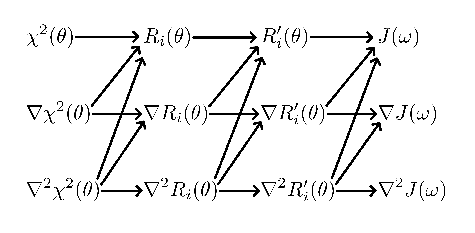
\includegraphics[width=0.8\textwidth, bb=14 14 226 110]{images/dependencies.eps.gz}}
\caption[$\chi^2$ dependencies of the values, gradients, and Hessians.]{Dependencies between the $\chi^2$, transformed relaxation, relaxation, and spectral density equations, gradients, and Hessians.}\label{fig: dependencies}
\end{figure}



% The chi-squared value, gradient, and Hessian.
%%%%%%%%%%%%%%%%%%%%%%%%%%%%%%%%%%%%%%%%%%%%%%%

\begin{latexonly}
    \section{The $\chi^2$ value, gradient, and Hessian}
\end{latexonly}
\begin{htmlonly}
    \section{The chi-squared value, gradient, and Hessian}
\end{htmlonly}

% The chi-squared value.
\begin{latexonly}
    \subsection{The $\chi^2$ value}
\end{latexonly}
\begin{htmlonly}
    \subsection{The chi-squared value}
\end{htmlonly}

The $\chi^2$ value is defined as
\begin{equation} \label{eq: maths: chi-squared}
 \chi^2(\theta) = \sum_{i=1}^n \frac{(\Ri - \Ri(\theta))^2}{\sigma_i^2},
\end{equation}

\noindent where the summation index $i$ ranges over all the relaxation data of all residues used in the analysis.



% The chi-squared gradient.
\begin{latexonly}
    \subsection{The $\chi^2$ gradient}
\end{latexonly}
\begin{htmlonly}
    \subsection{The chi-squared gradient}
\end{htmlonly}

The $\chi^2$ gradient in vector notation is
\begin{equation}
 \nabla \chi^2(\theta) = 2 \sum_{i=1}^n \frac{(\Ri - \Ri(\theta))^2}{\sigma_i^2} \nabla \Ri(\theta).
\end{equation}



% The chi-squared Hessian.
\begin{latexonly}
    \subsection{The $\chi^2$ Hessian}
\end{latexonly}
\begin{htmlonly}
    \subsection{The chi-squared Hessian}
\end{htmlonly}

The $\chi^2$ Hessian in vector notation is
\begin{equation}
 \nabla^2 \chi^2(\theta) = 2 \sum_{i=1}^n \frac{1}{\sigma_i^2} \left(\nabla \Ri(\theta) \cdot \nabla \Ri(\theta)^T - (\Ri - \Ri(\theta)) \nabla^2 \Ri(\theta) \right).
\end{equation}



% The Ri values, gradients, and Hessians.
%%%%%%%%%%%%%%%%%%%%%%%%%%%%%%%%%%%%%%%%%

\newpage
\begin{latexonly}
    \section{The $\Ri(\theta)$ values, gradients, and Hessians}
\end{latexonly}
\begin{htmlonly}
    \section{The R$_i(theta)$ values, gradients, and Hessians}
\end{htmlonly}


% The Ri values.
\begin{latexonly}
    \subsection{The $\Ri(\theta)$ values}
\end{latexonly}
\begin{htmlonly}
    \subsection{The R$_i(theta)$ values}
\end{htmlonly}

The $\Ri(\theta)$ values are given by
\begin{subequations}
\begin{align}
    \Rone(\theta) & = \Rone'(\theta), \label{eq: Ri trans: R1} \\
    \Rtwo(\theta) & = \Rtwo'(\theta), \label{eq: Ri trans: R2} \\
    \mathrm{NOE}(\theta) & = 1 + \frac{\gH}{\gX} \frac{\crossrate(\theta)}{\Rone(\theta)}. \label{eq: Ri trans: NOE}
\end{align}
\end{subequations}


% The Ri gradients.
\begin{latexonly}
    \subsection{The $\Ri(\theta)$ gradients}
\end{latexonly}
\begin{htmlonly}
    \subsection{The R$_i(theta)$ gradients}
\end{htmlonly}

The $\Ri(\theta)$ gradients in vector notation are
\begin{subequations}
\begin{align}
    \nabla \Rone(\theta) & = \nabla \Rone'(\theta), \label{eq: Ri trans: dR1} \\
    \nabla \Rtwo(\theta) & = \nabla \Rtwo'(\theta), \label{eq: Ri trans: dR2} \\
    \nabla \mathrm{NOE}(\theta) & = \frac{\gH}{\gX} \frac{1}{\Rone(\theta)^2} \Big(
        \Rone(\theta) \nabla \crossrate(\theta) - \crossrate(\theta) \nabla \Rone(\theta)
    \Big). \label{eq: Ri trans: dNOE}
\end{align}
\end{subequations}


% The Ri Hessians.
\begin{latexonly}
    \subsection{The $\Ri(\theta)$ Hessians}
\end{latexonly}
\begin{htmlonly}
    \subsection{The R$_i(theta)$ Hessians}
\end{htmlonly}

The $\Ri(\theta)$ Hessians in vector notation are
\begin{subequations}
\begin{align}
    \nabla^2 \Rone(\theta) & = \nabla^2 \Rone'(\theta), \label{eq: Ri trans: d2R1} \\
    \nabla^2 \Rtwo(\theta) & = \nabla^2 \Rtwo'(\theta), \label{eq: Ri trans: d2R2} \\
    \nabla^2 \mathrm{NOE}(\theta) & = \frac{\gH}{\gX} \frac{1}{\Rone(\theta)^3} \bigg[
        \crossrate(\theta) \Big( 2 \nabla \Rone(\theta) \cdot \nabla \Rone(\theta)^T - \Rone(\theta) \nabla^2 \Rone(\theta) \Big) \nonumber\\
        & \quad - \Rone(\theta) \Big( \nabla \crossrate(\theta) \cdot \nabla \Rone(\theta)^T - \Rone(\theta) \nabla^2 \crossrate(\theta) \Big)
    \bigg]. \label{eq: Ri trans: d2NOE}
\end{align}
\end{subequations}



% Ri' values, gradients, and Hessians.
%%%%%%%%%%%%%%%%%%%%%%%%%%%%%%%%%%%%%%

\newpage
\begin{latexonly}
    \section{$\Ri'(\theta)$ values, gradients, and Hessians}
\end{latexonly}
\begin{htmlonly}
    \section{R$_i$ $prime(theta)$ values, gradients, and Hessians}
\end{htmlonly}

The partial and second partial derivatives of the relaxation equations of the set R$'(\theta)$ are different for each parameter of the vector $\theta$.  The vector representation of the gradient $\nabla \textrm{R}_i'(\theta)$ and the matrix representation of the Hessian $\nabla^2 \textrm{R}_i'(\theta)$ can be reconstructed from the individual elements presented in the next section.


% Components.
%~~~~~~~~~~~~

\begin{latexonly}
    \subsection{Components of the $\Ri'(\theta)$ equations}
\end{latexonly}
\begin{htmlonly}
    \subsection{Components of the R$_i$ $prime(theta)$ equations}
\end{htmlonly}


To simplify the calculations of the gradients and Hessians the $\Ri'(\theta)$ equations have been broken down into a number of components.  These include the dipolar and CSA constants as well as the dipolar and CSA spectral density terms for each of the three transformed relaxation data types \{$\Rone$, $\Rtwo$, $\crossrate$\}.  The segregation of these components simplifies the maths as many partial derivatives of the components are zero.


% Dipolar comps.
\subsubsection{Dipolar constant}

The dipolar constant is defined as
\begin{equation}
    d = \frac{1}{4} \left(\frac{\mu_0}{4\pi}\right)^2 \frac{\left( \gH \gX \hbar \right)^2}{<r^6>}. \label{eq: Ri': d}
\end{equation}

\noindent This component of the relaxation equations is independent of the parameter of the spectral density function $\theta_j$, the chemical exchange parameter $\rho_{ex}$, and the CSA parameter $\Delta\sigma$.  Therefore the partial and second partial derivatives with respect to these parameters is zero.  Only the derivative with respect to the bond length $r$ is non-zero being
\begin{equation}
    d' \equiv \frac{\mathrm{d} d}{\mathrm{d} r} = - \frac{3}{2} \left(\frac{\mu_0}{4\pi}\right)^2 \frac{\left( \gH \gX \hbar \right)^2}{<r^7>}. \label{eq: Ri': d'}
\end{equation}

\noindent The second derivative with respect to the bond length is
\begin{equation}
    d'' \equiv \frac{\mathrm{d}^2 d}{\mathrm{d} r^2} = \frac{21}{2} \left(\frac{\mu_0}{4\pi}\right)^2 \frac{\left( \gH \gX \hbar \right)^2}{<r^8>}. \label{eq: Ri': d"}
\end{equation}


% CSA comps.
\subsubsection{CSA constant}

The CSA constant is defined as
\begin{equation}
    c = \frac{\left(\omega_X \cdot \Delta\sigma \right)^2}{3}. \label{eq: Ri': c}
\end{equation}

\noindent The partial derivative of this component with respect to all parameters but the CSA parameter $\Delta\sigma$ is zero.  This derivative is
\begin{equation}
    c' \equiv \frac{\mathrm{d} c}{\mathrm{d} \Delta\sigma} = \frac{2 \omega_X^2 \cdot \Delta\sigma}{3}. \label{eq: Ri': c'}
\end{equation}

\noindent The CSA constant second derivative with respect to $\Delta\sigma$ is
\begin{equation}
    c'' \equiv \frac{\mathrm{d}^2 c}{\mathrm{d} \Delta\sigma^2} = \frac{2 \omega_X^2}{3}. \label{eq: Ri': c"}
\end{equation}


% Rex comps.
\subsubsection{$R_{ex}$ constant}

The $R_{ex}$ constant is defined as
\begin{equation}
    R_{ex} = \rho_{ex} (2 \pi \omega_H)^2 . \label{eq: Ri': Rex}
\end{equation}

\noindent The partial derivative of this component with respect to all parameters but the chemical exchange parameter $\rho_{ex}$ is zero.  This derivative is
\begin{equation}
    R_{ex}' \equiv \frac{\mathrm{d} R_{ex}}{\mathrm{d} \rho_{ex}} = (2 \pi \omega_H)^2. \label{eq: Ri': Rex'}
\end{equation}

\noindent The $R_{ex}$ constant second derivative with respect to $\rho_{ex}$ is
\begin{equation}
    R_{ex}'' \equiv \frac{\mathrm{d}^2 R_{ex}}{\mathrm{d} \rho_{ex}^2} = 0. \label{eq: Ri': Rex"}
\end{equation}


% R1 dip Spectral density terms.
\subsubsection{Spectral density terms of the $\Rone$ dipolar component}

For the dipolar component of the $\Rone$ equation~\eqref{eq: R1} on page~\pageref{eq: R1} the spectral density terms are
\begin{equation}
    J_d^{\Rone} = J(\omega_H - \omega_X) + 3J(\omega_X) + 6J(\omega_H + \omega_X).  \label{eq: J terms: JR1d}
\end{equation}

\noindent The partial derivative of these terms with respect to the spectral density function parameter $\theta_j$ is
\begin{equation}
    {J_d^{\Rone}}' \equiv \frac{\partial J_d^{\Rone}}{\partial \theta_j}
        = \frac{\partial J(\omega_H - \omega_X)}{\partial \theta_j}
        + 3 \frac{\partial J(\omega_X)}{\partial \theta_j}
        + 6 \frac{\partial J(\omega_H + \omega_X)}{\partial \theta_j}.  \label{eq: J terms: JR1d'}
\end{equation}

\noindent The second partial derivative with respect to the spectral density function parameters $\theta_j$ and $\theta_k$ is
\begin{equation}
    {J_d^{\Rone}}'' \equiv \frac{\partial^2 J_d^{\Rone}}{\partial \theta_j \cdot \partial \theta_k}
        = \frac{\partial^2 J(\omega_H - \omega_X)}{\partial \theta_j \cdot \partial \theta_k}
        + 3 \frac{\partial^2 J(\omega_X)}{\partial \theta_j \cdot \partial \theta_k}
        + 6 \frac{\partial^2 J(\omega_H + \omega_X)}{\partial \theta_j \cdot \partial \theta_k}.  \label{eq: J terms: JR1d"}
\end{equation}


% R1 CSA Spectral density terms.
\subsubsection{Spectral density terms of the $\Rone$ CSA component}

For the CSA component of the $\Rone$ equation~\eqref{eq: R1} on page~\pageref{eq: R1} the spectral density terms are
\begin{equation}
    J_c^{\Rone} = J(\omega_X).  \label{eq: J terms: JR1c}
\end{equation}

\noindent The partial derivative of these terms with respect to the spectral density function parameter $\theta_j$ is
\begin{equation}
    {J_c^{\Rone}}' \equiv \frac{\partial J_c^{\Rone}}{\partial \theta_j}
        = \frac{\partial J(\omega_X)}{\partial \theta_j}.  \label{eq: J terms: JR1c'}
\end{equation}

\noindent The second partial derivative with respect to the spectral density function parameters $\theta_j$ and $\theta_k$ is
\begin{equation}
    {J_c^{\Rone}}'' \equiv \frac{\partial^2 J_c^{\Rone}}{\partial \theta_j . \partial \theta_k}
        = \frac{\partial^2 J(\omega_X)}{\partial \theta_j \cdot \partial \theta_k}.  \label{eq: J terms: JR1c"}
\end{equation}


% R2 dip Spectral density terms.
\subsubsection{Spectral density terms of the $\Rtwo$ dipolar component}

For the dipolar component of the $\Rtwo$ equation~\eqref{eq: R2} on page~\pageref{eq: R2} the spectral density terms are
\begin{equation}
    J_d^{\Rtwo} = 4J(0) + J(\omega_H - \omega_X) + 3J(\omega_X) + 6J(\omega_H) + 6J(\omega_H + \omega_X).  \label{eq: J terms: JR2d}
\end{equation}

\noindent The partial derivative of these terms with respect to the spectral density function parameter $\theta_j$ is
\begin{equation}
    {J_d^{\Rtwo}}' \equiv \frac{\partial J_d^{\Rtwo}}{\partial \theta_j}
        = 4 \frac{\partial J(0)}{\partial \theta_j}
        + \frac{\partial J(\omega_H - \omega_X)}{\partial \theta_j}
        + 3 \frac{\partial J(\omega_X)}{\partial \theta_j}
        + 6 \frac{\partial J(\omega_H)}{\partial \theta_j}
        + 6 \frac{\partial J(\omega_H + \omega_X)}{\partial \theta_j}.  \label{eq: J terms: JR2d'}
\end{equation}

\noindent The second partial derivative with respect to the spectral density function parameters $\theta_j$ and $\theta_k$ is
\begin{multline}
    {J_d^{\Rtwo}}'' \equiv \frac{\partial^2 J_d^{\Rtwo}}{\partial \theta_j \cdot \partial \theta_k}
        = 4 \frac{\partial^2 J(0)}{\partial \theta_j \cdot \partial \theta_k}
        + \frac{\partial^2 J(\omega_H - \omega_X)}{\partial \theta_j \cdot \partial \theta_k}
        + 3 \frac{\partial^2 J(\omega_X)}{\partial \theta_j \cdot \partial \theta_k} \\
        + 6 \frac{\partial^2 J(\omega_H)}{\partial \theta_j \cdot \partial \theta_k}
        + 6 \frac{\partial^2 J(\omega_H + \omega_X)}{\partial \theta_j \cdot \partial \theta_k}.  \label{eq: J terms: JR2d"}
\end{multline}


% R2 CSA Spectral density terms.
\subsubsection{Spectral density terms of the $\Rtwo$ CSA component}

For the CSA component of the $\Rtwo$ equation~\eqref{eq: R2} on page~\pageref{eq: R2} the spectral density terms are
\begin{equation}
    J_c^{\Rtwo} = 4J(0) + 3J(\omega_X).  \label{eq: J terms: JR2c}
\end{equation}

\noindent The partial derivative of these terms with respect to the spectral density function parameter $\theta_j$ is
\begin{equation}
    {J_c^{\Rtwo}}' \equiv \frac{\partial J_c^{\Rtwo}}{\partial \theta_j}
        = 4 \frac{\partial J(0)}{\partial \theta_j}
        + 3 \frac{\partial J(\omega_X)}{\partial \theta_j}.  \label{eq: J terms: JR2c'}
\end{equation}

\noindent The second partial derivative with respect to the spectral density function parameters $\theta_j$ and $\theta_k$ is
\begin{equation}
    {J_c^{\Rtwo}}'' \equiv \frac{\partial^2 J_c^{\Rtwo}}{\partial \theta_j \cdot \partial \theta_k}
        = 4 \frac{\partial^2 J(0)}{\partial \theta_j \cdot \partial \theta_k}
        + 3 \frac{\partial^2 J(\omega_X)}{\partial \theta_j \cdot \partial \theta_k}.  \label{eq: J terms: JR2c"}
\end{equation}


% Sigma_NOE dip Spectral density terms.
\begin{latexonly}
    \subsubsection{Spectral density terms of the $\crossrate$ dipolar component}
\end{latexonly}
\begin{htmlonly}
    \subsubsection{Spectral density terms of the $sigma_{NOE}$ dipolar component}
\end{htmlonly}

For the dipolar component of the $\crossrate$ equation~\eqref{eq: sigma_NOE} on page~\pageref{eq: sigma_NOE} the spectral density terms are
\begin{equation}
    J_d^{\crossrate} = 6J(\omega_H + \omega_X) - J(\omega_H - \omega_X).  \label{eq: J terms: JsigmaNOEd}
\end{equation}

\noindent The partial derivative of these terms with respect to the spectral density function parameter $\theta_j$ is
\begin{equation}
    {J_d^{\crossrate}}' \equiv \frac{\partial J_d^{\crossrate}}{\partial \theta_j}
        = 6 \frac{\partial J(\omega_H + \omega_X)}{\partial \theta_j}
          - \frac{\partial J(\omega_H - \omega_X)}{\partial \theta_j}.  \label{eq: J terms: JsigmaNOEd'}
\end{equation}

\noindent The second partial derivative with respect to the spectral density function parameters $\theta_j$ and $\theta_k$ is
\begin{equation}
    {J_d^{\crossrate}}'' \equiv \frac{\partial^2 J_d^{\crossrate}}{\partial \theta_j \cdot \partial \theta_k}
        = 6 \frac{\partial^2 J(\omega_H + \omega_X)}{\partial \theta_j \cdot \partial \theta_k}
          - \frac{\partial^2 J(\omega_H - \omega_X)}{\partial \theta_j \cdot \partial \theta_k}.  \label{eq: J terms: JsigmaNOEd"}
\end{equation}



% Ri' values.
%~~~~~~~~~~~~

\begin{latexonly}
    \subsection{$\Ri'(\theta)$ values}
\end{latexonly}
\begin{htmlonly}
    \subsection{R$_i$ $prime(theta)$ values}
\end{htmlonly}

Using the components of the relaxation equations defined above the three relaxation equations can be re-expressed as
\begin{subequations}
\begin{align}
    \Rone(\theta) & = d J_d^{\Rone} + c J_c^{\Rone},                          \label{eq: Ri': R1} \\
    \Rtwo(\theta) & = \frac{d}{2} J_d^{\Rtwo} + \frac{c}{6} J_c^{\Rtwo},      \label{eq: Ri': R2} \\
    \crossrate(\theta) & = d J_d^{\crossrate}.                          \label{eq: Ri': sigmaNOE}
\end{align}
\end{subequations}



% Ri' gradients.
%~~~~~~~~~~~~~~~

\begin{latexonly}
    \subsection{$\Ri'(\theta)$ gradients}
\end{latexonly}
\begin{htmlonly}
    \subsection{R$_i$ $prime(theta)$ gradients}
\end{htmlonly}

A different partial derivative exists for the spectral density function parameter $\theta_j$, the chemical exchange parameter $\rho_{ex}$, CSA parameter $\Delta\sigma$, and bond length parameter $r$.  In model-free analysis the spectral density parameters include both the parameters of the diffusion tensor and the parameters of the various model-free models.


% Spectral density function parameter.
\begin{latexonly}
    \subsubsection{$\theta_j$ partial derivative}
\end{latexonly}
\begin{htmlonly}
    \subsubsection{$theta_j$ partial derivative}
\end{htmlonly}

The partial derivatives of the relaxation equations with respect to the spectral density function parameter $\theta_j$ are
\begin{subequations}
\begin{align}
    \frac{\partial \Rone(\theta)}{\partial \theta_j} &= d {J_d^{\Rone}}' + c {J_c^{\Rone}}',                      \label{eq: Ri': dR1/dmf} \\
    \frac{\partial \Rtwo(\theta)}{\partial \theta_j} &= \frac{d}{2} {J_d^{\Rtwo}}' + \frac{c}{6} {J_c^{\Rtwo}}',  \label{eq: Ri': dR2/dmf} \\
    \frac{\partial \crossrate(\theta)}{\partial \theta_j} &= d {J_d^{\crossrate}}'.                         \label{eq: Ri': dsigmaNOE/dmf}
\end{align}
\end{subequations}


% Chemical exchange parameter.
\begin{latexonly}
    \subsubsection{$\rho_{ex}$ partial derivative}
\end{latexonly}
\begin{htmlonly}
    \subsubsection{$rho_{ex}$ partial derivative}
\end{htmlonly}

The partial derivatives of the relaxation equations with respect to the chemical exchange parameter $\rho_{ex}$ are
\begin{subequations}
\begin{align}
    \frac{\partial \Rone(\theta)}{\partial \rho_{ex}} &= 0,          \label{eq: Ri': dR1/dRex} \\
    \frac{\partial \Rtwo(\theta)}{\partial \rho_{ex}} &= (2 \pi \omega_H)^2,          \label{eq: Ri': dR2/dRex} \\
    \frac{\partial \crossrate(\theta)}{\partial \rho_{ex}} &= 0.   \label{eq: Ri': dsigmaNOE/dRex}
\end{align}
\end{subequations}


% CSA parameter.
\begin{latexonly}
    \subsubsection{$\Delta\sigma$ partial derivative}
\end{latexonly}
\begin{htmlonly}
    \subsubsection{$D_{sigma}$ partial derivative}
\end{htmlonly}

The partial derivatives of the relaxation equations with respect to the CSA parameter $\Delta\sigma$ are
\begin{subequations}
\begin{align}
    \frac{\partial \Rone(\theta)}{\partial \Delta\sigma} &= c' J_c^{\Rone},             \label{eq: Ri': dR1/dCSA} \\
    \frac{\partial \Rtwo(\theta)}{\partial \Delta\sigma} &= \frac{c'}{6} J_c^{\Rtwo},   \label{eq: Ri': dR2/dCSA} \\
    \frac{\partial \crossrate(\theta)}{\partial \Delta\sigma} &= 0.                 \label{eq: Ri': dsigmaNOE/dCSA}
\end{align}
\end{subequations}


% Bond length parameter.
\subsubsection{$r$ partial derivative}

The partial derivatives of the relaxation equations with respect to the bond length parameter $r$ are
\begin{subequations}
\begin{align}
    \frac{\partial \Rone(\theta)}{\partial r} &= d' J_d^{\Rone},                \label{eq: Ri': dR1/dr} \\
    \frac{\partial \Rtwo(\theta)}{\partial r} &= \frac{d'}{2} J_d^{\Rtwo},      \label{eq: Ri': dR2/dr} \\
    \frac{\partial \crossrate(\theta)}{\partial r} &= d' J_d^{\crossrate}.  \label{eq: Ri': dsigmaNOE/dr}
\end{align}
\end{subequations}



% Ri' Hessians.
%~~~~~~~~~~~~~~

\begin{latexonly}
    \subsection{$\Ri'(\theta)$ Hessians}
\end{latexonly}
\begin{htmlonly}
    \subsection{R$_i$ $prime(theta)$ Hessians}
\end{htmlonly}

Again different second partial derivatives with respect to the spectral density function parameters $\theta_j$ and $\theta_k$, the chemical exchange parameter $\rho_{ex}$, CSA parameter $\Delta\sigma$, and bond length parameter $r$.  These second partial derivatives are the components of the $\Ri'(\theta)$ Hessian matrices.


% Spectral density function parameter -- Spectral density function parameter.
\begin{latexonly}
    \subsubsection{$\theta_j$ -- $\theta_k$ partial derivative}
\end{latexonly}
\begin{htmlonly}
    \subsubsection{$theta_j$ -- $theta_k$ partial derivative}
\end{htmlonly}

The second partial derivatives of the relaxation equations with respect to the spectral density function parameters $\theta_j$ and $\theta_k$ are
\begin{subequations}
\begin{align}
    \frac{\partial^2 \Rone(\theta)}{\partial \theta_j \cdot \partial \theta_k} &= d {J_d^{\Rone}}'' + c {J_c^{\Rone}}'',                      \label{eq: Ri': d2R1/dmfj.dmfk} \\
    \frac{\partial^2 \Rtwo(\theta)}{\partial \theta_j \cdot \partial \theta_k} &= \frac{d}{2} {J_d^{\Rtwo}}'' + \frac{c}{6} {J_c^{\Rtwo}}'',  \label{eq: Ri': d2R2/dmfj.dmfk} \\
    \frac{\partial^2 \crossrate(\theta)}{\partial \theta_j \cdot \partial \theta_k} &= d {J_d^{\crossrate}}''.                          \label{eq: Ri': d2sigmaNOE/dmfj.dmfk}
\end{align}
\end{subequations}


% Spectral density function parameter -- Chemical exchange parameter.
\begin{latexonly}
    \subsubsection{$\theta_j$ -- $\rho_{ex}$ partial derivative}
\end{latexonly}
\begin{htmlonly}
    \subsubsection{$theta_j$ -- $rho_{ex}$ partial derivative}
\end{htmlonly}

The second partial derivatives of the relaxation equations with respect to the spectral density function parameter $\theta_j$ and the chemical exchange parameter $\rho_{ex}$ are
\begin{subequations}
\begin{align}
    \frac{\partial^2 \Rone(\theta)}{\partial \theta_j \cdot \partial \rho_{ex}} &= 0,        \label{eq: Ri': d2R1/dmfj.dRex} \\
    \frac{\partial^2 \Rtwo(\theta)}{\partial \theta_j \cdot \partial \rho_{ex}} &= 0,        \label{eq: Ri': d2R2/dmfj.dRex} \\
    \frac{\partial^2 \crossrate(\theta)}{\partial \theta_j \cdot \partial \rho_{ex}} &= 0. \label{eq: Ri': d2sigmaNOE/dmfj.dRex}
\end{align}
\end{subequations}


% Spectral density function parameter -- CSA parameter.
\begin{latexonly}
    \subsubsection{$\theta_j$ -- $\Delta\sigma$ partial derivative}
\end{latexonly}
\begin{htmlonly}
    \subsubsection{$theta_j$ -- $D_{sigma}$ partial derivative}
\end{htmlonly}

The second partial derivatives of the relaxation equations with respect to the spectral density function parameter $\theta_j$ and the CSA parameter $\Delta\sigma$ are
\begin{subequations}
\begin{align}
    \frac{\partial^2 \Rone(\theta)}{\partial \theta_j \cdot \partial \Delta\sigma} &= c' {J_c^{\Rone}}',            \label{eq: Ri': d2R1/dmfj.dCSA} \\
    \frac{\partial^2 \Rtwo(\theta)}{\partial \theta_j \cdot \partial \Delta\sigma} &= \frac{c'}{6} {J_c^{\Rtwo}}',  \label{eq: Ri': d2R2/dmfj.dCSA} \\
    \frac{\partial^2 \crossrate(\theta)}{\partial \theta_j \cdot \partial \Delta\sigma} &= 0.                   \label{eq: Ri': d2sigmaNOE/dmfj.dCSA}
\end{align}
\end{subequations}


% Spectral density function parameter -- Bond length parameter.
\begin{latexonly}
    \subsubsection{$\theta_j$ -- $r$ partial derivative}
\end{latexonly}
\begin{htmlonly}
    \subsubsection{$theta_j$ -- $r$ partial derivative}
\end{htmlonly}

The second partial derivatives of the relaxation equations with respect to the spectral density function parameter $\theta_j$ and the bond length parameter $r$ are
\begin{subequations}
\begin{align}
    \frac{\partial^2 \Rone(\theta)}{\partial \theta_j \cdot \partial r} &= d' {J_d^{\Rone}}',               \label{eq: Ri': d2R1/dmfj.dr} \\
    \frac{\partial^2 \Rtwo(\theta)}{\partial \theta_j \cdot \partial r} &= \frac{d'}{2} {J_d^{\Rtwo}}',     \label{eq: Ri': d2R2/dmfj.dr} \\
    \frac{\partial^2 \crossrate(\theta)}{\partial \theta_j \cdot \partial r} &= d' {J_d^{\crossrate}}'. \label{eq: Ri': d2sigmaNOE/dmfj.dr}
\end{align}
\end{subequations}


% Chemical exchange parameter -- Chemical exchange parameter.
\begin{latexonly}
    \subsubsection{$\rho_{ex}$ -- $\rho_{ex}$ partial derivative}
\end{latexonly}
\begin{htmlonly}
    \subsubsection{$rho_{ex}$ -- $rho_{ex}$ partial derivative}
\end{htmlonly}

The second partial derivatives of the relaxation equations with respect to the chemical exchange parameter $\rho_{ex}$ twice are
\begin{subequations}
\begin{align}
    \frac{\partial^2 \Rone(\theta)}{{\partial \rho_{ex}}^2} &= 0,        \label{eq: Ri': d2R1/dRex2} \\
    \frac{\partial^2 \Rtwo(\theta)}{{\partial \rho_{ex}}^2} &= 0,        \label{eq: Ri': d2R2/dRex2} \\
    \frac{\partial^2 \crossrate(\theta)}{{\partial \rho_{ex}}^2} &= 0. \label{eq: Ri': d2sigmaNOE/dRex2}
\end{align}
\end{subequations}


% Chemical exchange parameter -- CSA parameter.
\begin{latexonly}
    \subsubsection{$\rho_{ex}$ -- $\Delta\sigma$ partial derivative}
\end{latexonly}
\begin{htmlonly}
    \subsubsection{$rho_{ex}$ -- $D_{sigma}$ partial derivative}
\end{htmlonly}

The second partial derivatives of the relaxation equations with respect to the chemical exchange parameter $\rho_{ex}$ and the CSA parameter $\Delta\sigma$ are
\begin{subequations}
\begin{align}
    \frac{\partial^2 \Rone(\theta)}{\partial \rho_{ex} \cdot \partial \Delta\sigma} &= 0,        \label{eq: Ri': d2R1/dRex.dCSA} \\
    \frac{\partial^2 \Rtwo(\theta)}{\partial \rho_{ex} \cdot \partial \Delta\sigma} &= 0,        \label{eq: Ri': d2R2/dRex.dCSA} \\
    \frac{\partial^2 \crossrate(\theta)}{\partial \rho_{ex} \cdot \partial \Delta\sigma} &= 0. \label{eq: Ri': d2sigmaNOE/dRex.dCSA}
\end{align}
\end{subequations}


% Chemical exchange parameter -- Bond length parameter.
\begin{latexonly}
    \subsubsection{$\rho_{ex}$ -- $r$ partial derivative}
\end{latexonly}
\begin{htmlonly}
    \subsubsection{$rho_{ex}$ -- $r$ partial derivative}
\end{htmlonly}

The second partial derivatives of the relaxation equations with respect to the chemical exchange parameter $\rho_{ex}$ and the bond length parameter $r$ are
\begin{subequations}
\begin{align}
    \frac{\partial^2 \Rone(\theta)}{\partial \rho_{ex} \cdot \partial r} &= 0,           \label{eq: Ri': d2R1/dRex.dr} \\
    \frac{\partial^2 \Rtwo(\theta)}{\partial \rho_{ex} \cdot \partial r} &= 0,           \label{eq: Ri': d2R2/dRex.dr} \\
    \frac{\partial^2 \crossrate(\theta)}{\partial \rho_{ex} \cdot \partial r} &= 0.    \label{eq: Ri': d2sigmaNOE/dRex.dr}
\end{align}
\end{subequations}


% CSA parameter -- CSA parameter.
\begin{latexonly}
    \subsubsection{$\Delta\sigma$ -- $\Delta\sigma$ partial derivative}
\end{latexonly}
\begin{htmlonly}
    \subsubsection{$D_{sigma}$ -- $D_{sigma}$ partial derivative}
\end{htmlonly}

The second partial derivatives of the relaxation equations with respect to the CSA parameter $\Delta\sigma$ twice are
\begin{subequations}
\begin{align}
    \frac{\partial^2 \Rone(\theta)}{{\partial \Delta\sigma}^2} &= c'' J_c^{\Rone},              \label{eq: Ri': d2R1/dCSA2} \\
    \frac{\partial^2 \Rtwo(\theta)}{{\partial \Delta\sigma}^2} &= \frac{c''}{6} J_c^{\Rtwo},    \label{eq: Ri': d2R2/dCSA2} \\
    \frac{\partial^2 \crossrate(\theta)}{{\partial \Delta\sigma}^2} &= 0.                   \label{eq: Ri': d2sigmaNOE/dCSA2}
\end{align}
\end{subequations}


% CSA parameter -- Bond length parameter.
\begin{latexonly}
    \subsubsection{$\Delta\sigma$ -- $r$ partial derivative}
\end{latexonly}
\begin{htmlonly}
    \subsubsection{$D_{sigma}$ -- $r$ partial derivative}
\end{htmlonly}

The second partial derivatives of the relaxation equations with respect to the CSA parameter $\Delta\sigma$ and the bond length parameter $r$ are
\begin{subequations}
\begin{align}
    \frac{\partial^2 \Rone(\theta)}{\partial \Delta\sigma \cdot \partial r} &= 0,         \label{eq: Ri': d2R1/dCSA.dr} \\
    \frac{\partial^2 \Rtwo(\theta)}{\partial \Delta\sigma \cdot \partial r} &= 0,         \label{eq: Ri': d2R2/dCSA.dr} \\
    \frac{\partial^2 \crossrate(\theta)}{\partial \Delta\sigma \cdot \partial r} &= 0.  \label{eq: Ri': d2sigmaNOE/dCSA.dr}
\end{align}
\end{subequations}


% Bond length parameter -- Bond length parameter.
\subsubsection{$r$ -- $r$ partial derivative}

The second partial derivatives of the relaxation equations with respect to the bond length parameter $r$ twice are
\begin{subequations}
\begin{align}
    \frac{\partial^2 \Rone(\theta)}{{\partial r}^2} &= d'' J_d^{\Rone},                 \label{eq: Ri': d2R1/dr2} \\
    \frac{\partial^2 \Rtwo(\theta)}{{\partial r}^2} &= \frac{d''}{2} J_d^{\Rtwo},       \label{eq: Ri': d2R2/dr2} \\
    \frac{\partial^2 \crossrate(\theta)}{{\partial r}^2} &= d'' J_d^{\crossrate}.   \label{eq: Ri': d2sigmaNOE/dr2}
\end{align}
\end{subequations}




% Model-free analysis.
%%%%%%%%%%%%%%%%%%%%%%

\newpage
\section{Model-free analysis}



% The model-free equations.
%~~~~~~~~~~~~~~~~~~~~~~~~~~

\subsection{The model-free equations}

In the original model-free analysis of \cite{LipariSzabo82a} the correlation function $C(\tau)$ of the XH bond vector is approximated by decoupling the internal fluctuations of the bond vector $C_\mathrm{I}(\tau)$ from the correlation function of the overall Brownian rotational diffusion $C_\mathrm{O}(\tau)$ by the equation
\begin{equation}
    C(\tau) = C_\mathrm{O}(\tau) \cdot C_\mathrm{I}(\tau).
\end{equation}

\noindent The overall correlation functions of the diffusion of a sphere, spheroid, and ellipsoid are presented respectively in section~\ref{ellipsoid equation} on page~\pageref{ellipsoid equation}, section~\ref{spheroid equation} on page~\pageref{spheroid equation}, and section~\ref{sphere equation} on page~\pageref{sphere equation}.  These three different equations can be combined into one generic correlation function which is independent of the type of diffusion.  This generic correlation function is
\begin{equation}
    C_\mathrm{O}(\tau) = \frac{1}{5} \sum_{i=-k}^k c_i \cdot e^{-\tau/\tau_i},
\end{equation}

\noindent where $c_i$ are the weights and $\tau_i$ are correlation times of the exponential terms.  In the original model-free analysis of \citet{LipariSzabo82a,LipariSzabo82b} the internal motions are modelled by the correlation function
\begin{equation}
    C_\mathrm{I}(\tau) = S^2 + (1 - S^2) e^{-\tau / \tau_e},
\end{equation}

\noindent where $S^2$ is the generalised Lipari and Szabo order parameter which is related to the amplitude of the motion and $\tau_e$ is the effective correlation time which is an indicator of the timescale of the motion, albeit being dependent on the value of the order parameter.  The order parameter ranges from one for complete rigidity to zero for unrestricted motions.  Model-free theory was extended by \citet{Clore90a} to include motions on two timescales by the correlation function
\begin{equation}
    C_\mathrm{I}(\tau) = S^2 + (1 - S^2_f) e^{-\tau / \tau_f} + (S^2_f - S^2) e^{-\tau / \tau_s},
\end{equation}

\noindent where the faster of the motions is defined by the order parameter $S^2_f$ and the correlation time $\tau_f$, the slower by the parameters $S^2_s$ and $\tau_s$, and the two order parameter are related by the equation $S^2 = S^2_f \cdot S^2_s$.

The relaxation equations of \citet{Abragam61} are composed of a sum of power spectral density functions $J(\omega)$ at five frequencies.  The spectral density function is related to the correlation function as the two are a Fourier pair.  Applying the Fourier transform to the correlation function composed of the generic diffusion equation and the original model-free correlation function results in the equation
\begin{equation} \label{eq: maths: J(w) model-free generic}
    J(\omega) = \frac{2}{5} \sum_{i=-k}^k c_i \cdot \tau_i \Bigg(
        \frac{S^2}{1 + (\omega \tau_i)^2}
        + \frac{(1 - S^2)(\tau_e + \tau_i)\tau_e}{(\tau_e + \tau_i)^2 + (\omega \tau_e \tau_i)^2}
    \Bigg).
\end{equation}

The Fourier transform using the extended model-free correlation function is
\begin{equation} \label{eq: maths: J(w) model-free ext generic}
    J(\omega) = \frac{2}{5} \sum_{i=-k}^k c_i \cdot \tau_i \Bigg(
        \frac{S^2}{1 + (\omega \tau_i)^2}
        + \frac{(1 - S^2_f)(\tau_f + \tau_i)\tau_f}{(\tau_f + \tau_i)^2 + (\omega \tau_f \tau_i)^2}
        + \frac{(S^2_f - S^2)(\tau_s + \tau_i)\tau_s}{(\tau_s + \tau_i)^2 + (\omega \tau_s \tau_i)^2}
    \Bigg).
\end{equation}



% The original model-free gradient.
%~~~~~~~~~~~~~~~~~~~~~~~~~~~~~~~~~~

\subsection{The original model-free gradient}

The model-free gradient of the original spectral density function~\eqref{eq: maths: J(w) model-free generic} is the vector of partial derivatives of the function with respect to the geometric parameter $\Diffgeoset_i$, the orientational parameter $\Difforiset_i$, the order parameter $S^2$, and the internal correlation time $\tau_e$.  The positions in the vector correspond to the model parameters which are being optimised.



% Gj partial derivative.
\begin{latexonly}
    \subsubsection{$\Diffgeoset_j$ partial derivative}
\end{latexonly}
\begin{htmlonly}
    \subsubsection{$S_j$ partial derivative}
\end{htmlonly}

The partial derivative of~\eqref{eq: maths: J(w) model-free generic} with respect to the geometric parameter $\Diffgeoset_j$ is
\begin{multline}
    \frac{\partial J(\omega)}{\partial \Diffgeoset_j} = \frac{2}{5} \sum_{i=-k}^k \Bigg(
        c_i \frac{\partial \tau_i}{\partial \Diffgeoset_j} \Bigg(
            S^2 \frac{1 - (\omega \tau_i)^2}{\left(1 + (\omega \tau_i)^2 \right)^2}
            + (1 - S^2) \tau_e^2 \frac{(\tau_e + \tau_i)^2 - (\omega \tau_e \tau_i)^2}{\left((\tau_e + \tau_i)^2 + (\omega \tau_e \tau_i)^2 \right)^2}
        \Bigg) \\
        +  \frac{\partial c_i}{\partial \Diffgeoset_j} \tau_i \Bigg(
            \frac{S^2}{1 + (\omega \tau_i)^2}
            + \frac{(1 - S^2)(\tau_e + \tau_i)\tau_e}{(\tau_e + \tau_i)^2 + (\omega \tau_e \tau_i)^2}
        \Bigg)
    \Bigg).
\end{multline}



% Oj partial derivative.
\begin{latexonly}
    \subsubsection{$\Difforiset_j$ partial derivative}
\end{latexonly}
\begin{htmlonly}
    \subsubsection{$O_j$ partial derivative}
\end{htmlonly}

The partial derivative of~\eqref{eq: maths: J(w) model-free generic} with respect to the orientational parameter $\Difforiset_j$ is
\begin{equation}
    \frac{\partial J(\omega)}{\partial \Difforiset_j} = \frac{2}{5} \sum_{i=-k}^k \frac{\partial c_i}{\partial \Difforiset_j} \tau_i \Bigg(
        \frac{S^2}{1 + (\omega \tau_i)^2}
        + \frac{(1 - S^2)(\tau_e + \tau_i)\tau_e}{(\tau_e + \tau_i)^2 + (\omega \tau_e \tau_i)^2}
    \Bigg).
\end{equation}



% S2 partial derivative.
\subsubsection{$S^2$ partial derivative}

The partial derivative of~\eqref{eq: maths: J(w) model-free generic} with respect to the order parameter $S^2$ is
\begin{equation}
    \frac{\partial J(\omega)}{\partial S^2} = \frac{2}{5} \sum_{i=-k}^k c_i \tau_i \Bigg(
        \frac{1}{1 + (\omega \tau_i)^2}
        - \frac{(\tau_e + \tau_i)\tau_e}{(\tau_e + \tau_i)^2 + (\omega \tau_e \tau_i)^2}
    \Bigg).
\end{equation}



% te partial derivative.
\begin{latexonly}
    \subsubsection{$\tau_e$ partial derivative}
\end{latexonly}
\begin{htmlonly}
    \subsubsection{$tau_e$ partial derivative}
\end{htmlonly}

The partial derivative of~\eqref{eq: maths: J(w) model-free generic} with respect to the correlation time $\tau_e$ is
\begin{equation}
    \frac{\partial J(\omega)}{\partial \tau_e} = \frac{2}{5} (1 - S^2) \sum_{i=-k}^k c_i \tau_i^2
        \frac{(\tau_e + \tau_i)^2 - (\omega \tau_e \tau_i)^2}{\left((\tau_e + \tau_i)^2 + (\omega \tau_e \tau_i)^2 \right)^2}.
\end{equation}



% The original model-free Hessian.
%~~~~~~~~~~~~~~~~~~~~~~~~~~~~~~~~~

\newpage
\subsection{The original model-free Hessian}

The model-free Hessian of the original spectral density function~\eqref{eq: maths: J(w) model-free generic} is the matrix of second partial derivatives.  The matrix coordinates correspond to the model parameters which are being optimised.



% Gj-Gk partial derivative.
\begin{latexonly}
    \subsubsection{$\Diffgeoset_j$ -- $\Diffgeoset_k$ partial derivative}
\end{latexonly}
\begin{htmlonly}
    \subsubsection{$G_j$ -- $G_k$ partial derivative}
\end{htmlonly}

The second partial derivative of~\eqref{eq: maths: J(w) model-free generic} with respect to the geometric parameters $\Diffgeoset_j$ and $\Diffgeoset_k$ is
\begin{multline}
    \frac{\partial^2 J(\omega)}{\partial \Diffgeoset_j \cdot \partial \Diffgeoset_k} = \frac{2}{5} \sum_{i=-k}^k \Bigg(
        -2 c_i \frac{\partial \tau_i}{\partial \Diffgeoset_j} \cdot \frac{\partial \tau_i}{\partial \Diffgeoset_k} \Bigg(
            S^2 \omega^2 \tau_i \frac{3 - (\omega \tau_i)^2}{\left(1 + (\omega \tau_i)^2 \right)^3}  \\
            + (1 - S^2) \tau_e^2 \frac{(\tau_e + \tau_i)^3  +  3 \omega^2 \tau_e^3 \tau_i (\tau_e + \tau_i)  -  (\omega \tau_e)^4 \tau_i^3}
                {\left((\tau_e + \tau_i)^2 + (\omega \tau_e \tau_i)^2 \right)^3}
        \Bigg) \\
        + \Bigg(
            \frac{\partial \tau_i}{\partial \Diffgeoset_j} \cdot \frac{\partial c_i}{\partial \Diffgeoset_k}
            + \frac{\partial \tau_i}{\partial \Diffgeoset_k} \cdot \frac{\partial c_i}{\partial \Diffgeoset_j}
            + c_i \frac{\partial^2 \tau_i}{\partial \Diffgeoset_j \cdot \partial \Diffgeoset_k}
        \Bigg)
        \Bigg(
            S^2 \frac{1 - (\omega \tau_i)^2}{\left(1 + (\omega \tau_i)^2 \right)^2} \\
            + (1 - S^2) \tau_e^2 \frac{(\tau_e + \tau_i)^2 - (\omega \tau_e \tau_i)^2}{\left((\tau_e + \tau_i)^2 + (\omega \tau_e \tau_i)^2 \right)^2}
        \Bigg) \\
        + \Bigg(
            \frac{\partial^2 c_i}{\partial \Diffgeoset_j \cdot \partial \Diffgeoset_k} \tau_i \Bigg(
                \frac{S^2}{1 + (\omega \tau_i)^2}
                + \frac{(1 - S^2)(\tau_e + \tau_i)\tau_e}{(\tau_e + \tau_i)^2 + (\omega \tau_e \tau_i)^2}
            \Bigg)
        \Bigg)
    \Bigg).
\end{multline}
                


% Gj-Ok partial derivative.
\begin{latexonly}
    \subsubsection{$\Diffgeoset_j$ -- $\Difforiset_k$ partial derivative}
\end{latexonly}
\begin{htmlonly}
    \subsubsection{$G_j$ -- $O_k$ partial derivative}
\end{htmlonly}

The second partial derivative of~\eqref{eq: maths: J(w) model-free generic} with respect to the geometric parameter $\Diffgeoset_j$ and the orientational parameter $\Difforiset_k$ is
\begin{multline}
    \frac{\partial^2 J(\omega)}{\partial \Diffgeoset_j \cdot \partial \Difforiset_k} = \frac{2}{5} \sum_{i=-k}^k \Bigg(
        \frac{\partial \tau_i}{\partial \Diffgeoset_j} \frac{\partial c_i}{\partial \Difforiset_k} \Bigg(
            S^2 \frac{1 - (\omega \tau_i)^2}{\left(1 + (\omega \tau_i)^2 \right)^2}
            + (1 - S^2) \tau_e^2 \frac{(\tau_e + \tau_i)^2 - (\omega \tau_e \tau_i)^2}{\left((\tau_e + \tau_i)^2 + (\omega \tau_e \tau_i)^2 \right)^2}
        \Bigg) \\
        +  \frac{\partial^2 c_i}{\partial \Diffgeoset_j \cdot \partial \Difforiset_k} \tau_i \Bigg(
            \frac{S^2}{1 + (\omega \tau_i)^2}
            + \frac{(1 - S^2)(\tau_e + \tau_i)\tau_e}{(\tau_e + \tau_i)^2 + (\omega \tau_e \tau_i)^2}
        \Bigg)
    \Bigg).
\end{multline}



% Gj-S2 partial derivative.
\begin{latexonly}
    \subsubsection{$\Diffgeoset_j$ -- $S^2$ partial derivative}
\end{latexonly}
\begin{htmlonly}
    \subsubsection{$G_j$ -- $S^2$ partial derivative}
\end{htmlonly}

The second partial derivative of~\eqref{eq: maths: J(w) model-free generic} with respect to the geometric parameter $\Diffgeoset_j$ and the order parameter $S^2$ is
\begin{multline}
    \frac{\partial^2 J(\omega)}{\partial \Diffgeoset_j \cdot \partial S^2} = \frac{2}{5} \sum_{i=-k}^k \Bigg(
        c_i \frac{\partial \tau_i}{\partial \Diffgeoset_j} \Bigg(
            \frac{1 - (\omega \tau_i)^2}{\left(1 + (\omega \tau_i)^2 \right)^2}
            - \tau_e^2 \frac{(\tau_e + \tau_i)^2 - (\omega \tau_e \tau_i)^2}{\left((\tau_e + \tau_i)^2 + (\omega \tau_e \tau_i)^2 \right)^2}
        \Bigg) \\
        +  \frac{\partial c_i}{\partial \Diffgeoset_j} \tau_i \Bigg(
            \frac{1}{1 + (\omega \tau_i)^2}
            - \frac{(\tau_e + \tau_i)\tau_e}{(\tau_e + \tau_i)^2 + (\omega \tau_e \tau_i)^2}
        \Bigg)
    \Bigg).
\end{multline}



% Gj-te partial derivative.
\begin{latexonly}
    \subsubsection{$\Diffgeoset_j$ -- $\tau_e$ partial derivative}
\end{latexonly}
\begin{htmlonly}
    \subsubsection{$G_j$ -- $tau_e$ partial derivative}
\end{htmlonly}

The second partial derivative of~\eqref{eq: maths: J(w) model-free generic} with respect to the geometric parameter $\Diffgeoset_j$ and the correlation time $\tau_e$ is
\begin{multline}
    \frac{\partial^2 J(\omega)}{\partial \Diffgeoset_j \cdot \partial \tau_e} = \frac{2}{5} (1 - S^2) \sum_{i=-k}^k \Bigg(
        2 c_i \frac{\partial \tau_i}{\partial \Diffgeoset_j} \tau_e \tau_i (\tau_e + \tau_i)
            \frac{(\tau_e + \tau_i)^2 - 3(\omega \tau_e \tau_i)^2}{\left((\tau_e + \tau_i)^2 + (\omega \tau_e \tau_i)^2 \right)^3}  \\
        + \frac{\partial c_i}{\partial \Diffgeoset_j} \tau_i^2 \frac{(\tau_e + \tau_i)^2 - (\omega \tau_e \tau_i)^2}{\left((\tau_e + \tau_i)^2 + (\omega \tau_e \tau_i)^2 \right)^2}
    \Bigg).
\end{multline}


% Oj-Ok partial derivative.
\begin{latexonly}
    \subsubsection{$\Difforiset_j$ -- $\Difforiset_k$ partial derivative}
\end{latexonly}
\begin{htmlonly}
    \subsubsection{$O_j$ -- $O_k$ partial derivative}
\end{htmlonly}

The second partial derivative of~\eqref{eq: maths: J(w) model-free generic} with respect to the orientational parameters $\Difforiset_j$ and $\Difforiset_k$ is
\begin{equation}
    \frac{\partial^2 J(\omega)}{\partial \Difforiset_j \cdot \partial \Difforiset_k} = \frac{2}{5} \sum_{i=-k}^k
        \frac{\partial^2 c_i}{\partial \Difforiset_j \cdot \partial \Difforiset_k} \tau_i \Bigg(
            \frac{S^2}{1 + (\omega \tau_i)^2}
            + \frac{(1 - S^2)(\tau_e + \tau_i)\tau_e}{(\tau_e + \tau_i)^2 + (\omega \tau_e \tau_i)^2}
        \Bigg).
\end{equation}



% Oj-S2 partial derivative.
\begin{latexonly}
    \subsubsection{$\Difforiset_j$ -- $S^2$ partial derivative}
\end{latexonly}
\begin{htmlonly}
    \subsubsection{$O_j$ -- $S^2$ partial derivative}
\end{htmlonly}

The second partial derivative of~\eqref{eq: maths: J(w) model-free generic} with respect to the orientational parameter $\Difforiset_j$ and the order parameter $S^2$ is
\begin{equation}
    \frac{\partial^2 J(\omega)}{\partial \Difforiset_j \cdot \partial S^2} = \frac{2}{5} \sum_{i=-k}^k \frac{\partial c_i}{\partial \Difforiset_j} \tau_i \Bigg(
        \frac{1}{1 + (\omega \tau_i)^2}
        - \frac{(\tau_e + \tau_i)\tau_e}{(\tau_e + \tau_i)^2 + (\omega \tau_e \tau_i)^2}
    \Bigg).
\end{equation}



% Oj-te partial derivative.
\begin{latexonly}
    \subsubsection{$\Difforiset_j$ -- $\tau_e$ partial derivative}
\end{latexonly}
\begin{htmlonly}
    \subsubsection{$O_j$ -- $tau_e$ partial derivative}
\end{htmlonly}

The second partial derivative of~\eqref{eq: maths: J(w) model-free generic} with respect to the orientational parameter $\Difforiset_j$ and the correlation time $\tau_e$ is
\begin{equation}
    \frac{\partial^2 J(\omega)}{\partial \Difforiset_j \cdot \partial \tau_e} = \frac{2}{5} (1 - S^2) \sum_{i=-k}^k
        \frac{\partial c_i}{\partial \Difforiset_j} \tau_i^2
        \frac{(\tau_e + \tau_i)^2 - (\omega \tau_e \tau_i)^2}{\left((\tau_e + \tau_i)^2 + (\omega \tau_e \tau_i)^2 \right)^2}.
\end{equation}



% S2-S2 partial derivative.
\subsubsection{$S^2$ -- $S^2$ partial derivative}

The second partial derivative of~\eqref{eq: maths: J(w) model-free generic} with respect to the order parameter $S^2$ twice is
\begin{equation}
    \frac{\partial^2 J(\omega)}{(\partial S^2)^2} = 0.
\end{equation}



% S2-te partial derivative.
\begin{latexonly}
    \subsubsection{$S^2$ -- $\tau_e$ partial derivative}
\end{latexonly}
\begin{htmlonly}
    \subsubsection{$S^2$ -- $tau_e$ partial derivative}
\end{htmlonly}

The second partial derivative of~\eqref{eq: maths: J(w) model-free generic} with respect to the order parameter $S^2$ and correlation time $\tau_e$ is
\begin{equation}
    \frac{\partial^2 J(\omega)}{\partial S^2 \cdot \partial \tau_e} = -\frac{2}{5} \sum_{i=-k}^k c_i \tau_i^2
        \frac{(\tau_e + \tau_i)^2 - (\omega \tau_e \tau_i)^2}{\left((\tau_e + \tau_i)^2 + (\omega \tau_e \tau_i)^2 \right)^2}.
\end{equation}



% te-te partial derivative.
\begin{latexonly}
    \subsubsection{$\tau_e$ -- $\tau_e$ partial derivative}
\end{latexonly}
\begin{htmlonly}
    \subsubsection{$tau_e$ -- $tau_e$ partial derivative}
\end{htmlonly}

The second partial derivative of~\eqref{eq: maths: J(w) model-free generic} with respect to the correlation time $\tau_e$ twice is
\begin{equation}
    \frac{\partial^2 J(\omega)}{{\partial \tau_e}^2} = -\frac{4}{5} (1 - S^2) \sum_{i=-k}^k c_i \tau_i^2
        \frac{(\tau_e + \tau_i)^3  +  3 \omega^2 \tau_i^3 \tau_e (\tau_e + \tau_i)  -  (\omega \tau_i)^4 \tau_e^3}
            {\left((\tau_e + \tau_i)^2 + (\omega \tau_e \tau_i)^2 \right)^3}
\end{equation}




% The extended model-free gradient.
%~~~~~~~~~~~~~~~~~~~~~~~~~~~~~~~~~~

\newpage
\subsection{The extended model-free gradient}

The model-free gradient of the extended spectral density function~\eqref{eq: maths: J(w) model-free ext generic} is the vector of partial derivatives of the function with respect to the geometric parameter $\Diffgeoset_i$, the orientational parameter $\Difforiset_i$, the order parameters $S^2$ and $S^2_f$, and the internal correlation times $\tau_f$ and $\tau_s$.  The positions in the vector correspond to the model parameters which are being optimised.



% Gj partial derivative.
\begin{latexonly}
    \subsubsection{$\Diffgeoset_j$ partial derivative}
\end{latexonly}
\begin{htmlonly}
    \subsubsection{$G_j$ partial derivative}
\end{htmlonly}

The partial derivative of~\eqref{eq: maths: J(w) model-free ext generic} with respect to the geometric parameter $\Diffgeoset_j$ is
\begin{multline}
    \frac{\partial J(\omega)}{\partial \Diffgeoset_j} = \frac{2}{5} \sum_{i=-k}^k \Bigg(
        c_i \frac{\partial \tau_i}{\partial \Diffgeoset_j} \Bigg(
            S^2 \frac{1 - (\omega \tau_i)^2}{\left(1 + (\omega \tau_i)^2 \right)^2} \\
            + (1 - S^2_f) \tau_f^2 \frac{(\tau_f + \tau_i)^2 - (\omega \tau_f \tau_i)^2}{\left((\tau_f + \tau_i)^2 + (\omega \tau_f \tau_i)^2 \right)^2} \\
            + (S^2_f - S^2) \tau_s^2 \frac{(\tau_s + \tau_i)^2 - (\omega \tau_s \tau_i)^2}{\left((\tau_s + \tau_i)^2 + (\omega \tau_s \tau_i)^2 \right)^2}
        \Bigg) \\
        +  \frac{\partial c_i}{\partial \Diffgeoset_j} \tau_i \Bigg(
            \frac{S^2}{1 + (\omega \tau_i)^2}
            + \frac{(1 - S^2_f)(\tau_f + \tau_i)\tau_f}{(\tau_f + \tau_i)^2 + (\omega \tau_f \tau_i)^2}
            + \frac{(S^2_f - S^2)(\tau_s + \tau_i)\tau_s}{(\tau_s + \tau_i)^2 + (\omega \tau_s \tau_i)^2}
        \Bigg)
    \Bigg).
\end{multline}



% Oj partial derivative.
\begin{latexonly}
    \subsubsection{$\Difforiset_j$ partial derivative}
\end{latexonly}
\begin{htmlonly}
    \subsubsection{$O_j$ partial derivative}
\end{htmlonly}

The partial derivative of~\eqref{eq: maths: J(w) model-free ext generic} with respect to the orientational parameter $\Difforiset_j$ is
\begin{equation}
    \frac{\partial J(\omega)}{\partial \Difforiset_j} = \frac{2}{5} \sum_{i=-k}^k \frac{\partial c_i}{\partial \Difforiset_j} \tau_i \Bigg(
        \frac{S^2}{1 + (\omega \tau_i)^2}
        + \frac{(1 - S^2_f)(\tau_f + \tau_i)\tau_f}{(\tau_f + \tau_i)^2 + (\omega \tau_f \tau_i)^2}
        + \frac{(S^2_f - S^2)(\tau_s + \tau_i)\tau_s}{(\tau_s + \tau_i)^2 + (\omega \tau_s \tau_i)^2}
    \Bigg).
\end{equation}



% S2 partial derivative.
\subsubsection{$S^2$ partial derivative}

The partial derivative of~\eqref{eq: maths: J(w) model-free ext generic} with respect to the order parameter $S^2$ is
\begin{equation}
    \frac{\partial J(\omega)}{\partial S^2} = \frac{2}{5} \sum_{i=-k}^k c_i \tau_i \Bigg(
        \frac{1}{1 + (\omega \tau_i)^2}
        - \frac{(\tau_s + \tau_i)\tau_s}{(\tau_s + \tau_i)^2 + (\omega \tau_s \tau_i)^2}
    \Bigg).
\end{equation}



% S2f partial derivative.
\subsubsection{$S^2_f$ partial derivative}

The partial derivative of~\eqref{eq: maths: J(w) model-free ext generic} with respect to the order parameter $S^2_f$ is
\begin{equation}
    \frac{\partial J(\omega)}{\partial S^2_f} = -\frac{2}{5} \sum_{i=-k}^k c_i \tau_i \Bigg(
        \frac{(\tau_f + \tau_i)\tau_f}{(\tau_f + \tau_i)^2 + (\omega \tau_f \tau_i)^2}
        - \frac{(\tau_s + \tau_i)\tau_s}{(\tau_s + \tau_i)^2 + (\omega \tau_s \tau_i)^2}
    \Bigg).
\end{equation}



% tf partial derivative.
\begin{latexonly}
    \subsubsection{$\tau_f$ partial derivative}
\end{latexonly}
\begin{htmlonly}
    \subsubsection{$tau_f$ partial derivative}
\end{htmlonly}

The partial derivative of~\eqref{eq: maths: J(w) model-free ext generic} with respect to the correlation time $\tau_f$ is
\begin{equation}
    \frac{\partial J(\omega)}{\partial \tau_f} = \frac{2}{5} (1 - S^2_f) \sum_{i=-k}^k c_i \tau_i^2
        \frac{(\tau_f + \tau_i)^2 - (\omega \tau_f \tau_i)^2}{\left((\tau_f + \tau_i)^2 + (\omega \tau_f \tau_i)^2 \right)^2}.
\end{equation}



% ts partial derivative.
\begin{latexonly}
    \subsubsection{$\tau_s$ partial derivative}
\end{latexonly}
\begin{htmlonly}
    \subsubsection{$tau_s$ partial derivative}
\end{htmlonly}

The partial derivative of~\eqref{eq: maths: J(w) model-free ext generic} with respect to the correlation time $\tau_s$ is
\begin{equation}
    \frac{\partial J(\omega)}{\partial \tau_s} = \frac{2}{5} (S^2_f - S^2) \sum_{i=-k}^k c_i \tau_i^2
        \frac{(\tau_s + \tau_i)^2 - (\omega \tau_s \tau_i)^2}{\left((\tau_s + \tau_i)^2 + (\omega \tau_s \tau_i)^2 \right)^2}.
\end{equation}




% The extended model-free Hessian.
%~~~~~~~~~~~~~~~~~~~~~~~~~~~~~~~~~

\newpage
\subsection{The extended model-free Hessian}

The model-free Hessian of the extended spectral density function~\eqref{eq: maths: J(w) model-free ext generic} is the matrix of second partial derivatives.  The matrix coordinates correspond to the model parameters which are being optimised.



% Gj-Gk partial derivative.
\begin{latexonly}
    \subsubsection{$\Diffgeoset_j$ -- $\Diffgeoset_k$ partial derivative}
\end{latexonly}
\begin{htmlonly}
    \subsubsection{$G_j$ -- $G_k$ partial derivative}
\end{htmlonly}

The second partial derivative of~\eqref{eq: maths: J(w) model-free ext generic} with respect to the geometric parameters $\Diffgeoset_j$ and $\Diffgeoset_k$ is
\begin{multline}
    \frac{\partial^2 J(\omega)}{\partial \Diffgeoset_j \cdot \partial \Diffgeoset_k} = \frac{2}{5} \sum_{i=-k}^k \Bigg(
        -2 c_i \frac{\partial \tau_i}{\partial \Diffgeoset_j} \cdot \frac{\partial \tau_i}{\partial \Diffgeoset_k} \Bigg(
            S^2 \omega^2 \tau_i \frac{3 - (\omega \tau_i)^2}{\left(1 + (\omega \tau_i)^2 \right)^3}  \\
            + (1 - S^2_f) \tau_f^2 \frac{(\tau_f + \tau_i)^3  +  3 \omega^2 \tau_f^3 \tau_i (\tau_f + \tau_i)  -  (\omega \tau_f)^4 \tau_i^3}
                {\left((\tau_f + \tau_i)^2 + (\omega \tau_f \tau_i)^2 \right)^3} \\
            + (S^2_f - S^2) \tau_s^2 \frac{(\tau_s + \tau_i)^3  +  3 \omega^2 \tau_s^3 \tau_i (\tau_s + \tau_i)  -  (\omega \tau_s)^4 \tau_i^3}
                {\left((\tau_s + \tau_i)^2 + (\omega \tau_s \tau_i)^2 \right)^3}
        \Bigg) \\
        + \Bigg(
            \frac{\partial \tau_i}{\partial \Diffgeoset_j} \cdot \frac{\partial c_i}{\partial \Diffgeoset_k}
            + \frac{\partial \tau_i}{\partial \Diffgeoset_k} \cdot \frac{\partial c_i}{\partial \Diffgeoset_j}
            + c_i \frac{\partial^2 \tau_i}{\partial \Diffgeoset_j \cdot \partial \Diffgeoset_k}
        \Bigg)
        \Bigg(
            S^2 \frac{1 - (\omega \tau_i)^2}{\left(1 + (\omega \tau_i)^2 \right)^2} \\
            + (1 - S^2_f) \tau_f^2 \frac{(\tau_f + \tau_i)^2 - (\omega \tau_f \tau_i)^2}{\left((\tau_f + \tau_i)^2 + (\omega \tau_f \tau_i)^2 \right)^2} \\
            + (S^2_f - S^2) \tau_s^2 \frac{(\tau_s + \tau_i)^2 - (\omega \tau_s \tau_i)^2}{\left((\tau_s + \tau_i)^2 + (\omega \tau_s \tau_i)^2 \right)^2}
        \Bigg) \\
        + \Bigg(
            \frac{\partial^2 c_i}{\partial \Diffgeoset_j \cdot \partial \Diffgeoset_k} \tau_i \Bigg(
                \frac{S^2}{1 + (\omega \tau_i)^2}
                + \frac{(1 - S^2_f)(\tau_f + \tau_i)\tau_f}{(\tau_f + \tau_i)^2 + (\omega \tau_f \tau_i)^2}
                + \frac{(S^2_f - S^2)(\tau_s + \tau_i)\tau_s}{(\tau_s + \tau_i)^2 + (\omega \tau_s \tau_i)^2}
            \Bigg)
        \Bigg)
    \Bigg).
\end{multline}
                


% Gj-Ok partial derivative.
\begin{latexonly}
    \subsubsection{$\Diffgeoset_j$ -- $\Difforiset_k$ partial derivative}
\end{latexonly}
\begin{htmlonly}
    \subsubsection{$G_j$ -- $O_k$ partial derivative}
\end{htmlonly}

The second partial derivative of~\eqref{eq: maths: J(w) model-free ext generic} with respect to the geometric parameter $\Diffgeoset_j$ and the orientational parameter $\Difforiset_k$ is
\begin{multline}
    \frac{\partial^2 J(\omega)}{\partial \Diffgeoset_j \cdot \partial \Difforiset_k} = \frac{2}{5} \sum_{i=-k}^k \Bigg(
        \frac{\partial \tau_i}{\partial \Diffgeoset_j} \frac{\partial c_i}{\partial \Difforiset_k} \Bigg(
            S^2 \frac{1 - (\omega \tau_i)^2}{\left(1 + (\omega \tau_i)^2 \right)^2} \\
            + (1 - S^2_f) \tau_f^2 \frac{(\tau_f + \tau_i)^2 - (\omega \tau_f \tau_i)^2}{\left((\tau_f + \tau_i)^2 + (\omega \tau_f \tau_i)^2 \right)^2} \\
            + (S^2_f - S^2) \tau_s^2 \frac{(\tau_s + \tau_i)^2 - (\omega \tau_s \tau_i)^2}{\left((\tau_s + \tau_i)^2 + (\omega \tau_s \tau_i)^2 \right)^2}
        \Bigg) \\
        +  \frac{\partial^2 c_i}{\partial \Diffgeoset_j \cdot \partial \Difforiset_k} \tau_i \Bigg(
            \frac{S^2}{1 + (\omega \tau_i)^2}
            + \frac{(1 - S^2_f)(\tau_f + \tau_i)\tau_f}{(\tau_f + \tau_i)^2 + (\omega \tau_f \tau_i)^2}
            + \frac{(S^2_f - S^2)(\tau_s + \tau_i)\tau_s}{(\tau_s + \tau_i)^2 + (\omega \tau_s \tau_i)^2}
        \Bigg)
    \Bigg).
\end{multline}



% Gj-S2 partial derivative.
\begin{latexonly}
    \subsubsection{$\Diffgeoset_j$ -- $S^2$ partial derivative}
\end{latexonly}
\begin{htmlonly}
    \subsubsection{$G_j$ -- $S^2$ partial derivative}
\end{htmlonly}

The second partial derivative of~\eqref{eq: maths: J(w) model-free ext generic} with respect to the geometric parameter $\Diffgeoset_j$ and the order parameter $S^2$ is
\begin{multline}
    \frac{\partial^2 J(\omega)}{\partial \Diffgeoset_j \cdot \partial S^2} = \frac{2}{5} \sum_{i=-k}^k \Bigg(
        c_i \frac{\partial \tau_i}{\partial \Diffgeoset_j} \Bigg(
            \frac{1 - (\omega \tau_i)^2}{\left(1 + (\omega \tau_i)^2 \right)^2}
            - \tau_s^2 \frac{(\tau_s + \tau_i)^2 - (\omega \tau_s \tau_i)^2}{\left((\tau_s + \tau_i)^2 + (\omega \tau_s \tau_i)^2 \right)^2}
        \Bigg) \\
        +  \frac{\partial c_i}{\partial \Diffgeoset_j} \tau_i \Bigg(
            \frac{1}{1 + (\omega \tau_i)^2}
            - \frac{(\tau_s + \tau_i)\tau_s}{(\tau_s + \tau_i)^2 + (\omega \tau_s \tau_i)^2}
        \Bigg)
    \Bigg).
\end{multline}



% Gj-S2f partial derivative.
\begin{latexonly}
    \subsubsection{$\Diffgeoset_j$ -- $S^2_f$ partial derivative}
\end{latexonly}
\begin{htmlonly}
    \subsubsection{$G_j$ -- $S^2_f$ partial derivative}
\end{htmlonly}

The second partial derivative of~\eqref{eq: maths: J(w) model-free ext generic} with respect to the geometric parameter $\Diffgeoset_j$ and the order parameter $S^2_f$ is
\begin{multline}
    \frac{\partial^2 J(\omega)}{\partial \Diffgeoset_j \cdot \partial S^2_f} = -\frac{2}{5} \sum_{i=-k}^k \Bigg(
        c_i \frac{\partial \tau_i}{\partial \Diffgeoset_j} \Bigg(
            \tau_f^2 \frac{(\tau_f + \tau_i)^2 - (\omega \tau_f \tau_i)^2}{\left((\tau_f + \tau_i)^2 + (\omega \tau_f \tau_i)^2 \right)^2}
            - \tau_s^2 \frac{(\tau_s + \tau_i)^2 - (\omega \tau_s \tau_i)^2}{\left((\tau_s + \tau_i)^2 + (\omega \tau_s \tau_i)^2 \right)^2}
        \Bigg) \\
        +  \frac{\partial c_i}{\partial \Diffgeoset_j} \tau_i \Bigg(
            \frac{(\tau_f + \tau_i)\tau_f}{(\tau_f + \tau_i)^2 + (\omega \tau_f \tau_i)^2}
            - \frac{(\tau_s + \tau_i)\tau_s}{(\tau_s + \tau_i)^2 + (\omega \tau_s \tau_i)^2}
        \Bigg)
    \Bigg).
\end{multline}



% Gj-tf partial derivative.
\begin{latexonly}
    \subsubsection{$\Diffgeoset_j$ -- $\tau_f$ partial derivative}
\end{latexonly}
\begin{htmlonly}
    \subsubsection{$G_j$ -- $tau_f$ partial derivative}
\end{htmlonly}

The second partial derivative of~\eqref{eq: maths: J(w) model-free ext generic} with respect to the geometric parameter $\Diffgeoset_j$ and the correlation time $\tau_f$ is
\begin{multline}
    \frac{\partial^2 J(\omega)}{\partial \Diffgeoset_j \cdot \partial \tau_f} = \frac{2}{5} (1 - S^2_f) \sum_{i=-k}^k \Bigg(
        2 c_i \frac{\partial \tau_i}{\partial \Diffgeoset_j} \tau_f \tau_i (\tau_f + \tau_i)
            \frac{(\tau_f + \tau_i)^2 - 3(\omega \tau_f \tau_i)^2}{\left((\tau_f + \tau_i)^2 + (\omega \tau_f \tau_i)^2 \right)^3}  \\
        + \frac{\partial c_i}{\partial \Diffgeoset_j} \tau_i^2 \frac{(\tau_f + \tau_i)^2 - (\omega \tau_f \tau_i)^2}{\left((\tau_f + \tau_i)^2 + (\omega \tau_f \tau_i)^2 \right)^2}
    \Bigg).
\end{multline}



% Gj-ts partial derivative.
\begin{latexonly}
    \subsubsection{$\Diffgeoset_j$ -- $\tau_s$ partial derivative}
\end{latexonly}
\begin{htmlonly}
    \subsubsection{$G_j$ -- $tau_s$ partial derivative}
\end{htmlonly}

The second partial derivative of~\eqref{eq: maths: J(w) model-free ext generic} with respect to the geometric parameter $\Diffgeoset_j$ and the correlation time $\tau_s$ is
\begin{multline}
    \frac{\partial^2 J(\omega)}{\partial \Diffgeoset_j \cdot \partial \tau_s} = \frac{2}{5} (S^2_f - S^2) \sum_{i=-k}^k \Bigg(
        2 c_i \frac{\partial \tau_i}{\partial \Diffgeoset_j} \tau_s \tau_i (\tau_s + \tau_i)
            \frac{(\tau_s + \tau_i)^2 - 3(\omega \tau_s \tau_i)^2}{\left((\tau_s + \tau_i)^2 + (\omega \tau_s \tau_i)^2 \right)^3}  \\
        + \frac{\partial c_i}{\partial \Diffgeoset_j} \tau_i^2 \frac{(\tau_s + \tau_i)^2 - (\omega \tau_s \tau_i)^2}{\left((\tau_s + \tau_i)^2 + (\omega \tau_s \tau_i)^2 \right)^2}
    \Bigg).
\end{multline}



% Oj-Ok partial derivative.
\begin{latexonly}
    \subsubsection{$\Difforiset_j$ -- $\Difforiset_k$ partial derivative}
\end{latexonly}
\begin{htmlonly}
    \subsubsection{$O_j$ -- $O_k$ partial derivative}
\end{htmlonly}

The second partial derivative of~\eqref{eq: maths: J(w) model-free ext generic} with respect to the orientational parameters $\Difforiset_j$ and $\Difforiset_k$ is
\begin{multline}
    \frac{\partial^2 J(\omega)}{\partial \Difforiset_j \cdot \partial \Difforiset_k} = \frac{2}{5} \sum_{i=-k}^k
        \frac{\partial^2 c_i}{\partial \Difforiset_j \cdot \partial \Difforiset_k} \tau_i \Bigg(
            \frac{S^2}{1 + (\omega \tau_i)^2}
            + \frac{(1 - S^2_f)(\tau_f + \tau_i)\tau_f}{(\tau_f + \tau_i)^2 + (\omega \tau_f \tau_i)^2} \\
            + \frac{(S^2_f - S^2)(\tau_s + \tau_i)\tau_s}{(\tau_s + \tau_i)^2 + (\omega \tau_s \tau_i)^2}
        \Bigg).
\end{multline}



% Oj-S2 partial derivative.
\begin{latexonly}
    \subsubsection{$\Difforiset_j$ -- $S^2$ partial derivative}
\end{latexonly}
\begin{htmlonly}
    \subsubsection{$O_j$ -- $S^2$ partial derivative}
\end{htmlonly}

The second partial derivative of~\eqref{eq: maths: J(w) model-free ext generic} with respect to the orientational parameter $\Difforiset_j$ and the order parameter $S^2$ is
\begin{equation}
    \frac{\partial^2 J(\omega)}{\partial \Difforiset_j \cdot \partial S^2} = \frac{2}{5} \sum_{i=-k}^k \frac{\partial c_i}{\partial \Difforiset_j} \tau_i \Bigg(
        \frac{1}{1 + (\omega \tau_i)^2}
        - \frac{(\tau_s + \tau_i)\tau_s}{(\tau_s + \tau_i)^2 + (\omega \tau_s \tau_i)^2}
    \Bigg).
\end{equation}



% Oj-S2f partial derivative.
\begin{latexonly}
    \subsubsection{$\Difforiset_j$ -- $S^2_f$ partial derivative}
\end{latexonly}
\begin{htmlonly}
    \subsubsection{$O_j$ -- $S^2_f$ partial derivative}
\end{htmlonly}

The second partial derivative of~\eqref{eq: maths: J(w) model-free ext generic} with respect to the orientational parameter $\Difforiset_j$ and the order parameter $S^2_f$ is
\begin{equation}
    \frac{\partial^2 J(\omega)}{\partial \Difforiset_j \cdot \partial S^2_f} = -\frac{2}{5} \sum_{i=-k}^k \frac{\partial c_i}{\partial \Difforiset_j} \tau_i \Bigg(
        \frac{(\tau_f + \tau_i)\tau_f}{(\tau_f + \tau_i)^2 + (\omega \tau_f \tau_i)^2}
        - \frac{(\tau_s + \tau_i)\tau_s}{(\tau_s + \tau_i)^2 + (\omega \tau_s \tau_i)^2}
    \Bigg).
\end{equation}



% Oj-tf partial derivative.
\begin{latexonly}
    \subsubsection{$\Difforiset_j$ -- $\tau_f$ partial derivative}
\end{latexonly}
\begin{htmlonly}
    \subsubsection{$O_j$ -- $tau_f$ partial derivative}
\end{htmlonly}

The second partial derivative of~\eqref{eq: maths: J(w) model-free ext generic} with respect to the orientational parameter $\Difforiset_j$ and the correlation time $\tau_f$ is
\begin{equation}
    \frac{\partial^2 J(\omega)}{\partial \Difforiset_j \cdot \partial \tau_f} = \frac{2}{5} (1 - S^2_f) \sum_{i=-k}^k
        \frac{\partial c_i}{\partial \Difforiset_j} \tau_i^2
        \frac{(\tau_f + \tau_i)^2 - (\omega \tau_f \tau_i)^2}{\left((\tau_f + \tau_i)^2 + (\omega \tau_f \tau_i)^2 \right)^2}.
\end{equation}



% Oj-ts partial derivative.
\begin{latexonly}
    \subsubsection{$\Difforiset_j$ -- $\tau_s$ partial derivative}
\end{latexonly}
\begin{htmlonly}
    \subsubsection{$O_j$ -- $tau_s$ partial derivative}
\end{htmlonly}

The second partial derivative of~\eqref{eq: maths: J(w) model-free ext generic} with respect to the orientational parameter $\Difforiset_j$ and the correlation time $\tau_s$ is
\begin{equation}
    \frac{\partial^2 J(\omega)}{\partial \Difforiset_j \cdot \partial \tau_s} = \frac{2}{5} (S^2_f - S^2) \sum_{i=-k}^k
        \frac{\partial c_i}{\partial \Difforiset_j} \tau_i^2
        \frac{(\tau_s + \tau_i)^2 - (\omega \tau_s \tau_i)^2}{\left((\tau_s + \tau_i)^2 + (\omega \tau_s \tau_i)^2 \right)^2}.
\end{equation}



% S2-S2 partial derivative.
\subsubsection{$S^2$ -- $S^2$ partial derivative}

The second partial derivative of~\eqref{eq: maths: J(w) model-free ext generic} with respect to the order parameter $S^2$ twice is
\begin{equation}
    \frac{\partial^2 J(\omega)}{(\partial S^2)^2} = 0.
\end{equation}



% S2-S2f partial derivative.
\subsubsection{$S^2$ -- $S^2_f$ partial derivative}

The second partial derivative of~\eqref{eq: maths: J(w) model-free ext generic} with respect to the order parameters $S^2$ and $S^2_f$ is
\begin{equation}
    \frac{\partial^2 J(\omega)}{\partial S^2 \cdot \partial S^2_f} = 0.
\end{equation}



% S2-tf partial derivative.
\begin{latexonly}
    \subsubsection{$S^2$ -- $\tau_f$ partial derivative}
\end{latexonly}
\begin{htmlonly}
    \subsubsection{$S^2$ -- $tau_f$ partial derivative}
\end{htmlonly}

The second partial derivative of~\eqref{eq: maths: J(w) model-free ext generic} with respect to the order parameter $S^2$ and correlation time $\tau_f$ is
\begin{equation}
    \frac{\partial^2 J(\omega)}{\partial S^2 \cdot \partial \tau_f} = 0.
\end{equation}


% S2-ts partial derivative.
\begin{latexonly}
    \subsubsection{$S^2$ -- $\tau_s$ partial derivative}
\end{latexonly}
\begin{htmlonly}
    \subsubsection{$S^2$ -- $tau_s$ partial derivative}
\end{htmlonly}

The second partial derivative of~\eqref{eq: maths: J(w) model-free ext generic} with respect to the order parameter $S^2$ and correlation time $\tau_s$ is
\begin{equation}
    \frac{\partial^2 J(\omega)}{\partial S^2 \cdot \partial \tau_s} = -\frac{2}{5} \sum_{i=-k}^k c_i \tau_i^2
        \frac{(\tau_s + \tau_i)^2 - (\omega \tau_s \tau_i)^2}{\left((\tau_s + \tau_i)^2 + (\omega \tau_s \tau_i)^2 \right)^2}.
\end{equation}



% S2f-S2f partial derivative.
\subsubsection{$S^2_f$ -- $S^2_f$ partial derivative}

The second partial derivative of~\eqref{eq: maths: J(w) model-free ext generic} with respect to the order parameter $S^2_f$ twice is
\begin{equation}
    \frac{\partial^2 J(\omega)}{(\partial S^2_f)^2} = 0.
\end{equation}



% S2f-tf partial derivative.
\begin{latexonly}
    \subsubsection{$S^2_f$ -- $\tau_f$ partial derivative}
\end{latexonly}
\begin{htmlonly}
    \subsubsection{$S^2_f$ -- $tau_f$ partial derivative}
\end{htmlonly}

The second partial derivative of~\eqref{eq: maths: J(w) model-free ext generic} with respect to the order parameter $S^2_f$ and correlation time $\tau_f$ is
\begin{equation}
    \frac{\partial^2 J(\omega)}{\partial S^2_f \cdot \partial \tau_f} = -\frac{2}{5} \sum_{i=-k}^k c_i \tau_i^2
        \frac{(\tau_f + \tau_i)^2 - (\omega \tau_f \tau_i)^2}{\left((\tau_f + \tau_i)^2 + (\omega \tau_f \tau_i)^2 \right)^2}.
\end{equation}



% S2f-ts partial derivative.
\begin{latexonly}
    \subsubsection{$S^2_f$ -- $\tau_s$ partial derivative}
\end{latexonly}
\begin{htmlonly}
    \subsubsection{$S^2_f$ -- $tau_s$ partial derivative}
\end{htmlonly}

The second partial derivative of~\eqref{eq: maths: J(w) model-free ext generic} with respect to the order parameter $S^2_f$ and correlation time $\tau_s$ is
\begin{equation}
    \frac{\partial^2 J(\omega)}{\partial S^2_f \cdot \partial \tau_s} = \frac{2}{5} \sum_{i=-k}^k c_i \tau_i^2
        \frac{(\tau_s + \tau_i)^2 - (\omega \tau_s \tau_i)^2}{\left((\tau_s + \tau_i)^2 + (\omega \tau_s \tau_i)^2 \right)^2}.
\end{equation}



% tf-tf partial derivative.
\begin{latexonly}
    \subsubsection{$\tau_f$ -- $\tau_f$ partial derivative}
\end{latexonly}
\begin{htmlonly}
    \subsubsection{$tau_f$ -- $tau_f$ partial derivative}
\end{htmlonly}

The second partial derivative of~\eqref{eq: maths: J(w) model-free generic} with respect to the correlation time $\tau_f$ twice is
\begin{equation}
    \frac{\partial^2 J(\omega)}{{\partial \tau_f}^2} = -\frac{4}{5} (1 - S^2_f) \sum_{i=-k}^k c_i \tau_i^2
        \frac{(\tau_f + \tau_i)^3  +  3 \omega^2 \tau_i^3 \tau_f (\tau_f + \tau_i)  -  (\omega \tau_i)^4 \tau_f^3}
            {\left((\tau_f + \tau_i)^2 + (\omega \tau_f \tau_i)^2 \right)^3}
\end{equation}



% tf-ts partial derivative.
\begin{latexonly}
    \subsubsection{$\tau_f$ -- $\tau_s$ partial derivative}
\end{latexonly}
\begin{htmlonly}
    \subsubsection{$tau_f$ -- $tau_s$ partial derivative}
\end{htmlonly}

The second partial derivative of~\eqref{eq: maths: J(w) model-free generic} with respect to the correlation times $\tau_f$ and $\tau_s$ is
\begin{equation}
    \frac{\partial^2 J(\omega)}{\partial \tau_f \cdot \partial \tau_s} = 0.
\end{equation}



% ts-ts partial derivative.
\begin{latexonly}
    \subsubsection{$\tau_s$ -- $\tau_s$ partial derivative}
\end{latexonly}
\begin{htmlonly}
    \subsubsection{$tau_s$ -- $tau_s$ partial derivative}
\end{htmlonly}

The second partial derivative of~\eqref{eq: maths: J(w) model-free generic} with respect to the correlation time $\tau_s$ twice is
\begin{equation}
    \frac{\partial^2 J(\omega)}{{\partial \tau_s}^2} = -\frac{4}{5} (S^2_f - S^2) \sum_{i=-k}^k c_i \tau_i^2
        \frac{(\tau_s + \tau_i)^3  +  3 \omega^2 \tau_i^3 \tau_s (\tau_s + \tau_i)  -  (\omega \tau_i)^4 \tau_s^3}
            {\left((\tau_s + \tau_i)^2 + (\omega \tau_s \tau_i)^2 \right)^3}
\end{equation}




% Ellipsoidal diffusion tensor.
%%%%%%%%%%%%%%%%%%%%%%%%%%%%%%%

\newpage
\section{Ellipsoidal diffusion tensor}

\index{diffusion!ellipsoid (asymmetric)|textbf}



% The diffusion equation of the ellipsoid.
%~~~~~~~~~~~~~~~~~~~~~~~~~~~~~~~~~~~~~~~~~

\subsection{The diffusion equation of the ellipsoid} \label{ellipsoid equation}

The correlation function of the Brownian rotational diffusion of an ellipsoid is
\begin{equation} \label{eq: ellipsoid correlation function}
    C_\mathrm{O}(\tau) = \frac{1}{5} \sum^2_{i=-2} c_i e^{-\frac{\tau}{\tau_i}}.
\end{equation}

\noindent where $c_i$ are the weights of the five exponential terms which are dependent on the orientation of the XH bond vector and $\tau_i$ are the correlation times of the five exponential terms.



% The weights of the ellipsoid.
%~~~~~~~~~~~~~~~~~~~~~~~~~~~~~~

\subsection{The weights of the ellipsoid}


% Definitions.
\subsubsection{Definitions}

The three direction cosines\index{direction cosine} defining the XH bond vector within the diffusion frame are
\begin{subequations}
\begin{align}
    \delta_x &= \widehat{XH} \cdot \widehat{\Diff_x}, \\
    \delta_y &= \widehat{XH} \cdot \widehat{\Diff_y}, \\
    \delta_z &= \widehat{XH} \cdot \widehat{\Diff_z}.
\end{align}
\end{subequations}

\noindent Let the set of geometric parameters be
\begin{equation}
    \Diffgeoset = \{\Diff_{iso}, \Diff_a, \Diff_r\},
\end{equation}

\noindent and the set of orientational parameters be the Euler angles\index{Euler angles}
\begin{equation}
    \Difforiset = \{\alpha, \beta, \gamma\}.
\end{equation}



% The weights.
\subsubsection{The weights}

The five weights $c_i$ in the correlation function of the Brownian rotational diffusion of an ellipsoid~\eqref{eq: ellipsoid correlation function} are
\begin{subequations}
\begin{align}
 c_{-2} &= \tfrac{1}{4}(d - e),     \\
 c_{-1} &= 3\delta_y^2\delta_z^2,   \\
 c_{0}  &= 3\delta_x^2\delta_z^2,   \\
 c_{1}  &= 3\delta_x^2\delta_y^2,   \\
 c_{2}  &= \tfrac{1}{4}(d + e),
\end{align}
\end{subequations}

\noindent where
\begin{align}
 d &= 3 \left( \delta_x^4 + \delta_y^4 + \delta_z^4 \right) - 1, \\
 e &= \frac{1}{\mathfrak{R}} \bigg[ (1 + 3\Diff_r) \left(\delta_x^4 + 2\delta_y^2\delta_z^2\right)
   + (1 - 3\Diff_r) \left(\delta_y^4 + 2\delta_x^2\delta_z^2\right) - 2 \left(\delta_z^4 + 2\delta_x^2\delta_y^2\right) \bigg].
\end{align}

\noindent The factor $\mathfrak{R}$ is defined as
\begin{equation} \label{eq: R}
 \mathfrak{R} = \sqrt{1 + 3\Diff_r^2}.
\end{equation}



% The weight gradients of the ellipsoid.
%~~~~~~~~~~~~~~~~~~~~~~~~~~~~~~~~~~~~~~~

\subsection{The weight gradients of the ellipsoid}


% Oi partial derivative.
\begin{latexonly}
    \subsubsection{$\Difforiset_i$ partial derivative}
\end{latexonly}
\begin{htmlonly}
    \subsubsection{$O_i$ partial derivative}
\end{htmlonly}

The partial derivatives with respect to the orientational parameter $\Difforiset_i$ are
\begin{subequations}
\begin{align}
    \frac{\partial c_{-2}}{\partial \Difforiset_i} &= 3 \left( \delta_x^3 \frac{\partial \delta_x}{\partial \Difforiset_i}  +  \delta_y^3 \frac{\partial \delta_y}{\partial \Difforiset_i}  +  \delta_z^3 \frac{\partial \delta_z}{\partial \Difforiset_i} \right) - \frac{\partial e}{\partial \Difforiset_i}, \\
    \frac{\partial c_{-1}}{\partial \Difforiset_i} &= 6 \delta_y \delta_z \left( \delta_y \frac{\partial \delta_z}{\partial \Difforiset_i}  +  \delta_z \frac{\partial \delta_y}{\partial \Difforiset_i} \right), \\
    \frac{\partial c_{0}}{\partial \Difforiset_i}  &= 6 \delta_x \delta_z \left( \delta_x \frac{\partial \delta_z}{\partial \Difforiset_i}  +  \delta_z \frac{\partial \delta_x}{\partial \Difforiset_i} \right), \\
    \frac{\partial c_{1}}{\partial \Difforiset_i}  &= 6 \delta_x \delta_y \left( \delta_x \frac{\partial \delta_y}{\partial \Difforiset_i}  +  \delta_y \frac{\partial \delta_x}{\partial \Difforiset_i} \right), \\
    \frac{\partial c_{2}}{\partial \Difforiset_i}  &= 3 \left( \delta_x^3 \frac{\partial \delta_x}{\partial \Difforiset_i}  +  \delta_y^3 \frac{\partial \delta_y}{\partial \Difforiset_i}  +  \delta_z^3 \frac{\partial \delta_z}{\partial \Difforiset_i} \right) + \frac{\partial e}{\partial \Difforiset_i},
\end{align}
\end{subequations}

\noindent where
\begin{align}
    \frac{\partial e}{\partial \Difforiset_i}  =  \frac{1}{\mathfrak{R}} \Bigg[
        (1 + 3\Diff_r) \left(
            \delta_x^3 \frac{\partial \delta_x}{\partial \Difforiset_i}
            +  \delta_y \delta_z \left( \delta_y \frac{\partial \delta_z}{\partial \Difforiset_i}  +  \delta_z \frac{\partial \delta_y}{\partial \Difforiset_i} \right) \right) & \nonumber \\
        + (1 - 3\Diff_r) \left(
            \delta_y^3 \frac{\partial \delta_y}{\partial \Difforiset_i}
            +  \delta_x \delta_z \left( \delta_x \frac{\partial \delta_z}{\partial \Difforiset_i}  +  \delta_z \frac{\partial \delta_x}{\partial \Difforiset_i} \right) \right) & \nonumber \\
        - 2 \left(
            \delta_z^3 \frac{\partial \delta_z}{\partial \Difforiset_i}
            +  \delta_x \delta_y \left( \delta_x \frac{\partial \delta_y}{\partial \Difforiset_i}  +  \delta_y \frac{\partial \delta_x}{\partial \Difforiset_i} \right) \right) &
    \Bigg].
\end{align}


% tm partial derivative.
\begin{latexonly}
    \subsubsection{$\tau_m$ partial derivative}
\end{latexonly}
\begin{htmlonly}
    \subsubsection{$tau_m$ partial derivative}
\end{htmlonly}

The partial derivatives with respect to the $\tau_m$ geometric parameter are
\begin{subequations}
\begin{align}
    \frac{\partial c_{-2}}{\partial \tau_m} &= 0, \\
    \frac{\partial c_{-1}}{\partial \tau_m} &= 0, \\
    \frac{\partial c_{0}}{\partial \tau_m}  &= 0, \\
    \frac{\partial c_{1}}{\partial \tau_m}  &= 0, \\
    \frac{\partial c_{2}}{\partial \tau_m}  &= 0.
\end{align}
\end{subequations}


% Da partial derivative.
\begin{latexonly}
    \subsubsection{$\Diff_a$ partial derivative}
\end{latexonly}
\begin{htmlonly}
    \subsubsection{$D_a$ partial derivative}
\end{htmlonly}

The partial derivatives with respect to the $\Diff_a$ geometric parameter are
\begin{subequations}
\begin{align}
    \frac{\partial c_{-2}}{\partial \Diff_a} &= 0, \\
    \frac{\partial c_{-1}}{\partial \Diff_a} &= 0, \\
    \frac{\partial c_{0}}{\partial \Diff_a}  &= 0, \\
    \frac{\partial c_{1}}{\partial \Diff_a}  &= 0, \\
    \frac{\partial c_{2}}{\partial \Diff_a}  &= 0.
\end{align}
\end{subequations}


% Dr partial derivative.
\begin{latexonly}
    \subsubsection{$\Diff_r$ partial derivative}
\end{latexonly}
\begin{htmlonly}
    \subsubsection{$D_r$ partial derivative}
\end{htmlonly}

The partial derivatives with respect to the $\Diff_r$ geometric parameter are
\begin{subequations}
\begin{align}
    \frac{\partial c_{-2}}{\partial \Diff_r} &= -\frac{3}{4} \frac{\partial e}{\partial \Diff_r}, \\
    \frac{\partial c_{-1}}{\partial \Diff_r} &= 0, \\
    \frac{\partial c_{0}}{\partial \Diff_r}  &= 0, \\
    \frac{\partial c_{1}}{\partial \Diff_r}  &= 0, \\
    \frac{\partial c_{2}}{\partial \Diff_r}  &= \frac{3}{4} \frac{\partial e}{\partial \Diff_r},
\end{align}
\end{subequations}

\noindent where
\begin{equation}
    \frac{\partial e}{\partial \Diff_r} = \frac{1}{\mathfrak{R}^3} \bigg[ (1 - \Diff_r) \left(\delta_x^4 + 2\delta_y^2\delta_z^2\right)
        - (1 + \Diff_r) \left(\delta_y^4 + 2\delta_x^2\delta_z^2\right) + 2 \Diff_r \left(\delta_z^4 + 2\delta_x^2\delta_y^2\right) \bigg].
\end{equation}



% The weight Hessians of the ellipsoid.
%~~~~~~~~~~~~~~~~~~~~~~~~~~~~~~~~~~~~~~

\newpage
\subsection{The weight Hessians of the ellipsoid}


% Oi-Oj partial derivative.
\begin{latexonly}
    \subsubsection{$\Difforiset_i$ -- $\Difforiset_j$ partial derivative}
\end{latexonly}
\begin{htmlonly}
    \subsubsection{$O_i$ -- $O_j$ partial derivative}
\end{htmlonly}

The second partial derivatives with respect to the orientational parameters $\Difforiset_i$ and $\Difforiset_j$ are
\begin{subequations}
\begin{align}
    \frac{\partial^2 c_{-2}}{\partial \Difforiset_i \cdot \partial \Difforiset_j}  =  3 \Bigg(
        \delta_x^2 \left( \delta_x \frac{\partial^2 \delta_x}{\partial \Difforiset_i \cdot \partial \Difforiset_j}
            +  3 \frac{\partial \delta_x}{\partial \Difforiset_i} \cdot \frac{\partial \delta_x}{\partial \Difforiset_j} \right) & \nonumber \\
        +  \delta_y^2 \left( \delta_y \frac{\partial^2 \delta_y}{\partial \Difforiset_i \cdot \partial \Difforiset_j}
            +  3 \frac{\partial \delta_y}{\partial \Difforiset_i} \cdot \frac{\partial \delta_y}{\partial \Difforiset_j} \right) & \nonumber \\
        +  \delta_z^2 \left( \delta_z \frac{\partial^2 \delta_z}{\partial \Difforiset_i \cdot \partial \Difforiset_j}
            +  3 \frac{\partial \delta_z}{\partial \Difforiset_i} \cdot \frac{\partial \delta_z}{\partial \Difforiset_j} \right) &
        \Bigg)  -  \frac{\partial^2 e}{\partial \Difforiset_i \cdot \partial \Difforiset_j},
\end{align}
\begin{multline}
    \frac{\partial^2 c_{-1}}{\partial \Difforiset_i \cdot \partial \Difforiset_j} = 
        6 \delta_y^2 \left( \delta_z \frac{\partial^2 \delta_z}{\partial \Difforiset_i \cdot \partial \Difforiset_j}
            +  \frac{\partial \delta_z}{\partial \Difforiset_i} \cdot \frac{\partial \delta_z}{\partial \Difforiset_j} \right) \\
        +  12 \delta_y \delta_z \left( \frac{\partial \delta_y}{\partial \Difforiset_i} \cdot \frac{\partial \delta_z}{\partial \Difforiset_j}
            +  \frac{\partial \delta_z}{\partial \Difforiset_i} \cdot \frac{\partial \delta_y}{\partial \Difforiset_j} \right) \\
        +  6 \delta_z^2 \left( \delta_y \frac{\partial^2 \delta_y}{\partial \Difforiset_i \cdot \partial \Difforiset_j}
            +  \frac{\partial \delta_y}{\partial \Difforiset_i} \cdot \frac{\partial \delta_y}{\partial \Difforiset_j} \right),
\end{multline}
\begin{multline}
    \frac{\partial^2 c_{0}}{\partial \Difforiset_i \cdot \partial \Difforiset_j}  = 
        6 \delta_x^2 \left( \delta_z \frac{\partial^2 \delta_z}{\partial \Difforiset_i \cdot \partial \Difforiset_j}
            +  \frac{\partial \delta_z}{\partial \Difforiset_i} \cdot \frac{\partial \delta_z}{\partial \Difforiset_j} \right) \\
        +  12 \delta_x \delta_z \left( \frac{\partial \delta_x}{\partial \Difforiset_i} \cdot \frac{\partial \delta_z}{\partial \Difforiset_j}
            +  \frac{\partial \delta_z}{\partial \Difforiset_i} \cdot \frac{\partial \delta_x}{\partial \Difforiset_j} \right) \\
        +  6 \delta_z^2 \left( \delta_x \frac{\partial^2 \delta_x}{\partial \Difforiset_i \cdot \partial \Difforiset_j}
            +  \frac{\partial \delta_x}{\partial \Difforiset_i} \cdot \frac{\partial \delta_x}{\partial \Difforiset_j} \right),
\end{multline}
\begin{multline}
    \frac{\partial^2 c_{1}}{\partial \Difforiset_i \cdot \partial \Difforiset_j}  = 
        6 \delta_x^2 \left( \delta_y \frac{\partial^2 \delta_y}{\partial \Difforiset_i \cdot \partial \Difforiset_j}
            +  \frac{\partial \delta_y}{\partial \Difforiset_i} \cdot \frac{\partial \delta_y}{\partial \Difforiset_j} \right) \\
        +  12 \delta_x \delta_y \left( \frac{\partial \delta_x}{\partial \Difforiset_i} \cdot \frac{\partial \delta_y}{\partial \Difforiset_j}
            +  \frac{\partial \delta_y}{\partial \Difforiset_i} \cdot \frac{\partial \delta_x}{\partial \Difforiset_j} \right) \\
        +  6 \delta_y^2 \left( \delta_x \frac{\partial^2 \delta_x}{\partial \Difforiset_i \cdot \partial \Difforiset_j}
            +  \frac{\partial \delta_x}{\partial \Difforiset_i} \cdot \frac{\partial \delta_x}{\partial \Difforiset_j} \right),
\end{multline}
\begin{align}
    \frac{\partial^2 c_{2}}{\partial \Difforiset_i \cdot \partial \Difforiset_j}  =  3 \Bigg(
        \delta_x^2 \left( \delta_x \frac{\partial^2 \delta_x}{\partial \Difforiset_i \cdot \partial \Difforiset_j}
            +  3 \frac{\partial \delta_x}{\partial \Difforiset_i} \cdot \frac{\partial \delta_x}{\partial \Difforiset_j} \right) & \nonumber \\
        +  \delta_y^2 \left( \delta_y \frac{\partial^2 \delta_y}{\partial \Difforiset_i \cdot \partial \Difforiset_j}
            +  3 \frac{\partial \delta_y}{\partial \Difforiset_i} \cdot \frac{\partial \delta_y}{\partial \Difforiset_j} \right) & \nonumber \\
        +  \delta_z^2 \left( \delta_z \frac{\partial^2 \delta_z}{\partial \Difforiset_i \cdot \partial \Difforiset_j}
            +  3 \frac{\partial \delta_z}{\partial \Difforiset_i} \cdot \frac{\partial \delta_z}{\partial \Difforiset_j} \right) &
        \Bigg)  +  \frac{\partial^2 e}{\partial \Difforiset_i \cdot \partial \Difforiset_j},
\end{align}
\end{subequations}

\noindent where
\begin{align}
    \frac{\partial^2 e}{\partial \Difforiset_i \cdot \partial \Difforiset_j}  =  \frac{1}{\mathfrak{R}} \Bigg[
        (1 + 3\Diff_r) \Bigg(
            \delta_x^2 \left( \delta_x \frac{\partial^2 \delta_x}{\partial \Difforiset_i \cdot \partial \Difforiset_j}
                +  3 \frac{\partial \delta_x}{\partial \Difforiset_i} \cdot \frac{\partial \delta_x}{\partial \Difforiset_j} \right) \phantom{\Bigg)} & \nonumber \\
            +  \delta_y^2 \left( \delta_z \frac{\partial^2 \delta_z}{\partial \Difforiset_i \cdot \partial \Difforiset_j}
                +  \frac{\partial \delta_z}{\partial \Difforiset_i} \cdot \frac{\partial \delta_z}{\partial \Difforiset_j} \right) \phantom{\Bigg)} & \nonumber \\
            +  \delta_z^2 \left( \delta_y \frac{\partial^2 \delta_y}{\partial \Difforiset_i \cdot \partial \Difforiset_j}
                +  \frac{\partial \delta_y}{\partial \Difforiset_i} \cdot \frac{\partial \delta_y}{\partial \Difforiset_j} \right) \phantom{\Bigg)} & \nonumber \\
            +  2 \delta_y \delta_z \left( \frac{\partial \delta_y}{\partial \Difforiset_i} \cdot \frac{\partial \delta_z}{\partial \Difforiset_j}
                +  \frac{\partial \delta_z}{\partial \Difforiset_i} \cdot \frac{\partial \delta_y}{\partial \Difforiset_j} \right)
        \Bigg) & \nonumber \\
        +  (1 - 3\Diff_r) \Bigg(
            \delta_y^2 \left( \delta_y \frac{\partial^2 \delta_y}{\partial \Difforiset_i \cdot \partial \Difforiset_j}
                +  3 \frac{\partial \delta_y}{\partial \Difforiset_i} \cdot \frac{\partial \delta_y}{\partial \Difforiset_j} \right) \phantom{\Bigg)} & \nonumber \\
            +  \delta_x^2 \left( \delta_z \frac{\partial^2 \delta_z}{\partial \Difforiset_i \cdot \partial \Difforiset_j}
                +  \frac{\partial \delta_z}{\partial \Difforiset_i} \cdot \frac{\partial \delta_z}{\partial \Difforiset_j} \right) \phantom{\Bigg)} & \nonumber \\
            +  \delta_z^2 \left( \delta_x \frac{\partial^2 \delta_x}{\partial \Difforiset_i \cdot \partial \Difforiset_j}
                +  \frac{\partial \delta_x}{\partial \Difforiset_i} \cdot \frac{\partial \delta_x}{\partial \Difforiset_j} \right) \phantom{\Bigg)} & \nonumber \\
            +  2 \delta_x \delta_z \left( \frac{\partial \delta_x}{\partial \Difforiset_i} \cdot \frac{\partial \delta_z}{\partial \Difforiset_j}
                +  \frac{\partial \delta_z}{\partial \Difforiset_i} \cdot \frac{\partial \delta_x}{\partial \Difforiset_j} \right)
        \Bigg) & \nonumber \\
        -  2 \Bigg(
            \delta_z^2 \left( \delta_z \frac{\partial^2 \delta_z}{\partial \Difforiset_i \cdot \partial \Difforiset_j}
                +  3 \frac{\partial \delta_z}{\partial \Difforiset_i} \cdot \frac{\partial \delta_z}{\partial \Difforiset_j} \right) \phantom{\Bigg)} & \nonumber \\
            +  \delta_x^2 \left( \delta_y \frac{\partial^2 \delta_y}{\partial \Difforiset_i \cdot \partial \Difforiset_j}
                +  \frac{\partial \delta_y}{\partial \Difforiset_i} \cdot \frac{\partial \delta_y}{\partial \Difforiset_j} \right) \phantom{\Bigg)} & \nonumber \\
            +  \delta_y^2 \left( \delta_x \frac{\partial^2 \delta_x}{\partial \Difforiset_i \cdot \partial \Difforiset_j}
                +  \frac{\partial \delta_x}{\partial \Difforiset_i} \cdot \frac{\partial \delta_x}{\partial \Difforiset_j} \right) \phantom{\Bigg)} & \nonumber \\
            +  2 \delta_x \delta_y \left( \frac{\partial \delta_x}{\partial \Difforiset_i} \cdot \frac{\partial \delta_y}{\partial \Difforiset_j}
                +  \frac{\partial \delta_y}{\partial \Difforiset_i} \cdot \frac{\partial \delta_x}{\partial \Difforiset_j} \right)
        \Bigg) &
    \Bigg].
\end{align}



% Oi-tm partial derivative.
\begin{latexonly}
    \subsubsection{$\Difforiset_i$ -- $\tau_m$ partial derivative}
\end{latexonly}
\begin{htmlonly}
    \subsubsection{$O_i$ -- $tau_m$ partial derivative}
\end{htmlonly}

The second partial derivatives with respect to the orientational parameter $\Difforiset_i$ and the geometric parameter $\tau_m$ are
\begin{subequations}
\begin{align}
    \frac{\partial^2 c_{-2}}{\partial \Difforiset_i \cdot \partial \tau_m}  &=  0, \\
    \frac{\partial^2 c_{-1}}{\partial \Difforiset_i \cdot \partial \tau_m} &= 0, \\
    \frac{\partial^2 c_{0}}{\partial \Difforiset_i \cdot \partial \tau_m}  &= 0, \\
    \frac{\partial^2 c_{1}}{\partial \Difforiset_i \cdot \partial \tau_m}  &= 0, \\
    \frac{\partial^2 c_{2}}{\partial \Difforiset_i \cdot \partial \tau_m}  &= 0.
\end{align}
\end{subequations}



% Oi-Da partial derivative.
\begin{latexonly}
    \subsubsection{$\Difforiset_i$ -- $\Diff_a$ partial derivative}
\end{latexonly}
\begin{htmlonly}
    \subsubsection{$O_i$ -- $D_a$ partial derivative}
\end{htmlonly}

The second partial derivatives with respect to the orientational parameter $\Difforiset_i$ and the geometric parameter $\Diff_a$ are
\begin{subequations}
\begin{align}
    \frac{\partial^2 c_{-2}}{\partial \Difforiset_i \cdot \partial \Diff_a}  &=  0, \\
    \frac{\partial^2 c_{-1}}{\partial \Difforiset_i \cdot \partial \Diff_a} &= 0, \\
    \frac{\partial^2 c_{0}}{\partial \Difforiset_i \cdot \partial \Diff_a}  &= 0, \\
    \frac{\partial^2 c_{1}}{\partial \Difforiset_i \cdot \partial \Diff_a}  &= 0, \\
    \frac{\partial^2 c_{2}}{\partial \Difforiset_i \cdot \partial \Diff_a}  &= 0.
\end{align}
\end{subequations}



% Oi-Dr partial derivative.
\begin{latexonly}
    \subsubsection{$O_i$ -- $D_r$ partial derivative}
\end{latexonly}
\begin{htmlonly}
\end{htmlonly}

The second partial derivatives with respect to the orientational parameter $\Difforiset_i$ and the geometric parameter $\Diff_r$ are
\begin{subequations}
\begin{align}
    \frac{\partial^2 c_{-2}}{\partial \Difforiset_i \cdot \partial \Diff_r}  &=  -3 \frac{\partial^2 e}{\partial \Difforiset_i \cdot \partial \Diff_r}, \\
    \frac{\partial^2 c_{-1}}{\partial \Difforiset_i \cdot \partial \Diff_r} &= 0, \\
    \frac{\partial^2 c_{0}}{\partial \Difforiset_i \cdot \partial \Diff_r}  &= 0, \\
    \frac{\partial^2 c_{1}}{\partial \Difforiset_i \cdot \partial \Diff_r}  &= 0, \\
    \frac{\partial^2 c_{2}}{\partial \Difforiset_i \cdot \partial \Diff_r}  &= 3 \frac{\partial^2 e}{\partial \Difforiset_i \cdot \partial \Diff_r},
\end{align}
\end{subequations}

\noindent where
\begin{align}
    \frac{\partial^2 e}{\partial \Difforiset_i \cdot \partial \Diff_r}  =  \frac{1}{\mathfrak{R}^3} \Bigg[
        (1 - \Diff_r) \left(
            \delta_x^3 \frac{\partial \delta_x}{\partial \Difforiset_i}
            +  \delta_y \delta_z \left( \delta_y \frac{\partial \delta_z}{\partial \Difforiset_i}  +  \delta_z \frac{\partial \delta_y}{\partial \Difforiset_i} \right) \right) & \nonumber \\
        -  (1 + \Diff_r) \left(
            \delta_y^3 \frac{\partial \delta_y}{\partial \Difforiset_i}
            +  \delta_x \delta_z \left( \delta_x \frac{\partial \delta_z}{\partial \Difforiset_i}  +  \delta_z \frac{\partial \delta_x}{\partial \Difforiset_i} \right) \right) & \nonumber \\
        +  2 \Diff_r \left(
            \delta_z^3 \frac{\partial \delta_z}{\partial \Difforiset_i}
            +  \delta_x \delta_y \left( \delta_x \frac{\partial \delta_y}{\partial \Difforiset_i}  +  \delta_y \frac{\partial \delta_x}{\partial \Difforiset_i} \right) \right) &
    \Bigg].
\end{align}



% tm-tm partial derivative.
\begin{latexonly}
    \subsubsection{$\tau_m$ -- $\tau_m$ partial derivative}
\end{latexonly}
\begin{htmlonly}
    \subsubsection{$tau_m$ -- $tau_m$ partial derivative}
\end{htmlonly}

The second partial derivatives with respect to the geometric parameter $\tau_m$ twice are
\begin{subequations}
\begin{align}
    \frac{\partial^2 c_{-2}}{{\partial \tau_m}^2}  &=  0, \\
    \frac{\partial^2 c_{-1}}{{\partial \tau_m}^2} &= 0, \\
    \frac{\partial^2 c_{0}}{{\partial \tau_m}^2}  &= 0, \\
    \frac{\partial^2 c_{1}}{{\partial \tau_m}^2}  &= 0, \\
    \frac{\partial^2 c_{2}}{{\partial \tau_m}^2}  &= 0.
\end{align}
\end{subequations}



% tm-Da partial derivative.
\begin{latexonly}
    \subsubsection{$\tau_m$ -- $\Diff_a$ partial derivative}
\end{latexonly}
\begin{htmlonly}
    \subsubsection{$tau_m$ -- $D_a$ partial derivative}
\end{htmlonly}

The second partial derivatives with respect to the geometric parameters $\tau_m$ and $\Diff_a$ are
\begin{subequations}
\begin{align}
    \frac{\partial^2 c_{-2}}{\partial \tau_m \cdot \partial \Diff_a}  &=  0, \\
    \frac{\partial^2 c_{-1}}{\partial \tau_m \cdot \partial \Diff_a} &= 0, \\
    \frac{\partial^2 c_{0}}{\partial \tau_m \cdot \partial \Diff_a}  &= 0, \\
    \frac{\partial^2 c_{1}}{\partial \tau_m \cdot \partial \Diff_a}  &= 0, \\
    \frac{\partial^2 c_{2}}{\partial \tau_m \cdot \partial \Diff_a}  &= 0.
\end{align}
\end{subequations}



% tm-Dr partial derivative.
\begin{latexonly}
    \subsubsection{$\tau_m$ -- $\Diff_r$ partial derivative}
\end{latexonly}
\begin{htmlonly}
    \subsubsection{$tau_m$ -- $D_r$ partial derivative}
\end{htmlonly}

The second partial derivatives with respect to the geometric parameters $\tau_m$ and $\Diff_r$ are
\begin{subequations}
\begin{align}
    \frac{\partial^2 c_{-2}}{\partial \tau_m \cdot \partial \Diff_r}  &=  0, \\
    \frac{\partial^2 c_{-1}}{\partial \tau_m \cdot \partial \Diff_r} &= 0, \\
    \frac{\partial^2 c_{0}}{\partial \tau_m \cdot \partial \Diff_r}  &= 0, \\
    \frac{\partial^2 c_{1}}{\partial \tau_m \cdot \partial \Diff_r}  &= 0, \\
    \frac{\partial^2 c_{2}}{\partial \tau_m \cdot \partial \Diff_r}  &= 0.
\end{align}
\end{subequations}



% Da-Da partial derivative.
\begin{latexonly}
    \subsubsection{$\Diff_a$ -- $\Diff_a$ partial derivative}
\end{latexonly}
\begin{htmlonly}
    \subsubsection{$D_a$ -- $D_a$ partial derivative}
\end{htmlonly}

The second partial derivatives with respect to the geometric parameter $\Diff_a$ twice are
\begin{subequations}
\begin{align}
    \frac{\partial^2 c_{-2}}{{\partial \Diff_a}^2}  &=  0, \\
    \frac{\partial^2 c_{-1}}{{\partial \Diff_a}^2} &= 0, \\
    \frac{\partial^2 c_{0}}{{\partial \Diff_a}^2}  &= 0, \\
    \frac{\partial^2 c_{1}}{{\partial \Diff_a}^2}  &= 0, \\
    \frac{\partial^2 c_{2}}{{\partial \Diff_a}^2}  &= 0.
\end{align}
\end{subequations}



% Da-Dr partial derivative.
\begin{latexonly}
    \subsubsection{$\Diff_a$ -- $\Diff_r$ partial derivative}
\end{latexonly}
\begin{htmlonly}
    \subsubsection{$D_a$ -- $D_r$ partial derivative}
\end{htmlonly}

The second partial derivatives with respect to the geometric parameters $\Diff_a$ and $\Diff_r$ are
\begin{subequations}
\begin{align}
    \frac{\partial^2 c_{-2}}{\partial \Diff_a \cdot \partial \Diff_r}  &=  0, \\
    \frac{\partial^2 c_{-1}}{\partial \Diff_a \cdot \partial \Diff_r} &= 0, \\
    \frac{\partial^2 c_{0}}{\partial \Diff_a \cdot \partial \Diff_r}  &= 0, \\
    \frac{\partial^2 c_{1}}{\partial \Diff_a \cdot \partial \Diff_r}  &= 0, \\
    \frac{\partial^2 c_{2}}{\partial \Diff_a \cdot \partial \Diff_r}  &= 0.
\end{align}
\end{subequations}



% Dr-Dr partial derivative.
\begin{latexonly}
    \subsubsection{$\Diff_r$ -- $\Diff_r$ partial derivative}
\end{latexonly}
\begin{htmlonly}
    \subsubsection{$D_r$ -- $D_r$ partial derivative}
\end{htmlonly}

The second partial derivatives with respect to the geometric parameter $\Diff_r$ twice are
\begin{subequations}
\begin{align}
    \frac{\partial^2 c_{-2}}{{\partial \Diff_r}^2}  &=  - \frac{3}{4} \frac{\partial^2 e}{\partial \Diff_r^2}, \\
    \frac{\partial^2 c_{-1}}{{\partial \Diff_r}^2} &= 0, \\
    \frac{\partial^2 c_{0}}{{\partial \Diff_r}^2}  &= 0, \\
    \frac{\partial^2 c_{1}}{{\partial \Diff_r}^2}  &= 0, \\
    \frac{\partial^2 c_{2}}{{\partial \Diff_r}^2}  &= \frac{3}{4} \frac{\partial^2 e}{\partial \Diff_r^2},
\end{align}
\end{subequations}

\noindent where
\begin{align}
    \frac{\partial^2 e}{\partial \Diff_r^2}  =  \frac{1}{\mathfrak{R}^5} \bigg[
        (6\Diff_r^2 - 9\Diff_r - 1) \left(\delta_x^4 + 2\delta_y^2\delta_z^2\right) & \nonumber \\
        + (6\Diff_r^2 + 9\Diff_r - 1) \left(\delta_y^4 + 2\delta_x^2\delta_z^2\right) & \nonumber \\
        - 2 (6\Diff_r^2 - 1) \left(\delta_z^4 + 2\delta_x^2\delta_y^2\right) & \bigg].
\end{align}



% The correlation times of the ellipsoid.
%~~~~~~~~~~~~~~~~~~~~~~~~~~~~~~~~~~~~~~~~

\newpage
\subsection{The correlation times of the ellipsoid}

The five correlation times $\tau_i$ in the correlation function of the Brownian rotational diffusion of an ellipsoid~\eqref{eq: ellipsoid correlation function} on page~\pageref{eq: ellipsoid correlation function} are
\begin{subequations}
\begin{align}
    \tau_{-2} &= (6\Diff_{iso} - 2\Diff_a\mathfrak{R})^{-1}, \\
    \tau_{-1} &= (6\Diff_{iso} - \Diff_a (1 + 3\Diff_r))^{-1}, \\
    \tau_{0}  &= (6\Diff_{iso} - \Diff_a (1 - 3\Diff_r))^{-1}, \\
    \tau_{1}  &= (6\Diff_{iso} + 2\Diff_a)^{-1}, \\
    \tau_{2}  &= (6\Diff_{iso} + 2\Diff_a\mathfrak{R})^{-1},
\end{align}
\end{subequations}

\noindent where $\mathfrak{R}$ is defined in Equation~\eqref{eq: R} on page~\pageref{eq: R}.



% The correlation time gradients of the ellipsoid.
%~~~~~~~~~~~~~~~~~~~~~~~~~~~~~~~~~~~~~~~~~~~~~~~~~

\subsection{The correlation time gradients of the ellipsoid}


% tm partial derivative.
\begin{latexonly}
    \subsubsection{$\tau_m$ partial derivative}
\end{latexonly}
\begin{htmlonly}
    \subsubsection{$tau_m$ partial derivative}
\end{htmlonly}

The partial derivatives with respect to the geometric parameter $\tau_m$ are
\begin{subequations}
\begin{align}
    \frac{\partial \tau_{-2}}{\partial \tau_m} &= {\tau_m}^{-2} (6\Diff_{iso} - 2\Diff_a\mathfrak{R})^{-2}, \\
    \frac{\partial \tau_{-1}}{\partial \tau_m} &= {\tau_m}^{-2} (6\Diff_{iso} - \Diff_a (1 + 3\Diff_r))^{-2}, \\
    \frac{\partial \tau_{0}}{\partial \tau_m}  &= {\tau_m}^{-2} (6\Diff_{iso} - \Diff_a (1 - 3\Diff_r))^{-2}, \\
    \frac{\partial \tau_{1}}{\partial \tau_m}  &= {\tau_m}^{-2} (6\Diff_{iso} + 2\Diff_a)^{-2}, \\
    \frac{\partial \tau_{2}}{\partial \tau_m}  &= {\tau_m}^{-2} (6\Diff_{iso} + 2\Diff_a\mathfrak{R})^{-2}.
\end{align}
\end{subequations}



% Da partial derivative.
\begin{latexonly}
    \subsubsection{$\Diff_a$ partial derivative}
\end{latexonly}
\begin{htmlonly}
    \subsubsection{$D_a$ partial derivative}
\end{htmlonly}

The partial derivatives with respect to the geometric parameter $\Diff_a$ are
\begin{subequations}
\begin{align}
    \frac{\partial \tau_{-2}}{\partial \Diff_a} &= 2\mathfrak{R} (6\Diff_{iso} - 2\Diff_a\mathfrak{R})^{-2}, \\
    \frac{\partial \tau_{-1}}{\partial \Diff_a} &= (1 + 3\Diff_r) (6\Diff_{iso} - \Diff_a (1 + 3\Diff_r))^{-2}, \\
    \frac{\partial \tau_{0}}{\partial \Diff_a}  &= (1 - 3\Diff_r) (6\Diff_{iso} - \Diff_a (1 - 3\Diff_r))^{-2}, \\
    \frac{\partial \tau_{1}}{\partial \Diff_a}  &= -2 (6\Diff_{iso} + 2\Diff_a)^{-2}, \\
    \frac{\partial \tau_{2}}{\partial \Diff_a}  &= -2\mathfrak{R} (6\Diff_{iso} + 2\Diff_a\mathfrak{R})^{-2}.
\end{align}
\end{subequations}



% Dr partial derivative.
\begin{latexonly}
    \subsubsection{$\Diff_r$ partial derivative}
\end{latexonly}
\begin{htmlonly}
    \subsubsection{$D_r$ partial derivative}
\end{htmlonly}

The partial derivatives with respect to the geometric parameter $\Diff_r$ are
\begin{subequations}
\begin{align}
    \frac{\partial \tau_{-2}}{\partial \Diff_r} &= 6\frac{\Diff_a \Diff_r}{\mathfrak{R}} (6\Diff_{iso} - 2\Diff_a\mathfrak{R})^{-2}, \\
    \frac{\partial \tau_{-1}}{\partial \Diff_r} &= 3\Diff_a (6\Diff_{iso} - \Diff_a (1 + 3\Diff_r))^{-2}, \\
    \frac{\partial \tau_{0}}{\partial \Diff_r}  &= -3\Diff_a (6\Diff_{iso} - \Diff_a (1 - 3\Diff_r))^{-2}, \\
    \frac{\partial \tau_{1}}{\partial \Diff_r}  &= 0, \\
    \frac{\partial \tau_{2}}{\partial \Diff_r}  &= -6\frac{\Diff_a \Diff_r}{\mathfrak{R}} (6\Diff_{iso} + 2\Diff_a\mathfrak{R})^{-2}.
\end{align}
\end{subequations}



% The correlation time Hessians of the ellipsoid.
%~~~~~~~~~~~~~~~~~~~~~~~~~~~~~~~~~~~~~~~~~~~~~~~~

\newpage
\subsection{The correlation time Hessians of the ellipsoid}


% tm-tm partial derivative.
\begin{latexonly}
    \subsubsection{$\tau_m$ -- $\tau_m$ partial derivative}
\end{latexonly}
\begin{htmlonly}
    \subsubsection{$tau_m$ -- $tau_m$ partial derivative}
\end{htmlonly}

The second partial derivatives with respect to the geometric parameter $\tau_m$ twice are
\begin{subequations}
\begin{align}
    \frac{\partial^2 \tau_{-2}}{{\partial \tau_m}^2} &= 2{\tau_m}^{-4} (6\Diff_{iso} - 2\Diff_a\mathfrak{R})^{-3}
        - 2{\tau_m}^{-3} (6\Diff_{iso} - 2\Diff_a\mathfrak{R})^{-2}, \\
    \frac{\partial^2 \tau_{-1}}{{\partial \tau_m}^2} &= 2{\tau_m}^{-4} (6\Diff_{iso} - \Diff_a (1 + 3\Diff_r))^{-3}
        - 2{\tau_m}^{-3} (6\Diff_{iso} - \Diff_a (1 + 3\Diff_r))^{-2}, \\
    \frac{\partial^2 \tau_{0}}{{\partial \tau_m}^2}  &= 2{\tau_m}^{-4} (6\Diff_{iso} - \Diff_a (1 - 3\Diff_r))^{-3}
        - 2{\tau_m}^{-3} (6\Diff_{iso} - \Diff_a (1 - 3\Diff_r))^{-2}, \\
    \frac{\partial^2 \tau_{1}}{{\partial \tau_m}^2}  &= 2{\tau_m}^{-4} (6\Diff_{iso} + 2\Diff_a)^{-3}
        - 2{\tau_m}^{-3} (6\Diff_{iso} + 2\Diff_a)^{-2}, \\
    \frac{\partial^2 \tau_{2}}{{\partial \tau_m}^2}  &= 2{\tau_m}^{-4} (6\Diff_{iso} + 2\Diff_a\mathfrak{R})^{-3}
        - 2{\tau_m}^{-3} (6\Diff_{iso} + 2\Diff_a\mathfrak{R})^{-2}.
\end{align}
\end{subequations}



% tm-Da partial derivative.
\begin{latexonly}
    \subsubsection{$\tau_m$ -- $\Diff_a$ partial derivative}
\end{latexonly}
\begin{htmlonly}
    \subsubsection{$tau_m$ -- $D_a$ partial derivative}
\end{htmlonly}

The second partial derivatives with respect to the geometric parameters $\tau_m$ and $\Diff_a$ are
\begin{subequations}
\begin{align}
    \frac{\partial^2 \tau_{-2}}{\partial \tau_m \cdot \partial \Diff_a} &= 4\mathfrak{R} {\tau_m}^{-2} (6\Diff_{iso} - 2\Diff_a\mathfrak{R})^{-3}, \\
    \frac{\partial^2 \tau_{-1}}{\partial \tau_m \cdot \partial \Diff_a} &= 2(1 + 3\Diff_r){\tau_m}^{-2} (6\Diff_{iso} - \Diff_a (1 + 3\Diff_r))^{-3}, \\
    \frac{\partial^2 \tau_{0}}{\partial \tau_m \cdot \partial \Diff_a}  &= 2(1 - 3\Diff_r){\tau_m}^{-2} (6\Diff_{iso} - \Diff_a (1 - 3\Diff_r))^{-3}, \\
    \frac{\partial^2 \tau_{1}}{\partial \tau_m \cdot \partial \Diff_a}  &= -4{\tau_m}^{-2} (6\Diff_{iso} + 2\Diff_a)^{-3}, \\
    \frac{\partial^2 \tau_{2}}{\partial \tau_m \cdot \partial \Diff_a}  &= -4\mathfrak{R} {\tau_m}^{-2} (6\Diff_{iso} + 2\Diff_a\mathfrak{R})^{-3}.
\end{align}
\end{subequations}



% tm-Dr partial derivative.
\begin{latexonly}
    \subsubsection{$\tau_m$ -- $\Diff_r$ partial derivative}
\end{latexonly}
\begin{htmlonly}
    \subsubsection{$tau_m$ -- $D_r$ partial derivative}
\end{htmlonly}

The second partial derivatives with respect to the geometric parameters $\tau_m$ and $\Diff_r$ are
\begin{subequations}
\begin{align}
    \frac{\partial^2 \tau_{-2}}{\partial \tau_m \cdot \partial \Diff_r} &= 12 \frac{\Diff_a \Diff_r}{\mathfrak{R}} {\tau_m}^{-2} (6\Diff_{iso} - 2\Diff_a\mathfrak{R})^{-3}, \\
    \frac{\partial^2 \tau_{-1}}{\partial \tau_m \cdot \partial \Diff_r} &= 6 \Diff_a {\tau_m}^{-2} (6\Diff_{iso} - \Diff_a (1 + 3\Diff_r))^{-3}, \\
    \frac{\partial^2 \tau_{0}}{\partial \tau_m \cdot \partial \Diff_r}  &= -6 \Diff_a {\tau_m}^{-2} (6\Diff_{iso} - \Diff_a (1 - 3\Diff_r))^{-3}, \\
    \frac{\partial^2 \tau_{1}}{\partial \tau_m \cdot \partial \Diff_r}  &= 0, \\
    \frac{\partial^2 \tau_{2}}{\partial \tau_m \cdot \partial \Diff_r}  &= -12 \frac{\Diff_a \Diff_r}{\mathfrak{R}} {\tau_m}^{-2} (6\Diff_{iso} + 2\Diff_a\mathfrak{R})^{-3}.
\end{align}
\end{subequations}



% Da-Da partial derivative.
\begin{latexonly}
    \subsubsection{$\Diff_a$ -- $\Diff_a$ partial derivative}
\end{latexonly}
\begin{htmlonly}
    \subsubsection{$D_a$ -- $D_a$ partial derivative}
\end{htmlonly}

The second partial derivatives with respect to the geometric parameter $\Diff_a$ twice are
\begin{subequations}
\begin{align}
    \frac{\partial^2 \tau_{-2}}{{\partial \Diff_a}^2} &= 8\mathfrak{R}^2 (6\Diff_{iso} - 2\Diff_a\mathfrak{R})^{-3}, \\
    \frac{\partial^2 \tau_{-1}}{{\partial \Diff_a}^2} &= 2(1 + 3\Diff_r)^2 (6\Diff_{iso} - \Diff_a (1 + 3\Diff_r))^{-3}, \\
    \frac{\partial^2 \tau_{0}}{{\partial \Diff_a}^2}  &= 2(1 - 3\Diff_r)^2 (6\Diff_{iso} - \Diff_a (1 - 3\Diff_r))^{-3}, \\
    \frac{\partial^2 \tau_{1}}{{\partial \Diff_a}^2}  &= 8 (6\Diff_{iso} + 2\Diff_a)^{-3}, \\
    \frac{\partial^2 \tau_{2}}{{\partial \Diff_a}^2}  &= 8\mathfrak{R}^2 (6\Diff_{iso} + 2\Diff_a\mathfrak{R})^{-3}.
\end{align}
\end{subequations}



% Da-Dr partial derivative.
\begin{latexonly}
    \subsubsection{$\Diff_a$ -- $\Diff_r$ partial derivative}
\end{latexonly}
\begin{htmlonly}
    \subsubsection{$D_a$ -- $D_r$ partial derivative}
\end{htmlonly}

The second partial derivatives with respect to the geometric parameters $\Diff_a$ and $\Diff_r$ are
\begin{subequations}
\begin{align}
    \frac{\partial^2 \tau_{-2}}{\partial \Diff_a \cdot \partial \Diff_r} &= 24 \Diff_a \Diff_r (6\Diff_{iso} - 2\Diff_a\mathfrak{R})^{-3}
        + 6 \frac{\Diff_r}{\mathfrak{R}} (6\Diff_{iso} - 2\Diff_a\mathfrak{R})^{-2}, \\
    \frac{\partial^2 \tau_{-1}}{\partial \Diff_a \cdot \partial \Diff_r} &= 6\Diff_a(1 + 3\Diff_r) (6\Diff_{iso} - \Diff_a (1 + 3\Diff_r))^{-3}
        + 3 (6\Diff_{iso} - \Diff_a (1 + 3\Diff_r))^{-2}, \\
    \frac{\partial^2 \tau_{0}}{\partial \Diff_a \cdot \partial \Diff_r}  &= -6\Diff_a(1 - 3\Diff_r) (6\Diff_{iso} - \Diff_a (1 - 3\Diff_r))^{-3}
        - 3 (6\Diff_{iso} - \Diff_a (1 - 3\Diff_r))^{-2}, \\
    \frac{\partial^2 \tau_{1}}{\partial \Diff_a \cdot \partial \Diff_r}  &= 0, \\
    \frac{\partial^2 \tau_{2}}{\partial \Diff_a \cdot \partial \Diff_r}  &= 24 \Diff_a \Diff_r (6\Diff_{iso} + 2\Diff_a\mathfrak{R})^{-3}
        - 6 \frac{\Diff_r}{\mathfrak{R}} (6\Diff_{iso} + 2\Diff_a\mathfrak{R})^{-2}.
\end{align}
\end{subequations}



% Dr-Dr partial derivative.
\begin{latexonly}
    \subsubsection{$\Diff_r$ -- $\Diff_r$ partial derivative}
\end{latexonly}
\begin{htmlonly}
    \subsubsection{$D_r$ -- $D_r$ partial derivative}
\end{htmlonly}

The second partial derivatives with respect to the geometric parameter $\Diff_r$ twice are
\begin{subequations}
\begin{align}
    \frac{\partial^2 \tau_{-2}}{{\partial \Diff_r}^2} &=
        72 \left( \frac{\Diff_a \Diff_r}{\mathfrak{R}} \right)^2 (6\Diff_{iso} - 2\Diff_a\mathfrak{R})^{-3}
        + 6 \frac{\Diff_a}{\mathfrak{R}^3} (6\Diff_{iso} - 2\Diff_a\mathfrak{R})^{-2}, \\
    \frac{\partial^2 \tau_{-1}}{{\partial \Diff_r}^2} &= 18\Diff_a^2 (6\Diff_{iso} - \Diff_a (1 + 3\Diff_r))^{-3}, \\
    \frac{\partial^2 \tau_{0}}{{\partial \Diff_r}^2}  &= 18\Diff_a^2 (6\Diff_{iso} - \Diff_a (1 - 3\Diff_r))^{-3}, \\
    \frac{\partial^2 \tau_{1}}{{\partial \Diff_r}^2}  &= 0, \\
    \frac{\partial^2 \tau_{2}}{{\partial \Diff_r}^2}  &= 
        72 \left( \frac{\Diff_a \Diff_r}{\mathfrak{R}} \right)^2 (6\Diff_{iso} - 2\Diff_a\mathfrak{R})^{-3}
        - 6 \frac{\Diff_a}{\mathfrak{R}^3} (6\Diff_{iso} + 2\Diff_a\mathfrak{R})^{-2}.
\end{align}
\end{subequations}




% Spheroidal diffusion tensor.
%%%%%%%%%%%%%%%%%%%%%%%%%%%%%%%

\newpage
\section{Spheroidal diffusion tensor}

\index{diffusion!spheroid (axially symmetric)|textbf}



% The diffusion equation of the spheroid.
%~~~~~~~~~~~~~~~~~~~~~~~~~~~~~~~~~~~~~~~~

\subsection{The diffusion equation of the spheroid} \label{spheroid equation}

The correlation function of the Brownian rotational diffusion of a spheroid is
\begin{equation} \label{eq: spheroid correlation function}
    C_\mathrm{O}(\tau) = \frac{1}{5} \sum^1_{i=-1} c_i e^{-\frac{\tau}{\tau_i}}.
\end{equation}

\noindent where $c_i$ are the weights of the three exponential terms which are dependent on the orientation of the XH bond vector and $\tau_i$ are the correlation times of the three exponential terms.



% The weights of the spheroid.
%~~~~~~~~~~~~~~~~~~~~~~~~~~~~~

\subsection{The weights of the spheroid}


% Definitions.
\subsubsection{Definitions}

The direction cosine\index{direction cosine} defining the XH bond vector within the spheroidal diffusion frame is
\begin{equation}
    \delta_z = \widehat{XH} \cdot \widehat{\Diff_z}.
\end{equation}

\noindent Let the set of geometric parameters be
\begin{equation}
    \Diffgeoset = \{\Diff_{iso}, \Diff_a\},
\end{equation}

\noindent and the set of orientational parameters be the spherical angles\index{spherical angles}
\begin{equation}
    \Difforiset = \{\theta, \phi\}.
\end{equation}



% The weights.
\subsubsection{The weights}

The three spheroid weights $c_i$ in the correlation function of the Brownian rotational diffusion of a spheroid~\eqref{eq: spheroid correlation function} are
\begin{subequations}
\begin{align}
 c_{-1} &= \tfrac{1}{4} (3\delta_z^2 - 1)^2,   \\
 c_{0}  &= 3\delta_z^2(1 - \delta_z^2),   \\
 c_{1}  &= \tfrac{3}{4} (\delta_z^2 - 1)^2.
\end{align}
\end{subequations}



% The weight gradients of the spheroid.
%~~~~~~~~~~~~~~~~~~~~~~~~~~~~~~~~~~~~~~

\subsection{The weight gradients of the spheroid}


% Oi partial derivative.
\begin{latexonly}
    \subsubsection{$\Difforiset_i$ partial derivative}
\end{latexonly}
\begin{htmlonly}
    \subsubsection{$O_i$ partial derivative}
\end{htmlonly}

The partial derivatives with respect to the orientational parameter $\Difforiset_i$ are
\begin{subequations}
\begin{align}
    \frac{\partial c_{-1}}{\partial \Difforiset_i} &= 3\delta_z (3\delta_z^2 - 1) \frac{\partial \delta_z}{\partial \Difforiset_i}, \\
    \frac{\partial c_{0}}{\partial \Difforiset_i}  &= 6\delta_z (1 - 2\delta_z^2) \frac{\partial \delta_z}{\partial \Difforiset_i}, \\
    \frac{\partial c_{1}}{\partial \Difforiset_i}  &= 3\delta_z (\delta_z^2 - 1)  \frac{\partial \delta_z}{\partial \Difforiset_i}.
\end{align}
\end{subequations}



% The weight Hessians of the spheroid.
%~~~~~~~~~~~~~~~~~~~~~~~~~~~~~~~~~~~~~

\subsection{The weight Hessians of the spheroid}


% Oi-Oj partial derivative.
\begin{latexonly}
    \subsubsection{$\Difforiset_i$ -- $\Difforiset_j$ partial derivative}
\end{latexonly}
\begin{htmlonly}
    \subsubsection{$O_i$ -- $O_j$ partial derivative}
\end{htmlonly}

The second partial derivatives with respect to the orientational parameters $\Difforiset_i$ and $\Difforiset_j$ are
\begin{subequations}
\begin{align}
    \frac{\partial^2 c_{-1}}{\partial \Difforiset_i \cdot \partial \Difforiset_j}  &=  3 \left(
        (9\delta_z^2 - 1) \frac{\partial \delta_z}{\partial \Difforiset_i} \cdot \frac{\partial \delta_z}{\partial \Difforiset_j}
        +  \delta_z (3\delta_z^2 - 1) \frac{\partial^2 \delta_z}{\partial \Difforiset_i \cdot \partial \Difforiset_j} \right), \\
    \frac{\partial^2 c_{0}}{\partial \Difforiset_i \cdot \partial \Difforiset_j}  &=  6 \left(
        (1 - 6\delta_z^2) \frac{\partial \delta_z}{\partial \Difforiset_i} \cdot \frac{\partial \delta_z}{\partial \Difforiset_j}
        +  \delta_z (1 - 2\delta_z^2) \frac{\partial^2 \delta_z}{\partial \Difforiset_i \cdot \partial \Difforiset_j} \right), \\
    \frac{\partial^2 c_{1}}{\partial \Difforiset_i \cdot \partial \Difforiset_j}  &=  3 \left(
        (3\delta_z^2 - 1) \frac{\partial \delta_z}{\partial \Difforiset_i} \cdot \frac{\partial \delta_z}{\partial \Difforiset_j}
        +  \delta_z (\delta_z^2 - 1) \frac{\partial^2 \delta_z}{\partial \Difforiset_i \cdot \partial \Difforiset_j} \right).
\end{align}
\end{subequations}



% The correlation times of the spheroid.
%~~~~~~~~~~~~~~~~~~~~~~~~~~~~~~~~~~~~~~~

\newpage
\subsection{The correlation times of the spheroid}

The three spheroid correlation times $\tau_i$ in the correlation function of the Brownian rotational diffusion of a spheroid~\eqref{eq: spheroid correlation function} are
\begin{subequations}
\begin{align}
    \tau_{-1} &= (6\Diff_{iso} - 2\Diff_a)^{-1}, \\
    \tau_{0}  &= (6\Diff_{iso} - \Diff_a)^{-1}, \\
    \tau_{1}  &= (6\Diff_{iso} + 2\Diff_a)^{-1}.
\end{align}
\end{subequations}



% The correlation time gradients of the spheroid.
%~~~~~~~~~~~~~~~~~~~~~~~~~~~~~~~~~~~~~~~~~~~~~~~~

\subsection{The correlation time gradients of the spheroid}


% tm partial derivative.
\begin{latexonly}
    \subsubsection{$\tau_m$ partial derivative}
\end{latexonly}
\begin{htmlonly}
    \subsubsection{$tau_m$ partial derivative}
\end{htmlonly}

The partial derivatives with respect to the geometric parameter $\tau_m$ are
\begin{subequations}
\begin{align}
    \frac{\partial \tau_{-1}}{\partial \tau_m} &= {\tau_m}^{-2} (6\Diff_{iso} - 2\Diff_a)^{-2}, \\
    \frac{\partial \tau_{0}}{\partial \tau_m}  &= {\tau_m}^{-2} (6\Diff_{iso} - \Diff_a)^{-2}, \\
    \frac{\partial \tau_{1}}{\partial \tau_m}  &= {\tau_m}^{-2} (6\Diff_{iso} + 2\Diff_a)^{-2}.
\end{align}
\end{subequations}



% Da partial derivative.
\begin{latexonly}
    \subsubsection{$\Diff_a$ partial derivative}
\end{latexonly}
\begin{htmlonly}
    \subsubsection{$D_a$ partial derivative}
\end{htmlonly}

The partial derivatives with respect to the geometric parameter $\Diff_a$ are
\begin{subequations}
\begin{align}
    \frac{\partial \tau_{-1}}{\partial \Diff_a} &= 2(6\Diff_{iso} - 2\Diff_a)^{-2}, \\
    \frac{\partial \tau_{0}}{\partial \Diff_a}  &= (6\Diff_{iso} - \Diff_a)^{-2}, \\
    \frac{\partial \tau_{1}}{\partial \Diff_a}  &= -2(6\Diff_{iso} + 2\Diff_a)^{-2}.
\end{align}
\end{subequations}



% The correlation time Hessians of the spheroid.
%~~~~~~~~~~~~~~~~~~~~~~~~~~~~~~~~~~~~~~~~~~~~~~~

\subsection{The correlation time Hessians of the spheroid}


% tm-tm partial derivative.
\begin{latexonly}
    \subsubsection{$\tau_m$ -- $\tau_m$ partial derivative}
\end{latexonly}
\begin{htmlonly}
    \subsubsection{$tau_m$ -- $tau_m$ partial derivative}
\end{htmlonly}

The second partial derivatives with respect to the geometric parameter $\tau_m$ twice are
\begin{subequations}
\begin{align}
    \frac{\partial^2 \tau_{-1}}{{\partial \tau_m}^2} &= 2{\tau_m}^{-4} (6\Diff_{iso} - 2\Diff_a)^{-3}
        - 2{\tau_m}^{-3} (6\Diff_{iso} - 2\Diff_a)^{-2}, \\
    \frac{\partial^2 \tau_{0}}{{\partial \tau_m}^2}  &= 2{\tau_m}^{-4} (6\Diff_{iso} - \Diff_a)^{-3}
        - 2{\tau_m}^{-3} (6\Diff_{iso} - \Diff_a)^{-2}, \\
    \frac{\partial^2 \tau_{1}}{{\partial \tau_m}^2}  &= 2{\tau_m}^{-4} (6\Diff_{iso} + 2\Diff_a)^{-3}
        - 2{\tau_m}^{-3} (6\Diff_{iso} + 2\Diff_a)^{-2}.
\end{align}
\end{subequations}



% tm-Da partial derivative.
\begin{latexonly}
    \subsubsection{$\tau_m$ -- $\Diff_a$ partial derivative}
\end{latexonly}
\begin{htmlonly}
    \subsubsection{$tau_m$ -- $D_a$ partial derivative}
\end{htmlonly}

The second partial derivatives with respect to the geometric parameters $\tau_m$ and $\Diff_a$ are
\begin{subequations}
\begin{align}
    \frac{\partial^2 \tau_{-1}}{\partial \tau_m \cdot \partial \Diff_a} &= 4{\tau_m}^{-2} (6\Diff_{iso} - 2\Diff_a)^{-3}, \\
    \frac{\partial^2 \tau_{0}}{\partial \tau_m \cdot \partial \Diff_a}  &= 2{\tau_m}^{-2} (6\Diff_{iso} - \Diff_a)^{-3}, \\
    \frac{\partial^2 \tau_{1}}{\partial \tau_m \cdot \partial \Diff_a}  &= -4{\tau_m}^{-2} (6\Diff_{iso} + 2\Diff_a)^{-3}.
\end{align}
\end{subequations}



% Da-Da partial derivative.
\begin{latexonly}
    \subsubsection{$\Diff_a$ -- $\Diff_a$ partial derivative}
\end{latexonly}
\begin{htmlonly}
    \subsubsection{$D_a$ -- $D_a$ partial derivative}
\end{htmlonly}

The second partial derivatives with respect to the geometric parameter $\Diff_a$ twice are
\begin{subequations}
\begin{align}
    \frac{\partial^2 \tau_{-1}}{{\partial \Diff_a}^2} &= 8 (6\Diff_{iso} - 2\Diff_a)^{-3}, \\
    \frac{\partial^2 \tau_{0}}{{\partial \Diff_a}^2}  &= 2 (6\Diff_{iso} - \Diff_a)^{-3}, \\
    \frac{\partial^2 \tau_{1}}{{\partial \Diff_a}^2}  &= 8 (6\Diff_{iso} + 2\Diff_a)^{-3}.
\end{align}
\end{subequations}




% Spherical diffusion tensor.
%%%%%%%%%%%%%%%%%%%%%%%%%%%%%%%

\newpage
\section{Spherical diffusion tensor}

\index{diffusion!sphere (isotropic)|textbf}



% The diffusion equation of the sphere.
%~~~~~~~~~~~~~~~~~~~~~~~~~~~~~~~~~~~~~~~~~

\subsection{The diffusion equation of the sphere} \label{sphere equation}

The correlation function of the Brownian rotational diffusion of a sphere is
\begin{align} \label{eq: spherical correlation function}
    C_\mathrm{O}(\tau) &= \frac{1}{5} e^{-\frac{\tau}{\tau_m}}, \\
              &= \frac{1}{5} \sum^0_{i=0} c_i e^{-\frac{\tau}{\tau_i}}.
\end{align}

\noindent where $c_i$ is the weight of the single exponential term and $\tau_i$ is the correlation time of the single exponential term.



% The weight of the sphere.
%~~~~~~~~~~~~~~~~~~~~~~~~~~

\subsection{The weight of the sphere}


% Definitions.
\subsubsection{Definitions}

The entire diffusion parameter set consists of a single geometric parameter and is
\begin{equation}
    \Diffset = \{ \tau_m \}.
\end{equation}



% Summation terms.
\subsubsection{Summation terms}

The summation indices of the correlation function of the Brownian rotational diffusion of a sphere~\eqref{eq: spheroid correlation function} range from $k = 0$ to $k = 0$ therefore
\begin{equation}
    i \in \{ 0 \}.
\end{equation}


% The weights.
\subsubsection{The weights}

The single weight $c_i$ in the correlation function of the Brownian rotational diffusion of a sphere~\eqref{eq: spheroid correlation function} is
\begin{equation}
    c_{0} = 1.
\end{equation}



% The weight gradient of the sphere.
%~~~~~~~~~~~~~~~~~~~~~~~~~~~~~~~~~~~

\subsection{The weight gradient of the sphere}


% tm partial derivative.
\begin{latexonly}
    \subsubsection{$\tau_m$ partial derivative}
\end{latexonly}
\begin{htmlonly}
    \subsubsection{$tau_m$ partial derivative}
\end{htmlonly}

The partial derivative with respect to the geometric parameter $\tau_m$ is
\begin{equation}
    \frac{\partial c_{0}}{\partial \tau_m} = 0.
\end{equation}



% The weight Hessian of the sphere.
%~~~~~~~~~~~~~~~~~~~~~~~~~~~~~~~~~~

\subsection{The weight Hessian of the sphere}


% tm-tm partial derivative.
\begin{latexonly}
    \subsubsection{$\tau_m$ -- $\tau_m$ partial derivative}
\end{latexonly}
\begin{htmlonly}
    \subsubsection{$tau_m$ -- $tau_m$ partial derivative}
\end{htmlonly}

The second partial derivatives with respect to the geometric parameter $\tau_m$ twice is
\begin{equation}
    \frac{\partial^2 c_{0}}{{\partial \tau_m}^2} = 0.
\end{equation}



% The correlation time of the sphere.
%~~~~~~~~~~~~~~~~~~~~~~~~~~~~~~~~~~~~

\subsection{The correlation time of the sphere}

The single correlation time $\tau_i$ of the correlation function of the Brownian rotational diffusion of a sphere~\eqref{eq: spheroid correlation function} is
\begin{equation}
    \tau_{0} = \tau_m.
\end{equation}



% The correlation time gradient of the sphere.
%~~~~~~~~~~~~~~~~~~~~~~~~~~~~~~~~~~~~~~~~~~~~~

\subsection{The correlation time gradient of the sphere}


% tm partial derivative.
\begin{latexonly}
    \subsubsection{$\tau_m$ partial derivative}
\end{latexonly}
\begin{htmlonly}
    \subsubsection{$tau_m$ partial derivative}
\end{htmlonly}

The partial derivative with respect to the geometric parameter $\tau_m$ is
\begin{equation}
    \frac{\partial \tau_{0}}{\partial \tau_m} = 1.
\end{equation}



% The correlation time Hessian of the sphere.
%~~~~~~~~~~~~~~~~~~~~~~~~~~~~~~~~~~~~~~~~~~~~

\subsection{The correlation time Hessian of the sphere}


% tm-tm partial derivative.
\begin{latexonly}
    \subsubsection{$\tau_m$ -- $\tau_m$ partial derivative}
\end{latexonly}
\begin{htmlonly}
    \subsubsection{$tau_m$ -- $tau_m$ partial derivative}
\end{htmlonly}

The second partial derivative with respect to the geometric parameter $\tau_m$ twice is
\begin{equation}
    \frac{\partial^2 \tau_{0}}{{\partial \tau_m}^2} = 0.
\end{equation}




% Ellipsoidal dot product derivatives.
%%%%%%%%%%%%%%%%%%%%%%%%%%%%%%%%%%%%%%

\newpage
\section{Ellipsoidal dot product derivatives}



% The dot product of the ellipsoid.
%~~~~~~~~~~~~~~~~~~~~~~~~~~~~~~~~~~

\subsection{The dot product of the ellipsoid}

The dot product is defined as
\begin{equation}
    \delta_i = \widehat{XH} \cdot \widehat{\Diff_i},
\end{equation}

\noindent where $i$ is one of \{$x$, $y$, $z$\}, $\widehat{XH}$ is a unit vector parallel to the XH bond vector, and $\widehat{\Diff_i}$ is one of the unit vectors defining the diffusion frame.  The three diffusion frame unit vectors can be expressed using the Euler angles $\alpha$, $\beta$, and $\gamma$ as
\begin{subequations}
\begin{align}
    \widehat{\Diff_x} &= \begin{pmatrix}
        -\sin \alpha \sin \gamma + \cos \alpha \cos \beta \cos \gamma \\
        -\sin \alpha \cos \gamma - \cos \alpha \cos \beta \sin \gamma \\
        \cos \alpha \sin \beta \\
    \end{pmatrix}, \\
    \widehat{\Diff_y} &= \begin{pmatrix}
        \cos \alpha \sin \gamma + \sin \alpha \cos \beta \cos \gamma \\
        \cos \alpha \cos \gamma - \sin \alpha \cos \beta \sin \gamma \\
        \sin \alpha \sin \beta \\
    \end{pmatrix}, \\
    \widehat{\Diff_z} &= \begin{pmatrix}
        -\sin \beta \cos \gamma \\
        \sin \beta \sin \gamma \\
        \cos \beta \\
    \end{pmatrix}.
\end{align}
\end{subequations}



% The dot product gradient of the ellipsoid.
%~~~~~~~~~~~~~~~~~~~~~~~~~~~~~~~~~~~~~~~~~~~

\subsection{The dot product gradient of the ellipsoid}

The partial derivative of the dot product $\delta_i$ with respect to the orientational parameter $\Difforiset_j$ is
\begin{equation}
    \frac{\partial \delta_i}{\partial \Difforiset_j}
        = \frac{\partial}{\partial \Difforiset_j} \left( \widehat{XH} \cdot \widehat{\Diff_i} \right) \\
        = \widehat{XH} \frac{\partial \widehat{\Diff_i}}{\partial \Difforiset_j}  +  \frac{\partial \widehat{XH}}{\partial \Difforiset_j} \widehat{\Diff_i}.
\end{equation}

\noindent Because $\widehat{XH}$ is constant and not dependent on the Euler angles its derivative is zero.  Therefore
\begin{equation}
    \frac{\partial \delta_i}{\partial \Difforiset_j} = \widehat{XH} \frac{\partial \widehat{\Diff_i}}{\partial \Difforiset_j}.
\end{equation}



% The Dx gradient.
\begin{latexonly}
    \subsubsection{The $\Diff_x$ gradient}
\end{latexonly}
\begin{htmlonly}
    \subsubsection{The $D_x$ gradient}
\end{htmlonly}

The partial derivatives of the unit vector $\widehat{\Diff_x}$ with respect to the Euler angles are
\begin{subequations}
\begin{align}
    \frac{\partial \widehat{\Diff_x}}{\partial \alpha} &= \begin{pmatrix}
        -\cos \alpha \sin \gamma - \sin \alpha \cos \beta \cos \gamma \\
        -\cos \alpha \cos \gamma + \sin \alpha \cos \beta \sin \gamma \\
        -\sin \alpha \sin \beta \\
    \end{pmatrix}, \\
    \frac{\partial \widehat{\Diff_x}}{\partial \beta} &= \begin{pmatrix}
        -\cos \alpha \sin \beta \cos \gamma \\
        \cos \alpha \sin \beta \sin \gamma \\
        \cos \alpha \cos \beta \\
    \end{pmatrix}, \\
    \frac{\partial \widehat{\Diff_x}}{\partial \gamma} &= \begin{pmatrix}
        -\sin \alpha \cos \gamma - \cos \alpha \cos \beta \sin \gamma \\
        \sin \alpha \sin \gamma - \cos \alpha \cos \beta \cos \gamma \\
        0 \\
    \end{pmatrix}.
\end{align}
\end{subequations}



% The Dy gradient.
\begin{latexonly}
    \subsubsection{The $\Diff_y$ gradient}
\end{latexonly}
\begin{htmlonly}
    \subsubsection{The $D_y$ gradient}
\end{htmlonly}

The partial derivatives of the unit vector $\widehat{\Diff_y}$ with respect to the Euler angles are
\begin{subequations}
\begin{align}
    \frac{\partial \widehat{\Diff_y}}{\partial \alpha} &= \begin{pmatrix}
        -\sin \alpha \sin \gamma + \cos \alpha \cos \beta \cos \gamma \\
        -\sin \alpha \cos \gamma - \cos \alpha \cos \beta \sin \gamma \\
        \cos \alpha \sin \beta \\
    \end{pmatrix}, \\
    \frac{\partial \widehat{\Diff_y}}{\partial \beta} &= \begin{pmatrix}
        -\sin \alpha \sin \beta \cos \gamma \\
        \sin \alpha \sin \beta \sin \gamma \\
        \sin \alpha \cos \beta \\
    \end{pmatrix}, \\
    \frac{\partial \widehat{\Diff_y}}{\partial \gamma} &= \begin{pmatrix}
        \cos \alpha \cos \gamma - \sin \alpha \cos \beta \sin \gamma \\
        -\cos \alpha \sin \gamma - \sin \alpha \cos \beta \cos \gamma \\
        0 \\
    \end{pmatrix}.
\end{align}
\end{subequations}



% The Dz gradient.
\begin{latexonly}
    \subsubsection{The $\Diff_z$ gradient}
\end{latexonly}
\begin{htmlonly}
    \subsubsection{The $D_z$ gradient}
\end{htmlonly}

The partial derivatives of the unit vector $\widehat{\Diff_z}$ with respect to the Euler angles are
\begin{subequations}
\begin{align}
    \frac{\partial \widehat{\Diff_z}}{\partial \alpha} &= \begin{pmatrix}
        0 \\
        0 \\
        0 \\
    \end{pmatrix}, \\
    \frac{\partial \widehat{\Diff_z}}{\partial \beta} &= \begin{pmatrix}
        -\cos \beta \cos \gamma \\
        \cos \beta \sin \gamma \\
        -\sin \beta \\
    \end{pmatrix}, \\
    \frac{\partial \widehat{\Diff_z}}{\partial \gamma} &= \begin{pmatrix}
        \sin \beta \sin \gamma \\
        \sin \beta \cos \gamma \\
        0 \\
    \end{pmatrix}.
\end{align}
\end{subequations}



% The dot product Hessian of the ellipsoid.
%~~~~~~~~~~~~~~~~~~~~~~~~~~~~~~~~~~~~~~~~~~

\newpage
\subsection{The dot product Hessian of the ellipsoid}

The second partial derivative of the dot product $\delta_i$ with respect to the orientational parameters $\Difforiset_j$ and $\Difforiset_k$ is
\begin{equation}
    \frac{\partial^2 \delta_i}{\partial \Difforiset_j \cdot \partial \Difforiset_k}
        = \frac{\partial^2}{\partial \Difforiset_j \cdot \partial \Difforiset_k} \left( \widehat{XH} \cdot \widehat{\Diff_i} \right) \\
        = \widehat{XH} \frac{\partial^2 \widehat{\Diff_i}}{\partial \Difforiset_j \cdot \partial \Difforiset_k}.
\end{equation}



% The Dx Hessian.
\begin{latexonly}
    \subsubsection{The $\Diff_x$ Hessian}
\end{latexonly}
\begin{htmlonly}
    \subsubsection{The $D_x$ Hessian}
\end{htmlonly}

The second partial derivatives of the unit vector $\widehat{\Diff_x}$ with respect to the Euler angles are
\begin{subequations}
\begin{align}
    \frac{\partial^2 \widehat{\Diff_x}}{\partial \alpha^2} &= \begin{pmatrix}
        \sin \alpha \sin \gamma - \cos \alpha \cos \beta \cos \gamma \\
        \sin \alpha \cos \gamma + \cos \alpha \cos \beta \sin \gamma \\
        -\cos \alpha \sin \beta \\
    \end{pmatrix}, \\
    \frac{\partial^2 \widehat{\Diff_x}}{\partial \alpha \cdot \partial \beta} &= \begin{pmatrix}
        \sin \alpha \sin \beta \cos \gamma \\
        - \sin \alpha \sin \beta \sin \gamma \\
        -\sin \alpha \cos \beta \\
    \end{pmatrix}, \\
    \frac{\partial^2 \widehat{\Diff_x}}{\partial \alpha \cdot \partial \gamma} &= \begin{pmatrix}
        -\cos \alpha \cos \gamma + \sin \alpha \cos \beta \sin \gamma \\
        \cos \alpha \sin \gamma + \sin \alpha \cos \beta \cos \gamma \\
        0 \\
    \end{pmatrix}, \\
    \frac{\partial^2 \widehat{\Diff_x}}{\partial \beta^2} &= \begin{pmatrix}
        -\cos \alpha \cos \beta \cos \gamma \\
        \cos \alpha \cos \beta \sin \gamma \\
        -\cos \alpha \sin \beta \\
    \end{pmatrix}, \\
    \frac{\partial^2 \widehat{\Diff_x}}{\partial \beta \cdot \partial \gamma} &= \begin{pmatrix}
        \cos \alpha \sin \beta \sin \gamma \\
        \cos \alpha \sin \beta \cos \gamma \\
        0 \\
    \end{pmatrix}, \\
    \frac{\partial^2 \widehat{\Diff_x}}{\partial \gamma^2} &= \begin{pmatrix}
        \sin \alpha \sin \gamma - \cos \alpha \cos \beta \cos \gamma \\
        \sin \alpha \cos \gamma + \cos \alpha \cos \beta \sin \gamma \\
        0 \\
    \end{pmatrix}.
\end{align}
\end{subequations}



% The Dy Hessian.
\begin{latexonly}
    \subsubsection{The $\Diff_y$ Hessian}
\end{latexonly}
\begin{htmlonly}
    \subsubsection{The $D_y$ Hessian}
\end{htmlonly}

The second partial derivatives of the unit vector $\widehat{\Diff_y}$ with respect to the Euler angles are
\begin{subequations}
\begin{align}
    \frac{\partial^2 \widehat{\Diff_y}}{\partial \alpha^2} &= \begin{pmatrix}
        -\cos \alpha \sin \gamma - \sin \alpha \cos \beta \cos \gamma \\
        -\cos \alpha \cos \gamma + \sin \alpha \cos \beta \sin \gamma \\
        -\sin \alpha \sin \beta \\
    \end{pmatrix}, \\
    \frac{\partial^2 \widehat{\Diff_y}}{\partial \alpha \cdot \partial \beta} &= \begin{pmatrix}
        -\cos \alpha \sin \beta \cos \gamma \\
        \cos \alpha \sin \beta \sin \gamma \\
        \cos \alpha \cos \beta \\
    \end{pmatrix}, \\
    \frac{\partial^2 \widehat{\Diff_y}}{\partial \alpha \cdot \partial \gamma} &= \begin{pmatrix}
        -\sin \alpha \cos \gamma - \cos \alpha \cos \beta \sin \gamma \\
        \sin \alpha \sin \gamma - \cos \alpha \cos \beta \cos \gamma \\
        0 \\
    \end{pmatrix}, \\
    \frac{\partial^2 \widehat{\Diff_y}}{\partial \beta^2} &= \begin{pmatrix}
        -\sin \alpha \cos \beta \cos \gamma \\
        \sin \alpha \cos \beta \sin \gamma \\
        -\sin \alpha \sin \beta \\
    \end{pmatrix}, \\
    \frac{\partial^2 \widehat{\Diff_y}}{\partial \beta \cdot \partial \gamma} &= \begin{pmatrix}
        \sin \alpha \sin \beta \sin \gamma \\
        \sin \alpha \sin \beta \cos \gamma \\
        0 \\
    \end{pmatrix}, \\
    \frac{\partial^2 \widehat{\Diff_y}}{\partial \gamma^2} &= \begin{pmatrix}
        -\cos \alpha \sin \gamma - \sin \alpha \cos \beta \cos \gamma \\
        -\cos \alpha \cos \gamma + \sin \alpha \cos \beta \sin \gamma \\
        0 \\
    \end{pmatrix}.
\end{align}
\end{subequations}



% The Dz Hessian.
\begin{latexonly}
    \subsubsection{The $\Diff_z$ Hessian}
\end{latexonly}
\begin{htmlonly}
    \subsubsection{The $D_z$ Hessian}
\end{htmlonly}

The second partial derivatives of the unit vector $\widehat{\Diff_z}$ with respect to the Euler angles are
\begin{subequations}
\begin{align}
    \frac{\partial^2 \widehat{\Diff_z}}{\partial \alpha^2} &= \begin{pmatrix}
        0 \\
        0 \\
        0 \\
    \end{pmatrix}, \\
    \frac{\partial^2 \widehat{\Diff_z}}{\partial \alpha \cdot \partial \beta} &= \begin{pmatrix}
        0 \\
        0 \\
        0 \\
    \end{pmatrix}, \\
    \frac{\partial^2 \widehat{\Diff_z}}{\partial \alpha \cdot \partial \gamma} &= \begin{pmatrix}
        0 \\
        0 \\
        0 \\
    \end{pmatrix}, \\
    \frac{\partial^2 \widehat{\Diff_z}}{\partial \beta^2} &= \begin{pmatrix}
        \sin \beta \cos \gamma \\
        -\sin \beta \sin \gamma \\
        -\cos \beta \\
    \end{pmatrix}, \\
    \frac{\partial^2 \widehat{\Diff_z}}{\partial \beta \cdot \partial \gamma} &= \begin{pmatrix}
        \cos \beta \sin \gamma \\
        \cos \beta \cos \gamma \\
        0 \\
    \end{pmatrix}, \\
    \frac{\partial^2 \widehat{\Diff_z}}{\partial \gamma^2} &= \begin{pmatrix}
        \sin \beta \cos \gamma \\
        -\sin \beta \sin \gamma \\
        0 \\
    \end{pmatrix}.
\end{align}
\end{subequations}




% Spheroidal dot product derivatives.
%%%%%%%%%%%%%%%%%%%%%%%%%%%%%%%%%%%%%

\newpage
\section{Spheroidal dot product derivatives}



% The dot product of the spheroid.
%~~~~~~~~~~~~~~~~~~~~~~~~~~~~~~~~~

\subsection{The dot product of the spheroid}

The single dot product of the spheroid is defined as
\begin{equation}
    \delta_z = \widehat{XH} \cdot \widehat{\Diff_\Par},
\end{equation}

\noindent where $\widehat{XH}$ is a unit vector parallel to the XH vector.  $\widehat{\Diff_\Par}$ is a unit vector parallel to the unique axis of the diffusion tensor and can be expressed using the spherical angles where $\theta$ is the polar angle and $\phi$ is the azimuthal angle as
\begin{equation}
    \widehat{\Diff_\Par} = \begin{pmatrix}
        \sin \theta \cos \phi \\
        \sin \theta \sin \phi \\
        \cos \theta \\
    \end{pmatrix}.
\end{equation}



% The dot product gradient of the spheroid.
%~~~~~~~~~~~~~~~~~~~~~~~~~~~~~~~~~~~~~~~~~~

\subsection{The dot product gradient of the spheroid}

The partial derivative of the dot product with respect to the orientational parameter $\Difforiset_i$ is
\begin{equation}
    \frac{\partial \delta_z}{\partial \Difforiset_i}
        = \frac{\partial}{\partial \Difforiset_i} \left( \widehat{XH} \cdot \widehat{\Diff_\Par} \right) \\
        = \widehat{XH} \frac{\partial \widehat{\Diff_\Par}}{\partial \Difforiset_i}  +  \frac{\partial \widehat{XH}}{\partial \Difforiset_i} \widehat{\Diff_\Par}.
\end{equation}

\noindent Because the XH bond vector is constant and not dependent on the spherical angles its derivative is zero.  Therefore
\begin{equation}
    \frac{\partial \delta_z}{\partial \Difforiset_i} = \widehat{XH} \frac{\partial \widehat{\Diff_\Par}}{\partial \Difforiset_i}.
\end{equation}



% The Dpar gradient.
\begin{latexonly}
    \subsubsection{The $\Diff_\Par$ gradient}
\end{latexonly}
\begin{htmlonly}
    \subsubsection{The $D_{par}$ gradient}
\end{htmlonly}

The partial derivatives of the unit vector $\widehat{\Diff_\Par}$ with respect to the spherical angles are
\begin{subequations}
\begin{align}
    \frac{\partial \widehat{\Diff_\Par}}{\partial \theta} &= \begin{pmatrix}
        \cos \theta \cos \phi \\
        \cos \theta \sin \phi \\
        -\sin \theta \\
    \end{pmatrix}, \\
    \frac{\partial \widehat{\Diff_\Par}}{\partial \phi} &= \begin{pmatrix}
        -\sin \theta \sin \phi \\
        \sin \theta \cos \phi \\
        0 \\
    \end{pmatrix}.
\end{align}
\end{subequations}



% The dot product Hessian of the spheroid.
%~~~~~~~~~~~~~~~~~~~~~~~~~~~~~~~~~~~~~~~~~

\subsection{The dot product Hessian of the spheroid}

The second partial derivative of the single spheroidal dot product $\delta_z$ with respect to the orientational parameters $\Difforiset_i$ and $\Difforiset_j$ is
\begin{equation}
    \frac{\partial^2 \delta_z}{\partial \Difforiset_i \cdot \partial \Difforiset_j}
        = \frac{\partial^2}{\partial \Difforiset_i \cdot \partial \Difforiset_j} \left( \widehat{XH} \cdot \widehat{\Diff_\Par} \right) \\
        = \widehat{XH} \frac{\partial^2 \widehat{\Diff_\Par}}{\partial \Difforiset_i \cdot \partial \Difforiset_j}.
\end{equation}



% The Dpar Hessian.
\begin{latexonly}
    \subsubsection{The $\Diff_\Par$ Hessian}
\end{latexonly}
\begin{htmlonly}
    \subsubsection{The $D_{par}$ Hessian}
\end{htmlonly}

The second partial derivatives of the unit vector $\widehat{\Diff_\Par}$ with respect to the spherical angles are
\begin{subequations}
\begin{align}
    \frac{\partial^2 \widehat{\Diff_\Par}}{\partial \theta^2} &= \begin{pmatrix}
        -\sin \theta \cos \phi \\
        -\sin \theta \sin \phi \\
        -\cos \theta \\
    \end{pmatrix}, \\
    \frac{\partial^2 \widehat{\Diff_\Par}}{\partial \theta \cdot \partial \phi} &= \begin{pmatrix}
        -\cos \theta \sin \phi \\
        \cos \theta \cos \phi \\
        0 \\
    \end{pmatrix}, \\
    \frac{\partial^2 \widehat{\Diff_\Par}}{\partial \phi^2} &= \begin{pmatrix}
        -\sin \theta \cos \phi \\
        -\sin \theta \sin \phi \\
        0 \\
    \end{pmatrix}.
\end{align}
\end{subequations}






% Development of relax chapter.
%%%%%%%%%%%%%%%%%%%%%%%%%%%%%%%

\chapter{Development of relax}

This chapter is written for developers or those who would like to extend the functionality of relax.  It is not required for using relax.  If you would like to modify relax to suit your needs, please subscribe to all the relax mailing lists (see the open source infrastructure chapter for more details).  Announcements are sent to ``relax-announce at gna.org'' while ``relax-users at gna.org'' is the list where discussions about the usage of relax should be posted.  ``relax-devel at gna.org'' is where all discussions about the development of relax, including feature requests, program design, or any other discussions relating to relax's structure or code should be posted.  Finally, ``relax-commits at gna.org'' is where all changes to relax's code and documentation, as well as changes to the web pages, are automatically sent to.  Anyone interested in joining the project should subscribe to all four lists.



% Version control using Subversion.
%~~~~~~~~~~~~~~~~~~~~~~~~~~~~~~~~~~

\section{Version control using Subversion}\label{svn repository}

The development of relax requires the use of the Subversion (SVN) version control software \href{http://subversion.tigris.org/}{http://subversion.tigris.org/}.  The source code to relax is stored in an SVN repository located at \href{http://svn.gna.org/svn/relax/}{http://svn.gna.org/svn/relax/}.  Every single change ever made to the program is recorded in this repository, for more information see the open source infrastructure chapter.

Although the downloadable distribution archives can be modified, it is best that the most current and up to date revision, the \textit{head} revision, is modified instead.  More information about the basics of version control and how this is implemented in Subversion can be found in the Subversion book located at \href{http://svnbook.red-bean.com/}{http://svnbook.red-bean.com/}.

If you are not currently a relax developer you can check out the head revision, assuming that 1.2 is the current major version number, by typing

\example{\$ svn co svn://svn.gna.org/svn/relax/1.2 relax}

Otherwise if you are a developer, type

\example{\$ svn co svn+ssh://user\_name@svn.gna.org/svn/relax/1.2 relax}

replacing \texttt{user\_name} with your Gna! login name.  If your version is out of date, it can be updated to the latest revision by typing

\example{\$ svn up}

Modifications can be made to these sources.



% Coding conventions.
%~~~~~~~~~~~~~~~~~~~~

\section{Coding conventions}

The following conventions must be followed at all times for any code to be accepted into the relax repository.



% Indentation.
\subsection{Indentation}

\index{indentation|textbf}
Indentation should be set to four spaces rather than a tab character.  This is the recommendation given in the python style guide found at \href{http://www.python.org/doc/essays/styleguide.html}{http://www.python.org/doc/essays/styleguide.html}.  Emacs should automatically set the tabstop correctly.  For vi, add the following lines to \texttt{`$\sim$/.vimrc'}:

\begin{exampleenv}
set tabstop=4 \\
set shiftwidth=4 \\
set expandtab
\end{exampleenv}

Certain versions of vim, those within the 6.2 series, contain a bug where the tabstop value cannot be changed using the \texttt{`$\sim$/.vimrc'} file (although typing \texttt{`:set tabstop=4'} in vim will fix it).  One solution is to edit the file \texttt{`python.vim'} which on GNU/Linux systems is located in the path \texttt{`/usr/share/vim/ftplugin/'}.  It contains the two lines

\begin{exampleenv}
" Python always uses a `tabstop' of 8. \\
setlocal ts=8
\end{exampleenv}

If these lines are deleted, the bug will be removed.  Another way to fix the problem is to install newer versions of the run-time files (which will do the same thing).



% Doc strings.
\subsection{Doc strings}
\index{doc string|textbf}

These should be set to no more than 100 characters long including all leading white space.  The standard Python convention of a one line description separated from a detailed description by an empty line should be adhered to.  All functions should have a docstring describing in detail the structure and organisation of the code.



% Variable, function, and class names.
\subsection{Variable, function, and class names}

In relax, a mixture of both camel case (eg. CamelCase) and lower case with underscores is used.  Despite the variability, there are fixed rules which should be adhered to.  These naming conventions should be observed at all times.


% Variables and functions.
\subsubsection{Variables and functions}

For both variables and functions, lower case with underscores between words is always used.  This is for readability as the convention is much more fluent than camel case.  A few rare exceptions exist, an example is the Brownian diffusion tensor parameter of anisotropy, $\Diff_a$, which is referenced as \texttt{self.relax.data.diff[run].Da}.  As a rule though, all new variable or function names should be kept as lower case.


% Classes.
\subsubsection{Classes}

For classes, relax uses a mix of camel case (for example all the \texttt{RelaxError} objects) and underscores (for example \texttt{Model\_free}).  The first letter in all cases is always capitalised.  Generally the camel case is reserved for very low level classes which are involved in the program's infrastructure.  Examples include the RelaxError code, the threading code, and the \texttt{self.relax.data} code.  All the data analysis specific code, generic code, interface code, etc. uses underscores between the words with only the first letter capitalised.  One exception is the space mapping class \texttt{OpenDX}, the reason being that the program is called `OpenDX'.



% Committing conventions.
%~~~~~~~~~~~~~~~~~~~~~~~~

\section{Committing conventions}

If you are a relax developer and you have commit access to the repository, the following conventions should be followed.


% Format of the commit logs.
\subsection{Format of the commit logs}\label{commit log format}

The length of all lines in the commit log should never exceed 100 characters.  This is so that the log message viewed in either emails or by the command prompt command \mbox{\texttt{svn log}} is legible.  The first line of the commit log should be a short description or synopsis of the changes.  The second line should be blank.

If the commit is a bug fix reported by someone else or if the commit originates from a patch posted by someone else, the next lines should be reserved for crediting.  The name of the person and their obfuscated email address (for example edward at nmr-relax.com) should be included in the message.

If the commit relates to an entry in the bug tracker or to a discussion on the mailing lists, then the web address of either the bug report or the mailing list archive message should be cited in the next section (separated from the synopsis or credit section by a blank line).  All relevant links should be included to allow easy navigation between the repository, mailing lists, bug tracker, etc.  An example is bug \#5559 which is located at \href{https://gna.org/bugs/?func=detailitem\&item\_id=5559}{https://gna.org/bugs/?func=detailitem\&item\_id=5559} and the post to ``relax-devel at gna.org'' describing the fix to that bug which is located at \href{https://mail.gna.org/public/relax-devel/2006-03/msg00013.html}{https://mail.gna.org/public/relax-devel/2006-03/msg00013.html}.

A full description containing all the details can follow.  This description should follow a blank line, can itself be sectioned using blank lines, and finally the log is terminated by one blank line at the end of the message.




% Submitting changes to the relax project.
%~~~~~~~~~~~~~~~~~~~~~~~~~~~~~~~~~~~~~~~~~

\section{Submitting changes to the relax project}


% Submitting changes as a patch.
\subsection{Submitting changes as a patch}

The preferred method for submitting fixes and improvements to the relax source code is by the creation of a patch.  If your changes are a fix, make sure you have submitted a bug report to the bug tracker located at \href{https://gna.org/bugs/?group=relax}{https://gna.org/bugs/?group=relax} first.  See section~\ref{reporting bugs} on page~\pageref{reporting bugs} for more details.  Two methods can be used to generate the patch, either using the Unix command \texttt{diff} or using the Subversion program.  The resultant file \texttt{patch} of either the \texttt{diff} or \texttt{svn} command described below can be posted to the ``relax-devel at gna.org'' mailing list.  Please label within your post which version of relax you modified or which revision the patch is for.  Also try to create a commit log message according to the format described in section~\ref{commit log format} on page~\pageref{commit log format} for one of the relax committers to use as a template for committing the change.


% Modifications of official releases -- creating patchs with diff.
\subsection{Modifications of the latest sources -- creating patchs with diff}

If your modifications have been made to the source code of one of the official relax releases (for example 1.2.2), then the Unix command \texttt{diff} can be used to create a patch.  A patch file is simply the output of the diff command used recursively and presented in the `unified' format.  Therefore two directories need to be compared.  If the original sources are located in the directory \texttt{relax\_orig} and the modified sources in \texttt{relax\_mod}, then the patch can be created by typing

\example{\$ diff -ur relax\_orig relax\_mod > patch}


% Modifications of the latest sources -- creating patchs with Subversion.
\subsection{Modifications of the latest sources -- creating patchs with Subversion}

If possible, changes to the latest sources is preferred.  Using the most up to date sources from the relax SVN repository will significantly aid the relax developers to incorporate your changes back into the main development line.  To check out the current development line, see section~\ref{svn repository} on page~\pageref{svn repository} for details.  Prior to submitting a patch to the mailing list, your sources should be updated to include the most recent changes.  To do this, type

\example{\$ svn up}

and note the revision number to include in your post.  The update may cause a conflict if changes added to the repository clash with your modifications.  If this occurs, see the Subversion book at \href{http://svnbook.red-bean.com/}{http://svnbook.red-bean.com/} for details on how to resolve the conflict or submit a message to the relax-devel list.

Once the sources are up to date, your changes can be can be converted into the patch text file.  Using SVN, creating a patch is easy.  Just type

\example{\$ svn diff > patch}

in the base relax directory.



% Becoming a committer.
\subsection{Becoming a committer}

After proving oneself, anyone can become a relax developer and obtain commit access to the relax repository.  The main criteria for selection by the relax developers is to show good judgement, competence in producing good patches, compliance with the coding and commit log conventions, comportment on the mailing lists, not producing too many bugs, only taking on challenges which can be handled, and the skill in judging your own abilities.  You will also need to have an understanding of the concepts of version control, specifically those relating to Subversion.  The SVN book at \href{http://svnbook.red-bean.com/}{http://svnbook.red-bean.com/} contains all the version control information you will need.  After a number of patches have been submitted and accepted, any of the relax developers can propose that you receive commit access.  If a number of developers agree while no one says no, then commit access will be offered.

One area where coding ability can be demonstrated is within the relax test suite.  The addition of tests, especially those where the relax internal data structures of \texttt{self.relax.data} are scrutinised, can be a good starting point for learning the structure of relax.  The beauty of the tests is that the introduction of bugs has no effect on normal program execution.  The relax test suite is an ideal proving ground.

If skills in only certain areas of relax development, for example in creation of the documentation, an understanding of C but not python, an understanding of solely the code of the user interface, or an understanding of the code specific to a certain type of data analysis methodology, then partial commit access may be granted.  Although you will have the ability to make modifications to any part of the repository, please make modifications only those areas for which you have permission.



% The Sconstruct build system.
%~~~~~~~~~~~~~~~~~~~~~~~~~~~~~

\section{The Sconstruct build system}

\index{Sconstruct|textbf}
The Sconstruct build system was chosen over other build systems including `make' as it is a cross-platform build system which can be used in Unix, GNU/Linux, Mac OS X, and even Windows (the correct compilers are nevertheless required).  Various components of the program relax can be created using the Sconstruct utility.  This includes C module compilation, manual creation, distribution creation, and cleaning up and removing certain files.  The file `sconstruct' in the base relax directory, which consists of python code, directs the operation of Sconstruct for the various functions.


% C module compilation.
\subsection{C module compilation}

\index{C module compilation|textbf}
As described in the installation chapter, typing \texttt{`scons'} in the base directory will create the shared objects which are imported into Python as modules.


% Creation of the PDF manual.
\subsection{Creation of the PDF manual}

\index{manual!PDF creation|textbf}
To create the PDF version of the relax manual, type

\example{\$ scons manual}

in the base directory.  Sconstruct will then run a series of shell commands to create the manual from the \LaTeX\ sources located in the \texttt{`docs/latex'} directory.  This is dependent on the programs \texttt{`latex'}, \texttt{`makeindex'}, \texttt{`dvips'}, and \texttt{`ps2pdf'} being located within the environment's path.


% Creation of the HTML manual.
\subsection{Creation of the HTML manual}

\index{manual!HTML creation|textbf}
The HTML version of the relax manual is made by typing

\example{\$ scons manual\_html}

in the base directory.  One command calling the program \texttt{`latex2html'} will be executed which will create HTML pages from the \LaTeX\ sources.


% Making distribution archives.
\subsection{Making distribution archives}

\index{distribution|textbf}
Two types of distribution archive can be created from the currently checked out sources, the source and binary distributions.  To create the source distribution, type 

\example{\$ scons source\_dist}

while to create the binary distribution, whereby the C modules are compiled and the resultant shared objects are included in the bzipped tar file, type

\example{\$ scons binary\_dist}

If a binary distribution does not exist for your architecture, feel free to create it yourself and contribute the archive to be included on the download pages.  To do this, you will need to check out the appropriate tagged branch from the relax subversion repository.  If the current stable release is called 1.2.3, then check out that branch by typing

\example{\$ svn co svn+ssh://bugman@svn.gna.org/svn/relax/tags/1.2.3 relax}

replacing `bugman' with your user name if you are a relax developer, or typing

\example{\$ svn co svn://svn.gna.org/svn/relax/tags/1.2.3 relax}

otherwise.  Then build the binary distribution and send a message to the relax development mailing list.  If compilation does not work, please submit a bug to the bug tracker system at \href{https://gna.org/bugs/?group=relax}{https://gna.org/bugs/?group=relax} detailing the relax version, operation system, architecture, and any other information you believe will help to solve the problem.  More information about donating binary distributions to the relax project is given in the open source infrastructure chapter.


% Cleaning up.
\subsection{Cleaning up}

\index{clean up|textbf}
If the command

\example{\$ scons clean}

is run in the base directory, all Python byte compiled files `*.pyc', all C object files `*.o' and `*.os', all C shared object files `*.so', and any backup files with the extension `*.bak' are removed from all sub-directories.  In addition, any temporary \LaTeX\ compilation files are removed from the \texttt{`docs/latex'} directory.

%%%%%%%%%%%%%%%%%%%%%%%%%%%%%%%%%%%%%%%%%%%%%%%%%%%%%%%%%%%%%%%%%%%%%%%%%%%%%%%
%                                                                             %
% Copyright (C) 2005,2014,2017 Edward d'Auvergne                              %
%                                                                             %
% This file is part of the program relax (http://www.nmr-relax.com).          %
%                                                                             %
% This program is free software: you can redistribute it and/or modify        %
% it under the terms of the GNU General Public License as published by        %
% the Free Software Foundation, either version 3 of the License, or           %
% (at your option) any later version.                                         %
%                                                                             %
% This program is distributed in the hope that it will be useful,             %
% but WITHOUT ANY WARRANTY; without even the implied warranty of              %
% MERCHANTABILITY or FITNESS FOR A PARTICULAR PURPOSE.  See the               %
% GNU General Public License for more details.                                %
%                                                                             %
% You should have received a copy of the GNU General Public License           %
% along with this program.  If not, see <http://www.gnu.org/licenses/>.       %
%                                                                             %
%%%%%%%%%%%%%%%%%%%%%%%%%%%%%%%%%%%%%%%%%%%%%%%%%%%%%%%%%%%%%%%%%%%%%%%%%%%%%%%


% Program functions chapter.
%%%%%%%%%%%%%%%%%%%%%%%%%%%%

\chapter{Alphabetical listing of user functions}

The following is a listing with descriptions of all the user functions\index{user functions} available within the relax prompt and scripting environments.
These are simply an alphabetical list of the docstrings which can normally be viewed in prompt mode by typing \prompt{help(function)}\index{help system}.




% A warning about the formatting.
%~~~~~~~~~~~~~~~~~~~~~~~~~~~~~~~~

\section{A warning about the formatting}

The following documentation of the user functions\index{user functions} has been automatically generated by a script which extracts and formats the docstring associated with each function.
There may therefore be instances where the formatting has failed or where there are inconsistencies.



% The list of functions.
%~~~~~~~~~~~~~~~~~~~~~~~

\section{The list of functions}

Each user function\index{user functions} is presented within it's own subsection with the documentation broken into multiple parts:  the synopsis, the default arguments, and the sections from the function's docstring.


% The synopsis.
\subsection{The synopsis}

The synopsis presents a brief description of the function.
It is taken as the first line of the docstring when browsing the help system\index{help system}.


% Defaults.
\subsection{Defaults}

This section lists all the arguments taken by the function and their default values.
To invoke the function type the function name then in brackets type a comma separated list of arguments.

The first argument printed is always `self' but you can safely ignore it.
`self' is part of the object oriented programming within Python and is automatically prefixed to the list of arguments you supply.
Therefore you can't provide `self' as the first argument even if you do try.


% Docstring sectioning.
\subsection{Docstring sectioning}

All other sections are created from the sectioning of the user function docstring.


\begin{latexonly}
   \newpage
   \raggedbottom
   \twocolumn
   {\scriptsize
   

\newpage

\subsection{angles}


\subsubsection{Synopsis}

Function for calculating the angles between the XH bond vector and the diffusion tensor.

\subsubsection{Default arguments}

\textsf{\textbf{angles}(self, run=None)}


\subsubsection{Keyword Arguments}

\keyword{run:}  The name of the run.

\subsubsection{Description}

If the diffusion tensor is isotropic for the run, then nothing will be done.

If the diffusion tensor is axially symmetric, then the angle alpha will be calculated for
each XH bond vector.

If the diffusion tensor is fully anisotropic, then the three angles will be calculated.


\newpage

\subsection{calc}


\subsubsection{Synopsis}

Function for calculating the function value.

\subsubsection{Default arguments}

\textsf{\textbf{calc}(self, run=None, print\_flag=1)}


\subsubsection{Keyword Arguments}

\keyword{run:}  The name of the run.


\newpage

\subsection{diffusion\_tensor.copy}


\subsubsection{Synopsis}

Function for copying diffusion tensor data from run1 to run2.

\subsubsection{Default arguments}

\textsf{\textbf{diffusion\_tensor.copy}(self, run1=None, run2=None)}


\subsubsection{Keyword Arguments}

\keyword{run1:}  The name of the run to copy the sequence from.


\subsubsection{Description}

This function will copy the diffusion tensor data from `run1' to `run2'.  `run2' must not
contain any diffusion tensor data.


\subsubsection{Examples}

To copy the diffusion tensor from run `m1' to run `m2', type:

\example{relax> diffusion\_tensor.copy(`m1', `m2')}



\newpage

\subsection{diffusion\_tensor.delete}


\subsubsection{Synopsis}

Function for deleting diffusion tensor data.

\subsubsection{Default arguments}

\textsf{\textbf{diffusion\_tensor.delete}(self, run=None)}


\subsubsection{Keyword Arguments}

\keyword{run:}  The name of the run.

\subsubsection{Description}

This function will delete all diffusion tensor data for the given run.


\newpage

\subsection{diffusion\_tensor.display}


\subsubsection{Synopsis}

Function for displaying the diffusion tensor.

\subsubsection{Default arguments}

\textsf{\textbf{diffusion\_tensor.display}(self, run=None)}


\subsubsection{Keyword Arguments}

\keyword{run:}  The name of the run.


\newpage

\subsection{diffusion\_tensor.set}


\subsubsection{Synopsis}

Function for setting up the diffusion tensor.

\subsubsection{Default arguments}

\textsf{\textbf{diffusion\_tensor.set}(self, run=None, params=None, time\_scale=1.0, d\_scale=1.0, angle\_units=`deg', param\_types=0, axial\_type=None, fixed=1)}


\subsubsection{Keyword Arguments}

\keyword{run:}  The name of the run to assign the data to.

\keyword{time\_scale:}  The correlation time scaling value.

\keyword{angle\_units:}  The units for the angle parameters.

\keyword{axial\_type:}  A string, which if supplied with axially symmetric parameters, will restrict the tensor to either being `oblate' or `prolate'.


\subsubsection{Description}

Isotropic diffusion.

To select isotropic diffusion, the parameters argument should be a single floating point
number.  The number is the value of the isotropic global correlation time in seconds.  To
specify the time in nanoseconds, set the `time\_scale' argument to 1e-9.  Alternative
parameters can be used by changing the `param\_types' flag to the following integers:

    0 - tm   (Default)
    1 - Diso

where:
    tm = 1 / 6Diso


Axially symmetric diffusion.

To select axially symmetric anisotropic diffusion, the parameters argument should be a tuple
of floating point numbers of length four.  A tuple is a type of data structure enclosed in
round brackets, the elements of which are separated by commas.  Alternative sets of
parameters, `param\_types', are:

    0 - (tm, Da, theta, phi)   (Default)
    1 - (tm, Dratio, theta, phi)
    2 - (Dpar, Dper, theta, phi)
    3 - (Diso, Da, theta, phi)
    4 - (Diso, Dratio, theta, phi)

where:
    tm = 1 / 6Diso
    Diso = 1/3 (Dpar + 2Dper)
    Da = 1/3 (Dpar - Dper)
    Dratio = Dpar / Dper

The diffusion tensor is defined by the vector Dpar.  The angle alpha describes the bond
vector with respect to the diffusion frame while the spherical angles \{theta, phi\} describe
the diffusion tensor with respect to the PDB frame.  Theta is the polar angle and phi is the
azimuthal angle defined between:
    0 $<$= theta $<$= pi
    0 $<$= phi $<$= 2pi
The angle alpha is defined between:
    0 $<$= alpha $<$= 2pi

The `axial\_type' argument should be `oblate', `prolate', or None.  The argument will be
ignored if the diffusion tensor is not axially symmetric.  If `oblate' is given, then the
constraint Dper $>$= Dpar is used.  If `prolate' is given, then the constraint Dper $<$= Dpar is
used.  If nothing is supplied, then Dper and Dpar will be allowed to have any values.  To
prevent minimisation of diffusion tensor parameters in a space with two minima, it is
recommended to specify which tensor to be minimised, thereby partitioning the two minima
into the two subspaces (the partition is where Da equals 0).


Anisotropic diffusion.

To select fully anisotropic diffusion, the parameters argument should be a tuple of length
six.  A tuple is a type of data structure enclosed in round brackets, the elements of which
are separated by commas.  Alternative sets of parameters, `param\_types', are:

    0 - (tm, Da, Dr, alpha, beta, gamma)   (Default)
    1 - (Diso, Da, Dr, alpha, beta, gamma)
    2 - (Dx, Dy, Dz, alpha, beta, gamma)

where:
    tm = 1 / 6Diso
    Diso = 1/3 (Dx + Dy + Dz)
    Da = 1/3 (Dz - (Dx + Dy)/2)
    Dr = (Dx - Dy)/2

The angles alpha, beta, and gamma are the Euler angles describing the diffusion tensor
within the PDB frame.  These angles are defined using the z-y-z axis rotation notation where
alpha is the initial rotation angle around the z-axis, beta is the rotation angle around the
y-axis, and gamma is the final rotation around the z-axis again.  The angles are defined
between:
    0 $<$= alpha $<$= 2pi
    0 $<$= beta $<$= pi
    0 $<$= gamma $<$= 2pi
Within the PDB frame, the bond vector is described using the spherical angels theta and phi
where theta is the polar angle and phi is the azimuthal angle defined between:
    0 $<$= theta $<$= pi
    0 $<$= phi $<$= 2pi


Units.

The `time\_scale' argument should be a floating point number.  Parameters affected by this
value are:  tm.

The `d\_scale' argument should also be a floating point number.  Parameters affected by this
value are:  Diso; Dpar; Dper; Da; Dr; Dx; Dy; Dz.

The `angle\_units' argument should either be the string `deg' or `rad'.  Parameters affected
are:  theta; phi; alpha; beta; gamma.



\subsubsection{Examples}

To set an isotropic diffusion tensor with a correlation time of 10ns, assigning it to the
run `m1', type:

\example{relax> diffusion\_tensor(`m1', 10e-9)}

\example{relax> diffusion\_tensor(run=`m1', params=10.0, time\_scale=1e-9, fixed=1)}

To select axially symmetric diffusion with a tm value of 8.5ns, Dratio of 1.1, theta value
of 20 degrees, and phi value of 20 degrees, and assign it to the run `m8', type:

\example{relax> diffusion\_tensor(`m8', (8.5e-9, 1.1, 20.0, 20.0), param\_types=1)}

To select an axially symmetric diffusion tensor with a Dpar value of 1.698e7, Dper value of
1.417e7, theta value of 67.174 degrees, and phi value of -83.718 degrees, and assign it to
the run `axial', type one of:

\example{relax> diffusion\_tensor(`axial', (1.698e7, 1.417e7, 67.174, -83.718), param\_types=1)}

\example{relax> diffusion\_tensor(`axial', (1.698e-1, 1.417e-1, 67.174, -83.718), param\_types=1, d\_scale=1e8)}

\example{relax> diffusion\_tensor(`axial', (1.698e-1, 1.417e-1, 1.1724, -1.4612), param\_types=1, d\_scale=1e8, angle\_units=`rad')}



To select fully anisotropic diffusion, type:

\example{relax> diffusion\_tensor(`m5', (1.340e7, 1.516e7, 1.691e7, -82.027, -80.573, 65.568), param\_types=2)}

To select and minimise an isotropic diffusion tensor, type (followed by a minimisation
command):

\example{relax> diffusion\_tensor(`diff', 10e-9, fixed=0)}



\newpage

\subsection{dx.execute}


\subsubsection{Synopsis}

Function for running OpenDX.

\subsubsection{Default arguments}

\textsf{\textbf{dx.execute}(self, file=`map', dir=`dx', dx\_exe=`dx', vp\_exec=1)}


\subsubsection{Keyword Arguments}

\keyword{file:}  The file name prefix.  For example if file is set to `temp', then the OpenDX program temp.net will be loaded.
be run in the current directory.

\keyword{dx\_exe:}  The OpenDX executable file.
start-up.  The default is 1 which turns execution on.  Setting the value to zero turns
execution off.


\newpage

\subsection{dx.map}


\subsubsection{Synopsis}

Function for creating a map of the given space in OpenDX format.

\subsubsection{Default arguments}

\textsf{\textbf{dx.map}(self, run=None, res\_num=None, map\_type=`Iso3D', inc=20, lower=None, upper=None, swap=None, file=`map', dir=`dx', point=None, point\_file=`point', remap=None, labels=None)}


\subsubsection{Keyword Arguments}

\keyword{run:}  The name of the run.

\keyword{map\_type:}  The type of map to create.  For example the default, a 3D isosurface, the type is "Iso3D".  See below for more details.
of the map.

\keyword{lower:}  The lower bounds of the space.  If you wish to change the lower bounds of the map then supply an array of length equal to the number of parameters in the model.  A lower bound for each parameter must be supplied.  If nothing is supplied then the defaults will be used.
then supply an array of length equal to the number of parameters in the model.  A upper
bound for each parameter must be supplied.  If nothing is supplied then the defaults will
be used.

\keyword{swap:}  An array used to swap the position of the axes.  The length of the array should be the same as the number of parameters in the model.  The values should be integers specifying which elements to interchange.  For example if swap equals [0, 1, 2] for a three parameter model then the axes are not interchanged whereas if swap equals [1, 0, 2] then the first and second dimensions are interchanged.
containing the data points will be called the value of `file'.  The OpenDX program will be
called `file.net' and the OpenDX import file will be called `file.general'.

\keyword{dir:}  The directory to output files to.  Set this to `None' if you do not want the files to be placed in subdirectory.  If the directory does not exist, it will be created.
be placed.  The length must be equal to the number of parameters.

\keyword{point\_file:}  The name of that the point output files will be prefixed with.
and must return an array of equal length.

\keyword{labels:}  The axis labels.  If supplied this argument should be an array of strings of length equal to the number of parameters.

\subsubsection{Map type}

The map type can be changed by supplying the `map\_type' keyword argument.  Here is a list of
currently supported map types:


\begin{tabular}{cc}
Surface type & Pattern \\
\end{tabular}

Pattern syntax is simply regular expression syntax where square brackets [] means any
character within the brackets, \^{} means the start of the string, etc.


\subsubsection{Examples}

The following commands will generate a map of the extended model-free space defined as run
`m5' which consists of the parameters \{S2f, S2s, ts\}.  Files will be output into the
directory `dx' and will be prefixed by `map'.  The residue, in this case, is number 6.

\example{relax> map(`m5', 6)}

\example{relax> map(run=`m5', res\_num=6, inc=20, file="map", dir="dx")}


The following commands will swap the S2s and ts axes of this map.

\example{relax> map(`m5', res\_num=6, swap=[0, 2, 1])}


To map the model-free space `m4' defined by the parameters \{S2, te, Rex\}, name the results
`test', and not place the files in a subdirectory, use the following commands (assuming
residue 2).

\example{relax> map(`m4', res\_num=2, file=`test', dir=None)}



\newpage

\subsection{eliminate}


\subsubsection{Synopsis}

Function for model elimination.

\subsubsection{Default arguments}

\textsf{\textbf{eliminate}(self, run=None, function=None, args=None)}


\subsubsection{Keyword arguments}

\keyword{run:}  The name of the run(s).  By supplying a single string, array of strings, or None, a single run, multiple runs, or all runs will be selected respectively.

\keyword{args:}  A tuple of arguments for model elimination.

\subsubsection{Description}

This function is used for model validation to eliminate or reject models prior to model
selection.  Model validation is a part of mathematical modelling whereby models are either
accepted or rejected.

Empirical rules are used for model rejection and are listed below.  However these can be
overridden by supplying a function.  The function should accept five arguments, a string
defining a certain parameter, the value of the parameter, the run name, the minimisation
instance (ie the residue index if the model is residue specific), and the function
arguments.  If the model is rejected, the function should return 1, otherwise it should
return 0.  The function will be executed multiple times, once for each parameter of the
model.

The `args' keyword argument should be a tuple, a list enclosed in round brackets, and will
be passed to the user supplied function or the inbuilt function.  For a description of the
arguments accepted by the inbuilt functions, see below.

Once a model is rejected, the select flag corresponding to that model will be set to 0 so
that model selection, or any other function, will then skip the model.



\subsubsection{Model-free model elimination rules}

Local tm.

The local tm, in some cases, may exceed the value expected for a global correlation time.
Generally the tm value will be stuck at the upper limit defined for the parameter.  These
models are eliminated using the rule:

    tm $>$= c

The default value of c is 50 ns, although this can be overriden by supplying the value (in
seconds) as the first element of the args tuple.


Internal correlation times \{te, tf, ts\}.

These parameters may experience the same problem as the local tm in that the model fails and
the parameter value is stuck at the upper limit.  These parameters are constrained using the
formula `te, tf, ts $<$= 2.tm'.  These failed models are eliminated using the rule:

    te, tf, ts $>$= c.tm

The default value of c is 1.5.  Because of round-off errors and the constraint algorithm,
setting c to 2 will result in no models being eliminated as the minimised parameters will
always be less than 2.tm.  The value can be changed by supplying the value as the second
element of the tuple.


Arguments.

The `args' argument must be a tuple of length 2, the elements of which must be numbers.  For
example, to eliminate models which have a local tm value greater than 25 ns and models with
internal correlation times greater than 1.5 times tm, set `args' to (25 * 1e-9, 1.5).


\newpage

\subsection{fix}


\subsubsection{Synopsis}

Function for either fixing or allowing parameter values to change.

\subsubsection{Default arguments}

\textsf{\textbf{fix}(self, run=None, element=None, fixed=1)}


\subsubsection{Keyword Arguments}

\keyword{run:}  The name of the run.

\keyword{fixed:}  A flag specifying if the parameters should be fixed or allowed to change.

\subsubsection{Description}

The keyword argument `element' can be any of the following:

`diff' - the diffusion tensor parameters.  This will allow all diffusion tensor parameters
to be toggled.

an integer - if an integer number is given, then all parameters for the residue
corresponding to that number will be toggled.

`all\_res' - using this keyword, all parameters from all residues will be toggled.

`all' - all parameter will be toggled.  This is equivalent to combining both `diff' and
`all\_res'.


The flag `fixed', if set to 1, will fix parameters, while a value of 0 will allow parameters
to vary.


Only parameters corresponding to the given run will be affected.


\newpage

\subsection{grace.view}


\subsubsection{Synopsis}

Function for running Grace.

\subsubsection{Default arguments}

\textsf{\textbf{grace.view}(self, file=None, dir=`grace', grace\_exe=`xmgrace')}


\subsubsection{Keyword Arguments}

\keyword{file:}  The name of the file.

\keyword{grace\_exe:}  The Grace executable file.

\subsubsection{Description}

This function can be used to execute Grace to view the specified file the Grace `.agr' file
and the execute Grace. If the directory name is set to None, the file will be assumed to be
in the current working directory.


\subsubsection{Examples}

To view the file `s2.agr' in the directory `grace', type:

\example{relax> grace.view(file=`s2.agr')}



\newpage

\subsection{grace.write}


\subsubsection{Synopsis}

Function for creating a grace `.agr' file.

\subsubsection{Default arguments}

\textsf{\textbf{grace.write}(self, run=None, x\_data\_type=`res', y\_data\_type=None, res\_num=None, res\_name=None, plot\_data=`value', file=None, dir=`grace', force=0)}


\subsubsection{Keyword Arguments}

\keyword{run:}  The name of the run.

\keyword{y\_data\_type:}  The data type for the Y-axis (no regular expression is allowed).

\keyword{res\_name:}  The residue name (regular expression is allowed).

\keyword{file:}  The name of the file.

\keyword{force:}  A flag which, if set to 1, will cause the file to be overwritten.

\subsubsection{Description}

This function is designed to be as flexible as possible so that any combination of data can
be plotted.  The output is in the format of a Grace plot (also known as ACE/gr, Xmgr, and
xmgrace) which only supports two dimensional plots.  Three types of keyword arguments can
be used to create various types of plot.  These include the X-axis and Y-axis data types,
the residue number and name selection arguments, and an argument for selecting what to
actually plot.

The X-axis and Y-axis data type arguments should be plain strings, regular expression is not
allowed.  If the X-axis data type argument is not given, the plot will default to having the
residue number along the x-axis.  The two axes of the Grace plot can be absolutely any of
the data types listed in the tables below.  The only limitation, currently anyway, is that
the data must belong to the same run.

The residue number and name arguments can be used to limit the residues used in the plot.
The default is that all residues will be used, however, these arguments can be used to
select a subset of all residues, or a single residue for plots of Monte Carlo simulations,
etc.  Regular expression is allowed for both the residue number and name, and the number can
either be an integer or a string.

The property which is actually plotted can be controlled by the `plot\_data' argument.  It
can be one of the following:
    `value' - Plot values (with errors if they exist).
    `error' - Plot errors.
    `sims'   - Plot the simulation values.


\subsubsection{Examples}

To write the NOE values for all residues from the run `noe' to the Grace file `noe.agr',
type:

\example{relax> grace.write(`noe', `res', `noe', file=`noe.agr')}

\example{relax> grace.write(run=`noe', y\_data\_type=`noe', file=`noe.agr', force=1)}

To create a Grace file of `S2' vs. `te' for all residues, type:

\example{relax> grace.write(`m2', `S2', `te', file=`s2\_te.agr')}



To create a Grace file of the Monte Carlo simulation values of `Rex' vs. `te' for residue
123, type:

\example{relax> grace.write(`m4', `Rex', `te', res\_num=123, plot\_data=`sims', file=`s2\_te.agr')}





\subsubsection{Regular expression}

The python function `match', which uses regular expression, is used to determine which data
type to set values to, therefore various data\_type strings can be used to select the same
data type.  Patterns used for matching for specific data types are listed below.

This is a short description of python regular expression, for more information see the
regular expression syntax section of the Python Library Reference.  Some of the regular
expression syntax used in this function is:

    [] - A sequence or set of characters to match to a single character.  For example,
    `[Ss]2' will match both `S2' and `s2'.

    \^{} - Match the start of the string.

    \$ - Match the end of the string.  For example, `\^{}[Ss]2\$' will match `s2' but not `S2f'
    or `s2s'.

    . - Match any character.

    x* - Match the character x any number of times, for example `x' will match, as will
    `xxxxx'

    .* - Match any sequence of characters of any length.

Importantly, do not supply a string for the data type containing regular expression.  The
regular expression is implemented so that various strings can be supplied which all match
the same data type.


\subsubsection{Minimisation statistic data type string matching patterns}



\begin{tabular}{ccc}
Data type & Object name & Patterns \\
\end{tabular}
|                        |              |                                                  |
| Iteration count        | iter         | `\^{}[Ii]ter'                                       |
|\_\_\_\_\_\_\_\_\_\_\_\_\_\_\_\_\_\_\_\_\_\_\_\_|\_\_\_\_\_\_\_\_\_\_\_\_\_\_|\_\_\_\_\_\_\_\_\_\_\_\_\_\_\_\_\_\_\_\_\_\_\_\_\_\_\_\_\_\_\_\_\_\_\_\_\_\_\_\_\_\_\_\_\_\_\_\_\_\_|
|                        |              |                                                  |
| Function call count    | f\_count      | `\^{}[Ff].*[ -\_][Cc]ount'                           |
|\_\_\_\_\_\_\_\_\_\_\_\_\_\_\_\_\_\_\_\_\_\_\_\_|\_\_\_\_\_\_\_\_\_\_\_\_\_\_|\_\_\_\_\_\_\_\_\_\_\_\_\_\_\_\_\_\_\_\_\_\_\_\_\_\_\_\_\_\_\_\_\_\_\_\_\_\_\_\_\_\_\_\_\_\_\_\_\_\_|
|                        |              |                                                  |
| Gradient call count    | g\_count      | `\^{}[Gg].*[ -\_][Cc]ount'                           |
|\_\_\_\_\_\_\_\_\_\_\_\_\_\_\_\_\_\_\_\_\_\_\_\_|\_\_\_\_\_\_\_\_\_\_\_\_\_\_|\_\_\_\_\_\_\_\_\_\_\_\_\_\_\_\_\_\_\_\_\_\_\_\_\_\_\_\_\_\_\_\_\_\_\_\_\_\_\_\_\_\_\_\_\_\_\_\_\_\_|
|                        |              |                                                  |
| Hessian call count     | h\_count      | `\^{}[Hh].*[ -\_][Cc]ount'                           |
|\_\_\_\_\_\_\_\_\_\_\_\_\_\_\_\_\_\_\_\_\_\_\_\_|\_\_\_\_\_\_\_\_\_\_\_\_\_\_|\_\_\_\_\_\_\_\_\_\_\_\_\_\_\_\_\_\_\_\_\_\_\_\_\_\_\_\_\_\_\_\_\_\_\_\_\_\_\_\_\_\_\_\_\_\_\_\_\_\_|




\subsubsection{Model-free data type string matching patterns}



\begin{tabular}{ccc}
Data type & Object name & Patterns \\
\end{tabular}
|                        |              |                                                  |
| Order parameter S2     | s2           | `\^{}[Ss]2\$'                                        |
|\_\_\_\_\_\_\_\_\_\_\_\_\_\_\_\_\_\_\_\_\_\_\_\_|\_\_\_\_\_\_\_\_\_\_\_\_\_\_|\_\_\_\_\_\_\_\_\_\_\_\_\_\_\_\_\_\_\_\_\_\_\_\_\_\_\_\_\_\_\_\_\_\_\_\_\_\_\_\_\_\_\_\_\_\_\_\_\_\_|
|                        |              |                                                  |
| Order parameter S2f    | s2f          | `\^{}[Ss]2f\$'                                       |
|\_\_\_\_\_\_\_\_\_\_\_\_\_\_\_\_\_\_\_\_\_\_\_\_|\_\_\_\_\_\_\_\_\_\_\_\_\_\_|\_\_\_\_\_\_\_\_\_\_\_\_\_\_\_\_\_\_\_\_\_\_\_\_\_\_\_\_\_\_\_\_\_\_\_\_\_\_\_\_\_\_\_\_\_\_\_\_\_\_|
|                        |              |                                                  |
| Order parameter S2s    | s2s          | `\^{}[Ss]2s\$'                                       |
|\_\_\_\_\_\_\_\_\_\_\_\_\_\_\_\_\_\_\_\_\_\_\_\_|\_\_\_\_\_\_\_\_\_\_\_\_\_\_|\_\_\_\_\_\_\_\_\_\_\_\_\_\_\_\_\_\_\_\_\_\_\_\_\_\_\_\_\_\_\_\_\_\_\_\_\_\_\_\_\_\_\_\_\_\_\_\_\_\_|
|                        |              |                                                  |
| Correlation time te    | te           | `\^{}te\$'                                           |
|\_\_\_\_\_\_\_\_\_\_\_\_\_\_\_\_\_\_\_\_\_\_\_\_|\_\_\_\_\_\_\_\_\_\_\_\_\_\_|\_\_\_\_\_\_\_\_\_\_\_\_\_\_\_\_\_\_\_\_\_\_\_\_\_\_\_\_\_\_\_\_\_\_\_\_\_\_\_\_\_\_\_\_\_\_\_\_\_\_|
|                        |              |                                                  |
| Correlation time tf    | tf           | `\^{}tf\$'                                           |
|\_\_\_\_\_\_\_\_\_\_\_\_\_\_\_\_\_\_\_\_\_\_\_\_|\_\_\_\_\_\_\_\_\_\_\_\_\_\_|\_\_\_\_\_\_\_\_\_\_\_\_\_\_\_\_\_\_\_\_\_\_\_\_\_\_\_\_\_\_\_\_\_\_\_\_\_\_\_\_\_\_\_\_\_\_\_\_\_\_|
|                        |              |                                                  |
| Correlation time ts    | ts           | `\^{}ts\$'                                           |
|\_\_\_\_\_\_\_\_\_\_\_\_\_\_\_\_\_\_\_\_\_\_\_\_|\_\_\_\_\_\_\_\_\_\_\_\_\_\_|\_\_\_\_\_\_\_\_\_\_\_\_\_\_\_\_\_\_\_\_\_\_\_\_\_\_\_\_\_\_\_\_\_\_\_\_\_\_\_\_\_\_\_\_\_\_\_\_\_\_|
|                        |              |                                                  |
| Chemical exchange      | rex          | `\^{}[Rr]ex\$' or `[Cc]emical[ -\_][Ee]xchange'       |
|\_\_\_\_\_\_\_\_\_\_\_\_\_\_\_\_\_\_\_\_\_\_\_\_|\_\_\_\_\_\_\_\_\_\_\_\_\_\_|\_\_\_\_\_\_\_\_\_\_\_\_\_\_\_\_\_\_\_\_\_\_\_\_\_\_\_\_\_\_\_\_\_\_\_\_\_\_\_\_\_\_\_\_\_\_\_\_\_\_|
|                        |              |                                                  |
| Bond length            | r            | `\^{}r\$' or `[Bb]ond[ -\_][Ll]ength'                 |
|\_\_\_\_\_\_\_\_\_\_\_\_\_\_\_\_\_\_\_\_\_\_\_\_|\_\_\_\_\_\_\_\_\_\_\_\_\_\_|\_\_\_\_\_\_\_\_\_\_\_\_\_\_\_\_\_\_\_\_\_\_\_\_\_\_\_\_\_\_\_\_\_\_\_\_\_\_\_\_\_\_\_\_\_\_\_\_\_\_|
|                        |              |                                                  |
| CSA                    | csa          | `\^{}[Cc][Ss][Aa]\$'                                 |
|\_\_\_\_\_\_\_\_\_\_\_\_\_\_\_\_\_\_\_\_\_\_\_\_|\_\_\_\_\_\_\_\_\_\_\_\_\_\_|\_\_\_\_\_\_\_\_\_\_\_\_\_\_\_\_\_\_\_\_\_\_\_\_\_\_\_\_\_\_\_\_\_\_\_\_\_\_\_\_\_\_\_\_\_\_\_\_\_\_|




\subsubsection{Reduced spectral density mapping data type string matching patterns}



\begin{tabular}{ccc}
Data type & Object name & Patterns \\
\end{tabular}
|                        |              |                                                  |
| J(wX)                  | jwx          | `\^{}[Jj]w[Xx]\$' or `[Jj](w[Xx])'                   |
|\_\_\_\_\_\_\_\_\_\_\_\_\_\_\_\_\_\_\_\_\_\_\_\_|\_\_\_\_\_\_\_\_\_\_\_\_\_\_|\_\_\_\_\_\_\_\_\_\_\_\_\_\_\_\_\_\_\_\_\_\_\_\_\_\_\_\_\_\_\_\_\_\_\_\_\_\_\_\_\_\_\_\_\_\_\_\_\_\_|
|                        |              |                                                  |
| J(wH)                  | jwh          | `\^{}[Jj]w[Hh]\$' or `[Jj](w[Hh])'                   |
|\_\_\_\_\_\_\_\_\_\_\_\_\_\_\_\_\_\_\_\_\_\_\_\_|\_\_\_\_\_\_\_\_\_\_\_\_\_\_|\_\_\_\_\_\_\_\_\_\_\_\_\_\_\_\_\_\_\_\_\_\_\_\_\_\_\_\_\_\_\_\_\_\_\_\_\_\_\_\_\_\_\_\_\_\_\_\_\_\_|
|                        |              |                                                  |
| Bond length            | r            | `\^{}r\$' or `[Bb]ond[ -\_][Ll]ength'                 |
|\_\_\_\_\_\_\_\_\_\_\_\_\_\_\_\_\_\_\_\_\_\_\_\_|\_\_\_\_\_\_\_\_\_\_\_\_\_\_|\_\_\_\_\_\_\_\_\_\_\_\_\_\_\_\_\_\_\_\_\_\_\_\_\_\_\_\_\_\_\_\_\_\_\_\_\_\_\_\_\_\_\_\_\_\_\_\_\_\_|
|                        |              |                                                  |
| CSA                    | csa          | `\^{}[Cc][Ss][Aa]\$'                                 |
|\_\_\_\_\_\_\_\_\_\_\_\_\_\_\_\_\_\_\_\_\_\_\_\_|\_\_\_\_\_\_\_\_\_\_\_\_\_\_|\_\_\_\_\_\_\_\_\_\_\_\_\_\_\_\_\_\_\_\_\_\_\_\_\_\_\_\_\_\_\_\_\_\_\_\_\_\_\_\_\_\_\_\_\_\_\_\_\_\_|




\subsubsection{NOE calculation data type string matching patterns}



\begin{tabular}{ccc}
Data type & Object name & Patterns \\
\end{tabular}
|                        |              |                                                  |
| Saturated intensity    | sat          | `\^{}[Ss]at\$' or `[Ss]at[ -\_][Ii]nt'                |
|\_\_\_\_\_\_\_\_\_\_\_\_\_\_\_\_\_\_\_\_\_\_\_\_|\_\_\_\_\_\_\_\_\_\_\_\_\_\_|\_\_\_\_\_\_\_\_\_\_\_\_\_\_\_\_\_\_\_\_\_\_\_\_\_\_\_\_\_\_\_\_\_\_\_\_\_\_\_\_\_\_\_\_\_\_\_\_\_\_|
|                        |              |                                                  |
| NOE                    | noe          | `\^{}[Nn][Oo][Ee]\$'                                 |
|\_\_\_\_\_\_\_\_\_\_\_\_\_\_\_\_\_\_\_\_\_\_\_\_|\_\_\_\_\_\_\_\_\_\_\_\_\_\_|\_\_\_\_\_\_\_\_\_\_\_\_\_\_\_\_\_\_\_\_\_\_\_\_\_\_\_\_\_\_\_\_\_\_\_\_\_\_\_\_\_\_\_\_\_\_\_\_\_\_|


\newpage

\subsection{grid\_search}


\subsubsection{Synopsis}

The grid search function.

\subsubsection{Default arguments}

\textsf{\textbf{grid\_search}(self, run=None, lower=None, upper=None, inc=21, constraints=1, print\_flag=1)}


\subsubsection{Keyword Arguments}

\keyword{run:}  The name of the run to apply the grid search to.
array should be equal to the number of parameters in the model.

\keyword{upper:}  An array of the upper bound parameter values for the grid search.  The length of the array should be equal to the number of parameters in the model.
of increments will be equal in all dimensions.  Different numbers of increments in each
direction can be set if `inc' is set to an array of integers of length equal to the number
of parameters.

\keyword{constraints:}  A flag specifying whether the parameters should be constrained.  The default is to turn constraints on (constraints=1).
output while higher values increase the amount of output.  The default value is 1.


\newpage

\subsection{init\_data}


\subsubsection{Synopsis}

Function for reinitialising self.relax.data

\subsubsection{Default arguments}

\textsf{\textbf{init\_data}(self)}



\newpage

\subsection{intro\_off}


\subsubsection{Synopsis}

Function for turning the function introductions off.

\subsubsection{Default arguments}

\textsf{\textbf{intro\_off}(self)}



\newpage

\subsection{intro\_on}


\subsubsection{Synopsis}

Function for turning the function introductions on.

\subsubsection{Default arguments}

\textsf{\textbf{intro\_on}(self)}



\newpage

\subsection{jw\_mapping.set\_frq}


\subsubsection{Synopsis}

Function for selecting which relaxation data to use in the J(w) mapping.

\subsubsection{Default arguments}

\textsf{\textbf{jw\_mapping.set\_frq}(self, run=None, frq=None)}


\subsubsection{Keyword Arguments}

\keyword{run:}  The name of the run.


\subsubsection{Description}

This function will select the relaxation data to use in the reduced spectral densiy mapping
corresponding to the given frequency.


\subsubsection{Examples}

\example{relax> jw\_mapping.set\_frq(`jw', 600.0 * 1e6)}



\newpage

\subsection{minimise}


\subsubsection{Synopsis}

Minimisation function.

\subsubsection{Default arguments}

\textsf{\textbf{minimise}(self, *args, **keywords)}


\subsubsection{Arguments}

The arguments, which should all be strings, specify the minimiser as well as its options.  A
minimum of one argument is required.  As this calls the function `generic\_minimise' the full
list of allowed arguments is shown below in the reproduced `generic\_minimise' docstring.
Ignore all sections except those labelled as minimisation algorithms and minimisation
options.  Also do not select the Method of Multipliers constraint algorithm as this is used
in combination with the given minimisation algorithm if the keyword argument `constraints'
is set to 1.  The grid search algorithm should also not be selected as this is accessed
using the `grid' function instead.  The first argument passed will be set to the
minimisation algorithm while all other arguments will be set to the minimisation options.

Keyword arguments differ from normal arguments having the form "keyword = value".  All
arguments must precede keyword arguments in python.  For more information see the examples
section below or the python tutorial.


\subsubsection{Keyword Arguments}

\keyword{run:}  The name of the run.
value between iterations is less than the tolerance.  The default value is 1e-25.

\keyword{grad\_tol:}  The gradient tolerance.  Minimisation is terminated if the current gradient value is less than the tolerance.  The default value is None.

\keyword{constraints:}  A flag specifying whether the parameters should be constrained.  The default is to turn constraints on (constraints=1).


\keyword{print\_flag:}  The amount of information to print to screen.  Zero corresponds to minimal output while higher values increase the amount of output.  The default value is 1.

\subsubsection{Description}

Diagonal scaling.

Diagonal scaling is the transformation of parameter values such that each value has a
similar order of magnitude.  Certain minimisation techniques, for example the trust region
methods, perform extemely poorly with badly scaled problems.  In addition, methods which are
insensitive to scaling such as Newton minimisation may still benefit due to the minimisation
of round off errors.

In Model-free analysis for example, if S2 = 0.5, te = 200 ps, and Rex = 15 1/s at 600 MHz,
the unscaled parameter vector would be [0.5, 2.0e-10, 1.055e-18].  Rex is divided by
(2*pi*600,000,000)**2 to make it field strength independent.  The scaling vector for this
model may be something like [1.0, 1e-9, 1/(2*pi*6*1e8)**2].  By dividing the unscaled
parameter vector by the scaling vector the scaled parameter vector is [0.5, 0.2, 15.0].  To
revert to the original unscaled parameter vector, the scaled parameter vector and scaling
vector are multiplied.


\subsubsection{Examples}

To minimise the model-free run `m4' using Newton minimisation together with the GMW81
Hessian modification algorithm, the More and Thuente line search algorithm, a function
tolerance of 1e-25, no gradient tolerance, a maximum of 10,000,000 iterations, constraints
turned on to limit parameter values, and have normal printout, type any combination of:

\example{relax> minimise(`newton', run=`m4')}

\example{relax> minimise(`newton', `mt', run=`m4')}

\example{relax> minimise(`newton', run=`m4', func\_tol=1e-25)}

\example{relax> minimise(`newton', run=name, constraints=1, max\_iter=1e7)}

To minimise the model-free run `m5' using constrained Simplex minimisation with a maximum of
5000 iterations, type:

\example{relax> minimise(`simplex', run=`m5', constraints=1, max\_iter=5000)}



Reproduction of the docstring of the generic\_minimise function.  Only take note of the
minimisation algorithms and minimisation options sections, the other sections are not
relevant for this function.  The Grid search and Method of Multipliers algorithms cannot be
selected as minimisation algorithms for this function.


Generic minimisation function.

This is a generic function which can be used to access all minimisers using the same set of
function arguments.  These are the function tolerance value for convergence tests, the maximum
number of iterations, a flag specifying which data structures should be returned, and a flag
specifying the amount of detail to print to screen.


\subsubsection{Keyword Arguments}

\keyword{func:}  The function which returns the value.

\keyword{d2func:}  The function which returns the Hessian.

\keyword{x0:}  The vector of initial parameter value estimates (as an array).

\keyword{min\_options:}  A tuple to pass to the minimisation function as the min\_options keyword.
below this value, minimisation is terminated.

\keyword{grad\_tol:}  The gradient tolerance value.

\keyword{A:}  Linear constraint matrix m*n (A.x >= b).

\keyword{l:}  Lower bound constraint vector (l <= x <= u).

\keyword{c:}  User supplied constraint function.

\keyword{d2c:}  User supplied constraint Hessian function.
\keyword{will return, in tuple form, the following data:} 0 - xk 1 - (xk, fk, k, f\_count, g\_count, h\_count, warning) where the data names correspond to: xk:      The array of minimised parameter values. fk:      The minimised function value. k:       The number of iterations. f\_count: The number of function calls. g\_count: The number of gradient calls. h\_count: The number of Hessian calls. warning: The warning string.
minimisation.  0 means no output, 1 means minimal output, and values above 1 increase the amount
of output printed.


\subsubsection{Minimisation algorithms}

A minimisation function is selected if the minimisation algorithm argument, which should be a
string, matches a certain pattern.  Because the python regular expression `match' statement is
used, various strings can be supplied to select the same minimisation algorithm.  Below is a
list of the minimisation algorithms available together with the corresponding patterns.

This is a short description of python regular expression, for more information, see the
regular expression syntax section of the Python Library Reference.  Some of the regular
expression syntax used in this function is:

    [] - A sequence or set of characters to match to a single character.  For example,
    `[Nn]ewton' will match both `Newton' and `newton'.

    \^{} - Match the start of the string.

    \$ - Match the end of the string.  For example, `\^{}[Ll][Mm]\$' will match `lm' and `LM' but
    will not match if characters are placed either before or after these strings.

To select a minimisation algorithm, set the argument to a string which matches the given
pattern.


Parameter initialisation methods:


\begin{tabular}{cc}
Minimisation algorithm & Patterns \\
\end{tabular}


Unconstrained line search methods:


\begin{tabular}{cc}
Minimisation algorithm & Patterns \\
\end{tabular}
| Quasi-Newton BFGS                 | `\^{}[Bb][Ff][Gg][Ss]\$'                                |
| Newton                            | `\^{}[Nn]ewton\$'                                       |
| Newton-CG                         | `\^{}[Nn]ewton[ \_-][Cc][Gg]\$' or `\^{}[Nn][Cc][Gg]\$'      |
|\_\_\_\_\_\_\_\_\_\_\_\_\_\_\_\_\_\_\_\_\_\_\_\_\_\_\_\_\_\_\_\_\_\_\_|\_\_\_\_\_\_\_\_\_\_\_\_\_\_\_\_\_\_\_\_\_\_\_\_\_\_\_\_\_\_\_\_\_\_\_\_\_\_\_\_\_\_\_\_\_\_\_\_\_\_\_\_\_|


Unconstrained trust-region methods:


\begin{tabular}{cc}
Minimisation algorithm & Patterns \\
\end{tabular}
| CG-Steihaug                       | `\^{}[Cc][Gg][-\_ ][Ss]teihaug' or `\^{}[Ss]teihaug'       |
| Exact trust region                | `\^{}[Ee]xact'                                         |
|\_\_\_\_\_\_\_\_\_\_\_\_\_\_\_\_\_\_\_\_\_\_\_\_\_\_\_\_\_\_\_\_\_\_\_|\_\_\_\_\_\_\_\_\_\_\_\_\_\_\_\_\_\_\_\_\_\_\_\_\_\_\_\_\_\_\_\_\_\_\_\_\_\_\_\_\_\_\_\_\_\_\_\_\_\_\_\_\_|


Unconstrained conjugate gradient methods:


\begin{tabular}{cc}
Minimisation algorithm & Patterns \\
\end{tabular}
| Polak-Ribiere +                   | `\^{}[Pp][Rr]\\+\$' or `\^{}[Pp]olak[-\_ ][Rr]ibiere\\+\$'     |
| Hestenes-Stiefel                  | `\^{}[Hh][Ss]\$' or `\^{}[Hh]estenes[-\_ ][Ss]tiefel\$'      |
|\_\_\_\_\_\_\_\_\_\_\_\_\_\_\_\_\_\_\_\_\_\_\_\_\_\_\_\_\_\_\_\_\_\_\_|\_\_\_\_\_\_\_\_\_\_\_\_\_\_\_\_\_\_\_\_\_\_\_\_\_\_\_\_\_\_\_\_\_\_\_\_\_\_\_\_\_\_\_\_\_\_\_\_\_\_\_\_\_|


Miscellaneous unconstrained methods:


\begin{tabular}{cc}
Minimisation algorithm & Patterns \\
\end{tabular}
|\_\_\_\_\_\_\_\_\_\_\_\_\_\_\_\_\_\_\_\_\_\_\_\_\_\_\_\_\_\_\_\_\_\_\_|\_\_\_\_\_\_\_\_\_\_\_\_\_\_\_\_\_\_\_\_\_\_\_\_\_\_\_\_\_\_\_\_\_\_\_\_\_\_\_\_\_\_\_\_\_\_\_\_\_\_\_\_\_|


Constrained methods:


\begin{tabular}{cc}
Minimisation algorithm & Patterns \\
\end{tabular}



\subsubsection{Minimisation options}

The minimisation options can be given in any order.


Line search algorithms.  These are used in the line search methods and the conjugate gradient
methods.  The default is the Backtracking line search.


\begin{tabular}{cc}
Line search algorithm & Patterns \\
\end{tabular}
|                                   |                                                     |
| Nocedal and Wright interpolation  | `\^{}[Nn][Ww][Ii]' or                                  |
| based line search                 | `\^{}[Nn]ocedal[ \_][Ww]right[ \_][Ii]nt'                |
|\_\_\_\_\_\_\_\_\_\_\_\_\_\_\_\_\_\_\_\_\_\_\_\_\_\_\_\_\_\_\_\_\_\_\_|\_\_\_\_\_\_\_\_\_\_\_\_\_\_\_\_\_\_\_\_\_\_\_\_\_\_\_\_\_\_\_\_\_\_\_\_\_\_\_\_\_\_\_\_\_\_\_\_\_\_\_\_\_|
|                                   |                                                     |
| Nocedal and Wright line search    | `\^{}[Nn][Ww][Ww]' or                                  |
| for the Wolfe conditions          | `\^{}[Nn]ocedal[ \_][Ww]right[ \_][Ww]olfe'              |
|\_\_\_\_\_\_\_\_\_\_\_\_\_\_\_\_\_\_\_\_\_\_\_\_\_\_\_\_\_\_\_\_\_\_\_|\_\_\_\_\_\_\_\_\_\_\_\_\_\_\_\_\_\_\_\_\_\_\_\_\_\_\_\_\_\_\_\_\_\_\_\_\_\_\_\_\_\_\_\_\_\_\_\_\_\_\_\_\_|
|                                   |                                                     |
| More and Thuente line search      | `\^{}[Mm][Tt]' or `\^{}[Mm]ore[ \_][Tt]huente\$'            |
|\_\_\_\_\_\_\_\_\_\_\_\_\_\_\_\_\_\_\_\_\_\_\_\_\_\_\_\_\_\_\_\_\_\_\_|\_\_\_\_\_\_\_\_\_\_\_\_\_\_\_\_\_\_\_\_\_\_\_\_\_\_\_\_\_\_\_\_\_\_\_\_\_\_\_\_\_\_\_\_\_\_\_\_\_\_\_\_\_|
|                                   |                                                     |
| No line search                    | `\^{}[Nn]one\$'                                         |
|\_\_\_\_\_\_\_\_\_\_\_\_\_\_\_\_\_\_\_\_\_\_\_\_\_\_\_\_\_\_\_\_\_\_\_|\_\_\_\_\_\_\_\_\_\_\_\_\_\_\_\_\_\_\_\_\_\_\_\_\_\_\_\_\_\_\_\_\_\_\_\_\_\_\_\_\_\_\_\_\_\_\_\_\_\_\_\_\_|



Hessian modifications.  These are used in the Newton, Dogleg, and Exact trust region algorithms.


\begin{tabular}{cc}
Hessian modification & Patterns \\
\end{tabular}
|                                   |                                                     |
| Eigenvalue modification           | `\^{}[Ee]igen'                                         |
|\_\_\_\_\_\_\_\_\_\_\_\_\_\_\_\_\_\_\_\_\_\_\_\_\_\_\_\_\_\_\_\_\_\_\_|\_\_\_\_\_\_\_\_\_\_\_\_\_\_\_\_\_\_\_\_\_\_\_\_\_\_\_\_\_\_\_\_\_\_\_\_\_\_\_\_\_\_\_\_\_\_\_\_\_\_\_\_\_|
|                                   |                                                     |
| Cholesky with added multiple of   | `\^{}[Cc]hol'                                          |
| the identity                      |                                                     |
|\_\_\_\_\_\_\_\_\_\_\_\_\_\_\_\_\_\_\_\_\_\_\_\_\_\_\_\_\_\_\_\_\_\_\_|\_\_\_\_\_\_\_\_\_\_\_\_\_\_\_\_\_\_\_\_\_\_\_\_\_\_\_\_\_\_\_\_\_\_\_\_\_\_\_\_\_\_\_\_\_\_\_\_\_\_\_\_\_|
|                                   |                                                     |
| The Gill, Murray, and Wright      | `\^{}[Gg][Mm][Ww]\$'                                    |
| modified Cholesky algorithm       |                                                     |
|\_\_\_\_\_\_\_\_\_\_\_\_\_\_\_\_\_\_\_\_\_\_\_\_\_\_\_\_\_\_\_\_\_\_\_|\_\_\_\_\_\_\_\_\_\_\_\_\_\_\_\_\_\_\_\_\_\_\_\_\_\_\_\_\_\_\_\_\_\_\_\_\_\_\_\_\_\_\_\_\_\_\_\_\_\_\_\_\_|
|                                   |                                                     |
| The Schnabel and Eskow 1999       | `\^{}[Ss][Ee]99'                                       |
| algorithm                         |                                                     |
|\_\_\_\_\_\_\_\_\_\_\_\_\_\_\_\_\_\_\_\_\_\_\_\_\_\_\_\_\_\_\_\_\_\_\_|\_\_\_\_\_\_\_\_\_\_\_\_\_\_\_\_\_\_\_\_\_\_\_\_\_\_\_\_\_\_\_\_\_\_\_\_\_\_\_\_\_\_\_\_\_\_\_\_\_\_\_\_\_|



Hessian type, these are used in a few of the trust region methods including the Dogleg and Exact
trust region algorithms.  In these cases, when the Hessian type is set to Newton, a Hessian
modification can also be supplied as above.  The default Hessian type is Newton, and the default
Hessian modification when Newton is selected is the GMW algorithm.


\begin{tabular}{cc}
Hessian type & Patterns \\
\end{tabular}
|\_\_\_\_\_\_\_\_\_\_\_\_\_\_\_\_\_\_\_\_\_\_\_\_\_\_\_\_\_\_\_\_\_\_\_|\_\_\_\_\_\_\_\_\_\_\_\_\_\_\_\_\_\_\_\_\_\_\_\_\_\_\_\_\_\_\_\_\_\_\_\_\_\_\_\_\_\_\_\_\_\_\_\_\_\_\_\_\_|


For Newton minimisation, the default line search algorithm is the More and Thuente line search,
while the default Hessian modification is the GMW algorithm.


\newpage

\subsection{model\_free.copy}


\subsubsection{Synopsis}

Function for copying model-free data from run1 to run2.

\subsubsection{Default arguments}

\textsf{\textbf{model\_free.copy}(self, run1=None, run2=None, sim=None)}


\subsubsection{Keyword Arguments}

\keyword{run1:}  The name of the run to copy the sequence from.

\keyword{sim:}  The simulation number.

\subsubsection{Description}

This function will copy all model-free data from `run1' to `run2'.  Any model-free data in
`run2' will be overwritten.  If the argument `sim' is an integer, then only data from that
simulation will be copied.


\subsubsection{Examples}

To copy all model-free data from the run `m1' to the run `m2', type:

\example{relax> model\_free.copy(`m1', `m2')}



\newpage

\subsection{model\_free.create\_model}


\subsubsection{Synopsis}

Function to create a model-free model.

\subsubsection{Default arguments}

\textsf{\textbf{model\_free.create\_model}(self, run=None, model=None, equation=None, params=None, res\_num=None)}


\subsubsection{Keyword Arguments}

\keyword{run:}  The run to assign the values to.

\keyword{equation:}  The model-free equation.

\keyword{res\_num:}  The residue number.

\subsubsection{Description}

Model-free equation.

`mf\_orig' selects the original model-free equations with parameters \{S2, te\}.
`mf\_ext' selects the extended model-free equations with parameters \{S2f, tf, S2, ts\}.
`mf\_ext2' selects the extended model-free equations with parameters \{S2f, tf, S2s, ts\}.


Model-free parameters.

The following parameters are accepted for the original model-free equation:
    S2:     The square of the generalised order parameter.
    te:     The effective correlation time.
The following parameters are accepted for the extended model-free equation:
    S2f:    The square of the generalised order parameter of the faster motion.
    tf:     The effective correlation time of the faster motion.
    S2:     The square of the generalised order parameter S2 = S2f*S2s.
    ts:     The effective correlation time of the slower motion.
The following parameters are accepted for the extended 2 model-free equation:
    S2f:    The square of the generalised order parameter of the faster motion.
    tf:     The effective correlation time of the faster motion.
    S2s:    The square of the generalised order parameter of the slower motion.
    ts:     The effective correlation time of the slower motion.
The following parameters are accepted for all equations:
    Rex:    The chemical exchange relaxation.
    r:      The average bond length $<$r$>$.
    CSA:    The chemical shift anisotropy.


Residue number.

If `res\_num' is supplied as an integer then the model will only be created for that residue,
otherwise the model will be created for all residues.


\subsubsection{Examples}

The following commands will create the model-free model `m1' which is based on the original
model-free equation and contains the single parameter `S2'.

\example{relax> model\_free.create\_model(`m1', `m1', `mf\_orig', [`S2'])}


The following commands will create the model-free model `large\_model' which is based on the
extended model-free equation and contains the seven parameters `S2f', `tf', `S2', `ts',
`Rex', `CSA', `r'.

\example{relax> model\_free.create\_model(`test', `large\_model', `mf\_ext', [`S2f', `tf', `S2', `ts', `Rex', `CSA', `r'])}



\newpage

\subsection{model\_free.delete}


\subsubsection{Synopsis}

Function for deleting all model-free data corresponding to the run.

\subsubsection{Default arguments}

\textsf{\textbf{model\_free.delete}(self, run=None)}


\subsubsection{Keyword Arguments}

\keyword{run:}  The name of the run.

\subsubsection{Examples}

To delete all model-free data corresponding to the run `m2', type:

\example{relax> model\_free.delete(`m2')}



\newpage

\subsection{model\_free.remove\_tm}


\subsubsection{Synopsis}

Function for removing the local tm parameter from a model.

\subsubsection{Default arguments}

\textsf{\textbf{model\_free.remove\_tm}(self, run=None, res\_num=None)}


\subsubsection{Keyword Arguments}

\keyword{run:}  The run to assign the values to.


\subsubsection{Description}

This function will remove the local tm parameter from the model-free parameters of the given
run.  Model-free parameters must already exist within the run yet, if there is no local tm,
nothing will happen.

If no residue number is given, then the function will apply to all residues.


\subsubsection{Examples}

The following commands will remove the parameter `tm' from the run `local\_tm':

\example{relax> model\_free.remove\_tm(`local\_tm')}



\newpage

\subsection{model\_free.select\_model}


\subsubsection{Synopsis}

Function for the selection of a preset model-free model.

\subsubsection{Default arguments}

\textsf{\textbf{model\_free.select\_model}(self, run=None, model=None, res\_num=None)}


\subsubsection{Keyword Arguments}

\keyword{run:}  The run to assign the values to.


\subsubsection{Description}

The preset model-free models are:
    `m0'    =$>$ []
    `m1'    =$>$ [S2]
    `m2'    =$>$ [S2, te]
    `m3'    =$>$ [S2, Rex]
    `m4'    =$>$ [S2, te, Rex]
    `m5'    =$>$ [S2f, S2, ts]
    `m6'    =$>$ [S2f, tf, S2, ts]
    `m7'    =$>$ [S2f, S2, ts, Rex]
    `m8'    =$>$ [S2f, tf, S2, ts, Rex]
    `m9'    =$>$ [Rex]

    `m10'   =$>$ [CSA]
    `m11'   =$>$ [CSA, S2]
    `m12'   =$>$ [CSA, S2, te]
    `m13'   =$>$ [CSA, S2, Rex]
    `m14'   =$>$ [CSA, S2, te, Rex]
    `m15'   =$>$ [CSA, S2f, S2, ts]
    `m16'   =$>$ [CSA, S2f, tf, S2, ts]
    `m17'   =$>$ [CSA, S2f, S2, ts, Rex]
    `m18'   =$>$ [CSA, S2f, tf, S2, ts, Rex]
    `m19'   =$>$ [CSA, Rex]

    `m20'   =$>$ [r]
    `m21'   =$>$ [r, S2]
    `m22'   =$>$ [r, S2, te]
    `m23'   =$>$ [r, S2, Rex]
    `m24'   =$>$ [r, S2, te, Rex]
    `m25'   =$>$ [r, S2f, S2, ts]
    `m26'   =$>$ [r, S2f, tf, S2, ts]
    `m27'   =$>$ [r, S2f, S2, ts, Rex]
    `m28'   =$>$ [r, S2f, tf, S2, ts, Rex]
    `m29'   =$>$ [r, CSA, Rex]

    `m30'   =$>$ [r, CSA]
    `m31'   =$>$ [r, CSA, S2]
    `m32'   =$>$ [r, CSA, S2, te]
    `m33'   =$>$ [r, CSA, S2, Rex]
    `m34'   =$>$ [r, CSA, S2, te, Rex]
    `m35'   =$>$ [r, CSA, S2f, S2, ts]
    `m36'   =$>$ [r, CSA, S2f, tf, S2, ts]
    `m37'   =$>$ [r, CSA, S2f, S2, ts, Rex]
    `m38'   =$>$ [r, CSA, S2f, tf, S2, ts, Rex]
    `m39'   =$>$ [r, CSA, Rex]

Warning:  The models in the thirties range fail when using standard R1, R2, and NOE
relaxation data.  This is due to the extreme flexibly of these models where a change in the
parameter `r' is compensated by a corresponding change in the parameter `CSA' and
vice versa.


Additional preset model-free models, which are simply extensions of the above models with
the addition of a local tm parameter are:
    `tm0'   =$>$ [tm]
    `tm1'   =$>$ [tm, S2]
    `tm2'   =$>$ [tm, S2, te]
    `tm3'   =$>$ [tm, S2, Rex]
    `tm4'   =$>$ [tm, S2, te, Rex]
    `tm5'   =$>$ [tm, S2f, S2, ts]
    `tm6'   =$>$ [tm, S2f, tf, S2, ts]
    `tm7'   =$>$ [tm, S2f, S2, ts, Rex]
    `tm8'   =$>$ [tm, S2f, tf, S2, ts, Rex]
    `tm9'   =$>$ [tm, Rex]

    `tm10'  =$>$ [tm, CSA]
    `tm11'  =$>$ [tm, CSA, S2]
    `tm12'  =$>$ [tm, CSA, S2, te]
    `tm13'  =$>$ [tm, CSA, S2, Rex]
    `tm14'  =$>$ [tm, CSA, S2, te, Rex]
    `tm15'  =$>$ [tm, CSA, S2f, S2, ts]
    `tm16'  =$>$ [tm, CSA, S2f, tf, S2, ts]
    `tm17'  =$>$ [tm, CSA, S2f, S2, ts, Rex]
    `tm18'  =$>$ [tm, CSA, S2f, tf, S2, ts, Rex]
    `tm19'  =$>$ [tm, CSA, Rex]

    `tm20'  =$>$ [tm, r]
    `tm21'  =$>$ [tm, r, S2]
    `tm22'  =$>$ [tm, r, S2, te]
    `tm23'  =$>$ [tm, r, S2, Rex]
    `tm24'  =$>$ [tm, r, S2, te, Rex]
    `tm25'  =$>$ [tm, r, S2f, S2, ts]
    `tm26'  =$>$ [tm, r, S2f, tf, S2, ts]
    `tm27'  =$>$ [tm, r, S2f, S2, ts, Rex]
    `tm28'  =$>$ [tm, r, S2f, tf, S2, ts, Rex]
    `tm29'  =$>$ [tm, r, CSA, Rex]

    `tm30'  =$>$ [tm, r, CSA]
    `tm31'  =$>$ [tm, r, CSA, S2]
    `tm32'  =$>$ [tm, r, CSA, S2, te]
    `tm33'  =$>$ [tm, r, CSA, S2, Rex]
    `tm34'  =$>$ [tm, r, CSA, S2, te, Rex]
    `tm35'  =$>$ [tm, r, CSA, S2f, S2, ts]
    `tm36'  =$>$ [tm, r, CSA, S2f, tf, S2, ts]
    `tm37'  =$>$ [tm, r, CSA, S2f, S2, ts, Rex]
    `tm38'  =$>$ [tm, r, CSA, S2f, tf, S2, ts, Rex]
    `tm39'  =$>$ [tm, r, CSA, Rex]



Residue number.

If `res\_num' is supplied as an integer then the model will only be selected for that
residue, otherwise the model will be selected for all residues.



\subsubsection{Examples}

To pick model `m1' for all selected residues and assign it to the run `mixed', type:

\example{relax> model\_free.select\_model(`mixed', `m1')}



\newpage

\subsection{model\_selection}


\subsubsection{Synopsis}

Function for model selection.

\subsubsection{Default arguments}

\textsf{\textbf{model\_selection}(self, method=None, modsel\_run=None, runs=None)}


\subsubsection{Keyword arguments}

\keyword{method:}  The model selection technique (see below).

\keyword{runs:}  An array containing the names of all runs to include in model selection.

\subsubsection{Description}

The following model selection methods are supported:

AIC:  Akaike`s Information Criteria.

AICc:  Small sample size corrected AIC.

BIC:  Bayesian or Schwarz Information Criteria.

Bootstrap:  Bootstrap model selection.

CV:  Single-item-out cross-validation.

Expect:  The expected overall discrepancy (the true values of the parameters are required).

Farrow:  Old model-free method by Farrow et al., 1994.

Palmer:  Old model-free method by Mandel et al., 1995.

Overall:  The realised overall discrepancy (the true values of the parameters are required).

For the methods `Bootstrap', `Expect', and `Overall', the function `monte\_carlo' should have
previously been run with the type argument set to the appropriate value to modify its
behaviour.

If the runs argument is not supplied then all runs currently set or loaded will be used for
model selection, although this could cause problems.


\subsubsection{Example}

For model-free analysis, if the preset models 1 to 5 are minimised and loaded into the
program, the following commands will carry out AIC model selection and assign the results
to the run name `mixed':

\example{relax> model\_selection(`AIC', `mixed')}

\example{relax> model\_selection(method=`AIC', modsel\_run=`mixed', runs=[`m1', `m2', `m3', `m4', `m5'])}



\newpage

\subsection{molmol.clear\_history}


\subsubsection{Synopsis}

Function for clearing the Molmol command history.

\subsubsection{Default arguments}

\textsf{\textbf{molmol.clear\_history}(self)}



\newpage

\subsection{molmol.command}


\subsubsection{Synopsis}

Function for executing a user supplied Molmol command.

\subsubsection{Default arguments}

\textsf{\textbf{molmol.command}(self, command)}


\subsubsection{Example}

\example{relax> molmol.command("InitAll yes")}



\newpage

\subsection{molmol.view}


\subsubsection{Synopsis}

Function for viewing the collection of molecules extracted from the PDB file.

\subsubsection{Default arguments}

\textsf{\textbf{molmol.view}(self, run=None)}


\subsubsection{Keyword Arguments}

\keyword{run:}  The name of the run which the PDB belongs to.

\subsubsection{Example}

\example{relax> molmol.view(`m1')}



\newpage

\subsection{monte\_carlo.create\_data}


\subsubsection{Synopsis}

Function for creating simulation data.

\subsubsection{Default arguments}

\textsf{\textbf{monte\_carlo.create\_data}(self, run=None, method=`back\_calc')}


\subsubsection{Keyword Arguments}

\keyword{run:}  The name of the run.


\subsubsection{Description}

The method argument can either be set to `back\_calc' or `direct', the choice of which
determines the simulation type.  If the values or parameters of a run are calculated rather
than minimised, this option will have no effect, hence, `back\_calc' and `direct' are
identical.

For error analysis, the method argument should be set to `back\_calc' which will result in
proper Monte Carlo simulations.  The data used for each simulation is back calculated from
the minimised model parameters and is randomised using Gaussian noise where the standard
deviation is from the original error set.  When the method is set to `back\_calc', this
function should only be called after the model or run is fully minimised.

The simulation type can be changed by setting the method argument to `direct'.  This will
result in simulations which cannot be used in error analysis and which are no longer Monte
Carlo simulations.  However, these simulations are required for certain model selection
techniques (see the documentation for the model selection function for details), and can be
used for other purposes.  Rather than the data being back calculated from the fitted model
parameters, the data is generated by taking the original data and randomising using Gaussian
noise with the standard deviations set to the original error set.



\subsubsection{Monte Carlo Simulation Overview}

For proper error analysis using Monte Carlo simulations, a sequence of function calls is
required for running the various simulation components.  The steps necessary for
implementing Monte Carlo simulations are:

1.  The measured data set together with the corresponding error set should be loaded into
relax.

2.  Either minimisation is used to optimise the parameters of the chosen model, or a
calculation is run.

3.  To initialise and turn on Monte Carlo simulations, the number of simulations, n, needs
to be set.

4.  The simulation data needs to be created either by back calculation from the fully
minimised model parameters from step 2 or by direct calculation when values are calculated
rather than minimised.  The error set is used to randomise each simulation data set by
assuming Gaussian errors.  This creates a synthetic data set for each Monte Carlo
simulation.

5.  Prior to minimisation of the parameters of each simulation, initial parameter estimates
are required.  These are taken as the optimised model parameters.  An alternative is to use
a grid search for each simulation to generate initial estimates, however this is extremely
computationally expensive.  For the case where values are calculated rather than minimised,
this step should be skipped (although the results will be unaffected if this is accidently
run).

6.  Each simulation requires minimisation or calculation.  The same techniques as used in
step 2, excluding the grid search when minimising, should be used for the simulations.

7.  Failed simulations are removed using the techniques of model elimination.

8.  The model parameter errors are calculated from the distribution of simulation
parameters.


Monte Carlo simulations can be turned on or off using functions within this class.  Once the
function for setting up simulations has been called, simulations will be turned on.  The
effect of having simulations turned on is that the functions used for minimisation (grid
search, minimise, etc) or calculation will only affect the simulation parameters and not the
model parameters.  By subsequently turning simulations off using the appropriate function,
the functions used in minimisation will affect the model parameters and not the simulation
parameters.


An example, for model-free analysis, which includes only the functions required for
implementing the above steps is:

\example{relax> grid\_search(`m1', inc=11)                                 \# Step 2.}

\example{relax> monte\_carlo.create\_data(`m1', method=`back\_calc')         \# Step 4.}

\example{relax> eliminate(`m1')                                           \# Step 7.}

An example for reduced spectral density mapping is:

\example{relax> calc(`600MHz')                                            \# Step 2.}

\example{relax> calc(`600MHz')                                            \# Step 6.}



\newpage

\subsection{monte\_carlo.error\_analysis}


\subsubsection{Synopsis}

Function for calculating parameter errors from the Monte Carlo simulations.

\subsubsection{Default arguments}

\textsf{\textbf{monte\_carlo.error\_analysis}(self, run=None, prune=0.0)}


\subsubsection{Keyword Arguments}

\keyword{run:}  The name of the run.


\subsubsection{Description}

Parameter errors are calculated as the standard deviation of the distribution of parameter
values.  This function should never be used if parameter values are obtained by minimisation
and the simulation data are generated using the method `direct'.  The reason is because only
true Monte Carlo simulations can give the true parameter errors.

The prune argument is legacy code which corresponds to the `trim' option in Art Palmer`s
Modelfree program.  To remove failed simulations, the eliminate function should be used
prior to this function.  Eliminating the simulations specifically identifies and removes the
failed simulations whereas the prune argment will only, in a few cases, positively identify
failed simulations but only if severe parameter limits have been imposed.  Most failed
models will pass through the prunning process and hence cause a catastropic increase in the
parameter errors.  If the argument must be used, the following must be taken into account.
If the values or parameters of a run are calculated rather than minimised, the prune
argument must be set to zero.  The value of this argument is proportional to the number of
simulations removed prior to error calculation.  If prune is set to 0.0, all simulations are
used for calculating errors, whereas a value of 1.0 excludes all data.  In almost all cases
prune must be set to zero, any value greater than zero will result in an underestimation of
the error values.  If a value is supplied, the lower and upper tails of the distribution of
chi-squared values will be excluded from the error calculation.



\subsubsection{Monte Carlo Simulation Overview}

For proper error analysis using Monte Carlo simulations, a sequence of function calls is
required for running the various simulation components.  The steps necessary for
implementing Monte Carlo simulations are:

1.  The measured data set together with the corresponding error set should be loaded into
relax.

2.  Either minimisation is used to optimise the parameters of the chosen model, or a
calculation is run.

3.  To initialise and turn on Monte Carlo simulations, the number of simulations, n, needs
to be set.

4.  The simulation data needs to be created either by back calculation from the fully
minimised model parameters from step 2 or by direct calculation when values are calculated
rather than minimised.  The error set is used to randomise each simulation data set by
assuming Gaussian errors.  This creates a synthetic data set for each Monte Carlo
simulation.

5.  Prior to minimisation of the parameters of each simulation, initial parameter estimates
are required.  These are taken as the optimised model parameters.  An alternative is to use
a grid search for each simulation to generate initial estimates, however this is extremely
computationally expensive.  For the case where values are calculated rather than minimised,
this step should be skipped (although the results will be unaffected if this is accidently
run).

6.  Each simulation requires minimisation or calculation.  The same techniques as used in
step 2, excluding the grid search when minimising, should be used for the simulations.

7.  Failed simulations are removed using the techniques of model elimination.

8.  The model parameter errors are calculated from the distribution of simulation
parameters.


Monte Carlo simulations can be turned on or off using functions within this class.  Once the
function for setting up simulations has been called, simulations will be turned on.  The
effect of having simulations turned on is that the functions used for minimisation (grid
search, minimise, etc) or calculation will only affect the simulation parameters and not the
model parameters.  By subsequently turning simulations off using the appropriate function,
the functions used in minimisation will affect the model parameters and not the simulation
parameters.


An example, for model-free analysis, which includes only the functions required for
implementing the above steps is:

\example{relax> grid\_search(`m1', inc=11)                                 \# Step 2.}

\example{relax> monte\_carlo.create\_data(`m1', method=`back\_calc')         \# Step 4.}

\example{relax> eliminate(`m1')                                           \# Step 7.}

An example for reduced spectral density mapping is:

\example{relax> calc(`600MHz')                                            \# Step 2.}

\example{relax> calc(`600MHz')                                            \# Step 6.}



\newpage

\subsection{monte\_carlo.initial\_values}


\subsubsection{Synopsis}

Function for setting the initial simulation parameter values.

\subsubsection{Default arguments}

\textsf{\textbf{monte\_carlo.initial\_values}(self, run=None)}


\subsubsection{Keyword Arguments}

\keyword{run:}  The name of the run.

\subsubsection{Description}

This function only effects runs where minimisation occurs and can therefore be skipped if
the values or parameters of a run are calculated rather than minimised.  However, if
accidently run in this case, the results will be unaffected.  It should only be called after
the model or run is fully minimised.  Once called, the functions `grid\_search' and
`minimise' will only effect the simulations and not the model parameters.

The initial values of the parameters for each simulation is set to the minimised parameters
of the model.  A grid search can be undertaken for each simulation instead, although this
is computationally expensive and unnecessary.  The minimisation function should be executed
for a second time after running this function.



\subsubsection{Monte Carlo Simulation Overview}

For proper error analysis using Monte Carlo simulations, a sequence of function calls is
required for running the various simulation components.  The steps necessary for
implementing Monte Carlo simulations are:

1.  The measured data set together with the corresponding error set should be loaded into
relax.

2.  Either minimisation is used to optimise the parameters of the chosen model, or a
calculation is run.

3.  To initialise and turn on Monte Carlo simulations, the number of simulations, n, needs
to be set.

4.  The simulation data needs to be created either by back calculation from the fully
minimised model parameters from step 2 or by direct calculation when values are calculated
rather than minimised.  The error set is used to randomise each simulation data set by
assuming Gaussian errors.  This creates a synthetic data set for each Monte Carlo
simulation.

5.  Prior to minimisation of the parameters of each simulation, initial parameter estimates
are required.  These are taken as the optimised model parameters.  An alternative is to use
a grid search for each simulation to generate initial estimates, however this is extremely
computationally expensive.  For the case where values are calculated rather than minimised,
this step should be skipped (although the results will be unaffected if this is accidently
run).

6.  Each simulation requires minimisation or calculation.  The same techniques as used in
step 2, excluding the grid search when minimising, should be used for the simulations.

7.  Failed simulations are removed using the techniques of model elimination.

8.  The model parameter errors are calculated from the distribution of simulation
parameters.


Monte Carlo simulations can be turned on or off using functions within this class.  Once the
function for setting up simulations has been called, simulations will be turned on.  The
effect of having simulations turned on is that the functions used for minimisation (grid
search, minimise, etc) or calculation will only affect the simulation parameters and not the
model parameters.  By subsequently turning simulations off using the appropriate function,
the functions used in minimisation will affect the model parameters and not the simulation
parameters.


An example, for model-free analysis, which includes only the functions required for
implementing the above steps is:

\example{relax> grid\_search(`m1', inc=11)                                 \# Step 2.}

\example{relax> monte\_carlo.create\_data(`m1', method=`back\_calc')         \# Step 4.}

\example{relax> eliminate(`m1')                                           \# Step 7.}

An example for reduced spectral density mapping is:

\example{relax> calc(`600MHz')                                            \# Step 2.}

\example{relax> calc(`600MHz')                                            \# Step 6.}



\newpage

\subsection{monte\_carlo.off}


\subsubsection{Synopsis}

Function for turning simulations off.

\subsubsection{Default arguments}

\textsf{\textbf{monte\_carlo.off}(self, run=None)}


\subsubsection{Keyword Arguments}

\keyword{run:}  The name of the run.

\subsubsection{Monte Carlo Simulation Overview}

For proper error analysis using Monte Carlo simulations, a sequence of function calls is
required for running the various simulation components.  The steps necessary for
implementing Monte Carlo simulations are:

1.  The measured data set together with the corresponding error set should be loaded into
relax.

2.  Either minimisation is used to optimise the parameters of the chosen model, or a
calculation is run.

3.  To initialise and turn on Monte Carlo simulations, the number of simulations, n, needs
to be set.

4.  The simulation data needs to be created either by back calculation from the fully
minimised model parameters from step 2 or by direct calculation when values are calculated
rather than minimised.  The error set is used to randomise each simulation data set by
assuming Gaussian errors.  This creates a synthetic data set for each Monte Carlo
simulation.

5.  Prior to minimisation of the parameters of each simulation, initial parameter estimates
are required.  These are taken as the optimised model parameters.  An alternative is to use
a grid search for each simulation to generate initial estimates, however this is extremely
computationally expensive.  For the case where values are calculated rather than minimised,
this step should be skipped (although the results will be unaffected if this is accidently
run).

6.  Each simulation requires minimisation or calculation.  The same techniques as used in
step 2, excluding the grid search when minimising, should be used for the simulations.

7.  Failed simulations are removed using the techniques of model elimination.

8.  The model parameter errors are calculated from the distribution of simulation
parameters.


Monte Carlo simulations can be turned on or off using functions within this class.  Once the
function for setting up simulations has been called, simulations will be turned on.  The
effect of having simulations turned on is that the functions used for minimisation (grid
search, minimise, etc) or calculation will only affect the simulation parameters and not the
model parameters.  By subsequently turning simulations off using the appropriate function,
the functions used in minimisation will affect the model parameters and not the simulation
parameters.


An example, for model-free analysis, which includes only the functions required for
implementing the above steps is:

\example{relax> grid\_search(`m1', inc=11)                                 \# Step 2.}

\example{relax> monte\_carlo.create\_data(`m1', method=`back\_calc')         \# Step 4.}

\example{relax> eliminate(`m1')                                           \# Step 7.}

An example for reduced spectral density mapping is:

\example{relax> calc(`600MHz')                                            \# Step 2.}

\example{relax> calc(`600MHz')                                            \# Step 6.}



\newpage

\subsection{monte\_carlo.on}


\subsubsection{Synopsis}

Function for turning simulations on.

\subsubsection{Default arguments}

\textsf{\textbf{monte\_carlo.on}(self, run=None)}


\subsubsection{Keyword Arguments}

\keyword{run:}  The name of the run.

\subsubsection{Monte Carlo Simulation Overview}

For proper error analysis using Monte Carlo simulations, a sequence of function calls is
required for running the various simulation components.  The steps necessary for
implementing Monte Carlo simulations are:

1.  The measured data set together with the corresponding error set should be loaded into
relax.

2.  Either minimisation is used to optimise the parameters of the chosen model, or a
calculation is run.

3.  To initialise and turn on Monte Carlo simulations, the number of simulations, n, needs
to be set.

4.  The simulation data needs to be created either by back calculation from the fully
minimised model parameters from step 2 or by direct calculation when values are calculated
rather than minimised.  The error set is used to randomise each simulation data set by
assuming Gaussian errors.  This creates a synthetic data set for each Monte Carlo
simulation.

5.  Prior to minimisation of the parameters of each simulation, initial parameter estimates
are required.  These are taken as the optimised model parameters.  An alternative is to use
a grid search for each simulation to generate initial estimates, however this is extremely
computationally expensive.  For the case where values are calculated rather than minimised,
this step should be skipped (although the results will be unaffected if this is accidently
run).

6.  Each simulation requires minimisation or calculation.  The same techniques as used in
step 2, excluding the grid search when minimising, should be used for the simulations.

7.  Failed simulations are removed using the techniques of model elimination.

8.  The model parameter errors are calculated from the distribution of simulation
parameters.


Monte Carlo simulations can be turned on or off using functions within this class.  Once the
function for setting up simulations has been called, simulations will be turned on.  The
effect of having simulations turned on is that the functions used for minimisation (grid
search, minimise, etc) or calculation will only affect the simulation parameters and not the
model parameters.  By subsequently turning simulations off using the appropriate function,
the functions used in minimisation will affect the model parameters and not the simulation
parameters.


An example, for model-free analysis, which includes only the functions required for
implementing the above steps is:

\example{relax> grid\_search(`m1', inc=11)                                 \# Step 2.}

\example{relax> monte\_carlo.create\_data(`m1', method=`back\_calc')         \# Step 4.}

\example{relax> eliminate(`m1')                                           \# Step 7.}

An example for reduced spectral density mapping is:

\example{relax> calc(`600MHz')                                            \# Step 2.}

\example{relax> calc(`600MHz')                                            \# Step 6.}



\newpage

\subsection{monte\_carlo.setup}


\subsubsection{Synopsis}

Function for setting up Monte Carlo simulations.

\subsubsection{Default arguments}

\textsf{\textbf{monte\_carlo.setup}(self, run=None, number=500)}


\subsubsection{Keyword Arguments}

\keyword{run:}  The name of the run.


\subsubsection{Description}

This function must be called prior to any of the other Monte Carlo functions.  The effect is
that the number of simulations for the given run will be set and that simulations will be
turned on.



\subsubsection{Monte Carlo Simulation Overview}

For proper error analysis using Monte Carlo simulations, a sequence of function calls is
required for running the various simulation components.  The steps necessary for
implementing Monte Carlo simulations are:

1.  The measured data set together with the corresponding error set should be loaded into
relax.

2.  Either minimisation is used to optimise the parameters of the chosen model, or a
calculation is run.

3.  To initialise and turn on Monte Carlo simulations, the number of simulations, n, needs
to be set.

4.  The simulation data needs to be created either by back calculation from the fully
minimised model parameters from step 2 or by direct calculation when values are calculated
rather than minimised.  The error set is used to randomise each simulation data set by
assuming Gaussian errors.  This creates a synthetic data set for each Monte Carlo
simulation.

5.  Prior to minimisation of the parameters of each simulation, initial parameter estimates
are required.  These are taken as the optimised model parameters.  An alternative is to use
a grid search for each simulation to generate initial estimates, however this is extremely
computationally expensive.  For the case where values are calculated rather than minimised,
this step should be skipped (although the results will be unaffected if this is accidently
run).

6.  Each simulation requires minimisation or calculation.  The same techniques as used in
step 2, excluding the grid search when minimising, should be used for the simulations.

7.  Failed simulations are removed using the techniques of model elimination.

8.  The model parameter errors are calculated from the distribution of simulation
parameters.


Monte Carlo simulations can be turned on or off using functions within this class.  Once the
function for setting up simulations has been called, simulations will be turned on.  The
effect of having simulations turned on is that the functions used for minimisation (grid
search, minimise, etc) or calculation will only affect the simulation parameters and not the
model parameters.  By subsequently turning simulations off using the appropriate function,
the functions used in minimisation will affect the model parameters and not the simulation
parameters.


An example, for model-free analysis, which includes only the functions required for
implementing the above steps is:

\example{relax> grid\_search(`m1', inc=11)                                 \# Step 2.}

\example{relax> monte\_carlo.create\_data(`m1', method=`back\_calc')         \# Step 4.}

\example{relax> eliminate(`m1')                                           \# Step 7.}

An example for reduced spectral density mapping is:

\example{relax> calc(`600MHz')                                            \# Step 2.}

\example{relax> calc(`600MHz')                                            \# Step 6.}



\newpage

\subsection{noe.error}


\subsubsection{Synopsis}

Function for setting the errors in the reference or saturated NOE spectra.

\subsubsection{Default arguments}

\textsf{\textbf{noe.error}(self, run=None, error=0.0, spectrum\_type=None, res\_num=None, res\_name=None)}


\subsubsection{Keyword Arguments}

\keyword{run:}  The name of the run.

\keyword{spectrum\_type:}  The type of spectrum.

\keyword{res\_name:}  The residue name.

\subsubsection{Description}

The spectrum\_type argument can have the following values:
    `ref' - The NOE reference spectrum.
    `sat' - The NOE spectrum with proton saturation turned on.

If the `res\_num' and `res\_name' arguments are left as the defaults of None, then the error
value for all residues will be set to the supplied value.  Otherwise the residue number can
be set to either an integer for selecting a single residue or a python regular expression
string for selecting multiple residues.  The residue name argument must be a string and can
use regular expression as well.


\newpage

\subsection{noe.read}


\subsubsection{Synopsis}

Function for reading peak intensities from a file for NOE calculations.

\subsubsection{Default arguments}

\textsf{\textbf{noe.read}(self, run=None, file=None, dir=None, spectrum\_type=None, format=`sparky', heteronuc=`N', proton=`HN', int\_col=None)}


\subsubsection{Keyword Arguments}

\keyword{run:}  The name of the run.

\keyword{dir:}  The directory where the file is located.

\keyword{format:}  The type of file containing peak intensities.

\keyword{proton:}  The name of the proton as specified in the peak intensity file.


\subsubsection{Description}

The peak intensity can either be from peak heights or peak volumes.


The spectrum\_type argument can have the following values:
    `ref' - The NOE reference spectrum.
    `sat' - The NOE spectrum with proton saturation turned on.


The format argument can currently be set to:
    `sparky'
    `xeasy'

If the format argument is set to `sparky', the file should be a Sparky peak list saved after
typing the command `lt'.  The default is to assume that columns 0, 1, 2, and 3 (1st, 2nd,
3rd, and 4th) contain the Sparky assignment, w1, w2, and peak intensity data respectively.
The frequency data w1 and w2 are ignored while the peak intensity data can either be the
peak height or volume displayed by changing the window options.  If the peak intensity data
is not within column 3, set the argument int\_col to the appropriate value (column numbering
starts from 0 rather than 1).

If the format argument is set to `xeasy', the file should be the saved XEasy text window
output of the list peak entries command, `tw' followed by `le'.  As the columns are fixed,
the peak intensity column is hardwired to number 10 (the 11th column) which contains either
the peak height or peak volume data.  Because the columns are fixed, the int\_col argument
will be ignored.


The heteronuc and proton arguments should be set respectively to the name of the
heteronucleus and proton in the file.  Only those lines which match these labels will be
used.


\subsubsection{Examples}

To read the reference and saturated spectra peak heights from the Sparky formatted files
`ref.list' and `sat.list' to the run `noe', type:

\example{relax> noe.read(`noe', file=`ref.list', spectrum\_type=`ref')}

To read the reference and saturated spectra peak heights from the XEasy formatted files
`ref.text' and `sat.text' to the run `noe', type:

\example{relax> noe.read(`noe', file=`ref.text', spectrum\_type=`ref', format=`xeasy')}



\newpage

\subsection{nuclei}


\subsubsection{Synopsis}

Function for setting the gyromagnetic ratio of the heteronucleus.

\subsubsection{Default arguments}

\textsf{\textbf{nuclei}(self, heteronuc=`N')}


\subsubsection{Keyword arguments}

\keyword{heteronuc:}  The type of heteronucleus.

\subsubsection{Description}

The heteronuc argument can be set to the following strings:

    N - Nitrogen, -2.7126e7
    C - Carbon, 2.2e7


\newpage

\subsection{palmer.create}


\subsubsection{Synopsis}

Function for creating the Modelfree4 input files.

\subsubsection{Default arguments}

\textsf{\textbf{palmer.create}(self, run=None, dir=None, force=0, diff\_search=`none', sims=0, sim\_type=`pred', trim=0, steps=20, constraints=1, nucleus=`15N', atom1=`N', atom2=`H')}


\subsubsection{Keyword Arguments}

\keyword{run:}  The name of the run.

\keyword{force:}  A flag which if set to 1 will cause the results file to be overwritten if it already exists.

\keyword{sims:}  The number of Monte Carlo simulations.

\keyword{trim:}  See the Modelfree4 manual.

\keyword{constraints:}  A flag specifying whether the parameters should be constrained.  The default is to turn constraints on (constraints=1).

\keyword{atom1:}  The symbol of the X nucleus in the pdb file.


\subsubsection{Description}

The following files are created:
    dir/mfin
    dir/mfdata
    dir/mfpar
    dir/mfmodel
    dir/run.sh

The file `run/run.sh' contains the single command:
    modelfree4 -i mfin -d mfdata -p mfpar -m mfmodel -o mfout -e out
This can be used to execute modelfree4.


\newpage

\subsection{palmer.execute}


\subsubsection{Synopsis}

Function for executing Modelfree4.

\subsubsection{Default arguments}

\textsf{\textbf{palmer.execute}(self, run=None, dir=None, force=0)}


\subsubsection{Keyword Arguments}

\keyword{run:}  The name of the run.

\keyword{force:}  A flag which if set to 1 will cause the results file to be overwritten if it already exists.

\subsubsection{Description}

Modelfree 4 will be executed as:
    modelfree4 -i mfin -d mfdata -p mfpar -m mfmodel -o mfout -e out

If a PDB file is loaded and non-isotropic diffusion is selected, then the file name will be
placed on the command line as `-s pdb\_file\_name'.


\newpage

\subsection{palmer.extract}


\subsubsection{Synopsis}

Function for extracting data from the Modelfree4 `mfout' star formatted file.

\subsubsection{Default arguments}

\textsf{\textbf{palmer.extract}(self, run=None, dir=None)}


\subsubsection{Keyword Arguments}

\keyword{run:}  The name of the run.


\newpage

\subsection{pdb}


\subsubsection{Synopsis}

The pdb loading function.

\subsubsection{Default arguments}

\textsf{\textbf{pdb}(self, run=None, file=None, dir=None, model=None, heteronuc=`N', proton=`H', load\_seq=1)}


\subsubsection{Keyword Arguments}

\keyword{run:}  The run to assign the structure to.

\keyword{dir:}  The directory where the file is located.

\keyword{heteronuc:}  The name of the heteronucleus as specified in the PDB file.

\keyword{load\_seq:}  A flag specifying whether the sequence should be loaded from the PDB file.

\subsubsection{Description}

To load a specific model from the PDB file, set the model flag to an integer i.  The
structure beginning with the line `MODEL i' in the PDB file will be loaded.  Otherwise all
structures will be loaded starting from the model number 1.

To load the sequence from the PDB file, set the `load\_seq' flag to 1.  If the sequence has
previously been loaded, then this flag will be ignored.

Once the PDB structures are loaded, unit XH bond vectors will be calculated.  The vectors
are calculated using the atomic coordinates of the atoms specified by the arguments
heteronuc and proton.  If more than one model structure is loaded, the unit XH vectors for
each model will be calculated and the final unit XH vector will be taken as the average.


\subsubsection{Example}

To load all structures from the PDB file `test.pdb' in the directory `\~{}/pdb' for use in the
model-free analysis run `m8' where the heteronucleus in the PDB file is `N' and the proton
is `H', type:

\example{relax> pdb(`m8', `test.pdb', `\~{}/pdb', 1, `N', `H')}


To load the 10th model from the file `test.pdb', use:

\example{relax> pdb(`m1', `test.pdb', model=10)}



\newpage

\subsection{relax\_data.back\_calc}


\subsubsection{Synopsis}

Function for back calculating relaxation data.

\subsubsection{Default arguments}

\textsf{\textbf{relax\_data.back\_calc}(self, run=None, ri\_label=None, frq\_label=None, frq=None)}


\subsubsection{Keyword Arguments}

\keyword{run:}  The name of the run.

\keyword{frq\_label:}  The field strength label.


\newpage

\subsection{relax\_data.copy}


\subsubsection{Synopsis}

Function for copying relaxation data from run1 to run2.

\subsubsection{Default arguments}

\textsf{\textbf{relax\_data.copy}(self, run1=None, run2=None, ri\_label=None, frq\_label=None)}


\subsubsection{Keyword Arguments}

\keyword{run1:}  The name of the run to copy the sequence from.

\keyword{ri\_label:}  The relaxation data type, ie `R1', `R2', or `NOE'.


\subsubsection{Description}

This function will copy relaxation data from `run1' to `run2'.  If ri\_label and frq\_label
are not given then all relaxation data will be copied, otherwise only a specific data set
will be copied.


\subsubsection{Examples}

To copy all relaxation data from run `m1' to run `m9', type one of:

\example{relax> relax\_data.copy(`m1', `m9')}

\example{relax> relax\_data.copy(run1=`m1', run2=`m9', ri\_label=None, frq\_label=None)}

of:

\example{relax> relax\_data.copy(`m3', `m6', `NOE', `800')}



\newpage

\subsection{relax\_data.delete}


\subsubsection{Synopsis}

Function for deleting the relaxation data corresponding to ri\_label and frq\_label.

\subsubsection{Default arguments}

\textsf{\textbf{relax\_data.delete}(self, run=None, ri\_label=None, frq\_label=None)}


\subsubsection{Keyword Arguments}

\keyword{run:}  The name of the run.

\keyword{frq\_label:}  The field strength label.

\subsubsection{Examples}

To delete the relaxation data corresponding to ri\_label=`NOE', frq\_label=`600', and the run
`m4', type:

\example{relax> relax\_data.delete(`m4', `NOE', `600')}



\newpage

\subsection{relax\_data.display}


\subsubsection{Synopsis}

Function for displaying the relaxation data corresponding to ri\_label and frq\_label.

\subsubsection{Default arguments}

\textsf{\textbf{relax\_data.display}(self, run=None, ri\_label=None, frq\_label=None)}


\subsubsection{Keyword Arguments}

\keyword{run:}  The name of the run.

\keyword{frq\_label:}  The field strength label.

\subsubsection{Examples}

To show the relaxation data corresponding to ri\_label=`NOE', frq\_label=`600', and the run
`m4', type:

\example{relax> relax\_data.display(`m4', `NOE', `600')}



\newpage

\subsection{relax\_data.read}


\subsubsection{Synopsis}

Function for reading R1, R2, or NOE relaxation data from a file.

\subsubsection{Default arguments}

\textsf{\textbf{relax\_data.read}(self, run=None, ri\_label=None, frq\_label=None, frq=None, file=None, dir=None, num\_col=0, name\_col=1, data\_col=2, error\_col=3, sep=None)}


\subsubsection{Keyword Arguments}

\keyword{run:}  The name of the run.

\keyword{frq\_label:}  The field strength label.

\keyword{file:}  The name of the file containing the relaxation data.

\keyword{num\_col:}  The residue number column (the default is 0, ie the first column).

\keyword{data\_col:}  The relaxation data column (the default is 2).

\keyword{sep:}  The column separator (the default is white space).

\subsubsection{Description}

The frequency label argument can be anything as long as data collected at the same field
strength have the same label.


\subsubsection{Examples}

The following commands will read the NOE relaxation data collected at 600 MHz out of a file
called `noe.600.out' where the residue numbers, residue names, data, errors are in the
first, second, third, and forth columns respectively.

\example{relax> relax\_data.read(`m1', `NOE', `600', 599.7 * 1e6, `noe.600.out')}



The following commands will read the R2 data out of the file `r2.out' where the residue
numbers, residue names, data, errors are in the second, third, fifth, and sixth columns
respectively.  The columns are separated by commas.

\example{relax> relax\_data.read(`m1', `R2', `800 MHz', 8.0 * 1e8, `r2.out', 1, 2, 4, 5, `,')}

                       sep=`,')


The following commands will read the R1 data out of the file `r1.out' where the columns are
separated by the symbol `\%'

\example{relax> relax\_data.read(`m1', `R1', `300', 300.1 * 1e6, `r1.out', sep=`\%')}



\newpage

\subsection{relax\_data.write}


\subsubsection{Synopsis}

Function for writing R1, R2, or NOE relaxation data to a file.

\subsubsection{Default arguments}

\textsf{\textbf{relax\_data.write}(self, run=None, ri\_label=None, frq\_label=None, file=None, dir=None, force=0)}


\subsubsection{Keyword Arguments}

\keyword{run:}  The name of the run.

\keyword{frq\_label:}  The field strength label.

\keyword{dir:}  The directory name.


\subsubsection{Description}

If no directory name is given, the file will be placed in the current working directory.
The `ri\_label' and `frq\_label' arguments are required for selecting which relaxation data
to write to file.


\newpage

\subsection{relax\_fit.read}


\subsubsection{Synopsis}

Function for reading peak intensities from a file.

\subsubsection{Default arguments}

\textsf{\textbf{relax\_fit.read}(self, run=None, file=None, dir=None, relax\_time=0.0, fit\_type=`exp', format=`sparky', heteronuc=`N', proton=`HN', int\_col=None)}


\subsubsection{Keyword Arguments}

\keyword{run:}  The name of the run.

\keyword{dir:}  The directory where the file is located.

\keyword{fit\_type:}  The type of relaxation curve to fit.

\keyword{heteronuc:}  The name of the heteronucleus as specified in the peak intensity file.

\keyword{int\_col:}  The column containing the peak intensity data (for a non-standard formatted file).

\subsubsection{Description}

The peak intensity can either be from peak heights or peak volumes.


The supported relaxation experiments include the default two parameter exponential fit,
selected by setting the `fit\_type' argument to `exp', and the three parameter inversion
recovery experiment in which the peak intensity limit is a non-zero value, selected by
setting the argument to `inv'.


The format argument can currently be set to:
    `sparky'
    `xeasy'

If the format argument is set to `sparky', the file should be a Sparky peak list saved after
typing the command `lt'.  The default is to assume that columns 0, 1, 2, and 3 (1st, 2nd,
3rd, and 4th) contain the Sparky assignment, w1, w2, and peak intensity data respectively.
The frequency data w1 and w2 are ignored while the peak intensity data can either be the
peak height or volume displayed by changing the window options.  If the peak intensity data
is not within column 3, set the argument int\_col to the appropriate value (column numbering
starts from 0 rather than 1).

If the format argument is set to `xeasy', the file should be the saved XEasy text window
output of the list peak entries command, `tw' followed by `le'.  As the columns are fixed,
the peak intensity column is hardwired to number 10 (the 11th column) which contains either
the peak height or peak volume data.  Because the columns are fixed, the int\_col argument
will be ignored.


The heteronuc and proton arguments should be set respectively to the name of the
heteronucleus and proton in the file.  Only those lines which match these labels will be
used.


\newpage

\subsection{results.display}


\subsubsection{Synopsis}

Function for displaying the results of the run.

\subsubsection{Default arguments}

\textsf{\textbf{results.display}(self, run=None, format=`columnar')}


\subsubsection{Keyword Arguments}

\keyword{run:}  The name of the run.


\newpage

\subsection{results.read}


\subsubsection{Synopsis}

Function for reading results from a file.

\subsubsection{Default arguments}

\textsf{\textbf{results.read}(self, run=None, file=`results', dir=`run', format=`columnar')}


\subsubsection{Keyword Arguments}

\keyword{run:}  The name of the run.

\keyword{dir:}  The directory where the file is located.

\subsubsection{Description}

If no directory name is given, the results file will be searched for in a directory named
after the run name.  To search for the results file in the current working directory, set
dir to None.

This function is able to handle uncompressed, bzip2 compressed files, or gzip compressed
files automatically.  The full file name including extension can be supplied, however, if
the file cannot be found, this function will search for the file name with `.bz2' appended
followed by the file name with `.gz' appended.


\newpage

\subsection{results.write}


\subsubsection{Synopsis}

Function for writing results of the run to a file.

\subsubsection{Default arguments}

\textsf{\textbf{results.write}(self, run=None, file=`results', dir=`run', force=0, format=`columnar', compress\_type=1)}


\subsubsection{Keyword Arguments}

\keyword{run:}  The name of the run.

\keyword{dir:}  The directory name.

\keyword{format:}  The format of the output.


\subsubsection{Description}

If no directory name is given, the results file will be placed in a directory named after
the run name.  To place the results file in the current working directory, set dir to None.

The default behaviour of this function is to compress the file using bzip2 compression.  If
the extension `.bz2' is not included in the file name, it will be added.  The compression
can, however, be changed to either no compression or gzip compression.  This is controlled
by the compress\_type argument which can be set to:
    0 - No compression (no file extension).
    1 - bzip2 compression (`.bz2' file extension).
    2 - gzip compression (`.gz' file extension).
The complementary read function will automatically handle the compressed files.


\newpage

\subsection{run.create}


\subsubsection{Synopsis}

Function for setting up a run type.

\subsubsection{Default arguments}

\textsf{\textbf{run.create}(self, run=None, run\_type=None)}


\subsubsection{Keyword Arguments}

\keyword{run:}  The name of the run.


\subsubsection{Description}

The run name can be any string however the run type can only be one of the following:

    `jw' - Reduced spectral density mapping.
    `mf' - Model-free analysis.
    `noe' - Steady state NOE calculation.
    `relax\_fit' - Relaxation curve fitting.
    `srls' - SRLS analysis.


\subsubsection{Examples}

To set up a model-free analysis run with the name `m5', type:

\example{relax> run.create(`m5', `mf')}



\newpage

\subsection{run.delete}


\subsubsection{Synopsis}

Function for deleting a run.

\subsubsection{Default arguments}

\textsf{\textbf{run.delete}(self, run=None)}


\subsubsection{Keyword Arguments}

\keyword{run:}  The name of the run.

\subsubsection{Description}

This function will destroy all data corresponding to the given run.


\newpage

\subsection{select.all}


\subsubsection{Synopsis}

Function for selecting all residues.

\subsubsection{Default arguments}

\textsf{\textbf{select.all}(self, run=None)}


\subsubsection{Keyword Arguments}

\keyword{run:}  The name of the run(s).  By supplying a single string, array of strings, or None, a single run, multiple runs, or all runs will be selected respectively.

\subsubsection{Examples}

To select all residues for all runs type:

\example{relax> select.all()}

To select all residues for the run `srls\_m1', type:

\example{relax> select.all(`srls\_m1')}



\newpage

\subsection{select.read}


\subsubsection{Synopsis}

Function for selecting the residues contained in a file.

\subsubsection{Default arguments}

\textsf{\textbf{select.read}(self, run=None, file=None, dir=None, change\_all=0)}


\subsubsection{Keyword Arguments}

\keyword{run:}  The name of the run(s).  By supplying a single string, array of strings, or None, a single run, multiple runs, or all runs will be selected respectively.

\keyword{dir:}  The directory where the file is located.


\subsubsection{Description}

The file must contain one residue number per line.  The number is taken as the first column
of the file and all other columns are ignored.  Empty lines and lines beginning with a hash
are ignored.

The `change\_all' flag argument default is zero meaning that all residues currently either
selected or unselected will remain that way.  Setting the argument to 1 will cause all
residues not specified in the file to be unselected.


\subsubsection{Examples}

To select all residues in the file `isolated\_peaks', type:

\example{relax> select.read(`noe', `isolated\_peaks')}



\newpage

\subsection{select.res}


\subsubsection{Synopsis}

Function for selecting specific residues.

\subsubsection{Default arguments}

\textsf{\textbf{select.res}(self, run=None, num=None, name=None, change\_all=0)}


\subsubsection{Keyword Arguments}

\keyword{run:}  The name of the run(s).  By supplying a single string, array of strings, or None, a single run, multiple runs, or all runs will be selected respectively.

\keyword{name:}  The residue name.


\subsubsection{Description}

The residue number can be either an integer for selecting a single residue or a python
regular expression, in string form, for selecting multiple residues.  For details about
using regular expression, see the python documentation for the module `re'.

The residue name argument must be a string.  Regular expression is also allowed.

The `change\_all' flag argument default is zero meaning that all residues currently either
selected or unselected will remain that way.  Setting the argument to 1 will cause all
residues not specified by `num' or `name' to become unselected.


\subsubsection{Examples}

To select only glycines and alanines for the run `m3', assuming they have been loaded with
the names GLY and ALA, type:

\example{relax> select.res(run=`m3', name=`GLY|ALA', change\_all=1)}

To select residue 5 CYS in addition to the currently selected residues, type:

\example{relax> select.res(`m3', 5)}

\example{relax> select.res(`m3', `5', `CYS')}



\newpage

\subsection{select.reverse}


\subsubsection{Synopsis}

Function for the reversal of the residue selection.

\subsubsection{Default arguments}

\textsf{\textbf{select.reverse}(self, run=None)}


\subsubsection{Keyword Arguments}

\keyword{run:}  The name of the run(s).  By supplying a single string, array of strings, or None, a single run, multiple runs, or all runs will be selected respectively.

\subsubsection{Examples}

To unselect all currently selected residues and select those which are unselected type:

\example{relax> select.reverse()}



\newpage

\subsection{sequence.add}


\subsubsection{Synopsis}

Function for adding a residue onto the sequence.

\subsubsection{Default arguments}

\textsf{\textbf{sequence.add}(self, run=None, res\_num=None, res\_name=None, select=1)}


\subsubsection{Keyword Arguments}

\keyword{run:}  The name of the run.

\keyword{res\_name:}  The name of the residue.


\subsubsection{Description}

Using this function a new sequence can be generated without having to load the sequence from
a file.  However if the sequence already exists, the new residue will be added to the end.
The same residue number cannot be used more than once.


\subsubsection{Examples}

The following sequence of commands will generate the sequence 1 ALA, 2 GLY, 3 LYS and assign
it to the run `m3':

\example{relax> run = `m3'}

\example{relax> sequence.add(run, 3, `LYS')}



\newpage

\subsection{sequence.copy}


\subsubsection{Synopsis}

Function for copying the sequence from run1 to run2.

\subsubsection{Default arguments}

\textsf{\textbf{sequence.copy}(self, run1=None, run2=None)}


\subsubsection{Keyword Arguments}

\keyword{run1:}  The name of the run to copy the sequence from.


\subsubsection{Description}

This function will copy the sequence from `run1' to `run2'.  `run1' must contain sequence
information, while `run2' must have no sequence loaded.


\subsubsection{Examples}

To copy the sequence from the run `m1' to the run `m2', type:

\example{relax> sequence.copy(`m1', `m2')}



\newpage

\subsection{sequence.delete}


\subsubsection{Synopsis}

Function for deleting the sequence.

\subsubsection{Default arguments}

\textsf{\textbf{sequence.delete}(self, run=None)}


\subsubsection{Keyword Arguments}

\keyword{run:}  The name of the run.

\subsubsection{Description}

This function has the same effect as using the `delete' function to delete all residue
specific data.


\newpage

\subsection{sequence.display}


\subsubsection{Synopsis}

Function for displaying the sequence.

\subsubsection{Default arguments}

\textsf{\textbf{sequence.display}(self, run=None)}


\subsubsection{Keyword Arguments}

\keyword{run:}  The name of the run.


\newpage

\subsection{sequence.read}


\subsubsection{Synopsis}

Function for reading sequence data.

\subsubsection{Default arguments}

\textsf{\textbf{sequence.read}(self, run=None, file=None, dir=None, num\_col=0, name\_col=1, sep=None)}


\subsubsection{Keyword Arguments}

\keyword{run:}  The name of the run.

\keyword{dir:}  The directory where the file is located.

\keyword{name\_col:}  The residue name column (the default is 1).


\subsubsection{Description}

If no directory is given, the file will be assumed to be in the current working directory.


\subsubsection{Examples}

The following commands will read the sequence data out of a file called `seq' where the
residue numbers and names are in the first and second columns respectively and assign it to
the run `m1'.

\example{relax> sequence.read(`m1', `seq')}



The following commands will read the sequence out of the file `noe.out' which also contains
the NOE values.

\example{relax> sequence.read(`m1', `noe.out')}



The following commands will read the sequence out of the file `noe.600.out' where the
residue numbers are in the second column, the names are in the sixth column and the columns
are separated by commas and assign it to the run `m5'.

\example{relax> sequence.read(`m5', `noe.600.out', num\_col=1, name\_col=5, sep=`,')}



\newpage

\subsection{sequence.sort}


\subsubsection{Synopsis}

Function for numerically sorting the sequence by residue number.

\subsubsection{Default arguments}

\textsf{\textbf{sequence.sort}(self, run=None)}


\subsubsection{Keyword Arguments}

\keyword{run:}  The name of the run.


\newpage

\subsection{sequence.write}


\subsubsection{Synopsis}

Function for writing the sequence to a file.

\subsubsection{Default arguments}

\textsf{\textbf{sequence.write}(self, run=None, file=None, dir=None, force=0)}


\subsubsection{Keyword Arguments}

\keyword{run:}  The name of the run.

\keyword{dir:}  The directory name.


\subsubsection{Description}

If no directory name is given, the file will be placed in the current working directory.


\newpage

\subsection{state.load}


\subsubsection{Synopsis}

Function for loading a saved program state.

\subsubsection{Default arguments}

\textsf{\textbf{state.load}(self, file=None, dir=None)}


\subsubsection{Keyword Arguments}

\keyword{file:}  The file name, which must be a string, of a saved program state.


\subsubsection{Description}

This function is able to handle uncompressed, bzip2 compressed files, or gzip compressed
files automatically.  The full file name including extension can be supplied, however, if
the file cannot be found, this function will search for the file name with `.bz2' appended
followed by the file name with `.gz' appended.


\subsubsection{Examples}

The following commands will load the state saved in the file `save'.

\example{relax> state.load(`save')}


The following commands will load the state saved in the bzip2 compressed file `save.bz2'.

\example{relax> state.load(`save')}

\example{relax> state.load(file=`save.bz2')}



\newpage

\subsection{state.save}


\subsubsection{Synopsis}

Function for saving the program state.

\subsubsection{Default arguments}

\textsf{\textbf{state.save}(self, file=None, dir=None, force=0, compress\_type=1)}


\subsubsection{Keyword Arguments}

\keyword{file:}  The file name, which must be a string, to save the current program state in.

\keyword{force:}  A flag which if set to 1 will cause the file to be overwritten.

\subsubsection{Description}

The default behaviour of this function is to compress the file using bzip2 compression.  If
the extension `.bz2' is not included in the file name, it will be added.  The compression
can, however, be changed to either no compression or gzip compression.  This is controlled
by the compress\_type argument which can be set to:
    0 - No compression (no file extension).
    1 - bzip2 compression (`.bz2' file extension).
    2 - gzip compression (`.gz' file extension).


\subsubsection{Examples}

The following commands will save the current program state into the file `save':

\example{relax> state.save(`save', compress\_type=0)}


The following commands will save the current program state into the bzip2 compressed file
`save.bz2':

\example{relax> state.save(`save')}

\example{relax> state.save(file=`save.bz2')}

If the file `save' already exists, the following commands will save the current program
state by overwriting the file.

\example{relax> state.save(`save', 1)}



\newpage

\subsection{system}


\subsubsection{Synopsis}

Function which executes the user supplied shell command.

\subsubsection{Default arguments}

\textsf{\textbf{system}(command)}



\newpage

\subsection{thread.read}


\subsubsection{Synopsis}

Function for reading a file containing entries for each computer to run calculations on.

\subsubsection{Default arguments}

\textsf{\textbf{thread.read}(self, file=`hosts', dir=`\~{}/.relax')}


\subsubsection{Keyword Arguments}

\keyword{file:}  The name of the file containing the host entries.


\subsubsection{Description}

Certain functions within relax are coded to handle threading.  This is achieved by running
multiple instances of relax on different processes or computers for each thread.  The
default behaviour is that the parent instance of relax will execute all the code, however if
a hosts file is read or a hosts entry manually entered, then the threaded code will run on
the specified hosts.  This function is for reading a hosts file which should contain an
an entry for each computer on which to run calculations.

For remote computers, a SSH connection will be attempted.  Public key authentication must be
enabled to run calculations on remote machines so that thread can be created without asking
for a password.  Details on how to do this are given below.


The format of the hosts file is as follows.  Default values are specified by placing the
character `-' in the corresponding column.  Columns can be separated by any whitespace
character, and all columns must contain an entry.  Any lines beginning with a hash will be
ignored.

Column 1:  The host name or IP address of the computer on which to run a thread.

Column 2:  The login name of the user on the remote machine.  The default is to use the same
name as the current user.

Column 3:  The full program path.  The default is to run `relax'.  This only works if relax
can be found in the environmental variable \$PATH, as alias are not recognised.

Column 4:  The working directory where thread specific files are stored.  The default is
`\~{}/.relax' where the tilde `\~{}' symbol represents the user`s home directory on the remote
machine.

Column 5:  The priority value for running the program.  The default is 15.  The remote
instances of relax will be niced to this value.

Column 6:  The number of CPU or CPU cores on the machine.  The default is 1.  A thread is
started for each CPU.

An example is:

-------------------------------------------------------------------------------------------
\# Host          User name       Program path            Working directory    Priority  CPUs
localhost       -               -                       -                    0         2
192.168.0.10    dauvergne       /usr/local/bin/relax    -                    -         -
192.168.0.11    edward          -                       -                    -         -
-------------------------------------------------------------------------------------------

In this case, two threads will be run on the parent computer which would be either a dual
CPU system or a dual core `Hyper threaded' Pentium processor.  These threads will have the
highest level user priority of 0.  The other two machines will have single threads running
with a low priority of 15.

Once threading is enabled, to allow calculations to run on the parent machine a `localhost'
entry should be included.


If the keyword argument `dir' is set to None, the hosts file will be assumed to be in the
current working directory.


\subsubsection{SSH Public Key Authentication}

To enable SSH Public Key Authentication for the use of ssh, sftp, and scp without having to
type a password, use the following steps.  This is essential for running a thread on a
remote machine.

If the files `id\_rsa' and `id\_rsa.pub' do not exist in the directory `\~{}/.ssh', type:

\$ ssh-keygen -t rsa

Press enter three times when asked for input.  This will generate the two identification
files.  Then, to copy the public key into the authorized\_keys file on the remote machine,
type:

\$ ssh zucchini "echo \$(cat \~{}/.ssh/id\_rsa.pub) >> \~{}/.ssh/authorized\_keys"

Make sure you replace `zucchini' with the name or IP address of the remote machine.  To use
DSA rather than RSA authentication, replace `rsa' with `dsa' in the above commands.
Normally the sshd keyword StrictModes, which is found in the file `/etc/ssh/sshd\_config', is
set to `yes' or, if unspecified, defaults to `yes'.  In this case, public key authentication
may fail as the permissions of the remote file `\~{}/.ssh/authorized\_keys' may be too
permissive.  The file should only be read/write for the user, ie 600.  To remotely change
the permissions, type:

\$ ssh zucchini "chmod 600 \~{}/.ssh/authorized\_keys"

One last keyword may need to be changed in the file `/etc/ssh/sshd\_config'.  If the keyword
PubkeyAuthentication is set to `no', change this to `yes'.  The default is yes, so if the
keyword is missing or is commented out, nothing needs to be done.

Public key authentication should now work.  To test, type:

\$ ssh zucchini

This should securely login into the remote machine without asking for a password.  If a
password prompt appears, check all the permissions on the directory `\~{}/.ssh' and all files
within or set the sshd\_config keyword StrictModes to `no'.

\$ ssh zucchini "chmod 700 \~{}/.ssh/"
\$ ssh zucchini "chmod 600 \~{}/.ssh/*"
\$ ssh zucchini "chmod 644 \~{}/.ssh/*.pub"


\newpage

\subsection{unselect.all}


\subsubsection{Synopsis}

Function for unselecting all residues.

\subsubsection{Default arguments}

\textsf{\textbf{unselect.all}(self, run=None)}


\subsubsection{Keyword Arguments}

\keyword{run:}  The name of the run(s).  By supplying a single string, array of strings, or None, a single run, multiple runs, or all runs will be selected respectively.

\subsubsection{Examples}

To unselect all residues type:

\example{relax> unselect.all()}

To unselect all residues for the run `srls\_m1', type:

\example{relax> select.all(`srls\_m1')}



\newpage

\subsection{unselect.read}


\subsubsection{Synopsis}

Function for unselecting the residues contained in a file.

\subsubsection{Default arguments}

\textsf{\textbf{unselect.read}(self, run=None, file=None, dir=None, change\_all=0)}


\subsubsection{Keyword Arguments}

\keyword{run:}  The name of the run(s).  By supplying a single string, array of strings, or None, a single run, multiple runs, or all runs will be selected respectively.

\keyword{dir:}  The directory where the file is located.


\subsubsection{Description}

The file must contain one residue number per line.  The number is taken as the first column
of the file and all other columns are ignored.  Empty lines and lines beginning with a hash
are ignored.

The `change\_all' flag argument default is zero meaning that all residues currently either
selected or unselected will remain that way.  Setting the argument to 1 will cause all
residues not specified in the file to be selected.


\subsubsection{Examples}

To unselect all overlapped residues in the file `unresolved', type:

\example{relax> unselect.read(`noe', `unresolved')}



\newpage

\subsection{unselect.res}


\subsubsection{Synopsis}

Function for unselecting specific residues.

\subsubsection{Default arguments}

\textsf{\textbf{unselect.res}(self, run=None, num=None, name=None, change\_all=0)}


\subsubsection{Keyword Arguments}

\keyword{run:}  The name of the run(s).  By supplying a single string, array of strings, or None, a single run, multiple runs, or all runs will be selected respectively.

\keyword{name:}  The residue name.


\subsubsection{Description}

The residue number can be either an integer for unselecting a single residue or a python
regular expression, in string form, for unselecting multiple residues.  For details about
using regular expression, see the python documentation for the module `re'.

The residue name argument must be a string.  Regular expression is also allowed.

The `change\_all' flag argument default is zero meaning that all residues currently either
selected or unselected will remain that way.  Setting the argument to 1 will cause all
residues not specified by `num' or `name' to become selected.


\subsubsection{Examples}

To unselect all glycines for the run `m5', type:

\example{relax> unselect.res(run=`m5', name=`GLY|ALA')}

To unselect residue 12 MET type:

\example{relax> unselect.res(`m5', 12)}

\example{relax> unselect.res(`m5', `12', `MET')}



\newpage

\subsection{unselect.reverse}


\subsubsection{Synopsis}

Function for the reversal of the residue selection.

\subsubsection{Default arguments}

\textsf{\textbf{unselect.reverse}(self, run=None)}


\subsubsection{Keyword Arguments}

\keyword{run:}  The name of the run(s).  By supplying a single string, array of strings, or None, a single run, multiple runs, or all runs will be selected respectively.

\subsubsection{Examples}

To unselect all currently selected residues and select those which are unselected type:

\example{relax> unselect.reverse()}



\newpage

\subsection{value.copy}


\subsubsection{Synopsis}

Function for copying residue specific data values from run1 to run2.

\subsubsection{Default arguments}

\textsf{\textbf{value.copy}(self, run1=None, run2=None, data\_type=None)}


\subsubsection{Keyword Arguments}

\keyword{run1:}  The name of the run to copy from.

\keyword{data\_type:}  The data type.

\subsubsection{Description}

Only one data type may be selected, therefore the data type argument should be a string.

If this function is used to change values of previously minimised runs, then the
minimisation statistics (chi-squared value, iteration count, function count, gradient count,
and Hessian count) will be reset to None.


\subsubsection{Examples}

To copy the CSA values from the run `m1' to `m2', type:

\example{relax> value.copy(`m1', `m2', `CSA')}



\subsubsection{Regular expression}

The python function `match', which uses regular expression, is used to determine which data
type to set values to, therefore various data\_type strings can be used to select the same
data type.  Patterns used for matching for specific data types are listed below.

This is a short description of python regular expression, for more information see the
regular expression syntax section of the Python Library Reference.  Some of the regular
expression syntax used in this function is:

    [] - A sequence or set of characters to match to a single character.  For example,
    `[Ss]2' will match both `S2' and `s2'.

    \^{} - Match the start of the string.

    \$ - Match the end of the string.  For example, `\^{}[Ss]2\$' will match `s2' but not `S2f'
    or `s2s'.

    . - Match any character.

    x* - Match the character x any number of times, for example `x' will match, as will
    `xxxxx'

    .* - Match any sequence of characters of any length.

Importantly, do not supply a string for the data type containing regular expression.  The
regular expression is implemented so that various strings can be supplied which all match
the same data type.


\subsubsection{Model-free data type string matching patterns}



\begin{tabular}{ccc}
Data type & Object name & Patterns \\
\end{tabular}
|                        |              |                                                  |
| Order parameter S2     | s2           | `\^{}[Ss]2\$'                                        |
|\_\_\_\_\_\_\_\_\_\_\_\_\_\_\_\_\_\_\_\_\_\_\_\_|\_\_\_\_\_\_\_\_\_\_\_\_\_\_|\_\_\_\_\_\_\_\_\_\_\_\_\_\_\_\_\_\_\_\_\_\_\_\_\_\_\_\_\_\_\_\_\_\_\_\_\_\_\_\_\_\_\_\_\_\_\_\_\_\_|
|                        |              |                                                  |
| Order parameter S2f    | s2f          | `\^{}[Ss]2f\$'                                       |
|\_\_\_\_\_\_\_\_\_\_\_\_\_\_\_\_\_\_\_\_\_\_\_\_|\_\_\_\_\_\_\_\_\_\_\_\_\_\_|\_\_\_\_\_\_\_\_\_\_\_\_\_\_\_\_\_\_\_\_\_\_\_\_\_\_\_\_\_\_\_\_\_\_\_\_\_\_\_\_\_\_\_\_\_\_\_\_\_\_|
|                        |              |                                                  |
| Order parameter S2s    | s2s          | `\^{}[Ss]2s\$'                                       |
|\_\_\_\_\_\_\_\_\_\_\_\_\_\_\_\_\_\_\_\_\_\_\_\_|\_\_\_\_\_\_\_\_\_\_\_\_\_\_|\_\_\_\_\_\_\_\_\_\_\_\_\_\_\_\_\_\_\_\_\_\_\_\_\_\_\_\_\_\_\_\_\_\_\_\_\_\_\_\_\_\_\_\_\_\_\_\_\_\_|
|                        |              |                                                  |
| Correlation time te    | te           | `\^{}te\$'                                           |
|\_\_\_\_\_\_\_\_\_\_\_\_\_\_\_\_\_\_\_\_\_\_\_\_|\_\_\_\_\_\_\_\_\_\_\_\_\_\_|\_\_\_\_\_\_\_\_\_\_\_\_\_\_\_\_\_\_\_\_\_\_\_\_\_\_\_\_\_\_\_\_\_\_\_\_\_\_\_\_\_\_\_\_\_\_\_\_\_\_|
|                        |              |                                                  |
| Correlation time tf    | tf           | `\^{}tf\$'                                           |
|\_\_\_\_\_\_\_\_\_\_\_\_\_\_\_\_\_\_\_\_\_\_\_\_|\_\_\_\_\_\_\_\_\_\_\_\_\_\_|\_\_\_\_\_\_\_\_\_\_\_\_\_\_\_\_\_\_\_\_\_\_\_\_\_\_\_\_\_\_\_\_\_\_\_\_\_\_\_\_\_\_\_\_\_\_\_\_\_\_|
|                        |              |                                                  |
| Correlation time ts    | ts           | `\^{}ts\$'                                           |
|\_\_\_\_\_\_\_\_\_\_\_\_\_\_\_\_\_\_\_\_\_\_\_\_|\_\_\_\_\_\_\_\_\_\_\_\_\_\_|\_\_\_\_\_\_\_\_\_\_\_\_\_\_\_\_\_\_\_\_\_\_\_\_\_\_\_\_\_\_\_\_\_\_\_\_\_\_\_\_\_\_\_\_\_\_\_\_\_\_|
|                        |              |                                                  |
| Chemical exchange      | rex          | `\^{}[Rr]ex\$' or `[Cc]emical[ -\_][Ee]xchange'       |
|\_\_\_\_\_\_\_\_\_\_\_\_\_\_\_\_\_\_\_\_\_\_\_\_|\_\_\_\_\_\_\_\_\_\_\_\_\_\_|\_\_\_\_\_\_\_\_\_\_\_\_\_\_\_\_\_\_\_\_\_\_\_\_\_\_\_\_\_\_\_\_\_\_\_\_\_\_\_\_\_\_\_\_\_\_\_\_\_\_|
|                        |              |                                                  |
| Bond length            | r            | `\^{}r\$' or `[Bb]ond[ -\_][Ll]ength'                 |
|\_\_\_\_\_\_\_\_\_\_\_\_\_\_\_\_\_\_\_\_\_\_\_\_|\_\_\_\_\_\_\_\_\_\_\_\_\_\_|\_\_\_\_\_\_\_\_\_\_\_\_\_\_\_\_\_\_\_\_\_\_\_\_\_\_\_\_\_\_\_\_\_\_\_\_\_\_\_\_\_\_\_\_\_\_\_\_\_\_|
|                        |              |                                                  |
| CSA                    | csa          | `\^{}[Cc][Ss][Aa]\$'                                 |
|\_\_\_\_\_\_\_\_\_\_\_\_\_\_\_\_\_\_\_\_\_\_\_\_|\_\_\_\_\_\_\_\_\_\_\_\_\_\_|\_\_\_\_\_\_\_\_\_\_\_\_\_\_\_\_\_\_\_\_\_\_\_\_\_\_\_\_\_\_\_\_\_\_\_\_\_\_\_\_\_\_\_\_\_\_\_\_\_\_|



\subsubsection{Model-free set details}

Setting a parameter value may have no effect depending on which model-free model is chosen,
for example if S2f values and S2s values are set but the run corresponds to model-free model
`m4' then, because these data values are not parameters of the model, they will have no
effect.

Note that the Rex values are scaled quadratically with field strength and should be supplied
as a field strength independent value.  Use the following formula to get the correct value:

    value = Rex / (2.0 * pi * frequency) ** 2

where:
    Rex is the chemical exchange value for the current frequency.
    pi is in the namespace of relax, ie just type `pi'.
    frequency is the proton frequency corresponding to the data.



\subsubsection{Reduced spectral density mapping data type string matching patterns}



\begin{tabular}{ccc}
Data type & Object name & Patterns \\
\end{tabular}
|                        |              |                                                  |
| J(wX)                  | jwx          | `\^{}[Jj]w[Xx]\$' or `[Jj](w[Xx])'                   |
|\_\_\_\_\_\_\_\_\_\_\_\_\_\_\_\_\_\_\_\_\_\_\_\_|\_\_\_\_\_\_\_\_\_\_\_\_\_\_|\_\_\_\_\_\_\_\_\_\_\_\_\_\_\_\_\_\_\_\_\_\_\_\_\_\_\_\_\_\_\_\_\_\_\_\_\_\_\_\_\_\_\_\_\_\_\_\_\_\_|
|                        |              |                                                  |
| J(wH)                  | jwh          | `\^{}[Jj]w[Hh]\$' or `[Jj](w[Hh])'                   |
|\_\_\_\_\_\_\_\_\_\_\_\_\_\_\_\_\_\_\_\_\_\_\_\_|\_\_\_\_\_\_\_\_\_\_\_\_\_\_|\_\_\_\_\_\_\_\_\_\_\_\_\_\_\_\_\_\_\_\_\_\_\_\_\_\_\_\_\_\_\_\_\_\_\_\_\_\_\_\_\_\_\_\_\_\_\_\_\_\_|
|                        |              |                                                  |
| Bond length            | r            | `\^{}r\$' or `[Bb]ond[ -\_][Ll]ength'                 |
|\_\_\_\_\_\_\_\_\_\_\_\_\_\_\_\_\_\_\_\_\_\_\_\_|\_\_\_\_\_\_\_\_\_\_\_\_\_\_|\_\_\_\_\_\_\_\_\_\_\_\_\_\_\_\_\_\_\_\_\_\_\_\_\_\_\_\_\_\_\_\_\_\_\_\_\_\_\_\_\_\_\_\_\_\_\_\_\_\_|
|                        |              |                                                  |
| CSA                    | csa          | `\^{}[Cc][Ss][Aa]\$'                                 |
|\_\_\_\_\_\_\_\_\_\_\_\_\_\_\_\_\_\_\_\_\_\_\_\_|\_\_\_\_\_\_\_\_\_\_\_\_\_\_|\_\_\_\_\_\_\_\_\_\_\_\_\_\_\_\_\_\_\_\_\_\_\_\_\_\_\_\_\_\_\_\_\_\_\_\_\_\_\_\_\_\_\_\_\_\_\_\_\_\_|



\subsubsection{Reduced spectral density mapping set details}

In reduced spectral density mapping, only two values can be set, the bond length and CSA
value.  These must be set prior to the calculation of spectral density values.


\newpage

\subsection{value.display}


\subsubsection{Synopsis}

Function for displaying residue specific data values.

\subsubsection{Default arguments}

\textsf{\textbf{value.display}(self, run=None, data\_type=None)}


\subsubsection{Keyword Arguments}

\keyword{run:}  The name of the run.


\subsubsection{Description}

Only one data type may be selected, therefore the data type argument should be a string.


\subsubsection{Examples}

To show all CSA values for the run `m1', type:

\example{relax> value.display(`m1', `CSA')}



\subsubsection{Regular expression}

The python function `match', which uses regular expression, is used to determine which data
type to set values to, therefore various data\_type strings can be used to select the same
data type.  Patterns used for matching for specific data types are listed below.

This is a short description of python regular expression, for more information see the
regular expression syntax section of the Python Library Reference.  Some of the regular
expression syntax used in this function is:

    [] - A sequence or set of characters to match to a single character.  For example,
    `[Ss]2' will match both `S2' and `s2'.

    \^{} - Match the start of the string.

    \$ - Match the end of the string.  For example, `\^{}[Ss]2\$' will match `s2' but not `S2f'
    or `s2s'.

    . - Match any character.

    x* - Match the character x any number of times, for example `x' will match, as will
    `xxxxx'

    .* - Match any sequence of characters of any length.

Importantly, do not supply a string for the data type containing regular expression.  The
regular expression is implemented so that various strings can be supplied which all match
the same data type.


\subsubsection{Model-free data type string matching patterns}



\begin{tabular}{ccc}
Data type & Object name & Patterns \\
\end{tabular}
|                        |              |                                                  |
| Order parameter S2     | s2           | `\^{}[Ss]2\$'                                        |
|\_\_\_\_\_\_\_\_\_\_\_\_\_\_\_\_\_\_\_\_\_\_\_\_|\_\_\_\_\_\_\_\_\_\_\_\_\_\_|\_\_\_\_\_\_\_\_\_\_\_\_\_\_\_\_\_\_\_\_\_\_\_\_\_\_\_\_\_\_\_\_\_\_\_\_\_\_\_\_\_\_\_\_\_\_\_\_\_\_|
|                        |              |                                                  |
| Order parameter S2f    | s2f          | `\^{}[Ss]2f\$'                                       |
|\_\_\_\_\_\_\_\_\_\_\_\_\_\_\_\_\_\_\_\_\_\_\_\_|\_\_\_\_\_\_\_\_\_\_\_\_\_\_|\_\_\_\_\_\_\_\_\_\_\_\_\_\_\_\_\_\_\_\_\_\_\_\_\_\_\_\_\_\_\_\_\_\_\_\_\_\_\_\_\_\_\_\_\_\_\_\_\_\_|
|                        |              |                                                  |
| Order parameter S2s    | s2s          | `\^{}[Ss]2s\$'                                       |
|\_\_\_\_\_\_\_\_\_\_\_\_\_\_\_\_\_\_\_\_\_\_\_\_|\_\_\_\_\_\_\_\_\_\_\_\_\_\_|\_\_\_\_\_\_\_\_\_\_\_\_\_\_\_\_\_\_\_\_\_\_\_\_\_\_\_\_\_\_\_\_\_\_\_\_\_\_\_\_\_\_\_\_\_\_\_\_\_\_|
|                        |              |                                                  |
| Correlation time te    | te           | `\^{}te\$'                                           |
|\_\_\_\_\_\_\_\_\_\_\_\_\_\_\_\_\_\_\_\_\_\_\_\_|\_\_\_\_\_\_\_\_\_\_\_\_\_\_|\_\_\_\_\_\_\_\_\_\_\_\_\_\_\_\_\_\_\_\_\_\_\_\_\_\_\_\_\_\_\_\_\_\_\_\_\_\_\_\_\_\_\_\_\_\_\_\_\_\_|
|                        |              |                                                  |
| Correlation time tf    | tf           | `\^{}tf\$'                                           |
|\_\_\_\_\_\_\_\_\_\_\_\_\_\_\_\_\_\_\_\_\_\_\_\_|\_\_\_\_\_\_\_\_\_\_\_\_\_\_|\_\_\_\_\_\_\_\_\_\_\_\_\_\_\_\_\_\_\_\_\_\_\_\_\_\_\_\_\_\_\_\_\_\_\_\_\_\_\_\_\_\_\_\_\_\_\_\_\_\_|
|                        |              |                                                  |
| Correlation time ts    | ts           | `\^{}ts\$'                                           |
|\_\_\_\_\_\_\_\_\_\_\_\_\_\_\_\_\_\_\_\_\_\_\_\_|\_\_\_\_\_\_\_\_\_\_\_\_\_\_|\_\_\_\_\_\_\_\_\_\_\_\_\_\_\_\_\_\_\_\_\_\_\_\_\_\_\_\_\_\_\_\_\_\_\_\_\_\_\_\_\_\_\_\_\_\_\_\_\_\_|
|                        |              |                                                  |
| Chemical exchange      | rex          | `\^{}[Rr]ex\$' or `[Cc]emical[ -\_][Ee]xchange'       |
|\_\_\_\_\_\_\_\_\_\_\_\_\_\_\_\_\_\_\_\_\_\_\_\_|\_\_\_\_\_\_\_\_\_\_\_\_\_\_|\_\_\_\_\_\_\_\_\_\_\_\_\_\_\_\_\_\_\_\_\_\_\_\_\_\_\_\_\_\_\_\_\_\_\_\_\_\_\_\_\_\_\_\_\_\_\_\_\_\_|
|                        |              |                                                  |
| Bond length            | r            | `\^{}r\$' or `[Bb]ond[ -\_][Ll]ength'                 |
|\_\_\_\_\_\_\_\_\_\_\_\_\_\_\_\_\_\_\_\_\_\_\_\_|\_\_\_\_\_\_\_\_\_\_\_\_\_\_|\_\_\_\_\_\_\_\_\_\_\_\_\_\_\_\_\_\_\_\_\_\_\_\_\_\_\_\_\_\_\_\_\_\_\_\_\_\_\_\_\_\_\_\_\_\_\_\_\_\_|
|                        |              |                                                  |
| CSA                    | csa          | `\^{}[Cc][Ss][Aa]\$'                                 |
|\_\_\_\_\_\_\_\_\_\_\_\_\_\_\_\_\_\_\_\_\_\_\_\_|\_\_\_\_\_\_\_\_\_\_\_\_\_\_|\_\_\_\_\_\_\_\_\_\_\_\_\_\_\_\_\_\_\_\_\_\_\_\_\_\_\_\_\_\_\_\_\_\_\_\_\_\_\_\_\_\_\_\_\_\_\_\_\_\_|




\subsubsection{Reduced spectral density mapping data type string matching patterns}



\begin{tabular}{ccc}
Data type & Object name & Patterns \\
\end{tabular}
|                        |              |                                                  |
| J(wX)                  | jwx          | `\^{}[Jj]w[Xx]\$' or `[Jj](w[Xx])'                   |
|\_\_\_\_\_\_\_\_\_\_\_\_\_\_\_\_\_\_\_\_\_\_\_\_|\_\_\_\_\_\_\_\_\_\_\_\_\_\_|\_\_\_\_\_\_\_\_\_\_\_\_\_\_\_\_\_\_\_\_\_\_\_\_\_\_\_\_\_\_\_\_\_\_\_\_\_\_\_\_\_\_\_\_\_\_\_\_\_\_|
|                        |              |                                                  |
| J(wH)                  | jwh          | `\^{}[Jj]w[Hh]\$' or `[Jj](w[Hh])'                   |
|\_\_\_\_\_\_\_\_\_\_\_\_\_\_\_\_\_\_\_\_\_\_\_\_|\_\_\_\_\_\_\_\_\_\_\_\_\_\_|\_\_\_\_\_\_\_\_\_\_\_\_\_\_\_\_\_\_\_\_\_\_\_\_\_\_\_\_\_\_\_\_\_\_\_\_\_\_\_\_\_\_\_\_\_\_\_\_\_\_|
|                        |              |                                                  |
| Bond length            | r            | `\^{}r\$' or `[Bb]ond[ -\_][Ll]ength'                 |
|\_\_\_\_\_\_\_\_\_\_\_\_\_\_\_\_\_\_\_\_\_\_\_\_|\_\_\_\_\_\_\_\_\_\_\_\_\_\_|\_\_\_\_\_\_\_\_\_\_\_\_\_\_\_\_\_\_\_\_\_\_\_\_\_\_\_\_\_\_\_\_\_\_\_\_\_\_\_\_\_\_\_\_\_\_\_\_\_\_|
|                        |              |                                                  |
| CSA                    | csa          | `\^{}[Cc][Ss][Aa]\$'                                 |
|\_\_\_\_\_\_\_\_\_\_\_\_\_\_\_\_\_\_\_\_\_\_\_\_|\_\_\_\_\_\_\_\_\_\_\_\_\_\_|\_\_\_\_\_\_\_\_\_\_\_\_\_\_\_\_\_\_\_\_\_\_\_\_\_\_\_\_\_\_\_\_\_\_\_\_\_\_\_\_\_\_\_\_\_\_\_\_\_\_|


\newpage

\subsection{value.read}


\subsubsection{Synopsis}

Function for reading residue specific data values from a file.

\subsubsection{Default arguments}

\textsf{\textbf{value.read}(self, run=None, data\_type=None, file=None, num\_col=0, name\_col=1, data\_col=2, error\_col=3, sep=None)}


\subsubsection{Keyword Arguments}

\keyword{run:}  The name of the run.

\keyword{frq:}  The spectrometer frequency in Hz.

\keyword{num\_col:}  The residue number column (the default is 0, ie the first column).

\keyword{data\_col:}  The relaxation data column (the default is 2).

\keyword{sep:}  The column separator (the default is white space).

\subsubsection{Description}

Only one data type may be selected, therefore the data type argument should be a string.  If
the file only contains values and no errors, set the error column argument to None.

If this function is used to change values of previously minimised runs, then the
minimisation statistics (chi-squared value, iteration count, function count, gradient count,
and Hessian count) will be reset to None.


\subsubsection{Examples}

To load CSA values for the run `m1' from the file `csa\_values' in the directory `data', type
any of the following:

\example{relax> value.read(`m1', `CSA', `data/csa\_value')}

                  data\_col=2, error\_col=3, sep=None)




\subsubsection{Regular expression}

The python function `match', which uses regular expression, is used to determine which data
type to set values to, therefore various data\_type strings can be used to select the same
data type.  Patterns used for matching for specific data types are listed below.

This is a short description of python regular expression, for more information see the
regular expression syntax section of the Python Library Reference.  Some of the regular
expression syntax used in this function is:

    [] - A sequence or set of characters to match to a single character.  For example,
    `[Ss]2' will match both `S2' and `s2'.

    \^{} - Match the start of the string.

    \$ - Match the end of the string.  For example, `\^{}[Ss]2\$' will match `s2' but not `S2f'
    or `s2s'.

    . - Match any character.

    x* - Match the character x any number of times, for example `x' will match, as will
    `xxxxx'

    .* - Match any sequence of characters of any length.

Importantly, do not supply a string for the data type containing regular expression.  The
regular expression is implemented so that various strings can be supplied which all match
the same data type.


\subsubsection{Model-free data type string matching patterns}



\begin{tabular}{ccc}
Data type & Object name & Patterns \\
\end{tabular}
|                        |              |                                                  |
| Order parameter S2     | s2           | `\^{}[Ss]2\$'                                        |
|\_\_\_\_\_\_\_\_\_\_\_\_\_\_\_\_\_\_\_\_\_\_\_\_|\_\_\_\_\_\_\_\_\_\_\_\_\_\_|\_\_\_\_\_\_\_\_\_\_\_\_\_\_\_\_\_\_\_\_\_\_\_\_\_\_\_\_\_\_\_\_\_\_\_\_\_\_\_\_\_\_\_\_\_\_\_\_\_\_|
|                        |              |                                                  |
| Order parameter S2f    | s2f          | `\^{}[Ss]2f\$'                                       |
|\_\_\_\_\_\_\_\_\_\_\_\_\_\_\_\_\_\_\_\_\_\_\_\_|\_\_\_\_\_\_\_\_\_\_\_\_\_\_|\_\_\_\_\_\_\_\_\_\_\_\_\_\_\_\_\_\_\_\_\_\_\_\_\_\_\_\_\_\_\_\_\_\_\_\_\_\_\_\_\_\_\_\_\_\_\_\_\_\_|
|                        |              |                                                  |
| Order parameter S2s    | s2s          | `\^{}[Ss]2s\$'                                       |
|\_\_\_\_\_\_\_\_\_\_\_\_\_\_\_\_\_\_\_\_\_\_\_\_|\_\_\_\_\_\_\_\_\_\_\_\_\_\_|\_\_\_\_\_\_\_\_\_\_\_\_\_\_\_\_\_\_\_\_\_\_\_\_\_\_\_\_\_\_\_\_\_\_\_\_\_\_\_\_\_\_\_\_\_\_\_\_\_\_|
|                        |              |                                                  |
| Correlation time te    | te           | `\^{}te\$'                                           |
|\_\_\_\_\_\_\_\_\_\_\_\_\_\_\_\_\_\_\_\_\_\_\_\_|\_\_\_\_\_\_\_\_\_\_\_\_\_\_|\_\_\_\_\_\_\_\_\_\_\_\_\_\_\_\_\_\_\_\_\_\_\_\_\_\_\_\_\_\_\_\_\_\_\_\_\_\_\_\_\_\_\_\_\_\_\_\_\_\_|
|                        |              |                                                  |
| Correlation time tf    | tf           | `\^{}tf\$'                                           |
|\_\_\_\_\_\_\_\_\_\_\_\_\_\_\_\_\_\_\_\_\_\_\_\_|\_\_\_\_\_\_\_\_\_\_\_\_\_\_|\_\_\_\_\_\_\_\_\_\_\_\_\_\_\_\_\_\_\_\_\_\_\_\_\_\_\_\_\_\_\_\_\_\_\_\_\_\_\_\_\_\_\_\_\_\_\_\_\_\_|
|                        |              |                                                  |
| Correlation time ts    | ts           | `\^{}ts\$'                                           |
|\_\_\_\_\_\_\_\_\_\_\_\_\_\_\_\_\_\_\_\_\_\_\_\_|\_\_\_\_\_\_\_\_\_\_\_\_\_\_|\_\_\_\_\_\_\_\_\_\_\_\_\_\_\_\_\_\_\_\_\_\_\_\_\_\_\_\_\_\_\_\_\_\_\_\_\_\_\_\_\_\_\_\_\_\_\_\_\_\_|
|                        |              |                                                  |
| Chemical exchange      | rex          | `\^{}[Rr]ex\$' or `[Cc]emical[ -\_][Ee]xchange'       |
|\_\_\_\_\_\_\_\_\_\_\_\_\_\_\_\_\_\_\_\_\_\_\_\_|\_\_\_\_\_\_\_\_\_\_\_\_\_\_|\_\_\_\_\_\_\_\_\_\_\_\_\_\_\_\_\_\_\_\_\_\_\_\_\_\_\_\_\_\_\_\_\_\_\_\_\_\_\_\_\_\_\_\_\_\_\_\_\_\_|
|                        |              |                                                  |
| Bond length            | r            | `\^{}r\$' or `[Bb]ond[ -\_][Ll]ength'                 |
|\_\_\_\_\_\_\_\_\_\_\_\_\_\_\_\_\_\_\_\_\_\_\_\_|\_\_\_\_\_\_\_\_\_\_\_\_\_\_|\_\_\_\_\_\_\_\_\_\_\_\_\_\_\_\_\_\_\_\_\_\_\_\_\_\_\_\_\_\_\_\_\_\_\_\_\_\_\_\_\_\_\_\_\_\_\_\_\_\_|
|                        |              |                                                  |
| CSA                    | csa          | `\^{}[Cc][Ss][Aa]\$'                                 |
|\_\_\_\_\_\_\_\_\_\_\_\_\_\_\_\_\_\_\_\_\_\_\_\_|\_\_\_\_\_\_\_\_\_\_\_\_\_\_|\_\_\_\_\_\_\_\_\_\_\_\_\_\_\_\_\_\_\_\_\_\_\_\_\_\_\_\_\_\_\_\_\_\_\_\_\_\_\_\_\_\_\_\_\_\_\_\_\_\_|



\subsubsection{Model-free set details}

Setting a parameter value may have no effect depending on which model-free model is chosen,
for example if S2f values and S2s values are set but the run corresponds to model-free model
`m4' then, because these data values are not parameters of the model, they will have no
effect.

Note that the Rex values are scaled quadratically with field strength and should be supplied
as a field strength independent value.  Use the following formula to get the correct value:

    value = Rex / (2.0 * pi * frequency) ** 2

where:
    Rex is the chemical exchange value for the current frequency.
    pi is in the namespace of relax, ie just type `pi'.
    frequency is the proton frequency corresponding to the data.



\subsubsection{Reduced spectral density mapping data type string matching patterns}



\begin{tabular}{ccc}
Data type & Object name & Patterns \\
\end{tabular}
|                        |              |                                                  |
| J(wX)                  | jwx          | `\^{}[Jj]w[Xx]\$' or `[Jj](w[Xx])'                   |
|\_\_\_\_\_\_\_\_\_\_\_\_\_\_\_\_\_\_\_\_\_\_\_\_|\_\_\_\_\_\_\_\_\_\_\_\_\_\_|\_\_\_\_\_\_\_\_\_\_\_\_\_\_\_\_\_\_\_\_\_\_\_\_\_\_\_\_\_\_\_\_\_\_\_\_\_\_\_\_\_\_\_\_\_\_\_\_\_\_|
|                        |              |                                                  |
| J(wH)                  | jwh          | `\^{}[Jj]w[Hh]\$' or `[Jj](w[Hh])'                   |
|\_\_\_\_\_\_\_\_\_\_\_\_\_\_\_\_\_\_\_\_\_\_\_\_|\_\_\_\_\_\_\_\_\_\_\_\_\_\_|\_\_\_\_\_\_\_\_\_\_\_\_\_\_\_\_\_\_\_\_\_\_\_\_\_\_\_\_\_\_\_\_\_\_\_\_\_\_\_\_\_\_\_\_\_\_\_\_\_\_|
|                        |              |                                                  |
| Bond length            | r            | `\^{}r\$' or `[Bb]ond[ -\_][Ll]ength'                 |
|\_\_\_\_\_\_\_\_\_\_\_\_\_\_\_\_\_\_\_\_\_\_\_\_|\_\_\_\_\_\_\_\_\_\_\_\_\_\_|\_\_\_\_\_\_\_\_\_\_\_\_\_\_\_\_\_\_\_\_\_\_\_\_\_\_\_\_\_\_\_\_\_\_\_\_\_\_\_\_\_\_\_\_\_\_\_\_\_\_|
|                        |              |                                                  |
| CSA                    | csa          | `\^{}[Cc][Ss][Aa]\$'                                 |
|\_\_\_\_\_\_\_\_\_\_\_\_\_\_\_\_\_\_\_\_\_\_\_\_|\_\_\_\_\_\_\_\_\_\_\_\_\_\_|\_\_\_\_\_\_\_\_\_\_\_\_\_\_\_\_\_\_\_\_\_\_\_\_\_\_\_\_\_\_\_\_\_\_\_\_\_\_\_\_\_\_\_\_\_\_\_\_\_\_|



\subsubsection{Reduced spectral density mapping set details}

In reduced spectral density mapping, only two values can be set, the bond length and CSA
value.  These must be set prior to the calculation of spectral density values.


\newpage

\subsection{value.set}


\subsubsection{Synopsis}

Function for setting residue specific data values.

\subsubsection{Default arguments}

\textsf{\textbf{value.set}(self, run=None, value=None, data\_type=None, res\_num=None, res\_name=None)}


\subsubsection{Keyword arguments}

\keyword{run:}  The run to assign the values to.

\keyword{data\_type:}  The data type(s).

\keyword{res\_name:}  The residue name.

\subsubsection{Description}

If this function is used to change values of previously minimised runs, then the
minimisation statistics (chi-squared value, iteration count, function count, gradient count,
and Hessian count) will be reset to None.


The value argument can be None, a single value, or an array of values while the data type
argument can be None, a string, or array of strings.  The choice of which combination
determines the behaviour of this function.  The following table describes what occurs in
each instance.  The Value column refers to the `value' argument while the Type column refers
to the `data\_type' argument.  In these columns, `None' corresponds to None, `1' corresponds
to either a single value or single string, and `n' corresponds to either an array of values
or an array of strings.



\begin{tabular}{ccc}
Value & Type & Description \\
\end{tabular}
|\_\_\_\_\_\_\_|\_\_\_\_\_\_\_|\_\_\_\_\_\_\_\_\_\_\_\_\_\_\_\_\_\_\_\_\_\_\_\_\_\_\_\_\_\_\_\_\_\_\_\_\_\_\_\_\_\_\_\_\_\_\_\_\_\_\_\_\_\_\_\_\_\_\_\_\_\_\_\_\_\_\_\_\_\_\_\_\_\_|
|       |       |                                                                          |
|   1   | None  | Invalid combination.                                                     |
|\_\_\_\_\_\_\_|\_\_\_\_\_\_\_|\_\_\_\_\_\_\_\_\_\_\_\_\_\_\_\_\_\_\_\_\_\_\_\_\_\_\_\_\_\_\_\_\_\_\_\_\_\_\_\_\_\_\_\_\_\_\_\_\_\_\_\_\_\_\_\_\_\_\_\_\_\_\_\_\_\_\_\_\_\_\_\_\_\_|
|       |       |                                                                          |
|   n   | None  | This case is used to set the model parameters prior to minimisation or   |
|       |       | calculation.  The length of the value array must be equal to the number  |
|       |       | of model parameters for an individual residue.  The parameters will be   |
|       |       | set to the corresponding number.                                         |
|\_\_\_\_\_\_\_|\_\_\_\_\_\_\_|\_\_\_\_\_\_\_\_\_\_\_\_\_\_\_\_\_\_\_\_\_\_\_\_\_\_\_\_\_\_\_\_\_\_\_\_\_\_\_\_\_\_\_\_\_\_\_\_\_\_\_\_\_\_\_\_\_\_\_\_\_\_\_\_\_\_\_\_\_\_\_\_\_\_|
|       |       |                                                                          |
| None  |   1   | The data type matching the string will be set to the default value.      |
|\_\_\_\_\_\_\_|\_\_\_\_\_\_\_|\_\_\_\_\_\_\_\_\_\_\_\_\_\_\_\_\_\_\_\_\_\_\_\_\_\_\_\_\_\_\_\_\_\_\_\_\_\_\_\_\_\_\_\_\_\_\_\_\_\_\_\_\_\_\_\_\_\_\_\_\_\_\_\_\_\_\_\_\_\_\_\_\_\_|
|       |       |                                                                          |
|   1   |   1   | The data type matching the string will be set to the supplied number.    |
|\_\_\_\_\_\_\_|\_\_\_\_\_\_\_|\_\_\_\_\_\_\_\_\_\_\_\_\_\_\_\_\_\_\_\_\_\_\_\_\_\_\_\_\_\_\_\_\_\_\_\_\_\_\_\_\_\_\_\_\_\_\_\_\_\_\_\_\_\_\_\_\_\_\_\_\_\_\_\_\_\_\_\_\_\_\_\_\_\_|
|       |       |                                                                          |
|   n   |   1   | Invalid combination.                                                     |
|\_\_\_\_\_\_\_|\_\_\_\_\_\_\_|\_\_\_\_\_\_\_\_\_\_\_\_\_\_\_\_\_\_\_\_\_\_\_\_\_\_\_\_\_\_\_\_\_\_\_\_\_\_\_\_\_\_\_\_\_\_\_\_\_\_\_\_\_\_\_\_\_\_\_\_\_\_\_\_\_\_\_\_\_\_\_\_\_\_|
|       |       |                                                                          |
| None  |   n   | Each data type matching the strings will be set to the default values.   |
|\_\_\_\_\_\_\_|\_\_\_\_\_\_\_|\_\_\_\_\_\_\_\_\_\_\_\_\_\_\_\_\_\_\_\_\_\_\_\_\_\_\_\_\_\_\_\_\_\_\_\_\_\_\_\_\_\_\_\_\_\_\_\_\_\_\_\_\_\_\_\_\_\_\_\_\_\_\_\_\_\_\_\_\_\_\_\_\_\_|
|       |       |                                                                          |
|   1   |   n   | Each data type matching the strings will be set to the supplied number.  |
|\_\_\_\_\_\_\_|\_\_\_\_\_\_\_|\_\_\_\_\_\_\_\_\_\_\_\_\_\_\_\_\_\_\_\_\_\_\_\_\_\_\_\_\_\_\_\_\_\_\_\_\_\_\_\_\_\_\_\_\_\_\_\_\_\_\_\_\_\_\_\_\_\_\_\_\_\_\_\_\_\_\_\_\_\_\_\_\_\_|
|       |       |                                                                          |
|   n   |   n   | Each data type matching the strings will be set to the corresponding     |
|       |       | number.  Both arrays must be of equal length.                            |
|\_\_\_\_\_\_\_|\_\_\_\_\_\_\_|\_\_\_\_\_\_\_\_\_\_\_\_\_\_\_\_\_\_\_\_\_\_\_\_\_\_\_\_\_\_\_\_\_\_\_\_\_\_\_\_\_\_\_\_\_\_\_\_\_\_\_\_\_\_\_\_\_\_\_\_\_\_\_\_\_\_\_\_\_\_\_\_\_\_|


Residue number and name argument.

If the `res\_num' and `res\_name' arguments are left as the defaults of None, then the
function will be applied to all residues.  Otherwise the residue number can be set to either
an integer for selecting a single residue or a python regular expression string for
selecting multiple residues.  The residue name argument must be a string and can use regular
expression as well.


\subsubsection{Examples}

To set the parameter values for the run `test' to the default values, for all residues,
type:

\example{relax> value.set(`test')}

To set the parameter values of residue 10, which is the model-free run `m4' and has the
parameters \{S2, te, Rex\}, the following can be used.  Rex term is the value for the first
given field strength.

\example{relax> value.set(`m4', [0.97, 2.048*1e-9, 0.149], res\_num=10)}


To set the CSA value for the model-free run `tm3' to the default value, type:

\example{relax> value.set(`tm3', data\_type=`csa')}

To set the CSA value of all residues in the reduced spectral density mapping run `600MHz' to
-170 ppm, type:

\example{relax> value.set(`600MHz', -170 * 1e-6, `csa')}


To set the NH bond length of all residues in the model-free run `m5' to 1.02 Angstroms,
type:

\example{relax> value.set(`m5', 1.02 * 1e-10, `bond\_length')}


To set both the bond length and the CSA value for the run `new' to the default values, type:

\example{relax> value.set(`new', data\_type=[`bond length', `csa'])}

To set both tf and ts in the model-free run `m6' to 100 ps, type:

\example{relax> value.set(`m6', 100e-12, [`tf', `ts'])}


To set the S2 and te parameter values for model-free run `m4' which has the parameters
\{S2, te, Rex\} to 0.56 and 13 ps, type:

\example{relax> value.set(`m4', [0.56, 13e-12], [`S2', `te'], 10)}





\subsubsection{Regular expression}

The python function `match', which uses regular expression, is used to determine which data
type to set values to, therefore various data\_type strings can be used to select the same
data type.  Patterns used for matching for specific data types are listed below.

This is a short description of python regular expression, for more information see the
regular expression syntax section of the Python Library Reference.  Some of the regular
expression syntax used in this function is:

    [] - A sequence or set of characters to match to a single character.  For example,
    `[Ss]2' will match both `S2' and `s2'.

    \^{} - Match the start of the string.

    \$ - Match the end of the string.  For example, `\^{}[Ss]2\$' will match `s2' but not `S2f'
    or `s2s'.

    . - Match any character.

    x* - Match the character x any number of times, for example `x' will match, as will
    `xxxxx'

    .* - Match any sequence of characters of any length.

Importantly, do not supply a string for the data type containing regular expression.  The
regular expression is implemented so that various strings can be supplied which all match
the same data type.


\subsubsection{Model-free data type string matching patterns}



\begin{tabular}{ccc}
Data type & Object name & Patterns \\
\end{tabular}
|                        |              |                                                  |
| Order parameter S2     | s2           | `\^{}[Ss]2\$'                                        |
|\_\_\_\_\_\_\_\_\_\_\_\_\_\_\_\_\_\_\_\_\_\_\_\_|\_\_\_\_\_\_\_\_\_\_\_\_\_\_|\_\_\_\_\_\_\_\_\_\_\_\_\_\_\_\_\_\_\_\_\_\_\_\_\_\_\_\_\_\_\_\_\_\_\_\_\_\_\_\_\_\_\_\_\_\_\_\_\_\_|
|                        |              |                                                  |
| Order parameter S2f    | s2f          | `\^{}[Ss]2f\$'                                       |
|\_\_\_\_\_\_\_\_\_\_\_\_\_\_\_\_\_\_\_\_\_\_\_\_|\_\_\_\_\_\_\_\_\_\_\_\_\_\_|\_\_\_\_\_\_\_\_\_\_\_\_\_\_\_\_\_\_\_\_\_\_\_\_\_\_\_\_\_\_\_\_\_\_\_\_\_\_\_\_\_\_\_\_\_\_\_\_\_\_|
|                        |              |                                                  |
| Order parameter S2s    | s2s          | `\^{}[Ss]2s\$'                                       |
|\_\_\_\_\_\_\_\_\_\_\_\_\_\_\_\_\_\_\_\_\_\_\_\_|\_\_\_\_\_\_\_\_\_\_\_\_\_\_|\_\_\_\_\_\_\_\_\_\_\_\_\_\_\_\_\_\_\_\_\_\_\_\_\_\_\_\_\_\_\_\_\_\_\_\_\_\_\_\_\_\_\_\_\_\_\_\_\_\_|
|                        |              |                                                  |
| Correlation time te    | te           | `\^{}te\$'                                           |
|\_\_\_\_\_\_\_\_\_\_\_\_\_\_\_\_\_\_\_\_\_\_\_\_|\_\_\_\_\_\_\_\_\_\_\_\_\_\_|\_\_\_\_\_\_\_\_\_\_\_\_\_\_\_\_\_\_\_\_\_\_\_\_\_\_\_\_\_\_\_\_\_\_\_\_\_\_\_\_\_\_\_\_\_\_\_\_\_\_|
|                        |              |                                                  |
| Correlation time tf    | tf           | `\^{}tf\$'                                           |
|\_\_\_\_\_\_\_\_\_\_\_\_\_\_\_\_\_\_\_\_\_\_\_\_|\_\_\_\_\_\_\_\_\_\_\_\_\_\_|\_\_\_\_\_\_\_\_\_\_\_\_\_\_\_\_\_\_\_\_\_\_\_\_\_\_\_\_\_\_\_\_\_\_\_\_\_\_\_\_\_\_\_\_\_\_\_\_\_\_|
|                        |              |                                                  |
| Correlation time ts    | ts           | `\^{}ts\$'                                           |
|\_\_\_\_\_\_\_\_\_\_\_\_\_\_\_\_\_\_\_\_\_\_\_\_|\_\_\_\_\_\_\_\_\_\_\_\_\_\_|\_\_\_\_\_\_\_\_\_\_\_\_\_\_\_\_\_\_\_\_\_\_\_\_\_\_\_\_\_\_\_\_\_\_\_\_\_\_\_\_\_\_\_\_\_\_\_\_\_\_|
|                        |              |                                                  |
| Chemical exchange      | rex          | `\^{}[Rr]ex\$' or `[Cc]emical[ -\_][Ee]xchange'       |
|\_\_\_\_\_\_\_\_\_\_\_\_\_\_\_\_\_\_\_\_\_\_\_\_|\_\_\_\_\_\_\_\_\_\_\_\_\_\_|\_\_\_\_\_\_\_\_\_\_\_\_\_\_\_\_\_\_\_\_\_\_\_\_\_\_\_\_\_\_\_\_\_\_\_\_\_\_\_\_\_\_\_\_\_\_\_\_\_\_|
|                        |              |                                                  |
| Bond length            | r            | `\^{}r\$' or `[Bb]ond[ -\_][Ll]ength'                 |
|\_\_\_\_\_\_\_\_\_\_\_\_\_\_\_\_\_\_\_\_\_\_\_\_|\_\_\_\_\_\_\_\_\_\_\_\_\_\_|\_\_\_\_\_\_\_\_\_\_\_\_\_\_\_\_\_\_\_\_\_\_\_\_\_\_\_\_\_\_\_\_\_\_\_\_\_\_\_\_\_\_\_\_\_\_\_\_\_\_|
|                        |              |                                                  |
| CSA                    | csa          | `\^{}[Cc][Ss][Aa]\$'                                 |
|\_\_\_\_\_\_\_\_\_\_\_\_\_\_\_\_\_\_\_\_\_\_\_\_|\_\_\_\_\_\_\_\_\_\_\_\_\_\_|\_\_\_\_\_\_\_\_\_\_\_\_\_\_\_\_\_\_\_\_\_\_\_\_\_\_\_\_\_\_\_\_\_\_\_\_\_\_\_\_\_\_\_\_\_\_\_\_\_\_|



\subsubsection{Model-free set details}

Setting a parameter value may have no effect depending on which model-free model is chosen,
for example if S2f values and S2s values are set but the run corresponds to model-free model
`m4' then, because these data values are not parameters of the model, they will have no
effect.

Note that the Rex values are scaled quadratically with field strength and should be supplied
as a field strength independent value.  Use the following formula to get the correct value:

    value = Rex / (2.0 * pi * frequency) ** 2

where:
    Rex is the chemical exchange value for the current frequency.
    pi is in the namespace of relax, ie just type `pi'.
    frequency is the proton frequency corresponding to the data.


\subsubsection{Model-free default values}



\begin{tabular}{ccc}
Data type & Object name & Value \\
\end{tabular}
|                                       |              |                              |
| Order parameters S2, S2f, and S2s     | s2, s2f, s2s | 0.8                          |
|\_\_\_\_\_\_\_\_\_\_\_\_\_\_\_\_\_\_\_\_\_\_\_\_\_\_\_\_\_\_\_\_\_\_\_\_\_\_\_|\_\_\_\_\_\_\_\_\_\_\_\_\_\_|\_\_\_\_\_\_\_\_\_\_\_\_\_\_\_\_\_\_\_\_\_\_\_\_\_\_\_\_\_\_|
|                                       |              |                              |
| Correlation time te                   | te           | 100 * 1e-12                  |
|\_\_\_\_\_\_\_\_\_\_\_\_\_\_\_\_\_\_\_\_\_\_\_\_\_\_\_\_\_\_\_\_\_\_\_\_\_\_\_|\_\_\_\_\_\_\_\_\_\_\_\_\_\_|\_\_\_\_\_\_\_\_\_\_\_\_\_\_\_\_\_\_\_\_\_\_\_\_\_\_\_\_\_\_|
|                                       |              |                              |
| Correlation time tf                   | tf           | 10 * 1e-12                   |
|\_\_\_\_\_\_\_\_\_\_\_\_\_\_\_\_\_\_\_\_\_\_\_\_\_\_\_\_\_\_\_\_\_\_\_\_\_\_\_|\_\_\_\_\_\_\_\_\_\_\_\_\_\_|\_\_\_\_\_\_\_\_\_\_\_\_\_\_\_\_\_\_\_\_\_\_\_\_\_\_\_\_\_\_|
|                                       |              |                              |
| Correlation time ts                   | ts           | 1000 * 1e-12                 |
|\_\_\_\_\_\_\_\_\_\_\_\_\_\_\_\_\_\_\_\_\_\_\_\_\_\_\_\_\_\_\_\_\_\_\_\_\_\_\_|\_\_\_\_\_\_\_\_\_\_\_\_\_\_|\_\_\_\_\_\_\_\_\_\_\_\_\_\_\_\_\_\_\_\_\_\_\_\_\_\_\_\_\_\_|
|                                       |              |                              |
| Chemical exchange relaxation          | rex          | 0.0                          |
|\_\_\_\_\_\_\_\_\_\_\_\_\_\_\_\_\_\_\_\_\_\_\_\_\_\_\_\_\_\_\_\_\_\_\_\_\_\_\_|\_\_\_\_\_\_\_\_\_\_\_\_\_\_|\_\_\_\_\_\_\_\_\_\_\_\_\_\_\_\_\_\_\_\_\_\_\_\_\_\_\_\_\_\_|
|                                       |              |                              |
| Bond length                           | r            | 1.02 * 1e-10                 |
|\_\_\_\_\_\_\_\_\_\_\_\_\_\_\_\_\_\_\_\_\_\_\_\_\_\_\_\_\_\_\_\_\_\_\_\_\_\_\_|\_\_\_\_\_\_\_\_\_\_\_\_\_\_|\_\_\_\_\_\_\_\_\_\_\_\_\_\_\_\_\_\_\_\_\_\_\_\_\_\_\_\_\_\_|
|                                       |              |                              |
| CSA                                   | csa          | -170 * 1e-6                  |
|\_\_\_\_\_\_\_\_\_\_\_\_\_\_\_\_\_\_\_\_\_\_\_\_\_\_\_\_\_\_\_\_\_\_\_\_\_\_\_|\_\_\_\_\_\_\_\_\_\_\_\_\_\_|\_\_\_\_\_\_\_\_\_\_\_\_\_\_\_\_\_\_\_\_\_\_\_\_\_\_\_\_\_\_|




\subsubsection{Reduced spectral density mapping data type string matching patterns}



\begin{tabular}{ccc}
Data type & Object name & Patterns \\
\end{tabular}
|                        |              |                                                  |
| J(wX)                  | jwx          | `\^{}[Jj]w[Xx]\$' or `[Jj](w[Xx])'                   |
|\_\_\_\_\_\_\_\_\_\_\_\_\_\_\_\_\_\_\_\_\_\_\_\_|\_\_\_\_\_\_\_\_\_\_\_\_\_\_|\_\_\_\_\_\_\_\_\_\_\_\_\_\_\_\_\_\_\_\_\_\_\_\_\_\_\_\_\_\_\_\_\_\_\_\_\_\_\_\_\_\_\_\_\_\_\_\_\_\_|
|                        |              |                                                  |
| J(wH)                  | jwh          | `\^{}[Jj]w[Hh]\$' or `[Jj](w[Hh])'                   |
|\_\_\_\_\_\_\_\_\_\_\_\_\_\_\_\_\_\_\_\_\_\_\_\_|\_\_\_\_\_\_\_\_\_\_\_\_\_\_|\_\_\_\_\_\_\_\_\_\_\_\_\_\_\_\_\_\_\_\_\_\_\_\_\_\_\_\_\_\_\_\_\_\_\_\_\_\_\_\_\_\_\_\_\_\_\_\_\_\_|
|                        |              |                                                  |
| Bond length            | r            | `\^{}r\$' or `[Bb]ond[ -\_][Ll]ength'                 |
|\_\_\_\_\_\_\_\_\_\_\_\_\_\_\_\_\_\_\_\_\_\_\_\_|\_\_\_\_\_\_\_\_\_\_\_\_\_\_|\_\_\_\_\_\_\_\_\_\_\_\_\_\_\_\_\_\_\_\_\_\_\_\_\_\_\_\_\_\_\_\_\_\_\_\_\_\_\_\_\_\_\_\_\_\_\_\_\_\_|
|                        |              |                                                  |
| CSA                    | csa          | `\^{}[Cc][Ss][Aa]\$'                                 |
|\_\_\_\_\_\_\_\_\_\_\_\_\_\_\_\_\_\_\_\_\_\_\_\_|\_\_\_\_\_\_\_\_\_\_\_\_\_\_|\_\_\_\_\_\_\_\_\_\_\_\_\_\_\_\_\_\_\_\_\_\_\_\_\_\_\_\_\_\_\_\_\_\_\_\_\_\_\_\_\_\_\_\_\_\_\_\_\_\_|



\subsubsection{Reduced spectral density mapping set details}

In reduced spectral density mapping, only two values can be set, the bond length and CSA
value.  These must be set prior to the calculation of spectral density values.



\subsubsection{Reduced spectral density mapping default values}



\begin{tabular}{ccc}
Data type & Object name & Value \\
\end{tabular}
|                                       |              |                              |
| CSA                                   | csa          | -170 * 1e-6                  |
|\_\_\_\_\_\_\_\_\_\_\_\_\_\_\_\_\_\_\_\_\_\_\_\_\_\_\_\_\_\_\_\_\_\_\_\_\_\_\_|\_\_\_\_\_\_\_\_\_\_\_\_\_\_|\_\_\_\_\_\_\_\_\_\_\_\_\_\_\_\_\_\_\_\_\_\_\_\_\_\_\_\_\_\_|


\newpage

\subsection{value.write}


\subsubsection{Synopsis}

Function for writing residue specific data values to a file.

\subsubsection{Default arguments}

\textsf{\textbf{value.write}(self, run=None, data\_type=None, file=None, dir=None, force=0)}


\subsubsection{Keyword Arguments}

\keyword{run:}  The name of the run.

\keyword{file:}  The name of the file.

\keyword{force:}  A flag which, if set to 1, will cause the file to be overwritten.

\subsubsection{Description}

If no directory name is given, the file will be placed in the current working directory.

The data type argument should be a string.


\subsubsection{Examples}

To write the CSA values for the run `m1' to the file `csa.txt', type:

\example{relax> value.write(`m1', `CSA', `csa.txt')}


To write the NOE values from the run `noe' to the file `noe', type:

\example{relax> value.write(`noe', `noe', `noe.out')}

\example{relax> value.write(run=`noe', data\_type=`noe', file=`noe.out', force=1)}



\subsubsection{Regular expression}

The python function `match', which uses regular expression, is used to determine which data
type to set values to, therefore various data\_type strings can be used to select the same
data type.  Patterns used for matching for specific data types are listed below.

This is a short description of python regular expression, for more information see the
regular expression syntax section of the Python Library Reference.  Some of the regular
expression syntax used in this function is:

    [] - A sequence or set of characters to match to a single character.  For example,
    `[Ss]2' will match both `S2' and `s2'.

    \^{} - Match the start of the string.

    \$ - Match the end of the string.  For example, `\^{}[Ss]2\$' will match `s2' but not `S2f'
    or `s2s'.

    . - Match any character.

    x* - Match the character x any number of times, for example `x' will match, as will
    `xxxxx'

    .* - Match any sequence of characters of any length.

Importantly, do not supply a string for the data type containing regular expression.  The
regular expression is implemented so that various strings can be supplied which all match
the same data type.


\subsubsection{Model-free data type string matching patterns}



\begin{tabular}{ccc}
Data type & Object name & Patterns \\
\end{tabular}
|                        |              |                                                  |
| Order parameter S2     | s2           | `\^{}[Ss]2\$'                                        |
|\_\_\_\_\_\_\_\_\_\_\_\_\_\_\_\_\_\_\_\_\_\_\_\_|\_\_\_\_\_\_\_\_\_\_\_\_\_\_|\_\_\_\_\_\_\_\_\_\_\_\_\_\_\_\_\_\_\_\_\_\_\_\_\_\_\_\_\_\_\_\_\_\_\_\_\_\_\_\_\_\_\_\_\_\_\_\_\_\_|
|                        |              |                                                  |
| Order parameter S2f    | s2f          | `\^{}[Ss]2f\$'                                       |
|\_\_\_\_\_\_\_\_\_\_\_\_\_\_\_\_\_\_\_\_\_\_\_\_|\_\_\_\_\_\_\_\_\_\_\_\_\_\_|\_\_\_\_\_\_\_\_\_\_\_\_\_\_\_\_\_\_\_\_\_\_\_\_\_\_\_\_\_\_\_\_\_\_\_\_\_\_\_\_\_\_\_\_\_\_\_\_\_\_|
|                        |              |                                                  |
| Order parameter S2s    | s2s          | `\^{}[Ss]2s\$'                                       |
|\_\_\_\_\_\_\_\_\_\_\_\_\_\_\_\_\_\_\_\_\_\_\_\_|\_\_\_\_\_\_\_\_\_\_\_\_\_\_|\_\_\_\_\_\_\_\_\_\_\_\_\_\_\_\_\_\_\_\_\_\_\_\_\_\_\_\_\_\_\_\_\_\_\_\_\_\_\_\_\_\_\_\_\_\_\_\_\_\_|
|                        |              |                                                  |
| Correlation time te    | te           | `\^{}te\$'                                           |
|\_\_\_\_\_\_\_\_\_\_\_\_\_\_\_\_\_\_\_\_\_\_\_\_|\_\_\_\_\_\_\_\_\_\_\_\_\_\_|\_\_\_\_\_\_\_\_\_\_\_\_\_\_\_\_\_\_\_\_\_\_\_\_\_\_\_\_\_\_\_\_\_\_\_\_\_\_\_\_\_\_\_\_\_\_\_\_\_\_|
|                        |              |                                                  |
| Correlation time tf    | tf           | `\^{}tf\$'                                           |
|\_\_\_\_\_\_\_\_\_\_\_\_\_\_\_\_\_\_\_\_\_\_\_\_|\_\_\_\_\_\_\_\_\_\_\_\_\_\_|\_\_\_\_\_\_\_\_\_\_\_\_\_\_\_\_\_\_\_\_\_\_\_\_\_\_\_\_\_\_\_\_\_\_\_\_\_\_\_\_\_\_\_\_\_\_\_\_\_\_|
|                        |              |                                                  |
| Correlation time ts    | ts           | `\^{}ts\$'                                           |
|\_\_\_\_\_\_\_\_\_\_\_\_\_\_\_\_\_\_\_\_\_\_\_\_|\_\_\_\_\_\_\_\_\_\_\_\_\_\_|\_\_\_\_\_\_\_\_\_\_\_\_\_\_\_\_\_\_\_\_\_\_\_\_\_\_\_\_\_\_\_\_\_\_\_\_\_\_\_\_\_\_\_\_\_\_\_\_\_\_|
|                        |              |                                                  |
| Chemical exchange      | rex          | `\^{}[Rr]ex\$' or `[Cc]emical[ -\_][Ee]xchange'       |
|\_\_\_\_\_\_\_\_\_\_\_\_\_\_\_\_\_\_\_\_\_\_\_\_|\_\_\_\_\_\_\_\_\_\_\_\_\_\_|\_\_\_\_\_\_\_\_\_\_\_\_\_\_\_\_\_\_\_\_\_\_\_\_\_\_\_\_\_\_\_\_\_\_\_\_\_\_\_\_\_\_\_\_\_\_\_\_\_\_|
|                        |              |                                                  |
| Bond length            | r            | `\^{}r\$' or `[Bb]ond[ -\_][Ll]ength'                 |
|\_\_\_\_\_\_\_\_\_\_\_\_\_\_\_\_\_\_\_\_\_\_\_\_|\_\_\_\_\_\_\_\_\_\_\_\_\_\_|\_\_\_\_\_\_\_\_\_\_\_\_\_\_\_\_\_\_\_\_\_\_\_\_\_\_\_\_\_\_\_\_\_\_\_\_\_\_\_\_\_\_\_\_\_\_\_\_\_\_|
|                        |              |                                                  |
| CSA                    | csa          | `\^{}[Cc][Ss][Aa]\$'                                 |
|\_\_\_\_\_\_\_\_\_\_\_\_\_\_\_\_\_\_\_\_\_\_\_\_|\_\_\_\_\_\_\_\_\_\_\_\_\_\_|\_\_\_\_\_\_\_\_\_\_\_\_\_\_\_\_\_\_\_\_\_\_\_\_\_\_\_\_\_\_\_\_\_\_\_\_\_\_\_\_\_\_\_\_\_\_\_\_\_\_|




\subsubsection{Reduced spectral density mapping data type string matching patterns}



\begin{tabular}{ccc}
Data type & Object name & Patterns \\
\end{tabular}
|                        |              |                                                  |
| J(wX)                  | jwx          | `\^{}[Jj]w[Xx]\$' or `[Jj](w[Xx])'                   |
|\_\_\_\_\_\_\_\_\_\_\_\_\_\_\_\_\_\_\_\_\_\_\_\_|\_\_\_\_\_\_\_\_\_\_\_\_\_\_|\_\_\_\_\_\_\_\_\_\_\_\_\_\_\_\_\_\_\_\_\_\_\_\_\_\_\_\_\_\_\_\_\_\_\_\_\_\_\_\_\_\_\_\_\_\_\_\_\_\_|
|                        |              |                                                  |
| J(wH)                  | jwh          | `\^{}[Jj]w[Hh]\$' or `[Jj](w[Hh])'                   |
|\_\_\_\_\_\_\_\_\_\_\_\_\_\_\_\_\_\_\_\_\_\_\_\_|\_\_\_\_\_\_\_\_\_\_\_\_\_\_|\_\_\_\_\_\_\_\_\_\_\_\_\_\_\_\_\_\_\_\_\_\_\_\_\_\_\_\_\_\_\_\_\_\_\_\_\_\_\_\_\_\_\_\_\_\_\_\_\_\_|
|                        |              |                                                  |
| Bond length            | r            | `\^{}r\$' or `[Bb]ond[ -\_][Ll]ength'                 |
|\_\_\_\_\_\_\_\_\_\_\_\_\_\_\_\_\_\_\_\_\_\_\_\_|\_\_\_\_\_\_\_\_\_\_\_\_\_\_|\_\_\_\_\_\_\_\_\_\_\_\_\_\_\_\_\_\_\_\_\_\_\_\_\_\_\_\_\_\_\_\_\_\_\_\_\_\_\_\_\_\_\_\_\_\_\_\_\_\_|
|                        |              |                                                  |
| CSA                    | csa          | `\^{}[Cc][Ss][Aa]\$'                                 |
|\_\_\_\_\_\_\_\_\_\_\_\_\_\_\_\_\_\_\_\_\_\_\_\_|\_\_\_\_\_\_\_\_\_\_\_\_\_\_|\_\_\_\_\_\_\_\_\_\_\_\_\_\_\_\_\_\_\_\_\_\_\_\_\_\_\_\_\_\_\_\_\_\_\_\_\_\_\_\_\_\_\_\_\_\_\_\_\_\_|




\subsubsection{NOE calculation data type string matching patterns}



\begin{tabular}{ccc}
Data type & Object name & Patterns \\
\end{tabular}
|                        |              |                                                  |
| Saturated intensity    | sat          | `\^{}[Ss]at\$' or `[Ss]at[ -\_][Ii]nt'                |
|\_\_\_\_\_\_\_\_\_\_\_\_\_\_\_\_\_\_\_\_\_\_\_\_|\_\_\_\_\_\_\_\_\_\_\_\_\_\_|\_\_\_\_\_\_\_\_\_\_\_\_\_\_\_\_\_\_\_\_\_\_\_\_\_\_\_\_\_\_\_\_\_\_\_\_\_\_\_\_\_\_\_\_\_\_\_\_\_\_|
|                        |              |                                                  |
| NOE                    | noe          | `\^{}[Nn][Oo][Ee]\$'                                 |
|\_\_\_\_\_\_\_\_\_\_\_\_\_\_\_\_\_\_\_\_\_\_\_\_|\_\_\_\_\_\_\_\_\_\_\_\_\_\_|\_\_\_\_\_\_\_\_\_\_\_\_\_\_\_\_\_\_\_\_\_\_\_\_\_\_\_\_\_\_\_\_\_\_\_\_\_\_\_\_\_\_\_\_\_\_\_\_\_\_|


\newpage

\subsection{vmd.view}


\subsubsection{Synopsis}

Function for viewing the collection of molecules extracted from the PDB file.

\subsubsection{Default arguments}

\textsf{\textbf{vmd.view}(self, run=None)}


\subsubsection{Keyword Arguments}

\keyword{run:}  The name of the run which the PDB belongs to.

\subsubsection{Example}

\example{relax> vmd.view(`m1')}


   }
   \onecolumn
\end{latexonly}
\begin{htmlonly}
   

\newpage

\subsection{angles}


\subsubsection{Synopsis}

Function for calculating the angles between the XH bond vector and the diffusion tensor.

\subsubsection{Default arguments}

\textsf{\textbf{angles}(self, run=None)}


\subsubsection{Keyword Arguments}

\keyword{run:}  The name of the run.

\subsubsection{Description}

If the diffusion tensor is isotropic for the run, then nothing will be done.

If the diffusion tensor is axially symmetric, then the angle alpha will be calculated for
each XH bond vector.

If the diffusion tensor is fully anisotropic, then the three angles will be calculated.


\newpage

\subsection{calc}


\subsubsection{Synopsis}

Function for calculating the function value.

\subsubsection{Default arguments}

\textsf{\textbf{calc}(self, run=None, print\_flag=1)}


\subsubsection{Keyword Arguments}

\keyword{run:}  The name of the run.


\newpage

\subsection{diffusion\_tensor.copy}


\subsubsection{Synopsis}

Function for copying diffusion tensor data from run1 to run2.

\subsubsection{Default arguments}

\textsf{\textbf{diffusion\_tensor.copy}(self, run1=None, run2=None)}


\subsubsection{Keyword Arguments}

\keyword{run1:}  The name of the run to copy the sequence from.


\subsubsection{Description}

This function will copy the diffusion tensor data from `run1' to `run2'.  `run2' must not
contain any diffusion tensor data.


\subsubsection{Examples}

To copy the diffusion tensor from run `m1' to run `m2', type:

\example{relax> diffusion\_tensor.copy(`m1', `m2')}



\newpage

\subsection{diffusion\_tensor.delete}


\subsubsection{Synopsis}

Function for deleting diffusion tensor data.

\subsubsection{Default arguments}

\textsf{\textbf{diffusion\_tensor.delete}(self, run=None)}


\subsubsection{Keyword Arguments}

\keyword{run:}  The name of the run.

\subsubsection{Description}

This function will delete all diffusion tensor data for the given run.


\newpage

\subsection{diffusion\_tensor.display}


\subsubsection{Synopsis}

Function for displaying the diffusion tensor.

\subsubsection{Default arguments}

\textsf{\textbf{diffusion\_tensor.display}(self, run=None)}


\subsubsection{Keyword Arguments}

\keyword{run:}  The name of the run.


\newpage

\subsection{diffusion\_tensor.set}


\subsubsection{Synopsis}

Function for setting up the diffusion tensor.

\subsubsection{Default arguments}

\textsf{\textbf{diffusion\_tensor.set}(self, run=None, params=None, time\_scale=1.0, d\_scale=1.0, angle\_units=`deg', param\_types=0, axial\_type=None, fixed=1)}


\subsubsection{Keyword Arguments}

\keyword{run:}  The name of the run to assign the data to.

\keyword{time\_scale:}  The correlation time scaling value.

\keyword{angle\_units:}  The units for the angle parameters.

\keyword{axial\_type:}  A string, which if supplied with axially symmetric parameters, will restrict the tensor to either being `oblate' or `prolate'.


\subsubsection{Description}

Isotropic diffusion.

To select isotropic diffusion, the parameters argument should be a single floating point
number.  The number is the value of the isotropic global correlation time in seconds.  To
specify the time in nanoseconds, set the `time\_scale' argument to 1e-9.  Alternative
parameters can be used by changing the `param\_types' flag to the following integers:

    0 - tm   (Default)
    1 - Diso

where:
    tm = 1 / 6Diso


Axially symmetric diffusion.

To select axially symmetric anisotropic diffusion, the parameters argument should be a tuple
of floating point numbers of length four.  A tuple is a type of data structure enclosed in
round brackets, the elements of which are separated by commas.  Alternative sets of
parameters, `param\_types', are:

    0 - (tm, Da, theta, phi)   (Default)
    1 - (tm, Dratio, theta, phi)
    2 - (Dpar, Dper, theta, phi)
    3 - (Diso, Da, theta, phi)
    4 - (Diso, Dratio, theta, phi)

where:
    tm = 1 / 6Diso
    Diso = 1/3 (Dpar + 2Dper)
    Da = 1/3 (Dpar - Dper)
    Dratio = Dpar / Dper

The diffusion tensor is defined by the vector Dpar.  The angle alpha describes the bond
vector with respect to the diffusion frame while the spherical angles \{theta, phi\} describe
the diffusion tensor with respect to the PDB frame.  Theta is the polar angle and phi is the
azimuthal angle defined between:
    0 $<$= theta $<$= pi
    0 $<$= phi $<$= 2pi
The angle alpha is defined between:
    0 $<$= alpha $<$= 2pi

The `axial\_type' argument should be `oblate', `prolate', or None.  The argument will be
ignored if the diffusion tensor is not axially symmetric.  If `oblate' is given, then the
constraint Dper $>$= Dpar is used.  If `prolate' is given, then the constraint Dper $<$= Dpar is
used.  If nothing is supplied, then Dper and Dpar will be allowed to have any values.  To
prevent minimisation of diffusion tensor parameters in a space with two minima, it is
recommended to specify which tensor to be minimised, thereby partitioning the two minima
into the two subspaces (the partition is where Da equals 0).


Anisotropic diffusion.

To select fully anisotropic diffusion, the parameters argument should be a tuple of length
six.  A tuple is a type of data structure enclosed in round brackets, the elements of which
are separated by commas.  Alternative sets of parameters, `param\_types', are:

    0 - (tm, Da, Dr, alpha, beta, gamma)   (Default)
    1 - (Diso, Da, Dr, alpha, beta, gamma)
    2 - (Dx, Dy, Dz, alpha, beta, gamma)

where:
    tm = 1 / 6Diso
    Diso = 1/3 (Dx + Dy + Dz)
    Da = 1/3 (Dz - (Dx + Dy)/2)
    Dr = (Dx - Dy)/2

The angles alpha, beta, and gamma are the Euler angles describing the diffusion tensor
within the PDB frame.  These angles are defined using the z-y-z axis rotation notation where
alpha is the initial rotation angle around the z-axis, beta is the rotation angle around the
y-axis, and gamma is the final rotation around the z-axis again.  The angles are defined
between:
    0 $<$= alpha $<$= 2pi
    0 $<$= beta $<$= pi
    0 $<$= gamma $<$= 2pi
Within the PDB frame, the bond vector is described using the spherical angels theta and phi
where theta is the polar angle and phi is the azimuthal angle defined between:
    0 $<$= theta $<$= pi
    0 $<$= phi $<$= 2pi


Units.

The `time\_scale' argument should be a floating point number.  Parameters affected by this
value are:  tm.

The `d\_scale' argument should also be a floating point number.  Parameters affected by this
value are:  Diso; Dpar; Dper; Da; Dr; Dx; Dy; Dz.

The `angle\_units' argument should either be the string `deg' or `rad'.  Parameters affected
are:  theta; phi; alpha; beta; gamma.



\subsubsection{Examples}

To set an isotropic diffusion tensor with a correlation time of 10ns, assigning it to the
run `m1', type:

\example{relax> diffusion\_tensor(`m1', 10e-9)}

\example{relax> diffusion\_tensor(run=`m1', params=10.0, time\_scale=1e-9, fixed=1)}

To select axially symmetric diffusion with a tm value of 8.5ns, Dratio of 1.1, theta value
of 20 degrees, and phi value of 20 degrees, and assign it to the run `m8', type:

\example{relax> diffusion\_tensor(`m8', (8.5e-9, 1.1, 20.0, 20.0), param\_types=1)}

To select an axially symmetric diffusion tensor with a Dpar value of 1.698e7, Dper value of
1.417e7, theta value of 67.174 degrees, and phi value of -83.718 degrees, and assign it to
the run `axial', type one of:

\example{relax> diffusion\_tensor(`axial', (1.698e7, 1.417e7, 67.174, -83.718), param\_types=1)}

\example{relax> diffusion\_tensor(`axial', (1.698e-1, 1.417e-1, 67.174, -83.718), param\_types=1, d\_scale=1e8)}

\example{relax> diffusion\_tensor(`axial', (1.698e-1, 1.417e-1, 1.1724, -1.4612), param\_types=1, d\_scale=1e8, angle\_units=`rad')}



To select fully anisotropic diffusion, type:

\example{relax> diffusion\_tensor(`m5', (1.340e7, 1.516e7, 1.691e7, -82.027, -80.573, 65.568), param\_types=2)}

To select and minimise an isotropic diffusion tensor, type (followed by a minimisation
command):

\example{relax> diffusion\_tensor(`diff', 10e-9, fixed=0)}



\newpage

\subsection{dx.execute}


\subsubsection{Synopsis}

Function for running OpenDX.

\subsubsection{Default arguments}

\textsf{\textbf{dx.execute}(self, file=`map', dir=`dx', dx\_exe=`dx', vp\_exec=1)}


\subsubsection{Keyword Arguments}

\keyword{file:}  The file name prefix.  For example if file is set to `temp', then the OpenDX program temp.net will be loaded.
be run in the current directory.

\keyword{dx\_exe:}  The OpenDX executable file.
start-up.  The default is 1 which turns execution on.  Setting the value to zero turns
execution off.


\newpage

\subsection{dx.map}


\subsubsection{Synopsis}

Function for creating a map of the given space in OpenDX format.

\subsubsection{Default arguments}

\textsf{\textbf{dx.map}(self, run=None, res\_num=None, map\_type=`Iso3D', inc=20, lower=None, upper=None, swap=None, file=`map', dir=`dx', point=None, point\_file=`point', remap=None, labels=None)}


\subsubsection{Keyword Arguments}

\keyword{run:}  The name of the run.

\keyword{map\_type:}  The type of map to create.  For example the default, a 3D isosurface, the type is "Iso3D".  See below for more details.
of the map.

\keyword{lower:}  The lower bounds of the space.  If you wish to change the lower bounds of the map then supply an array of length equal to the number of parameters in the model.  A lower bound for each parameter must be supplied.  If nothing is supplied then the defaults will be used.
then supply an array of length equal to the number of parameters in the model.  A upper
bound for each parameter must be supplied.  If nothing is supplied then the defaults will
be used.

\keyword{swap:}  An array used to swap the position of the axes.  The length of the array should be the same as the number of parameters in the model.  The values should be integers specifying which elements to interchange.  For example if swap equals [0, 1, 2] for a three parameter model then the axes are not interchanged whereas if swap equals [1, 0, 2] then the first and second dimensions are interchanged.
containing the data points will be called the value of `file'.  The OpenDX program will be
called `file.net' and the OpenDX import file will be called `file.general'.

\keyword{dir:}  The directory to output files to.  Set this to `None' if you do not want the files to be placed in subdirectory.  If the directory does not exist, it will be created.
be placed.  The length must be equal to the number of parameters.

\keyword{point\_file:}  The name of that the point output files will be prefixed with.
and must return an array of equal length.

\keyword{labels:}  The axis labels.  If supplied this argument should be an array of strings of length equal to the number of parameters.

\subsubsection{Map type}

The map type can be changed by supplying the `map\_type' keyword argument.  Here is a list of
currently supported map types:


\begin{tabular}{cc}
Surface type & Pattern \\
\end{tabular}

Pattern syntax is simply regular expression syntax where square brackets [] means any
character within the brackets, \^{} means the start of the string, etc.


\subsubsection{Examples}

The following commands will generate a map of the extended model-free space defined as run
`m5' which consists of the parameters \{S2f, S2s, ts\}.  Files will be output into the
directory `dx' and will be prefixed by `map'.  The residue, in this case, is number 6.

\example{relax> map(`m5', 6)}

\example{relax> map(run=`m5', res\_num=6, inc=20, file="map", dir="dx")}


The following commands will swap the S2s and ts axes of this map.

\example{relax> map(`m5', res\_num=6, swap=[0, 2, 1])}


To map the model-free space `m4' defined by the parameters \{S2, te, Rex\}, name the results
`test', and not place the files in a subdirectory, use the following commands (assuming
residue 2).

\example{relax> map(`m4', res\_num=2, file=`test', dir=None)}



\newpage

\subsection{eliminate}


\subsubsection{Synopsis}

Function for model elimination.

\subsubsection{Default arguments}

\textsf{\textbf{eliminate}(self, run=None, function=None, args=None)}


\subsubsection{Keyword arguments}

\keyword{run:}  The name of the run(s).  By supplying a single string, array of strings, or None, a single run, multiple runs, or all runs will be selected respectively.

\keyword{args:}  A tuple of arguments for model elimination.

\subsubsection{Description}

This function is used for model validation to eliminate or reject models prior to model
selection.  Model validation is a part of mathematical modelling whereby models are either
accepted or rejected.

Empirical rules are used for model rejection and are listed below.  However these can be
overridden by supplying a function.  The function should accept five arguments, a string
defining a certain parameter, the value of the parameter, the run name, the minimisation
instance (ie the residue index if the model is residue specific), and the function
arguments.  If the model is rejected, the function should return 1, otherwise it should
return 0.  The function will be executed multiple times, once for each parameter of the
model.

The `args' keyword argument should be a tuple, a list enclosed in round brackets, and will
be passed to the user supplied function or the inbuilt function.  For a description of the
arguments accepted by the inbuilt functions, see below.

Once a model is rejected, the select flag corresponding to that model will be set to 0 so
that model selection, or any other function, will then skip the model.



\subsubsection{Model-free model elimination rules}

Local tm.

The local tm, in some cases, may exceed the value expected for a global correlation time.
Generally the tm value will be stuck at the upper limit defined for the parameter.  These
models are eliminated using the rule:

    tm $>$= c

The default value of c is 50 ns, although this can be overriden by supplying the value (in
seconds) as the first element of the args tuple.


Internal correlation times \{te, tf, ts\}.

These parameters may experience the same problem as the local tm in that the model fails and
the parameter value is stuck at the upper limit.  These parameters are constrained using the
formula `te, tf, ts $<$= 2.tm'.  These failed models are eliminated using the rule:

    te, tf, ts $>$= c.tm

The default value of c is 1.5.  Because of round-off errors and the constraint algorithm,
setting c to 2 will result in no models being eliminated as the minimised parameters will
always be less than 2.tm.  The value can be changed by supplying the value as the second
element of the tuple.


Arguments.

The `args' argument must be a tuple of length 2, the elements of which must be numbers.  For
example, to eliminate models which have a local tm value greater than 25 ns and models with
internal correlation times greater than 1.5 times tm, set `args' to (25 * 1e-9, 1.5).


\newpage

\subsection{fix}


\subsubsection{Synopsis}

Function for either fixing or allowing parameter values to change.

\subsubsection{Default arguments}

\textsf{\textbf{fix}(self, run=None, element=None, fixed=1)}


\subsubsection{Keyword Arguments}

\keyword{run:}  The name of the run.

\keyword{fixed:}  A flag specifying if the parameters should be fixed or allowed to change.

\subsubsection{Description}

The keyword argument `element' can be any of the following:

`diff' - the diffusion tensor parameters.  This will allow all diffusion tensor parameters
to be toggled.

an integer - if an integer number is given, then all parameters for the residue
corresponding to that number will be toggled.

`all\_res' - using this keyword, all parameters from all residues will be toggled.

`all' - all parameter will be toggled.  This is equivalent to combining both `diff' and
`all\_res'.


The flag `fixed', if set to 1, will fix parameters, while a value of 0 will allow parameters
to vary.


Only parameters corresponding to the given run will be affected.


\newpage

\subsection{grace.view}


\subsubsection{Synopsis}

Function for running Grace.

\subsubsection{Default arguments}

\textsf{\textbf{grace.view}(self, file=None, dir=`grace', grace\_exe=`xmgrace')}


\subsubsection{Keyword Arguments}

\keyword{file:}  The name of the file.

\keyword{grace\_exe:}  The Grace executable file.

\subsubsection{Description}

This function can be used to execute Grace to view the specified file the Grace `.agr' file
and the execute Grace. If the directory name is set to None, the file will be assumed to be
in the current working directory.


\subsubsection{Examples}

To view the file `s2.agr' in the directory `grace', type:

\example{relax> grace.view(file=`s2.agr')}



\newpage

\subsection{grace.write}


\subsubsection{Synopsis}

Function for creating a grace `.agr' file.

\subsubsection{Default arguments}

\textsf{\textbf{grace.write}(self, run=None, x\_data\_type=`res', y\_data\_type=None, res\_num=None, res\_name=None, plot\_data=`value', file=None, dir=`grace', force=0)}


\subsubsection{Keyword Arguments}

\keyword{run:}  The name of the run.

\keyword{y\_data\_type:}  The data type for the Y-axis (no regular expression is allowed).

\keyword{res\_name:}  The residue name (regular expression is allowed).

\keyword{file:}  The name of the file.

\keyword{force:}  A flag which, if set to 1, will cause the file to be overwritten.

\subsubsection{Description}

This function is designed to be as flexible as possible so that any combination of data can
be plotted.  The output is in the format of a Grace plot (also known as ACE/gr, Xmgr, and
xmgrace) which only supports two dimensional plots.  Three types of keyword arguments can
be used to create various types of plot.  These include the X-axis and Y-axis data types,
the residue number and name selection arguments, and an argument for selecting what to
actually plot.

The X-axis and Y-axis data type arguments should be plain strings, regular expression is not
allowed.  If the X-axis data type argument is not given, the plot will default to having the
residue number along the x-axis.  The two axes of the Grace plot can be absolutely any of
the data types listed in the tables below.  The only limitation, currently anyway, is that
the data must belong to the same run.

The residue number and name arguments can be used to limit the residues used in the plot.
The default is that all residues will be used, however, these arguments can be used to
select a subset of all residues, or a single residue for plots of Monte Carlo simulations,
etc.  Regular expression is allowed for both the residue number and name, and the number can
either be an integer or a string.

The property which is actually plotted can be controlled by the `plot\_data' argument.  It
can be one of the following:
    `value' - Plot values (with errors if they exist).
    `error' - Plot errors.
    `sims'   - Plot the simulation values.


\subsubsection{Examples}

To write the NOE values for all residues from the run `noe' to the Grace file `noe.agr',
type:

\example{relax> grace.write(`noe', `res', `noe', file=`noe.agr')}

\example{relax> grace.write(run=`noe', y\_data\_type=`noe', file=`noe.agr', force=1)}

To create a Grace file of `S2' vs. `te' for all residues, type:

\example{relax> grace.write(`m2', `S2', `te', file=`s2\_te.agr')}



To create a Grace file of the Monte Carlo simulation values of `Rex' vs. `te' for residue
123, type:

\example{relax> grace.write(`m4', `Rex', `te', res\_num=123, plot\_data=`sims', file=`s2\_te.agr')}





\subsubsection{Regular expression}

The python function `match', which uses regular expression, is used to determine which data
type to set values to, therefore various data\_type strings can be used to select the same
data type.  Patterns used for matching for specific data types are listed below.

This is a short description of python regular expression, for more information see the
regular expression syntax section of the Python Library Reference.  Some of the regular
expression syntax used in this function is:

    [] - A sequence or set of characters to match to a single character.  For example,
    `[Ss]2' will match both `S2' and `s2'.

    \^{} - Match the start of the string.

    \$ - Match the end of the string.  For example, `\^{}[Ss]2\$' will match `s2' but not `S2f'
    or `s2s'.

    . - Match any character.

    x* - Match the character x any number of times, for example `x' will match, as will
    `xxxxx'

    .* - Match any sequence of characters of any length.

Importantly, do not supply a string for the data type containing regular expression.  The
regular expression is implemented so that various strings can be supplied which all match
the same data type.


\subsubsection{Minimisation statistic data type string matching patterns}



\begin{tabular}{ccc}
Data type & Object name & Patterns \\
\end{tabular}
|                        |              |                                                  |
| Iteration count        | iter         | `\^{}[Ii]ter'                                       |
|\_\_\_\_\_\_\_\_\_\_\_\_\_\_\_\_\_\_\_\_\_\_\_\_|\_\_\_\_\_\_\_\_\_\_\_\_\_\_|\_\_\_\_\_\_\_\_\_\_\_\_\_\_\_\_\_\_\_\_\_\_\_\_\_\_\_\_\_\_\_\_\_\_\_\_\_\_\_\_\_\_\_\_\_\_\_\_\_\_|
|                        |              |                                                  |
| Function call count    | f\_count      | `\^{}[Ff].*[ -\_][Cc]ount'                           |
|\_\_\_\_\_\_\_\_\_\_\_\_\_\_\_\_\_\_\_\_\_\_\_\_|\_\_\_\_\_\_\_\_\_\_\_\_\_\_|\_\_\_\_\_\_\_\_\_\_\_\_\_\_\_\_\_\_\_\_\_\_\_\_\_\_\_\_\_\_\_\_\_\_\_\_\_\_\_\_\_\_\_\_\_\_\_\_\_\_|
|                        |              |                                                  |
| Gradient call count    | g\_count      | `\^{}[Gg].*[ -\_][Cc]ount'                           |
|\_\_\_\_\_\_\_\_\_\_\_\_\_\_\_\_\_\_\_\_\_\_\_\_|\_\_\_\_\_\_\_\_\_\_\_\_\_\_|\_\_\_\_\_\_\_\_\_\_\_\_\_\_\_\_\_\_\_\_\_\_\_\_\_\_\_\_\_\_\_\_\_\_\_\_\_\_\_\_\_\_\_\_\_\_\_\_\_\_|
|                        |              |                                                  |
| Hessian call count     | h\_count      | `\^{}[Hh].*[ -\_][Cc]ount'                           |
|\_\_\_\_\_\_\_\_\_\_\_\_\_\_\_\_\_\_\_\_\_\_\_\_|\_\_\_\_\_\_\_\_\_\_\_\_\_\_|\_\_\_\_\_\_\_\_\_\_\_\_\_\_\_\_\_\_\_\_\_\_\_\_\_\_\_\_\_\_\_\_\_\_\_\_\_\_\_\_\_\_\_\_\_\_\_\_\_\_|




\subsubsection{Model-free data type string matching patterns}



\begin{tabular}{ccc}
Data type & Object name & Patterns \\
\end{tabular}
|                        |              |                                                  |
| Order parameter S2     | s2           | `\^{}[Ss]2\$'                                        |
|\_\_\_\_\_\_\_\_\_\_\_\_\_\_\_\_\_\_\_\_\_\_\_\_|\_\_\_\_\_\_\_\_\_\_\_\_\_\_|\_\_\_\_\_\_\_\_\_\_\_\_\_\_\_\_\_\_\_\_\_\_\_\_\_\_\_\_\_\_\_\_\_\_\_\_\_\_\_\_\_\_\_\_\_\_\_\_\_\_|
|                        |              |                                                  |
| Order parameter S2f    | s2f          | `\^{}[Ss]2f\$'                                       |
|\_\_\_\_\_\_\_\_\_\_\_\_\_\_\_\_\_\_\_\_\_\_\_\_|\_\_\_\_\_\_\_\_\_\_\_\_\_\_|\_\_\_\_\_\_\_\_\_\_\_\_\_\_\_\_\_\_\_\_\_\_\_\_\_\_\_\_\_\_\_\_\_\_\_\_\_\_\_\_\_\_\_\_\_\_\_\_\_\_|
|                        |              |                                                  |
| Order parameter S2s    | s2s          | `\^{}[Ss]2s\$'                                       |
|\_\_\_\_\_\_\_\_\_\_\_\_\_\_\_\_\_\_\_\_\_\_\_\_|\_\_\_\_\_\_\_\_\_\_\_\_\_\_|\_\_\_\_\_\_\_\_\_\_\_\_\_\_\_\_\_\_\_\_\_\_\_\_\_\_\_\_\_\_\_\_\_\_\_\_\_\_\_\_\_\_\_\_\_\_\_\_\_\_|
|                        |              |                                                  |
| Correlation time te    | te           | `\^{}te\$'                                           |
|\_\_\_\_\_\_\_\_\_\_\_\_\_\_\_\_\_\_\_\_\_\_\_\_|\_\_\_\_\_\_\_\_\_\_\_\_\_\_|\_\_\_\_\_\_\_\_\_\_\_\_\_\_\_\_\_\_\_\_\_\_\_\_\_\_\_\_\_\_\_\_\_\_\_\_\_\_\_\_\_\_\_\_\_\_\_\_\_\_|
|                        |              |                                                  |
| Correlation time tf    | tf           | `\^{}tf\$'                                           |
|\_\_\_\_\_\_\_\_\_\_\_\_\_\_\_\_\_\_\_\_\_\_\_\_|\_\_\_\_\_\_\_\_\_\_\_\_\_\_|\_\_\_\_\_\_\_\_\_\_\_\_\_\_\_\_\_\_\_\_\_\_\_\_\_\_\_\_\_\_\_\_\_\_\_\_\_\_\_\_\_\_\_\_\_\_\_\_\_\_|
|                        |              |                                                  |
| Correlation time ts    | ts           | `\^{}ts\$'                                           |
|\_\_\_\_\_\_\_\_\_\_\_\_\_\_\_\_\_\_\_\_\_\_\_\_|\_\_\_\_\_\_\_\_\_\_\_\_\_\_|\_\_\_\_\_\_\_\_\_\_\_\_\_\_\_\_\_\_\_\_\_\_\_\_\_\_\_\_\_\_\_\_\_\_\_\_\_\_\_\_\_\_\_\_\_\_\_\_\_\_|
|                        |              |                                                  |
| Chemical exchange      | rex          | `\^{}[Rr]ex\$' or `[Cc]emical[ -\_][Ee]xchange'       |
|\_\_\_\_\_\_\_\_\_\_\_\_\_\_\_\_\_\_\_\_\_\_\_\_|\_\_\_\_\_\_\_\_\_\_\_\_\_\_|\_\_\_\_\_\_\_\_\_\_\_\_\_\_\_\_\_\_\_\_\_\_\_\_\_\_\_\_\_\_\_\_\_\_\_\_\_\_\_\_\_\_\_\_\_\_\_\_\_\_|
|                        |              |                                                  |
| Bond length            | r            | `\^{}r\$' or `[Bb]ond[ -\_][Ll]ength'                 |
|\_\_\_\_\_\_\_\_\_\_\_\_\_\_\_\_\_\_\_\_\_\_\_\_|\_\_\_\_\_\_\_\_\_\_\_\_\_\_|\_\_\_\_\_\_\_\_\_\_\_\_\_\_\_\_\_\_\_\_\_\_\_\_\_\_\_\_\_\_\_\_\_\_\_\_\_\_\_\_\_\_\_\_\_\_\_\_\_\_|
|                        |              |                                                  |
| CSA                    | csa          | `\^{}[Cc][Ss][Aa]\$'                                 |
|\_\_\_\_\_\_\_\_\_\_\_\_\_\_\_\_\_\_\_\_\_\_\_\_|\_\_\_\_\_\_\_\_\_\_\_\_\_\_|\_\_\_\_\_\_\_\_\_\_\_\_\_\_\_\_\_\_\_\_\_\_\_\_\_\_\_\_\_\_\_\_\_\_\_\_\_\_\_\_\_\_\_\_\_\_\_\_\_\_|




\subsubsection{Reduced spectral density mapping data type string matching patterns}



\begin{tabular}{ccc}
Data type & Object name & Patterns \\
\end{tabular}
|                        |              |                                                  |
| J(wX)                  | jwx          | `\^{}[Jj]w[Xx]\$' or `[Jj](w[Xx])'                   |
|\_\_\_\_\_\_\_\_\_\_\_\_\_\_\_\_\_\_\_\_\_\_\_\_|\_\_\_\_\_\_\_\_\_\_\_\_\_\_|\_\_\_\_\_\_\_\_\_\_\_\_\_\_\_\_\_\_\_\_\_\_\_\_\_\_\_\_\_\_\_\_\_\_\_\_\_\_\_\_\_\_\_\_\_\_\_\_\_\_|
|                        |              |                                                  |
| J(wH)                  | jwh          | `\^{}[Jj]w[Hh]\$' or `[Jj](w[Hh])'                   |
|\_\_\_\_\_\_\_\_\_\_\_\_\_\_\_\_\_\_\_\_\_\_\_\_|\_\_\_\_\_\_\_\_\_\_\_\_\_\_|\_\_\_\_\_\_\_\_\_\_\_\_\_\_\_\_\_\_\_\_\_\_\_\_\_\_\_\_\_\_\_\_\_\_\_\_\_\_\_\_\_\_\_\_\_\_\_\_\_\_|
|                        |              |                                                  |
| Bond length            | r            | `\^{}r\$' or `[Bb]ond[ -\_][Ll]ength'                 |
|\_\_\_\_\_\_\_\_\_\_\_\_\_\_\_\_\_\_\_\_\_\_\_\_|\_\_\_\_\_\_\_\_\_\_\_\_\_\_|\_\_\_\_\_\_\_\_\_\_\_\_\_\_\_\_\_\_\_\_\_\_\_\_\_\_\_\_\_\_\_\_\_\_\_\_\_\_\_\_\_\_\_\_\_\_\_\_\_\_|
|                        |              |                                                  |
| CSA                    | csa          | `\^{}[Cc][Ss][Aa]\$'                                 |
|\_\_\_\_\_\_\_\_\_\_\_\_\_\_\_\_\_\_\_\_\_\_\_\_|\_\_\_\_\_\_\_\_\_\_\_\_\_\_|\_\_\_\_\_\_\_\_\_\_\_\_\_\_\_\_\_\_\_\_\_\_\_\_\_\_\_\_\_\_\_\_\_\_\_\_\_\_\_\_\_\_\_\_\_\_\_\_\_\_|




\subsubsection{NOE calculation data type string matching patterns}



\begin{tabular}{ccc}
Data type & Object name & Patterns \\
\end{tabular}
|                        |              |                                                  |
| Saturated intensity    | sat          | `\^{}[Ss]at\$' or `[Ss]at[ -\_][Ii]nt'                |
|\_\_\_\_\_\_\_\_\_\_\_\_\_\_\_\_\_\_\_\_\_\_\_\_|\_\_\_\_\_\_\_\_\_\_\_\_\_\_|\_\_\_\_\_\_\_\_\_\_\_\_\_\_\_\_\_\_\_\_\_\_\_\_\_\_\_\_\_\_\_\_\_\_\_\_\_\_\_\_\_\_\_\_\_\_\_\_\_\_|
|                        |              |                                                  |
| NOE                    | noe          | `\^{}[Nn][Oo][Ee]\$'                                 |
|\_\_\_\_\_\_\_\_\_\_\_\_\_\_\_\_\_\_\_\_\_\_\_\_|\_\_\_\_\_\_\_\_\_\_\_\_\_\_|\_\_\_\_\_\_\_\_\_\_\_\_\_\_\_\_\_\_\_\_\_\_\_\_\_\_\_\_\_\_\_\_\_\_\_\_\_\_\_\_\_\_\_\_\_\_\_\_\_\_|


\newpage

\subsection{grid\_search}


\subsubsection{Synopsis}

The grid search function.

\subsubsection{Default arguments}

\textsf{\textbf{grid\_search}(self, run=None, lower=None, upper=None, inc=21, constraints=1, print\_flag=1)}


\subsubsection{Keyword Arguments}

\keyword{run:}  The name of the run to apply the grid search to.
array should be equal to the number of parameters in the model.

\keyword{upper:}  An array of the upper bound parameter values for the grid search.  The length of the array should be equal to the number of parameters in the model.
of increments will be equal in all dimensions.  Different numbers of increments in each
direction can be set if `inc' is set to an array of integers of length equal to the number
of parameters.

\keyword{constraints:}  A flag specifying whether the parameters should be constrained.  The default is to turn constraints on (constraints=1).
output while higher values increase the amount of output.  The default value is 1.


\newpage

\subsection{init\_data}


\subsubsection{Synopsis}

Function for reinitialising self.relax.data

\subsubsection{Default arguments}

\textsf{\textbf{init\_data}(self)}



\newpage

\subsection{intro\_off}


\subsubsection{Synopsis}

Function for turning the function introductions off.

\subsubsection{Default arguments}

\textsf{\textbf{intro\_off}(self)}



\newpage

\subsection{intro\_on}


\subsubsection{Synopsis}

Function for turning the function introductions on.

\subsubsection{Default arguments}

\textsf{\textbf{intro\_on}(self)}



\newpage

\subsection{jw\_mapping.set\_frq}


\subsubsection{Synopsis}

Function for selecting which relaxation data to use in the J(w) mapping.

\subsubsection{Default arguments}

\textsf{\textbf{jw\_mapping.set\_frq}(self, run=None, frq=None)}


\subsubsection{Keyword Arguments}

\keyword{run:}  The name of the run.


\subsubsection{Description}

This function will select the relaxation data to use in the reduced spectral densiy mapping
corresponding to the given frequency.


\subsubsection{Examples}

\example{relax> jw\_mapping.set\_frq(`jw', 600.0 * 1e6)}



\newpage

\subsection{minimise}


\subsubsection{Synopsis}

Minimisation function.

\subsubsection{Default arguments}

\textsf{\textbf{minimise}(self, *args, **keywords)}


\subsubsection{Arguments}

The arguments, which should all be strings, specify the minimiser as well as its options.  A
minimum of one argument is required.  As this calls the function `generic\_minimise' the full
list of allowed arguments is shown below in the reproduced `generic\_minimise' docstring.
Ignore all sections except those labelled as minimisation algorithms and minimisation
options.  Also do not select the Method of Multipliers constraint algorithm as this is used
in combination with the given minimisation algorithm if the keyword argument `constraints'
is set to 1.  The grid search algorithm should also not be selected as this is accessed
using the `grid' function instead.  The first argument passed will be set to the
minimisation algorithm while all other arguments will be set to the minimisation options.

Keyword arguments differ from normal arguments having the form "keyword = value".  All
arguments must precede keyword arguments in python.  For more information see the examples
section below or the python tutorial.


\subsubsection{Keyword Arguments}

\keyword{run:}  The name of the run.
value between iterations is less than the tolerance.  The default value is 1e-25.

\keyword{grad\_tol:}  The gradient tolerance.  Minimisation is terminated if the current gradient value is less than the tolerance.  The default value is None.

\keyword{constraints:}  A flag specifying whether the parameters should be constrained.  The default is to turn constraints on (constraints=1).


\keyword{print\_flag:}  The amount of information to print to screen.  Zero corresponds to minimal output while higher values increase the amount of output.  The default value is 1.

\subsubsection{Description}

Diagonal scaling.

Diagonal scaling is the transformation of parameter values such that each value has a
similar order of magnitude.  Certain minimisation techniques, for example the trust region
methods, perform extemely poorly with badly scaled problems.  In addition, methods which are
insensitive to scaling such as Newton minimisation may still benefit due to the minimisation
of round off errors.

In Model-free analysis for example, if S2 = 0.5, te = 200 ps, and Rex = 15 1/s at 600 MHz,
the unscaled parameter vector would be [0.5, 2.0e-10, 1.055e-18].  Rex is divided by
(2*pi*600,000,000)**2 to make it field strength independent.  The scaling vector for this
model may be something like [1.0, 1e-9, 1/(2*pi*6*1e8)**2].  By dividing the unscaled
parameter vector by the scaling vector the scaled parameter vector is [0.5, 0.2, 15.0].  To
revert to the original unscaled parameter vector, the scaled parameter vector and scaling
vector are multiplied.


\subsubsection{Examples}

To minimise the model-free run `m4' using Newton minimisation together with the GMW81
Hessian modification algorithm, the More and Thuente line search algorithm, a function
tolerance of 1e-25, no gradient tolerance, a maximum of 10,000,000 iterations, constraints
turned on to limit parameter values, and have normal printout, type any combination of:

\example{relax> minimise(`newton', run=`m4')}

\example{relax> minimise(`newton', `mt', run=`m4')}

\example{relax> minimise(`newton', run=`m4', func\_tol=1e-25)}

\example{relax> minimise(`newton', run=name, constraints=1, max\_iter=1e7)}

To minimise the model-free run `m5' using constrained Simplex minimisation with a maximum of
5000 iterations, type:

\example{relax> minimise(`simplex', run=`m5', constraints=1, max\_iter=5000)}



Reproduction of the docstring of the generic\_minimise function.  Only take note of the
minimisation algorithms and minimisation options sections, the other sections are not
relevant for this function.  The Grid search and Method of Multipliers algorithms cannot be
selected as minimisation algorithms for this function.


Generic minimisation function.

This is a generic function which can be used to access all minimisers using the same set of
function arguments.  These are the function tolerance value for convergence tests, the maximum
number of iterations, a flag specifying which data structures should be returned, and a flag
specifying the amount of detail to print to screen.


\subsubsection{Keyword Arguments}

\keyword{func:}  The function which returns the value.

\keyword{d2func:}  The function which returns the Hessian.

\keyword{x0:}  The vector of initial parameter value estimates (as an array).

\keyword{min\_options:}  A tuple to pass to the minimisation function as the min\_options keyword.
below this value, minimisation is terminated.

\keyword{grad\_tol:}  The gradient tolerance value.

\keyword{A:}  Linear constraint matrix m*n (A.x >= b).

\keyword{l:}  Lower bound constraint vector (l <= x <= u).

\keyword{c:}  User supplied constraint function.

\keyword{d2c:}  User supplied constraint Hessian function.
\keyword{will return, in tuple form, the following data:} 0 - xk 1 - (xk, fk, k, f\_count, g\_count, h\_count, warning) where the data names correspond to: xk:      The array of minimised parameter values. fk:      The minimised function value. k:       The number of iterations. f\_count: The number of function calls. g\_count: The number of gradient calls. h\_count: The number of Hessian calls. warning: The warning string.
minimisation.  0 means no output, 1 means minimal output, and values above 1 increase the amount
of output printed.


\subsubsection{Minimisation algorithms}

A minimisation function is selected if the minimisation algorithm argument, which should be a
string, matches a certain pattern.  Because the python regular expression `match' statement is
used, various strings can be supplied to select the same minimisation algorithm.  Below is a
list of the minimisation algorithms available together with the corresponding patterns.

This is a short description of python regular expression, for more information, see the
regular expression syntax section of the Python Library Reference.  Some of the regular
expression syntax used in this function is:

    [] - A sequence or set of characters to match to a single character.  For example,
    `[Nn]ewton' will match both `Newton' and `newton'.

    \^{} - Match the start of the string.

    \$ - Match the end of the string.  For example, `\^{}[Ll][Mm]\$' will match `lm' and `LM' but
    will not match if characters are placed either before or after these strings.

To select a minimisation algorithm, set the argument to a string which matches the given
pattern.


Parameter initialisation methods:


\begin{tabular}{cc}
Minimisation algorithm & Patterns \\
\end{tabular}


Unconstrained line search methods:


\begin{tabular}{cc}
Minimisation algorithm & Patterns \\
\end{tabular}
| Quasi-Newton BFGS                 | `\^{}[Bb][Ff][Gg][Ss]\$'                                |
| Newton                            | `\^{}[Nn]ewton\$'                                       |
| Newton-CG                         | `\^{}[Nn]ewton[ \_-][Cc][Gg]\$' or `\^{}[Nn][Cc][Gg]\$'      |
|\_\_\_\_\_\_\_\_\_\_\_\_\_\_\_\_\_\_\_\_\_\_\_\_\_\_\_\_\_\_\_\_\_\_\_|\_\_\_\_\_\_\_\_\_\_\_\_\_\_\_\_\_\_\_\_\_\_\_\_\_\_\_\_\_\_\_\_\_\_\_\_\_\_\_\_\_\_\_\_\_\_\_\_\_\_\_\_\_|


Unconstrained trust-region methods:


\begin{tabular}{cc}
Minimisation algorithm & Patterns \\
\end{tabular}
| CG-Steihaug                       | `\^{}[Cc][Gg][-\_ ][Ss]teihaug' or `\^{}[Ss]teihaug'       |
| Exact trust region                | `\^{}[Ee]xact'                                         |
|\_\_\_\_\_\_\_\_\_\_\_\_\_\_\_\_\_\_\_\_\_\_\_\_\_\_\_\_\_\_\_\_\_\_\_|\_\_\_\_\_\_\_\_\_\_\_\_\_\_\_\_\_\_\_\_\_\_\_\_\_\_\_\_\_\_\_\_\_\_\_\_\_\_\_\_\_\_\_\_\_\_\_\_\_\_\_\_\_|


Unconstrained conjugate gradient methods:


\begin{tabular}{cc}
Minimisation algorithm & Patterns \\
\end{tabular}
| Polak-Ribiere +                   | `\^{}[Pp][Rr]\\+\$' or `\^{}[Pp]olak[-\_ ][Rr]ibiere\\+\$'     |
| Hestenes-Stiefel                  | `\^{}[Hh][Ss]\$' or `\^{}[Hh]estenes[-\_ ][Ss]tiefel\$'      |
|\_\_\_\_\_\_\_\_\_\_\_\_\_\_\_\_\_\_\_\_\_\_\_\_\_\_\_\_\_\_\_\_\_\_\_|\_\_\_\_\_\_\_\_\_\_\_\_\_\_\_\_\_\_\_\_\_\_\_\_\_\_\_\_\_\_\_\_\_\_\_\_\_\_\_\_\_\_\_\_\_\_\_\_\_\_\_\_\_|


Miscellaneous unconstrained methods:


\begin{tabular}{cc}
Minimisation algorithm & Patterns \\
\end{tabular}
|\_\_\_\_\_\_\_\_\_\_\_\_\_\_\_\_\_\_\_\_\_\_\_\_\_\_\_\_\_\_\_\_\_\_\_|\_\_\_\_\_\_\_\_\_\_\_\_\_\_\_\_\_\_\_\_\_\_\_\_\_\_\_\_\_\_\_\_\_\_\_\_\_\_\_\_\_\_\_\_\_\_\_\_\_\_\_\_\_|


Constrained methods:


\begin{tabular}{cc}
Minimisation algorithm & Patterns \\
\end{tabular}



\subsubsection{Minimisation options}

The minimisation options can be given in any order.


Line search algorithms.  These are used in the line search methods and the conjugate gradient
methods.  The default is the Backtracking line search.


\begin{tabular}{cc}
Line search algorithm & Patterns \\
\end{tabular}
|                                   |                                                     |
| Nocedal and Wright interpolation  | `\^{}[Nn][Ww][Ii]' or                                  |
| based line search                 | `\^{}[Nn]ocedal[ \_][Ww]right[ \_][Ii]nt'                |
|\_\_\_\_\_\_\_\_\_\_\_\_\_\_\_\_\_\_\_\_\_\_\_\_\_\_\_\_\_\_\_\_\_\_\_|\_\_\_\_\_\_\_\_\_\_\_\_\_\_\_\_\_\_\_\_\_\_\_\_\_\_\_\_\_\_\_\_\_\_\_\_\_\_\_\_\_\_\_\_\_\_\_\_\_\_\_\_\_|
|                                   |                                                     |
| Nocedal and Wright line search    | `\^{}[Nn][Ww][Ww]' or                                  |
| for the Wolfe conditions          | `\^{}[Nn]ocedal[ \_][Ww]right[ \_][Ww]olfe'              |
|\_\_\_\_\_\_\_\_\_\_\_\_\_\_\_\_\_\_\_\_\_\_\_\_\_\_\_\_\_\_\_\_\_\_\_|\_\_\_\_\_\_\_\_\_\_\_\_\_\_\_\_\_\_\_\_\_\_\_\_\_\_\_\_\_\_\_\_\_\_\_\_\_\_\_\_\_\_\_\_\_\_\_\_\_\_\_\_\_|
|                                   |                                                     |
| More and Thuente line search      | `\^{}[Mm][Tt]' or `\^{}[Mm]ore[ \_][Tt]huente\$'            |
|\_\_\_\_\_\_\_\_\_\_\_\_\_\_\_\_\_\_\_\_\_\_\_\_\_\_\_\_\_\_\_\_\_\_\_|\_\_\_\_\_\_\_\_\_\_\_\_\_\_\_\_\_\_\_\_\_\_\_\_\_\_\_\_\_\_\_\_\_\_\_\_\_\_\_\_\_\_\_\_\_\_\_\_\_\_\_\_\_|
|                                   |                                                     |
| No line search                    | `\^{}[Nn]one\$'                                         |
|\_\_\_\_\_\_\_\_\_\_\_\_\_\_\_\_\_\_\_\_\_\_\_\_\_\_\_\_\_\_\_\_\_\_\_|\_\_\_\_\_\_\_\_\_\_\_\_\_\_\_\_\_\_\_\_\_\_\_\_\_\_\_\_\_\_\_\_\_\_\_\_\_\_\_\_\_\_\_\_\_\_\_\_\_\_\_\_\_|



Hessian modifications.  These are used in the Newton, Dogleg, and Exact trust region algorithms.


\begin{tabular}{cc}
Hessian modification & Patterns \\
\end{tabular}
|                                   |                                                     |
| Eigenvalue modification           | `\^{}[Ee]igen'                                         |
|\_\_\_\_\_\_\_\_\_\_\_\_\_\_\_\_\_\_\_\_\_\_\_\_\_\_\_\_\_\_\_\_\_\_\_|\_\_\_\_\_\_\_\_\_\_\_\_\_\_\_\_\_\_\_\_\_\_\_\_\_\_\_\_\_\_\_\_\_\_\_\_\_\_\_\_\_\_\_\_\_\_\_\_\_\_\_\_\_|
|                                   |                                                     |
| Cholesky with added multiple of   | `\^{}[Cc]hol'                                          |
| the identity                      |                                                     |
|\_\_\_\_\_\_\_\_\_\_\_\_\_\_\_\_\_\_\_\_\_\_\_\_\_\_\_\_\_\_\_\_\_\_\_|\_\_\_\_\_\_\_\_\_\_\_\_\_\_\_\_\_\_\_\_\_\_\_\_\_\_\_\_\_\_\_\_\_\_\_\_\_\_\_\_\_\_\_\_\_\_\_\_\_\_\_\_\_|
|                                   |                                                     |
| The Gill, Murray, and Wright      | `\^{}[Gg][Mm][Ww]\$'                                    |
| modified Cholesky algorithm       |                                                     |
|\_\_\_\_\_\_\_\_\_\_\_\_\_\_\_\_\_\_\_\_\_\_\_\_\_\_\_\_\_\_\_\_\_\_\_|\_\_\_\_\_\_\_\_\_\_\_\_\_\_\_\_\_\_\_\_\_\_\_\_\_\_\_\_\_\_\_\_\_\_\_\_\_\_\_\_\_\_\_\_\_\_\_\_\_\_\_\_\_|
|                                   |                                                     |
| The Schnabel and Eskow 1999       | `\^{}[Ss][Ee]99'                                       |
| algorithm                         |                                                     |
|\_\_\_\_\_\_\_\_\_\_\_\_\_\_\_\_\_\_\_\_\_\_\_\_\_\_\_\_\_\_\_\_\_\_\_|\_\_\_\_\_\_\_\_\_\_\_\_\_\_\_\_\_\_\_\_\_\_\_\_\_\_\_\_\_\_\_\_\_\_\_\_\_\_\_\_\_\_\_\_\_\_\_\_\_\_\_\_\_|



Hessian type, these are used in a few of the trust region methods including the Dogleg and Exact
trust region algorithms.  In these cases, when the Hessian type is set to Newton, a Hessian
modification can also be supplied as above.  The default Hessian type is Newton, and the default
Hessian modification when Newton is selected is the GMW algorithm.


\begin{tabular}{cc}
Hessian type & Patterns \\
\end{tabular}
|\_\_\_\_\_\_\_\_\_\_\_\_\_\_\_\_\_\_\_\_\_\_\_\_\_\_\_\_\_\_\_\_\_\_\_|\_\_\_\_\_\_\_\_\_\_\_\_\_\_\_\_\_\_\_\_\_\_\_\_\_\_\_\_\_\_\_\_\_\_\_\_\_\_\_\_\_\_\_\_\_\_\_\_\_\_\_\_\_|


For Newton minimisation, the default line search algorithm is the More and Thuente line search,
while the default Hessian modification is the GMW algorithm.


\newpage

\subsection{model\_free.copy}


\subsubsection{Synopsis}

Function for copying model-free data from run1 to run2.

\subsubsection{Default arguments}

\textsf{\textbf{model\_free.copy}(self, run1=None, run2=None, sim=None)}


\subsubsection{Keyword Arguments}

\keyword{run1:}  The name of the run to copy the sequence from.

\keyword{sim:}  The simulation number.

\subsubsection{Description}

This function will copy all model-free data from `run1' to `run2'.  Any model-free data in
`run2' will be overwritten.  If the argument `sim' is an integer, then only data from that
simulation will be copied.


\subsubsection{Examples}

To copy all model-free data from the run `m1' to the run `m2', type:

\example{relax> model\_free.copy(`m1', `m2')}



\newpage

\subsection{model\_free.create\_model}


\subsubsection{Synopsis}

Function to create a model-free model.

\subsubsection{Default arguments}

\textsf{\textbf{model\_free.create\_model}(self, run=None, model=None, equation=None, params=None, res\_num=None)}


\subsubsection{Keyword Arguments}

\keyword{run:}  The run to assign the values to.

\keyword{equation:}  The model-free equation.

\keyword{res\_num:}  The residue number.

\subsubsection{Description}

Model-free equation.

`mf\_orig' selects the original model-free equations with parameters \{S2, te\}.
`mf\_ext' selects the extended model-free equations with parameters \{S2f, tf, S2, ts\}.
`mf\_ext2' selects the extended model-free equations with parameters \{S2f, tf, S2s, ts\}.


Model-free parameters.

The following parameters are accepted for the original model-free equation:
    S2:     The square of the generalised order parameter.
    te:     The effective correlation time.
The following parameters are accepted for the extended model-free equation:
    S2f:    The square of the generalised order parameter of the faster motion.
    tf:     The effective correlation time of the faster motion.
    S2:     The square of the generalised order parameter S2 = S2f*S2s.
    ts:     The effective correlation time of the slower motion.
The following parameters are accepted for the extended 2 model-free equation:
    S2f:    The square of the generalised order parameter of the faster motion.
    tf:     The effective correlation time of the faster motion.
    S2s:    The square of the generalised order parameter of the slower motion.
    ts:     The effective correlation time of the slower motion.
The following parameters are accepted for all equations:
    Rex:    The chemical exchange relaxation.
    r:      The average bond length $<$r$>$.
    CSA:    The chemical shift anisotropy.


Residue number.

If `res\_num' is supplied as an integer then the model will only be created for that residue,
otherwise the model will be created for all residues.


\subsubsection{Examples}

The following commands will create the model-free model `m1' which is based on the original
model-free equation and contains the single parameter `S2'.

\example{relax> model\_free.create\_model(`m1', `m1', `mf\_orig', [`S2'])}


The following commands will create the model-free model `large\_model' which is based on the
extended model-free equation and contains the seven parameters `S2f', `tf', `S2', `ts',
`Rex', `CSA', `r'.

\example{relax> model\_free.create\_model(`test', `large\_model', `mf\_ext', [`S2f', `tf', `S2', `ts', `Rex', `CSA', `r'])}



\newpage

\subsection{model\_free.delete}


\subsubsection{Synopsis}

Function for deleting all model-free data corresponding to the run.

\subsubsection{Default arguments}

\textsf{\textbf{model\_free.delete}(self, run=None)}


\subsubsection{Keyword Arguments}

\keyword{run:}  The name of the run.

\subsubsection{Examples}

To delete all model-free data corresponding to the run `m2', type:

\example{relax> model\_free.delete(`m2')}



\newpage

\subsection{model\_free.remove\_tm}


\subsubsection{Synopsis}

Function for removing the local tm parameter from a model.

\subsubsection{Default arguments}

\textsf{\textbf{model\_free.remove\_tm}(self, run=None, res\_num=None)}


\subsubsection{Keyword Arguments}

\keyword{run:}  The run to assign the values to.


\subsubsection{Description}

This function will remove the local tm parameter from the model-free parameters of the given
run.  Model-free parameters must already exist within the run yet, if there is no local tm,
nothing will happen.

If no residue number is given, then the function will apply to all residues.


\subsubsection{Examples}

The following commands will remove the parameter `tm' from the run `local\_tm':

\example{relax> model\_free.remove\_tm(`local\_tm')}



\newpage

\subsection{model\_free.select\_model}


\subsubsection{Synopsis}

Function for the selection of a preset model-free model.

\subsubsection{Default arguments}

\textsf{\textbf{model\_free.select\_model}(self, run=None, model=None, res\_num=None)}


\subsubsection{Keyword Arguments}

\keyword{run:}  The run to assign the values to.


\subsubsection{Description}

The preset model-free models are:
    `m0'    =$>$ []
    `m1'    =$>$ [S2]
    `m2'    =$>$ [S2, te]
    `m3'    =$>$ [S2, Rex]
    `m4'    =$>$ [S2, te, Rex]
    `m5'    =$>$ [S2f, S2, ts]
    `m6'    =$>$ [S2f, tf, S2, ts]
    `m7'    =$>$ [S2f, S2, ts, Rex]
    `m8'    =$>$ [S2f, tf, S2, ts, Rex]
    `m9'    =$>$ [Rex]

    `m10'   =$>$ [CSA]
    `m11'   =$>$ [CSA, S2]
    `m12'   =$>$ [CSA, S2, te]
    `m13'   =$>$ [CSA, S2, Rex]
    `m14'   =$>$ [CSA, S2, te, Rex]
    `m15'   =$>$ [CSA, S2f, S2, ts]
    `m16'   =$>$ [CSA, S2f, tf, S2, ts]
    `m17'   =$>$ [CSA, S2f, S2, ts, Rex]
    `m18'   =$>$ [CSA, S2f, tf, S2, ts, Rex]
    `m19'   =$>$ [CSA, Rex]

    `m20'   =$>$ [r]
    `m21'   =$>$ [r, S2]
    `m22'   =$>$ [r, S2, te]
    `m23'   =$>$ [r, S2, Rex]
    `m24'   =$>$ [r, S2, te, Rex]
    `m25'   =$>$ [r, S2f, S2, ts]
    `m26'   =$>$ [r, S2f, tf, S2, ts]
    `m27'   =$>$ [r, S2f, S2, ts, Rex]
    `m28'   =$>$ [r, S2f, tf, S2, ts, Rex]
    `m29'   =$>$ [r, CSA, Rex]

    `m30'   =$>$ [r, CSA]
    `m31'   =$>$ [r, CSA, S2]
    `m32'   =$>$ [r, CSA, S2, te]
    `m33'   =$>$ [r, CSA, S2, Rex]
    `m34'   =$>$ [r, CSA, S2, te, Rex]
    `m35'   =$>$ [r, CSA, S2f, S2, ts]
    `m36'   =$>$ [r, CSA, S2f, tf, S2, ts]
    `m37'   =$>$ [r, CSA, S2f, S2, ts, Rex]
    `m38'   =$>$ [r, CSA, S2f, tf, S2, ts, Rex]
    `m39'   =$>$ [r, CSA, Rex]

Warning:  The models in the thirties range fail when using standard R1, R2, and NOE
relaxation data.  This is due to the extreme flexibly of these models where a change in the
parameter `r' is compensated by a corresponding change in the parameter `CSA' and
vice versa.


Additional preset model-free models, which are simply extensions of the above models with
the addition of a local tm parameter are:
    `tm0'   =$>$ [tm]
    `tm1'   =$>$ [tm, S2]
    `tm2'   =$>$ [tm, S2, te]
    `tm3'   =$>$ [tm, S2, Rex]
    `tm4'   =$>$ [tm, S2, te, Rex]
    `tm5'   =$>$ [tm, S2f, S2, ts]
    `tm6'   =$>$ [tm, S2f, tf, S2, ts]
    `tm7'   =$>$ [tm, S2f, S2, ts, Rex]
    `tm8'   =$>$ [tm, S2f, tf, S2, ts, Rex]
    `tm9'   =$>$ [tm, Rex]

    `tm10'  =$>$ [tm, CSA]
    `tm11'  =$>$ [tm, CSA, S2]
    `tm12'  =$>$ [tm, CSA, S2, te]
    `tm13'  =$>$ [tm, CSA, S2, Rex]
    `tm14'  =$>$ [tm, CSA, S2, te, Rex]
    `tm15'  =$>$ [tm, CSA, S2f, S2, ts]
    `tm16'  =$>$ [tm, CSA, S2f, tf, S2, ts]
    `tm17'  =$>$ [tm, CSA, S2f, S2, ts, Rex]
    `tm18'  =$>$ [tm, CSA, S2f, tf, S2, ts, Rex]
    `tm19'  =$>$ [tm, CSA, Rex]

    `tm20'  =$>$ [tm, r]
    `tm21'  =$>$ [tm, r, S2]
    `tm22'  =$>$ [tm, r, S2, te]
    `tm23'  =$>$ [tm, r, S2, Rex]
    `tm24'  =$>$ [tm, r, S2, te, Rex]
    `tm25'  =$>$ [tm, r, S2f, S2, ts]
    `tm26'  =$>$ [tm, r, S2f, tf, S2, ts]
    `tm27'  =$>$ [tm, r, S2f, S2, ts, Rex]
    `tm28'  =$>$ [tm, r, S2f, tf, S2, ts, Rex]
    `tm29'  =$>$ [tm, r, CSA, Rex]

    `tm30'  =$>$ [tm, r, CSA]
    `tm31'  =$>$ [tm, r, CSA, S2]
    `tm32'  =$>$ [tm, r, CSA, S2, te]
    `tm33'  =$>$ [tm, r, CSA, S2, Rex]
    `tm34'  =$>$ [tm, r, CSA, S2, te, Rex]
    `tm35'  =$>$ [tm, r, CSA, S2f, S2, ts]
    `tm36'  =$>$ [tm, r, CSA, S2f, tf, S2, ts]
    `tm37'  =$>$ [tm, r, CSA, S2f, S2, ts, Rex]
    `tm38'  =$>$ [tm, r, CSA, S2f, tf, S2, ts, Rex]
    `tm39'  =$>$ [tm, r, CSA, Rex]



Residue number.

If `res\_num' is supplied as an integer then the model will only be selected for that
residue, otherwise the model will be selected for all residues.



\subsubsection{Examples}

To pick model `m1' for all selected residues and assign it to the run `mixed', type:

\example{relax> model\_free.select\_model(`mixed', `m1')}



\newpage

\subsection{model\_selection}


\subsubsection{Synopsis}

Function for model selection.

\subsubsection{Default arguments}

\textsf{\textbf{model\_selection}(self, method=None, modsel\_run=None, runs=None)}


\subsubsection{Keyword arguments}

\keyword{method:}  The model selection technique (see below).

\keyword{runs:}  An array containing the names of all runs to include in model selection.

\subsubsection{Description}

The following model selection methods are supported:

AIC:  Akaike`s Information Criteria.

AICc:  Small sample size corrected AIC.

BIC:  Bayesian or Schwarz Information Criteria.

Bootstrap:  Bootstrap model selection.

CV:  Single-item-out cross-validation.

Expect:  The expected overall discrepancy (the true values of the parameters are required).

Farrow:  Old model-free method by Farrow et al., 1994.

Palmer:  Old model-free method by Mandel et al., 1995.

Overall:  The realised overall discrepancy (the true values of the parameters are required).

For the methods `Bootstrap', `Expect', and `Overall', the function `monte\_carlo' should have
previously been run with the type argument set to the appropriate value to modify its
behaviour.

If the runs argument is not supplied then all runs currently set or loaded will be used for
model selection, although this could cause problems.


\subsubsection{Example}

For model-free analysis, if the preset models 1 to 5 are minimised and loaded into the
program, the following commands will carry out AIC model selection and assign the results
to the run name `mixed':

\example{relax> model\_selection(`AIC', `mixed')}

\example{relax> model\_selection(method=`AIC', modsel\_run=`mixed', runs=[`m1', `m2', `m3', `m4', `m5'])}



\newpage

\subsection{molmol.clear\_history}


\subsubsection{Synopsis}

Function for clearing the Molmol command history.

\subsubsection{Default arguments}

\textsf{\textbf{molmol.clear\_history}(self)}



\newpage

\subsection{molmol.command}


\subsubsection{Synopsis}

Function for executing a user supplied Molmol command.

\subsubsection{Default arguments}

\textsf{\textbf{molmol.command}(self, command)}


\subsubsection{Example}

\example{relax> molmol.command("InitAll yes")}



\newpage

\subsection{molmol.view}


\subsubsection{Synopsis}

Function for viewing the collection of molecules extracted from the PDB file.

\subsubsection{Default arguments}

\textsf{\textbf{molmol.view}(self, run=None)}


\subsubsection{Keyword Arguments}

\keyword{run:}  The name of the run which the PDB belongs to.

\subsubsection{Example}

\example{relax> molmol.view(`m1')}



\newpage

\subsection{monte\_carlo.create\_data}


\subsubsection{Synopsis}

Function for creating simulation data.

\subsubsection{Default arguments}

\textsf{\textbf{monte\_carlo.create\_data}(self, run=None, method=`back\_calc')}


\subsubsection{Keyword Arguments}

\keyword{run:}  The name of the run.


\subsubsection{Description}

The method argument can either be set to `back\_calc' or `direct', the choice of which
determines the simulation type.  If the values or parameters of a run are calculated rather
than minimised, this option will have no effect, hence, `back\_calc' and `direct' are
identical.

For error analysis, the method argument should be set to `back\_calc' which will result in
proper Monte Carlo simulations.  The data used for each simulation is back calculated from
the minimised model parameters and is randomised using Gaussian noise where the standard
deviation is from the original error set.  When the method is set to `back\_calc', this
function should only be called after the model or run is fully minimised.

The simulation type can be changed by setting the method argument to `direct'.  This will
result in simulations which cannot be used in error analysis and which are no longer Monte
Carlo simulations.  However, these simulations are required for certain model selection
techniques (see the documentation for the model selection function for details), and can be
used for other purposes.  Rather than the data being back calculated from the fitted model
parameters, the data is generated by taking the original data and randomising using Gaussian
noise with the standard deviations set to the original error set.



\subsubsection{Monte Carlo Simulation Overview}

For proper error analysis using Monte Carlo simulations, a sequence of function calls is
required for running the various simulation components.  The steps necessary for
implementing Monte Carlo simulations are:

1.  The measured data set together with the corresponding error set should be loaded into
relax.

2.  Either minimisation is used to optimise the parameters of the chosen model, or a
calculation is run.

3.  To initialise and turn on Monte Carlo simulations, the number of simulations, n, needs
to be set.

4.  The simulation data needs to be created either by back calculation from the fully
minimised model parameters from step 2 or by direct calculation when values are calculated
rather than minimised.  The error set is used to randomise each simulation data set by
assuming Gaussian errors.  This creates a synthetic data set for each Monte Carlo
simulation.

5.  Prior to minimisation of the parameters of each simulation, initial parameter estimates
are required.  These are taken as the optimised model parameters.  An alternative is to use
a grid search for each simulation to generate initial estimates, however this is extremely
computationally expensive.  For the case where values are calculated rather than minimised,
this step should be skipped (although the results will be unaffected if this is accidently
run).

6.  Each simulation requires minimisation or calculation.  The same techniques as used in
step 2, excluding the grid search when minimising, should be used for the simulations.

7.  Failed simulations are removed using the techniques of model elimination.

8.  The model parameter errors are calculated from the distribution of simulation
parameters.


Monte Carlo simulations can be turned on or off using functions within this class.  Once the
function for setting up simulations has been called, simulations will be turned on.  The
effect of having simulations turned on is that the functions used for minimisation (grid
search, minimise, etc) or calculation will only affect the simulation parameters and not the
model parameters.  By subsequently turning simulations off using the appropriate function,
the functions used in minimisation will affect the model parameters and not the simulation
parameters.


An example, for model-free analysis, which includes only the functions required for
implementing the above steps is:

\example{relax> grid\_search(`m1', inc=11)                                 \# Step 2.}

\example{relax> monte\_carlo.create\_data(`m1', method=`back\_calc')         \# Step 4.}

\example{relax> eliminate(`m1')                                           \# Step 7.}

An example for reduced spectral density mapping is:

\example{relax> calc(`600MHz')                                            \# Step 2.}

\example{relax> calc(`600MHz')                                            \# Step 6.}



\newpage

\subsection{monte\_carlo.error\_analysis}


\subsubsection{Synopsis}

Function for calculating parameter errors from the Monte Carlo simulations.

\subsubsection{Default arguments}

\textsf{\textbf{monte\_carlo.error\_analysis}(self, run=None, prune=0.0)}


\subsubsection{Keyword Arguments}

\keyword{run:}  The name of the run.


\subsubsection{Description}

Parameter errors are calculated as the standard deviation of the distribution of parameter
values.  This function should never be used if parameter values are obtained by minimisation
and the simulation data are generated using the method `direct'.  The reason is because only
true Monte Carlo simulations can give the true parameter errors.

The prune argument is legacy code which corresponds to the `trim' option in Art Palmer`s
Modelfree program.  To remove failed simulations, the eliminate function should be used
prior to this function.  Eliminating the simulations specifically identifies and removes the
failed simulations whereas the prune argment will only, in a few cases, positively identify
failed simulations but only if severe parameter limits have been imposed.  Most failed
models will pass through the prunning process and hence cause a catastropic increase in the
parameter errors.  If the argument must be used, the following must be taken into account.
If the values or parameters of a run are calculated rather than minimised, the prune
argument must be set to zero.  The value of this argument is proportional to the number of
simulations removed prior to error calculation.  If prune is set to 0.0, all simulations are
used for calculating errors, whereas a value of 1.0 excludes all data.  In almost all cases
prune must be set to zero, any value greater than zero will result in an underestimation of
the error values.  If a value is supplied, the lower and upper tails of the distribution of
chi-squared values will be excluded from the error calculation.



\subsubsection{Monte Carlo Simulation Overview}

For proper error analysis using Monte Carlo simulations, a sequence of function calls is
required for running the various simulation components.  The steps necessary for
implementing Monte Carlo simulations are:

1.  The measured data set together with the corresponding error set should be loaded into
relax.

2.  Either minimisation is used to optimise the parameters of the chosen model, or a
calculation is run.

3.  To initialise and turn on Monte Carlo simulations, the number of simulations, n, needs
to be set.

4.  The simulation data needs to be created either by back calculation from the fully
minimised model parameters from step 2 or by direct calculation when values are calculated
rather than minimised.  The error set is used to randomise each simulation data set by
assuming Gaussian errors.  This creates a synthetic data set for each Monte Carlo
simulation.

5.  Prior to minimisation of the parameters of each simulation, initial parameter estimates
are required.  These are taken as the optimised model parameters.  An alternative is to use
a grid search for each simulation to generate initial estimates, however this is extremely
computationally expensive.  For the case where values are calculated rather than minimised,
this step should be skipped (although the results will be unaffected if this is accidently
run).

6.  Each simulation requires minimisation or calculation.  The same techniques as used in
step 2, excluding the grid search when minimising, should be used for the simulations.

7.  Failed simulations are removed using the techniques of model elimination.

8.  The model parameter errors are calculated from the distribution of simulation
parameters.


Monte Carlo simulations can be turned on or off using functions within this class.  Once the
function for setting up simulations has been called, simulations will be turned on.  The
effect of having simulations turned on is that the functions used for minimisation (grid
search, minimise, etc) or calculation will only affect the simulation parameters and not the
model parameters.  By subsequently turning simulations off using the appropriate function,
the functions used in minimisation will affect the model parameters and not the simulation
parameters.


An example, for model-free analysis, which includes only the functions required for
implementing the above steps is:

\example{relax> grid\_search(`m1', inc=11)                                 \# Step 2.}

\example{relax> monte\_carlo.create\_data(`m1', method=`back\_calc')         \# Step 4.}

\example{relax> eliminate(`m1')                                           \# Step 7.}

An example for reduced spectral density mapping is:

\example{relax> calc(`600MHz')                                            \# Step 2.}

\example{relax> calc(`600MHz')                                            \# Step 6.}



\newpage

\subsection{monte\_carlo.initial\_values}


\subsubsection{Synopsis}

Function for setting the initial simulation parameter values.

\subsubsection{Default arguments}

\textsf{\textbf{monte\_carlo.initial\_values}(self, run=None)}


\subsubsection{Keyword Arguments}

\keyword{run:}  The name of the run.

\subsubsection{Description}

This function only effects runs where minimisation occurs and can therefore be skipped if
the values or parameters of a run are calculated rather than minimised.  However, if
accidently run in this case, the results will be unaffected.  It should only be called after
the model or run is fully minimised.  Once called, the functions `grid\_search' and
`minimise' will only effect the simulations and not the model parameters.

The initial values of the parameters for each simulation is set to the minimised parameters
of the model.  A grid search can be undertaken for each simulation instead, although this
is computationally expensive and unnecessary.  The minimisation function should be executed
for a second time after running this function.



\subsubsection{Monte Carlo Simulation Overview}

For proper error analysis using Monte Carlo simulations, a sequence of function calls is
required for running the various simulation components.  The steps necessary for
implementing Monte Carlo simulations are:

1.  The measured data set together with the corresponding error set should be loaded into
relax.

2.  Either minimisation is used to optimise the parameters of the chosen model, or a
calculation is run.

3.  To initialise and turn on Monte Carlo simulations, the number of simulations, n, needs
to be set.

4.  The simulation data needs to be created either by back calculation from the fully
minimised model parameters from step 2 or by direct calculation when values are calculated
rather than minimised.  The error set is used to randomise each simulation data set by
assuming Gaussian errors.  This creates a synthetic data set for each Monte Carlo
simulation.

5.  Prior to minimisation of the parameters of each simulation, initial parameter estimates
are required.  These are taken as the optimised model parameters.  An alternative is to use
a grid search for each simulation to generate initial estimates, however this is extremely
computationally expensive.  For the case where values are calculated rather than minimised,
this step should be skipped (although the results will be unaffected if this is accidently
run).

6.  Each simulation requires minimisation or calculation.  The same techniques as used in
step 2, excluding the grid search when minimising, should be used for the simulations.

7.  Failed simulations are removed using the techniques of model elimination.

8.  The model parameter errors are calculated from the distribution of simulation
parameters.


Monte Carlo simulations can be turned on or off using functions within this class.  Once the
function for setting up simulations has been called, simulations will be turned on.  The
effect of having simulations turned on is that the functions used for minimisation (grid
search, minimise, etc) or calculation will only affect the simulation parameters and not the
model parameters.  By subsequently turning simulations off using the appropriate function,
the functions used in minimisation will affect the model parameters and not the simulation
parameters.


An example, for model-free analysis, which includes only the functions required for
implementing the above steps is:

\example{relax> grid\_search(`m1', inc=11)                                 \# Step 2.}

\example{relax> monte\_carlo.create\_data(`m1', method=`back\_calc')         \# Step 4.}

\example{relax> eliminate(`m1')                                           \# Step 7.}

An example for reduced spectral density mapping is:

\example{relax> calc(`600MHz')                                            \# Step 2.}

\example{relax> calc(`600MHz')                                            \# Step 6.}



\newpage

\subsection{monte\_carlo.off}


\subsubsection{Synopsis}

Function for turning simulations off.

\subsubsection{Default arguments}

\textsf{\textbf{monte\_carlo.off}(self, run=None)}


\subsubsection{Keyword Arguments}

\keyword{run:}  The name of the run.

\subsubsection{Monte Carlo Simulation Overview}

For proper error analysis using Monte Carlo simulations, a sequence of function calls is
required for running the various simulation components.  The steps necessary for
implementing Monte Carlo simulations are:

1.  The measured data set together with the corresponding error set should be loaded into
relax.

2.  Either minimisation is used to optimise the parameters of the chosen model, or a
calculation is run.

3.  To initialise and turn on Monte Carlo simulations, the number of simulations, n, needs
to be set.

4.  The simulation data needs to be created either by back calculation from the fully
minimised model parameters from step 2 or by direct calculation when values are calculated
rather than minimised.  The error set is used to randomise each simulation data set by
assuming Gaussian errors.  This creates a synthetic data set for each Monte Carlo
simulation.

5.  Prior to minimisation of the parameters of each simulation, initial parameter estimates
are required.  These are taken as the optimised model parameters.  An alternative is to use
a grid search for each simulation to generate initial estimates, however this is extremely
computationally expensive.  For the case where values are calculated rather than minimised,
this step should be skipped (although the results will be unaffected if this is accidently
run).

6.  Each simulation requires minimisation or calculation.  The same techniques as used in
step 2, excluding the grid search when minimising, should be used for the simulations.

7.  Failed simulations are removed using the techniques of model elimination.

8.  The model parameter errors are calculated from the distribution of simulation
parameters.


Monte Carlo simulations can be turned on or off using functions within this class.  Once the
function for setting up simulations has been called, simulations will be turned on.  The
effect of having simulations turned on is that the functions used for minimisation (grid
search, minimise, etc) or calculation will only affect the simulation parameters and not the
model parameters.  By subsequently turning simulations off using the appropriate function,
the functions used in minimisation will affect the model parameters and not the simulation
parameters.


An example, for model-free analysis, which includes only the functions required for
implementing the above steps is:

\example{relax> grid\_search(`m1', inc=11)                                 \# Step 2.}

\example{relax> monte\_carlo.create\_data(`m1', method=`back\_calc')         \# Step 4.}

\example{relax> eliminate(`m1')                                           \# Step 7.}

An example for reduced spectral density mapping is:

\example{relax> calc(`600MHz')                                            \# Step 2.}

\example{relax> calc(`600MHz')                                            \# Step 6.}



\newpage

\subsection{monte\_carlo.on}


\subsubsection{Synopsis}

Function for turning simulations on.

\subsubsection{Default arguments}

\textsf{\textbf{monte\_carlo.on}(self, run=None)}


\subsubsection{Keyword Arguments}

\keyword{run:}  The name of the run.

\subsubsection{Monte Carlo Simulation Overview}

For proper error analysis using Monte Carlo simulations, a sequence of function calls is
required for running the various simulation components.  The steps necessary for
implementing Monte Carlo simulations are:

1.  The measured data set together with the corresponding error set should be loaded into
relax.

2.  Either minimisation is used to optimise the parameters of the chosen model, or a
calculation is run.

3.  To initialise and turn on Monte Carlo simulations, the number of simulations, n, needs
to be set.

4.  The simulation data needs to be created either by back calculation from the fully
minimised model parameters from step 2 or by direct calculation when values are calculated
rather than minimised.  The error set is used to randomise each simulation data set by
assuming Gaussian errors.  This creates a synthetic data set for each Monte Carlo
simulation.

5.  Prior to minimisation of the parameters of each simulation, initial parameter estimates
are required.  These are taken as the optimised model parameters.  An alternative is to use
a grid search for each simulation to generate initial estimates, however this is extremely
computationally expensive.  For the case where values are calculated rather than minimised,
this step should be skipped (although the results will be unaffected if this is accidently
run).

6.  Each simulation requires minimisation or calculation.  The same techniques as used in
step 2, excluding the grid search when minimising, should be used for the simulations.

7.  Failed simulations are removed using the techniques of model elimination.

8.  The model parameter errors are calculated from the distribution of simulation
parameters.


Monte Carlo simulations can be turned on or off using functions within this class.  Once the
function for setting up simulations has been called, simulations will be turned on.  The
effect of having simulations turned on is that the functions used for minimisation (grid
search, minimise, etc) or calculation will only affect the simulation parameters and not the
model parameters.  By subsequently turning simulations off using the appropriate function,
the functions used in minimisation will affect the model parameters and not the simulation
parameters.


An example, for model-free analysis, which includes only the functions required for
implementing the above steps is:

\example{relax> grid\_search(`m1', inc=11)                                 \# Step 2.}

\example{relax> monte\_carlo.create\_data(`m1', method=`back\_calc')         \# Step 4.}

\example{relax> eliminate(`m1')                                           \# Step 7.}

An example for reduced spectral density mapping is:

\example{relax> calc(`600MHz')                                            \# Step 2.}

\example{relax> calc(`600MHz')                                            \# Step 6.}



\newpage

\subsection{monte\_carlo.setup}


\subsubsection{Synopsis}

Function for setting up Monte Carlo simulations.

\subsubsection{Default arguments}

\textsf{\textbf{monte\_carlo.setup}(self, run=None, number=500)}


\subsubsection{Keyword Arguments}

\keyword{run:}  The name of the run.


\subsubsection{Description}

This function must be called prior to any of the other Monte Carlo functions.  The effect is
that the number of simulations for the given run will be set and that simulations will be
turned on.



\subsubsection{Monte Carlo Simulation Overview}

For proper error analysis using Monte Carlo simulations, a sequence of function calls is
required for running the various simulation components.  The steps necessary for
implementing Monte Carlo simulations are:

1.  The measured data set together with the corresponding error set should be loaded into
relax.

2.  Either minimisation is used to optimise the parameters of the chosen model, or a
calculation is run.

3.  To initialise and turn on Monte Carlo simulations, the number of simulations, n, needs
to be set.

4.  The simulation data needs to be created either by back calculation from the fully
minimised model parameters from step 2 or by direct calculation when values are calculated
rather than minimised.  The error set is used to randomise each simulation data set by
assuming Gaussian errors.  This creates a synthetic data set for each Monte Carlo
simulation.

5.  Prior to minimisation of the parameters of each simulation, initial parameter estimates
are required.  These are taken as the optimised model parameters.  An alternative is to use
a grid search for each simulation to generate initial estimates, however this is extremely
computationally expensive.  For the case where values are calculated rather than minimised,
this step should be skipped (although the results will be unaffected if this is accidently
run).

6.  Each simulation requires minimisation or calculation.  The same techniques as used in
step 2, excluding the grid search when minimising, should be used for the simulations.

7.  Failed simulations are removed using the techniques of model elimination.

8.  The model parameter errors are calculated from the distribution of simulation
parameters.


Monte Carlo simulations can be turned on or off using functions within this class.  Once the
function for setting up simulations has been called, simulations will be turned on.  The
effect of having simulations turned on is that the functions used for minimisation (grid
search, minimise, etc) or calculation will only affect the simulation parameters and not the
model parameters.  By subsequently turning simulations off using the appropriate function,
the functions used in minimisation will affect the model parameters and not the simulation
parameters.


An example, for model-free analysis, which includes only the functions required for
implementing the above steps is:

\example{relax> grid\_search(`m1', inc=11)                                 \# Step 2.}

\example{relax> monte\_carlo.create\_data(`m1', method=`back\_calc')         \# Step 4.}

\example{relax> eliminate(`m1')                                           \# Step 7.}

An example for reduced spectral density mapping is:

\example{relax> calc(`600MHz')                                            \# Step 2.}

\example{relax> calc(`600MHz')                                            \# Step 6.}



\newpage

\subsection{noe.error}


\subsubsection{Synopsis}

Function for setting the errors in the reference or saturated NOE spectra.

\subsubsection{Default arguments}

\textsf{\textbf{noe.error}(self, run=None, error=0.0, spectrum\_type=None, res\_num=None, res\_name=None)}


\subsubsection{Keyword Arguments}

\keyword{run:}  The name of the run.

\keyword{spectrum\_type:}  The type of spectrum.

\keyword{res\_name:}  The residue name.

\subsubsection{Description}

The spectrum\_type argument can have the following values:
    `ref' - The NOE reference spectrum.
    `sat' - The NOE spectrum with proton saturation turned on.

If the `res\_num' and `res\_name' arguments are left as the defaults of None, then the error
value for all residues will be set to the supplied value.  Otherwise the residue number can
be set to either an integer for selecting a single residue or a python regular expression
string for selecting multiple residues.  The residue name argument must be a string and can
use regular expression as well.


\newpage

\subsection{noe.read}


\subsubsection{Synopsis}

Function for reading peak intensities from a file for NOE calculations.

\subsubsection{Default arguments}

\textsf{\textbf{noe.read}(self, run=None, file=None, dir=None, spectrum\_type=None, format=`sparky', heteronuc=`N', proton=`HN', int\_col=None)}


\subsubsection{Keyword Arguments}

\keyword{run:}  The name of the run.

\keyword{dir:}  The directory where the file is located.

\keyword{format:}  The type of file containing peak intensities.

\keyword{proton:}  The name of the proton as specified in the peak intensity file.


\subsubsection{Description}

The peak intensity can either be from peak heights or peak volumes.


The spectrum\_type argument can have the following values:
    `ref' - The NOE reference spectrum.
    `sat' - The NOE spectrum with proton saturation turned on.


The format argument can currently be set to:
    `sparky'
    `xeasy'

If the format argument is set to `sparky', the file should be a Sparky peak list saved after
typing the command `lt'.  The default is to assume that columns 0, 1, 2, and 3 (1st, 2nd,
3rd, and 4th) contain the Sparky assignment, w1, w2, and peak intensity data respectively.
The frequency data w1 and w2 are ignored while the peak intensity data can either be the
peak height or volume displayed by changing the window options.  If the peak intensity data
is not within column 3, set the argument int\_col to the appropriate value (column numbering
starts from 0 rather than 1).

If the format argument is set to `xeasy', the file should be the saved XEasy text window
output of the list peak entries command, `tw' followed by `le'.  As the columns are fixed,
the peak intensity column is hardwired to number 10 (the 11th column) which contains either
the peak height or peak volume data.  Because the columns are fixed, the int\_col argument
will be ignored.


The heteronuc and proton arguments should be set respectively to the name of the
heteronucleus and proton in the file.  Only those lines which match these labels will be
used.


\subsubsection{Examples}

To read the reference and saturated spectra peak heights from the Sparky formatted files
`ref.list' and `sat.list' to the run `noe', type:

\example{relax> noe.read(`noe', file=`ref.list', spectrum\_type=`ref')}

To read the reference and saturated spectra peak heights from the XEasy formatted files
`ref.text' and `sat.text' to the run `noe', type:

\example{relax> noe.read(`noe', file=`ref.text', spectrum\_type=`ref', format=`xeasy')}



\newpage

\subsection{nuclei}


\subsubsection{Synopsis}

Function for setting the gyromagnetic ratio of the heteronucleus.

\subsubsection{Default arguments}

\textsf{\textbf{nuclei}(self, heteronuc=`N')}


\subsubsection{Keyword arguments}

\keyword{heteronuc:}  The type of heteronucleus.

\subsubsection{Description}

The heteronuc argument can be set to the following strings:

    N - Nitrogen, -2.7126e7
    C - Carbon, 2.2e7


\newpage

\subsection{palmer.create}


\subsubsection{Synopsis}

Function for creating the Modelfree4 input files.

\subsubsection{Default arguments}

\textsf{\textbf{palmer.create}(self, run=None, dir=None, force=0, diff\_search=`none', sims=0, sim\_type=`pred', trim=0, steps=20, constraints=1, nucleus=`15N', atom1=`N', atom2=`H')}


\subsubsection{Keyword Arguments}

\keyword{run:}  The name of the run.

\keyword{force:}  A flag which if set to 1 will cause the results file to be overwritten if it already exists.

\keyword{sims:}  The number of Monte Carlo simulations.

\keyword{trim:}  See the Modelfree4 manual.

\keyword{constraints:}  A flag specifying whether the parameters should be constrained.  The default is to turn constraints on (constraints=1).

\keyword{atom1:}  The symbol of the X nucleus in the pdb file.


\subsubsection{Description}

The following files are created:
    dir/mfin
    dir/mfdata
    dir/mfpar
    dir/mfmodel
    dir/run.sh

The file `run/run.sh' contains the single command:
    modelfree4 -i mfin -d mfdata -p mfpar -m mfmodel -o mfout -e out
This can be used to execute modelfree4.


\newpage

\subsection{palmer.execute}


\subsubsection{Synopsis}

Function for executing Modelfree4.

\subsubsection{Default arguments}

\textsf{\textbf{palmer.execute}(self, run=None, dir=None, force=0)}


\subsubsection{Keyword Arguments}

\keyword{run:}  The name of the run.

\keyword{force:}  A flag which if set to 1 will cause the results file to be overwritten if it already exists.

\subsubsection{Description}

Modelfree 4 will be executed as:
    modelfree4 -i mfin -d mfdata -p mfpar -m mfmodel -o mfout -e out

If a PDB file is loaded and non-isotropic diffusion is selected, then the file name will be
placed on the command line as `-s pdb\_file\_name'.


\newpage

\subsection{palmer.extract}


\subsubsection{Synopsis}

Function for extracting data from the Modelfree4 `mfout' star formatted file.

\subsubsection{Default arguments}

\textsf{\textbf{palmer.extract}(self, run=None, dir=None)}


\subsubsection{Keyword Arguments}

\keyword{run:}  The name of the run.


\newpage

\subsection{pdb}


\subsubsection{Synopsis}

The pdb loading function.

\subsubsection{Default arguments}

\textsf{\textbf{pdb}(self, run=None, file=None, dir=None, model=None, heteronuc=`N', proton=`H', load\_seq=1)}


\subsubsection{Keyword Arguments}

\keyword{run:}  The run to assign the structure to.

\keyword{dir:}  The directory where the file is located.

\keyword{heteronuc:}  The name of the heteronucleus as specified in the PDB file.

\keyword{load\_seq:}  A flag specifying whether the sequence should be loaded from the PDB file.

\subsubsection{Description}

To load a specific model from the PDB file, set the model flag to an integer i.  The
structure beginning with the line `MODEL i' in the PDB file will be loaded.  Otherwise all
structures will be loaded starting from the model number 1.

To load the sequence from the PDB file, set the `load\_seq' flag to 1.  If the sequence has
previously been loaded, then this flag will be ignored.

Once the PDB structures are loaded, unit XH bond vectors will be calculated.  The vectors
are calculated using the atomic coordinates of the atoms specified by the arguments
heteronuc and proton.  If more than one model structure is loaded, the unit XH vectors for
each model will be calculated and the final unit XH vector will be taken as the average.


\subsubsection{Example}

To load all structures from the PDB file `test.pdb' in the directory `\~{}/pdb' for use in the
model-free analysis run `m8' where the heteronucleus in the PDB file is `N' and the proton
is `H', type:

\example{relax> pdb(`m8', `test.pdb', `\~{}/pdb', 1, `N', `H')}


To load the 10th model from the file `test.pdb', use:

\example{relax> pdb(`m1', `test.pdb', model=10)}



\newpage

\subsection{relax\_data.back\_calc}


\subsubsection{Synopsis}

Function for back calculating relaxation data.

\subsubsection{Default arguments}

\textsf{\textbf{relax\_data.back\_calc}(self, run=None, ri\_label=None, frq\_label=None, frq=None)}


\subsubsection{Keyword Arguments}

\keyword{run:}  The name of the run.

\keyword{frq\_label:}  The field strength label.


\newpage

\subsection{relax\_data.copy}


\subsubsection{Synopsis}

Function for copying relaxation data from run1 to run2.

\subsubsection{Default arguments}

\textsf{\textbf{relax\_data.copy}(self, run1=None, run2=None, ri\_label=None, frq\_label=None)}


\subsubsection{Keyword Arguments}

\keyword{run1:}  The name of the run to copy the sequence from.

\keyword{ri\_label:}  The relaxation data type, ie `R1', `R2', or `NOE'.


\subsubsection{Description}

This function will copy relaxation data from `run1' to `run2'.  If ri\_label and frq\_label
are not given then all relaxation data will be copied, otherwise only a specific data set
will be copied.


\subsubsection{Examples}

To copy all relaxation data from run `m1' to run `m9', type one of:

\example{relax> relax\_data.copy(`m1', `m9')}

\example{relax> relax\_data.copy(run1=`m1', run2=`m9', ri\_label=None, frq\_label=None)}

of:

\example{relax> relax\_data.copy(`m3', `m6', `NOE', `800')}



\newpage

\subsection{relax\_data.delete}


\subsubsection{Synopsis}

Function for deleting the relaxation data corresponding to ri\_label and frq\_label.

\subsubsection{Default arguments}

\textsf{\textbf{relax\_data.delete}(self, run=None, ri\_label=None, frq\_label=None)}


\subsubsection{Keyword Arguments}

\keyword{run:}  The name of the run.

\keyword{frq\_label:}  The field strength label.

\subsubsection{Examples}

To delete the relaxation data corresponding to ri\_label=`NOE', frq\_label=`600', and the run
`m4', type:

\example{relax> relax\_data.delete(`m4', `NOE', `600')}



\newpage

\subsection{relax\_data.display}


\subsubsection{Synopsis}

Function for displaying the relaxation data corresponding to ri\_label and frq\_label.

\subsubsection{Default arguments}

\textsf{\textbf{relax\_data.display}(self, run=None, ri\_label=None, frq\_label=None)}


\subsubsection{Keyword Arguments}

\keyword{run:}  The name of the run.

\keyword{frq\_label:}  The field strength label.

\subsubsection{Examples}

To show the relaxation data corresponding to ri\_label=`NOE', frq\_label=`600', and the run
`m4', type:

\example{relax> relax\_data.display(`m4', `NOE', `600')}



\newpage

\subsection{relax\_data.read}


\subsubsection{Synopsis}

Function for reading R1, R2, or NOE relaxation data from a file.

\subsubsection{Default arguments}

\textsf{\textbf{relax\_data.read}(self, run=None, ri\_label=None, frq\_label=None, frq=None, file=None, dir=None, num\_col=0, name\_col=1, data\_col=2, error\_col=3, sep=None)}


\subsubsection{Keyword Arguments}

\keyword{run:}  The name of the run.

\keyword{frq\_label:}  The field strength label.

\keyword{file:}  The name of the file containing the relaxation data.

\keyword{num\_col:}  The residue number column (the default is 0, ie the first column).

\keyword{data\_col:}  The relaxation data column (the default is 2).

\keyword{sep:}  The column separator (the default is white space).

\subsubsection{Description}

The frequency label argument can be anything as long as data collected at the same field
strength have the same label.


\subsubsection{Examples}

The following commands will read the NOE relaxation data collected at 600 MHz out of a file
called `noe.600.out' where the residue numbers, residue names, data, errors are in the
first, second, third, and forth columns respectively.

\example{relax> relax\_data.read(`m1', `NOE', `600', 599.7 * 1e6, `noe.600.out')}



The following commands will read the R2 data out of the file `r2.out' where the residue
numbers, residue names, data, errors are in the second, third, fifth, and sixth columns
respectively.  The columns are separated by commas.

\example{relax> relax\_data.read(`m1', `R2', `800 MHz', 8.0 * 1e8, `r2.out', 1, 2, 4, 5, `,')}

                       sep=`,')


The following commands will read the R1 data out of the file `r1.out' where the columns are
separated by the symbol `\%'

\example{relax> relax\_data.read(`m1', `R1', `300', 300.1 * 1e6, `r1.out', sep=`\%')}



\newpage

\subsection{relax\_data.write}


\subsubsection{Synopsis}

Function for writing R1, R2, or NOE relaxation data to a file.

\subsubsection{Default arguments}

\textsf{\textbf{relax\_data.write}(self, run=None, ri\_label=None, frq\_label=None, file=None, dir=None, force=0)}


\subsubsection{Keyword Arguments}

\keyword{run:}  The name of the run.

\keyword{frq\_label:}  The field strength label.

\keyword{dir:}  The directory name.


\subsubsection{Description}

If no directory name is given, the file will be placed in the current working directory.
The `ri\_label' and `frq\_label' arguments are required for selecting which relaxation data
to write to file.


\newpage

\subsection{relax\_fit.read}


\subsubsection{Synopsis}

Function for reading peak intensities from a file.

\subsubsection{Default arguments}

\textsf{\textbf{relax\_fit.read}(self, run=None, file=None, dir=None, relax\_time=0.0, fit\_type=`exp', format=`sparky', heteronuc=`N', proton=`HN', int\_col=None)}


\subsubsection{Keyword Arguments}

\keyword{run:}  The name of the run.

\keyword{dir:}  The directory where the file is located.

\keyword{fit\_type:}  The type of relaxation curve to fit.

\keyword{heteronuc:}  The name of the heteronucleus as specified in the peak intensity file.

\keyword{int\_col:}  The column containing the peak intensity data (for a non-standard formatted file).

\subsubsection{Description}

The peak intensity can either be from peak heights or peak volumes.


The supported relaxation experiments include the default two parameter exponential fit,
selected by setting the `fit\_type' argument to `exp', and the three parameter inversion
recovery experiment in which the peak intensity limit is a non-zero value, selected by
setting the argument to `inv'.


The format argument can currently be set to:
    `sparky'
    `xeasy'

If the format argument is set to `sparky', the file should be a Sparky peak list saved after
typing the command `lt'.  The default is to assume that columns 0, 1, 2, and 3 (1st, 2nd,
3rd, and 4th) contain the Sparky assignment, w1, w2, and peak intensity data respectively.
The frequency data w1 and w2 are ignored while the peak intensity data can either be the
peak height or volume displayed by changing the window options.  If the peak intensity data
is not within column 3, set the argument int\_col to the appropriate value (column numbering
starts from 0 rather than 1).

If the format argument is set to `xeasy', the file should be the saved XEasy text window
output of the list peak entries command, `tw' followed by `le'.  As the columns are fixed,
the peak intensity column is hardwired to number 10 (the 11th column) which contains either
the peak height or peak volume data.  Because the columns are fixed, the int\_col argument
will be ignored.


The heteronuc and proton arguments should be set respectively to the name of the
heteronucleus and proton in the file.  Only those lines which match these labels will be
used.


\newpage

\subsection{results.display}


\subsubsection{Synopsis}

Function for displaying the results of the run.

\subsubsection{Default arguments}

\textsf{\textbf{results.display}(self, run=None, format=`columnar')}


\subsubsection{Keyword Arguments}

\keyword{run:}  The name of the run.


\newpage

\subsection{results.read}


\subsubsection{Synopsis}

Function for reading results from a file.

\subsubsection{Default arguments}

\textsf{\textbf{results.read}(self, run=None, file=`results', dir=`run', format=`columnar')}


\subsubsection{Keyword Arguments}

\keyword{run:}  The name of the run.

\keyword{dir:}  The directory where the file is located.

\subsubsection{Description}

If no directory name is given, the results file will be searched for in a directory named
after the run name.  To search for the results file in the current working directory, set
dir to None.

This function is able to handle uncompressed, bzip2 compressed files, or gzip compressed
files automatically.  The full file name including extension can be supplied, however, if
the file cannot be found, this function will search for the file name with `.bz2' appended
followed by the file name with `.gz' appended.


\newpage

\subsection{results.write}


\subsubsection{Synopsis}

Function for writing results of the run to a file.

\subsubsection{Default arguments}

\textsf{\textbf{results.write}(self, run=None, file=`results', dir=`run', force=0, format=`columnar', compress\_type=1)}


\subsubsection{Keyword Arguments}

\keyword{run:}  The name of the run.

\keyword{dir:}  The directory name.

\keyword{format:}  The format of the output.


\subsubsection{Description}

If no directory name is given, the results file will be placed in a directory named after
the run name.  To place the results file in the current working directory, set dir to None.

The default behaviour of this function is to compress the file using bzip2 compression.  If
the extension `.bz2' is not included in the file name, it will be added.  The compression
can, however, be changed to either no compression or gzip compression.  This is controlled
by the compress\_type argument which can be set to:
    0 - No compression (no file extension).
    1 - bzip2 compression (`.bz2' file extension).
    2 - gzip compression (`.gz' file extension).
The complementary read function will automatically handle the compressed files.


\newpage

\subsection{run.create}


\subsubsection{Synopsis}

Function for setting up a run type.

\subsubsection{Default arguments}

\textsf{\textbf{run.create}(self, run=None, run\_type=None)}


\subsubsection{Keyword Arguments}

\keyword{run:}  The name of the run.


\subsubsection{Description}

The run name can be any string however the run type can only be one of the following:

    `jw' - Reduced spectral density mapping.
    `mf' - Model-free analysis.
    `noe' - Steady state NOE calculation.
    `relax\_fit' - Relaxation curve fitting.
    `srls' - SRLS analysis.


\subsubsection{Examples}

To set up a model-free analysis run with the name `m5', type:

\example{relax> run.create(`m5', `mf')}



\newpage

\subsection{run.delete}


\subsubsection{Synopsis}

Function for deleting a run.

\subsubsection{Default arguments}

\textsf{\textbf{run.delete}(self, run=None)}


\subsubsection{Keyword Arguments}

\keyword{run:}  The name of the run.

\subsubsection{Description}

This function will destroy all data corresponding to the given run.


\newpage

\subsection{select.all}


\subsubsection{Synopsis}

Function for selecting all residues.

\subsubsection{Default arguments}

\textsf{\textbf{select.all}(self, run=None)}


\subsubsection{Keyword Arguments}

\keyword{run:}  The name of the run(s).  By supplying a single string, array of strings, or None, a single run, multiple runs, or all runs will be selected respectively.

\subsubsection{Examples}

To select all residues for all runs type:

\example{relax> select.all()}

To select all residues for the run `srls\_m1', type:

\example{relax> select.all(`srls\_m1')}



\newpage

\subsection{select.read}


\subsubsection{Synopsis}

Function for selecting the residues contained in a file.

\subsubsection{Default arguments}

\textsf{\textbf{select.read}(self, run=None, file=None, dir=None, change\_all=0)}


\subsubsection{Keyword Arguments}

\keyword{run:}  The name of the run(s).  By supplying a single string, array of strings, or None, a single run, multiple runs, or all runs will be selected respectively.

\keyword{dir:}  The directory where the file is located.


\subsubsection{Description}

The file must contain one residue number per line.  The number is taken as the first column
of the file and all other columns are ignored.  Empty lines and lines beginning with a hash
are ignored.

The `change\_all' flag argument default is zero meaning that all residues currently either
selected or unselected will remain that way.  Setting the argument to 1 will cause all
residues not specified in the file to be unselected.


\subsubsection{Examples}

To select all residues in the file `isolated\_peaks', type:

\example{relax> select.read(`noe', `isolated\_peaks')}



\newpage

\subsection{select.res}


\subsubsection{Synopsis}

Function for selecting specific residues.

\subsubsection{Default arguments}

\textsf{\textbf{select.res}(self, run=None, num=None, name=None, change\_all=0)}


\subsubsection{Keyword Arguments}

\keyword{run:}  The name of the run(s).  By supplying a single string, array of strings, or None, a single run, multiple runs, or all runs will be selected respectively.

\keyword{name:}  The residue name.


\subsubsection{Description}

The residue number can be either an integer for selecting a single residue or a python
regular expression, in string form, for selecting multiple residues.  For details about
using regular expression, see the python documentation for the module `re'.

The residue name argument must be a string.  Regular expression is also allowed.

The `change\_all' flag argument default is zero meaning that all residues currently either
selected or unselected will remain that way.  Setting the argument to 1 will cause all
residues not specified by `num' or `name' to become unselected.


\subsubsection{Examples}

To select only glycines and alanines for the run `m3', assuming they have been loaded with
the names GLY and ALA, type:

\example{relax> select.res(run=`m3', name=`GLY|ALA', change\_all=1)}

To select residue 5 CYS in addition to the currently selected residues, type:

\example{relax> select.res(`m3', 5)}

\example{relax> select.res(`m3', `5', `CYS')}



\newpage

\subsection{select.reverse}


\subsubsection{Synopsis}

Function for the reversal of the residue selection.

\subsubsection{Default arguments}

\textsf{\textbf{select.reverse}(self, run=None)}


\subsubsection{Keyword Arguments}

\keyword{run:}  The name of the run(s).  By supplying a single string, array of strings, or None, a single run, multiple runs, or all runs will be selected respectively.

\subsubsection{Examples}

To unselect all currently selected residues and select those which are unselected type:

\example{relax> select.reverse()}



\newpage

\subsection{sequence.add}


\subsubsection{Synopsis}

Function for adding a residue onto the sequence.

\subsubsection{Default arguments}

\textsf{\textbf{sequence.add}(self, run=None, res\_num=None, res\_name=None, select=1)}


\subsubsection{Keyword Arguments}

\keyword{run:}  The name of the run.

\keyword{res\_name:}  The name of the residue.


\subsubsection{Description}

Using this function a new sequence can be generated without having to load the sequence from
a file.  However if the sequence already exists, the new residue will be added to the end.
The same residue number cannot be used more than once.


\subsubsection{Examples}

The following sequence of commands will generate the sequence 1 ALA, 2 GLY, 3 LYS and assign
it to the run `m3':

\example{relax> run = `m3'}

\example{relax> sequence.add(run, 3, `LYS')}



\newpage

\subsection{sequence.copy}


\subsubsection{Synopsis}

Function for copying the sequence from run1 to run2.

\subsubsection{Default arguments}

\textsf{\textbf{sequence.copy}(self, run1=None, run2=None)}


\subsubsection{Keyword Arguments}

\keyword{run1:}  The name of the run to copy the sequence from.


\subsubsection{Description}

This function will copy the sequence from `run1' to `run2'.  `run1' must contain sequence
information, while `run2' must have no sequence loaded.


\subsubsection{Examples}

To copy the sequence from the run `m1' to the run `m2', type:

\example{relax> sequence.copy(`m1', `m2')}



\newpage

\subsection{sequence.delete}


\subsubsection{Synopsis}

Function for deleting the sequence.

\subsubsection{Default arguments}

\textsf{\textbf{sequence.delete}(self, run=None)}


\subsubsection{Keyword Arguments}

\keyword{run:}  The name of the run.

\subsubsection{Description}

This function has the same effect as using the `delete' function to delete all residue
specific data.


\newpage

\subsection{sequence.display}


\subsubsection{Synopsis}

Function for displaying the sequence.

\subsubsection{Default arguments}

\textsf{\textbf{sequence.display}(self, run=None)}


\subsubsection{Keyword Arguments}

\keyword{run:}  The name of the run.


\newpage

\subsection{sequence.read}


\subsubsection{Synopsis}

Function for reading sequence data.

\subsubsection{Default arguments}

\textsf{\textbf{sequence.read}(self, run=None, file=None, dir=None, num\_col=0, name\_col=1, sep=None)}


\subsubsection{Keyword Arguments}

\keyword{run:}  The name of the run.

\keyword{dir:}  The directory where the file is located.

\keyword{name\_col:}  The residue name column (the default is 1).


\subsubsection{Description}

If no directory is given, the file will be assumed to be in the current working directory.


\subsubsection{Examples}

The following commands will read the sequence data out of a file called `seq' where the
residue numbers and names are in the first and second columns respectively and assign it to
the run `m1'.

\example{relax> sequence.read(`m1', `seq')}



The following commands will read the sequence out of the file `noe.out' which also contains
the NOE values.

\example{relax> sequence.read(`m1', `noe.out')}



The following commands will read the sequence out of the file `noe.600.out' where the
residue numbers are in the second column, the names are in the sixth column and the columns
are separated by commas and assign it to the run `m5'.

\example{relax> sequence.read(`m5', `noe.600.out', num\_col=1, name\_col=5, sep=`,')}



\newpage

\subsection{sequence.sort}


\subsubsection{Synopsis}

Function for numerically sorting the sequence by residue number.

\subsubsection{Default arguments}

\textsf{\textbf{sequence.sort}(self, run=None)}


\subsubsection{Keyword Arguments}

\keyword{run:}  The name of the run.


\newpage

\subsection{sequence.write}


\subsubsection{Synopsis}

Function for writing the sequence to a file.

\subsubsection{Default arguments}

\textsf{\textbf{sequence.write}(self, run=None, file=None, dir=None, force=0)}


\subsubsection{Keyword Arguments}

\keyword{run:}  The name of the run.

\keyword{dir:}  The directory name.


\subsubsection{Description}

If no directory name is given, the file will be placed in the current working directory.


\newpage

\subsection{state.load}


\subsubsection{Synopsis}

Function for loading a saved program state.

\subsubsection{Default arguments}

\textsf{\textbf{state.load}(self, file=None, dir=None)}


\subsubsection{Keyword Arguments}

\keyword{file:}  The file name, which must be a string, of a saved program state.


\subsubsection{Description}

This function is able to handle uncompressed, bzip2 compressed files, or gzip compressed
files automatically.  The full file name including extension can be supplied, however, if
the file cannot be found, this function will search for the file name with `.bz2' appended
followed by the file name with `.gz' appended.


\subsubsection{Examples}

The following commands will load the state saved in the file `save'.

\example{relax> state.load(`save')}


The following commands will load the state saved in the bzip2 compressed file `save.bz2'.

\example{relax> state.load(`save')}

\example{relax> state.load(file=`save.bz2')}



\newpage

\subsection{state.save}


\subsubsection{Synopsis}

Function for saving the program state.

\subsubsection{Default arguments}

\textsf{\textbf{state.save}(self, file=None, dir=None, force=0, compress\_type=1)}


\subsubsection{Keyword Arguments}

\keyword{file:}  The file name, which must be a string, to save the current program state in.

\keyword{force:}  A flag which if set to 1 will cause the file to be overwritten.

\subsubsection{Description}

The default behaviour of this function is to compress the file using bzip2 compression.  If
the extension `.bz2' is not included in the file name, it will be added.  The compression
can, however, be changed to either no compression or gzip compression.  This is controlled
by the compress\_type argument which can be set to:
    0 - No compression (no file extension).
    1 - bzip2 compression (`.bz2' file extension).
    2 - gzip compression (`.gz' file extension).


\subsubsection{Examples}

The following commands will save the current program state into the file `save':

\example{relax> state.save(`save', compress\_type=0)}


The following commands will save the current program state into the bzip2 compressed file
`save.bz2':

\example{relax> state.save(`save')}

\example{relax> state.save(file=`save.bz2')}

If the file `save' already exists, the following commands will save the current program
state by overwriting the file.

\example{relax> state.save(`save', 1)}



\newpage

\subsection{system}


\subsubsection{Synopsis}

Function which executes the user supplied shell command.

\subsubsection{Default arguments}

\textsf{\textbf{system}(command)}



\newpage

\subsection{thread.read}


\subsubsection{Synopsis}

Function for reading a file containing entries for each computer to run calculations on.

\subsubsection{Default arguments}

\textsf{\textbf{thread.read}(self, file=`hosts', dir=`\~{}/.relax')}


\subsubsection{Keyword Arguments}

\keyword{file:}  The name of the file containing the host entries.


\subsubsection{Description}

Certain functions within relax are coded to handle threading.  This is achieved by running
multiple instances of relax on different processes or computers for each thread.  The
default behaviour is that the parent instance of relax will execute all the code, however if
a hosts file is read or a hosts entry manually entered, then the threaded code will run on
the specified hosts.  This function is for reading a hosts file which should contain an
an entry for each computer on which to run calculations.

For remote computers, a SSH connection will be attempted.  Public key authentication must be
enabled to run calculations on remote machines so that thread can be created without asking
for a password.  Details on how to do this are given below.


The format of the hosts file is as follows.  Default values are specified by placing the
character `-' in the corresponding column.  Columns can be separated by any whitespace
character, and all columns must contain an entry.  Any lines beginning with a hash will be
ignored.

Column 1:  The host name or IP address of the computer on which to run a thread.

Column 2:  The login name of the user on the remote machine.  The default is to use the same
name as the current user.

Column 3:  The full program path.  The default is to run `relax'.  This only works if relax
can be found in the environmental variable \$PATH, as alias are not recognised.

Column 4:  The working directory where thread specific files are stored.  The default is
`\~{}/.relax' where the tilde `\~{}' symbol represents the user`s home directory on the remote
machine.

Column 5:  The priority value for running the program.  The default is 15.  The remote
instances of relax will be niced to this value.

Column 6:  The number of CPU or CPU cores on the machine.  The default is 1.  A thread is
started for each CPU.

An example is:

-------------------------------------------------------------------------------------------
\# Host          User name       Program path            Working directory    Priority  CPUs
localhost       -               -                       -                    0         2
192.168.0.10    dauvergne       /usr/local/bin/relax    -                    -         -
192.168.0.11    edward          -                       -                    -         -
-------------------------------------------------------------------------------------------

In this case, two threads will be run on the parent computer which would be either a dual
CPU system or a dual core `Hyper threaded' Pentium processor.  These threads will have the
highest level user priority of 0.  The other two machines will have single threads running
with a low priority of 15.

Once threading is enabled, to allow calculations to run on the parent machine a `localhost'
entry should be included.


If the keyword argument `dir' is set to None, the hosts file will be assumed to be in the
current working directory.


\subsubsection{SSH Public Key Authentication}

To enable SSH Public Key Authentication for the use of ssh, sftp, and scp without having to
type a password, use the following steps.  This is essential for running a thread on a
remote machine.

If the files `id\_rsa' and `id\_rsa.pub' do not exist in the directory `\~{}/.ssh', type:

\$ ssh-keygen -t rsa

Press enter three times when asked for input.  This will generate the two identification
files.  Then, to copy the public key into the authorized\_keys file on the remote machine,
type:

\$ ssh zucchini "echo \$(cat \~{}/.ssh/id\_rsa.pub) >> \~{}/.ssh/authorized\_keys"

Make sure you replace `zucchini' with the name or IP address of the remote machine.  To use
DSA rather than RSA authentication, replace `rsa' with `dsa' in the above commands.
Normally the sshd keyword StrictModes, which is found in the file `/etc/ssh/sshd\_config', is
set to `yes' or, if unspecified, defaults to `yes'.  In this case, public key authentication
may fail as the permissions of the remote file `\~{}/.ssh/authorized\_keys' may be too
permissive.  The file should only be read/write for the user, ie 600.  To remotely change
the permissions, type:

\$ ssh zucchini "chmod 600 \~{}/.ssh/authorized\_keys"

One last keyword may need to be changed in the file `/etc/ssh/sshd\_config'.  If the keyword
PubkeyAuthentication is set to `no', change this to `yes'.  The default is yes, so if the
keyword is missing or is commented out, nothing needs to be done.

Public key authentication should now work.  To test, type:

\$ ssh zucchini

This should securely login into the remote machine without asking for a password.  If a
password prompt appears, check all the permissions on the directory `\~{}/.ssh' and all files
within or set the sshd\_config keyword StrictModes to `no'.

\$ ssh zucchini "chmod 700 \~{}/.ssh/"
\$ ssh zucchini "chmod 600 \~{}/.ssh/*"
\$ ssh zucchini "chmod 644 \~{}/.ssh/*.pub"


\newpage

\subsection{unselect.all}


\subsubsection{Synopsis}

Function for unselecting all residues.

\subsubsection{Default arguments}

\textsf{\textbf{unselect.all}(self, run=None)}


\subsubsection{Keyword Arguments}

\keyword{run:}  The name of the run(s).  By supplying a single string, array of strings, or None, a single run, multiple runs, or all runs will be selected respectively.

\subsubsection{Examples}

To unselect all residues type:

\example{relax> unselect.all()}

To unselect all residues for the run `srls\_m1', type:

\example{relax> select.all(`srls\_m1')}



\newpage

\subsection{unselect.read}


\subsubsection{Synopsis}

Function for unselecting the residues contained in a file.

\subsubsection{Default arguments}

\textsf{\textbf{unselect.read}(self, run=None, file=None, dir=None, change\_all=0)}


\subsubsection{Keyword Arguments}

\keyword{run:}  The name of the run(s).  By supplying a single string, array of strings, or None, a single run, multiple runs, or all runs will be selected respectively.

\keyword{dir:}  The directory where the file is located.


\subsubsection{Description}

The file must contain one residue number per line.  The number is taken as the first column
of the file and all other columns are ignored.  Empty lines and lines beginning with a hash
are ignored.

The `change\_all' flag argument default is zero meaning that all residues currently either
selected or unselected will remain that way.  Setting the argument to 1 will cause all
residues not specified in the file to be selected.


\subsubsection{Examples}

To unselect all overlapped residues in the file `unresolved', type:

\example{relax> unselect.read(`noe', `unresolved')}



\newpage

\subsection{unselect.res}


\subsubsection{Synopsis}

Function for unselecting specific residues.

\subsubsection{Default arguments}

\textsf{\textbf{unselect.res}(self, run=None, num=None, name=None, change\_all=0)}


\subsubsection{Keyword Arguments}

\keyword{run:}  The name of the run(s).  By supplying a single string, array of strings, or None, a single run, multiple runs, or all runs will be selected respectively.

\keyword{name:}  The residue name.


\subsubsection{Description}

The residue number can be either an integer for unselecting a single residue or a python
regular expression, in string form, for unselecting multiple residues.  For details about
using regular expression, see the python documentation for the module `re'.

The residue name argument must be a string.  Regular expression is also allowed.

The `change\_all' flag argument default is zero meaning that all residues currently either
selected or unselected will remain that way.  Setting the argument to 1 will cause all
residues not specified by `num' or `name' to become selected.


\subsubsection{Examples}

To unselect all glycines for the run `m5', type:

\example{relax> unselect.res(run=`m5', name=`GLY|ALA')}

To unselect residue 12 MET type:

\example{relax> unselect.res(`m5', 12)}

\example{relax> unselect.res(`m5', `12', `MET')}



\newpage

\subsection{unselect.reverse}


\subsubsection{Synopsis}

Function for the reversal of the residue selection.

\subsubsection{Default arguments}

\textsf{\textbf{unselect.reverse}(self, run=None)}


\subsubsection{Keyword Arguments}

\keyword{run:}  The name of the run(s).  By supplying a single string, array of strings, or None, a single run, multiple runs, or all runs will be selected respectively.

\subsubsection{Examples}

To unselect all currently selected residues and select those which are unselected type:

\example{relax> unselect.reverse()}



\newpage

\subsection{value.copy}


\subsubsection{Synopsis}

Function for copying residue specific data values from run1 to run2.

\subsubsection{Default arguments}

\textsf{\textbf{value.copy}(self, run1=None, run2=None, data\_type=None)}


\subsubsection{Keyword Arguments}

\keyword{run1:}  The name of the run to copy from.

\keyword{data\_type:}  The data type.

\subsubsection{Description}

Only one data type may be selected, therefore the data type argument should be a string.

If this function is used to change values of previously minimised runs, then the
minimisation statistics (chi-squared value, iteration count, function count, gradient count,
and Hessian count) will be reset to None.


\subsubsection{Examples}

To copy the CSA values from the run `m1' to `m2', type:

\example{relax> value.copy(`m1', `m2', `CSA')}



\subsubsection{Regular expression}

The python function `match', which uses regular expression, is used to determine which data
type to set values to, therefore various data\_type strings can be used to select the same
data type.  Patterns used for matching for specific data types are listed below.

This is a short description of python regular expression, for more information see the
regular expression syntax section of the Python Library Reference.  Some of the regular
expression syntax used in this function is:

    [] - A sequence or set of characters to match to a single character.  For example,
    `[Ss]2' will match both `S2' and `s2'.

    \^{} - Match the start of the string.

    \$ - Match the end of the string.  For example, `\^{}[Ss]2\$' will match `s2' but not `S2f'
    or `s2s'.

    . - Match any character.

    x* - Match the character x any number of times, for example `x' will match, as will
    `xxxxx'

    .* - Match any sequence of characters of any length.

Importantly, do not supply a string for the data type containing regular expression.  The
regular expression is implemented so that various strings can be supplied which all match
the same data type.


\subsubsection{Model-free data type string matching patterns}



\begin{tabular}{ccc}
Data type & Object name & Patterns \\
\end{tabular}
|                        |              |                                                  |
| Order parameter S2     | s2           | `\^{}[Ss]2\$'                                        |
|\_\_\_\_\_\_\_\_\_\_\_\_\_\_\_\_\_\_\_\_\_\_\_\_|\_\_\_\_\_\_\_\_\_\_\_\_\_\_|\_\_\_\_\_\_\_\_\_\_\_\_\_\_\_\_\_\_\_\_\_\_\_\_\_\_\_\_\_\_\_\_\_\_\_\_\_\_\_\_\_\_\_\_\_\_\_\_\_\_|
|                        |              |                                                  |
| Order parameter S2f    | s2f          | `\^{}[Ss]2f\$'                                       |
|\_\_\_\_\_\_\_\_\_\_\_\_\_\_\_\_\_\_\_\_\_\_\_\_|\_\_\_\_\_\_\_\_\_\_\_\_\_\_|\_\_\_\_\_\_\_\_\_\_\_\_\_\_\_\_\_\_\_\_\_\_\_\_\_\_\_\_\_\_\_\_\_\_\_\_\_\_\_\_\_\_\_\_\_\_\_\_\_\_|
|                        |              |                                                  |
| Order parameter S2s    | s2s          | `\^{}[Ss]2s\$'                                       |
|\_\_\_\_\_\_\_\_\_\_\_\_\_\_\_\_\_\_\_\_\_\_\_\_|\_\_\_\_\_\_\_\_\_\_\_\_\_\_|\_\_\_\_\_\_\_\_\_\_\_\_\_\_\_\_\_\_\_\_\_\_\_\_\_\_\_\_\_\_\_\_\_\_\_\_\_\_\_\_\_\_\_\_\_\_\_\_\_\_|
|                        |              |                                                  |
| Correlation time te    | te           | `\^{}te\$'                                           |
|\_\_\_\_\_\_\_\_\_\_\_\_\_\_\_\_\_\_\_\_\_\_\_\_|\_\_\_\_\_\_\_\_\_\_\_\_\_\_|\_\_\_\_\_\_\_\_\_\_\_\_\_\_\_\_\_\_\_\_\_\_\_\_\_\_\_\_\_\_\_\_\_\_\_\_\_\_\_\_\_\_\_\_\_\_\_\_\_\_|
|                        |              |                                                  |
| Correlation time tf    | tf           | `\^{}tf\$'                                           |
|\_\_\_\_\_\_\_\_\_\_\_\_\_\_\_\_\_\_\_\_\_\_\_\_|\_\_\_\_\_\_\_\_\_\_\_\_\_\_|\_\_\_\_\_\_\_\_\_\_\_\_\_\_\_\_\_\_\_\_\_\_\_\_\_\_\_\_\_\_\_\_\_\_\_\_\_\_\_\_\_\_\_\_\_\_\_\_\_\_|
|                        |              |                                                  |
| Correlation time ts    | ts           | `\^{}ts\$'                                           |
|\_\_\_\_\_\_\_\_\_\_\_\_\_\_\_\_\_\_\_\_\_\_\_\_|\_\_\_\_\_\_\_\_\_\_\_\_\_\_|\_\_\_\_\_\_\_\_\_\_\_\_\_\_\_\_\_\_\_\_\_\_\_\_\_\_\_\_\_\_\_\_\_\_\_\_\_\_\_\_\_\_\_\_\_\_\_\_\_\_|
|                        |              |                                                  |
| Chemical exchange      | rex          | `\^{}[Rr]ex\$' or `[Cc]emical[ -\_][Ee]xchange'       |
|\_\_\_\_\_\_\_\_\_\_\_\_\_\_\_\_\_\_\_\_\_\_\_\_|\_\_\_\_\_\_\_\_\_\_\_\_\_\_|\_\_\_\_\_\_\_\_\_\_\_\_\_\_\_\_\_\_\_\_\_\_\_\_\_\_\_\_\_\_\_\_\_\_\_\_\_\_\_\_\_\_\_\_\_\_\_\_\_\_|
|                        |              |                                                  |
| Bond length            | r            | `\^{}r\$' or `[Bb]ond[ -\_][Ll]ength'                 |
|\_\_\_\_\_\_\_\_\_\_\_\_\_\_\_\_\_\_\_\_\_\_\_\_|\_\_\_\_\_\_\_\_\_\_\_\_\_\_|\_\_\_\_\_\_\_\_\_\_\_\_\_\_\_\_\_\_\_\_\_\_\_\_\_\_\_\_\_\_\_\_\_\_\_\_\_\_\_\_\_\_\_\_\_\_\_\_\_\_|
|                        |              |                                                  |
| CSA                    | csa          | `\^{}[Cc][Ss][Aa]\$'                                 |
|\_\_\_\_\_\_\_\_\_\_\_\_\_\_\_\_\_\_\_\_\_\_\_\_|\_\_\_\_\_\_\_\_\_\_\_\_\_\_|\_\_\_\_\_\_\_\_\_\_\_\_\_\_\_\_\_\_\_\_\_\_\_\_\_\_\_\_\_\_\_\_\_\_\_\_\_\_\_\_\_\_\_\_\_\_\_\_\_\_|



\subsubsection{Model-free set details}

Setting a parameter value may have no effect depending on which model-free model is chosen,
for example if S2f values and S2s values are set but the run corresponds to model-free model
`m4' then, because these data values are not parameters of the model, they will have no
effect.

Note that the Rex values are scaled quadratically with field strength and should be supplied
as a field strength independent value.  Use the following formula to get the correct value:

    value = Rex / (2.0 * pi * frequency) ** 2

where:
    Rex is the chemical exchange value for the current frequency.
    pi is in the namespace of relax, ie just type `pi'.
    frequency is the proton frequency corresponding to the data.



\subsubsection{Reduced spectral density mapping data type string matching patterns}



\begin{tabular}{ccc}
Data type & Object name & Patterns \\
\end{tabular}
|                        |              |                                                  |
| J(wX)                  | jwx          | `\^{}[Jj]w[Xx]\$' or `[Jj](w[Xx])'                   |
|\_\_\_\_\_\_\_\_\_\_\_\_\_\_\_\_\_\_\_\_\_\_\_\_|\_\_\_\_\_\_\_\_\_\_\_\_\_\_|\_\_\_\_\_\_\_\_\_\_\_\_\_\_\_\_\_\_\_\_\_\_\_\_\_\_\_\_\_\_\_\_\_\_\_\_\_\_\_\_\_\_\_\_\_\_\_\_\_\_|
|                        |              |                                                  |
| J(wH)                  | jwh          | `\^{}[Jj]w[Hh]\$' or `[Jj](w[Hh])'                   |
|\_\_\_\_\_\_\_\_\_\_\_\_\_\_\_\_\_\_\_\_\_\_\_\_|\_\_\_\_\_\_\_\_\_\_\_\_\_\_|\_\_\_\_\_\_\_\_\_\_\_\_\_\_\_\_\_\_\_\_\_\_\_\_\_\_\_\_\_\_\_\_\_\_\_\_\_\_\_\_\_\_\_\_\_\_\_\_\_\_|
|                        |              |                                                  |
| Bond length            | r            | `\^{}r\$' or `[Bb]ond[ -\_][Ll]ength'                 |
|\_\_\_\_\_\_\_\_\_\_\_\_\_\_\_\_\_\_\_\_\_\_\_\_|\_\_\_\_\_\_\_\_\_\_\_\_\_\_|\_\_\_\_\_\_\_\_\_\_\_\_\_\_\_\_\_\_\_\_\_\_\_\_\_\_\_\_\_\_\_\_\_\_\_\_\_\_\_\_\_\_\_\_\_\_\_\_\_\_|
|                        |              |                                                  |
| CSA                    | csa          | `\^{}[Cc][Ss][Aa]\$'                                 |
|\_\_\_\_\_\_\_\_\_\_\_\_\_\_\_\_\_\_\_\_\_\_\_\_|\_\_\_\_\_\_\_\_\_\_\_\_\_\_|\_\_\_\_\_\_\_\_\_\_\_\_\_\_\_\_\_\_\_\_\_\_\_\_\_\_\_\_\_\_\_\_\_\_\_\_\_\_\_\_\_\_\_\_\_\_\_\_\_\_|



\subsubsection{Reduced spectral density mapping set details}

In reduced spectral density mapping, only two values can be set, the bond length and CSA
value.  These must be set prior to the calculation of spectral density values.


\newpage

\subsection{value.display}


\subsubsection{Synopsis}

Function for displaying residue specific data values.

\subsubsection{Default arguments}

\textsf{\textbf{value.display}(self, run=None, data\_type=None)}


\subsubsection{Keyword Arguments}

\keyword{run:}  The name of the run.


\subsubsection{Description}

Only one data type may be selected, therefore the data type argument should be a string.


\subsubsection{Examples}

To show all CSA values for the run `m1', type:

\example{relax> value.display(`m1', `CSA')}



\subsubsection{Regular expression}

The python function `match', which uses regular expression, is used to determine which data
type to set values to, therefore various data\_type strings can be used to select the same
data type.  Patterns used for matching for specific data types are listed below.

This is a short description of python regular expression, for more information see the
regular expression syntax section of the Python Library Reference.  Some of the regular
expression syntax used in this function is:

    [] - A sequence or set of characters to match to a single character.  For example,
    `[Ss]2' will match both `S2' and `s2'.

    \^{} - Match the start of the string.

    \$ - Match the end of the string.  For example, `\^{}[Ss]2\$' will match `s2' but not `S2f'
    or `s2s'.

    . - Match any character.

    x* - Match the character x any number of times, for example `x' will match, as will
    `xxxxx'

    .* - Match any sequence of characters of any length.

Importantly, do not supply a string for the data type containing regular expression.  The
regular expression is implemented so that various strings can be supplied which all match
the same data type.


\subsubsection{Model-free data type string matching patterns}



\begin{tabular}{ccc}
Data type & Object name & Patterns \\
\end{tabular}
|                        |              |                                                  |
| Order parameter S2     | s2           | `\^{}[Ss]2\$'                                        |
|\_\_\_\_\_\_\_\_\_\_\_\_\_\_\_\_\_\_\_\_\_\_\_\_|\_\_\_\_\_\_\_\_\_\_\_\_\_\_|\_\_\_\_\_\_\_\_\_\_\_\_\_\_\_\_\_\_\_\_\_\_\_\_\_\_\_\_\_\_\_\_\_\_\_\_\_\_\_\_\_\_\_\_\_\_\_\_\_\_|
|                        |              |                                                  |
| Order parameter S2f    | s2f          | `\^{}[Ss]2f\$'                                       |
|\_\_\_\_\_\_\_\_\_\_\_\_\_\_\_\_\_\_\_\_\_\_\_\_|\_\_\_\_\_\_\_\_\_\_\_\_\_\_|\_\_\_\_\_\_\_\_\_\_\_\_\_\_\_\_\_\_\_\_\_\_\_\_\_\_\_\_\_\_\_\_\_\_\_\_\_\_\_\_\_\_\_\_\_\_\_\_\_\_|
|                        |              |                                                  |
| Order parameter S2s    | s2s          | `\^{}[Ss]2s\$'                                       |
|\_\_\_\_\_\_\_\_\_\_\_\_\_\_\_\_\_\_\_\_\_\_\_\_|\_\_\_\_\_\_\_\_\_\_\_\_\_\_|\_\_\_\_\_\_\_\_\_\_\_\_\_\_\_\_\_\_\_\_\_\_\_\_\_\_\_\_\_\_\_\_\_\_\_\_\_\_\_\_\_\_\_\_\_\_\_\_\_\_|
|                        |              |                                                  |
| Correlation time te    | te           | `\^{}te\$'                                           |
|\_\_\_\_\_\_\_\_\_\_\_\_\_\_\_\_\_\_\_\_\_\_\_\_|\_\_\_\_\_\_\_\_\_\_\_\_\_\_|\_\_\_\_\_\_\_\_\_\_\_\_\_\_\_\_\_\_\_\_\_\_\_\_\_\_\_\_\_\_\_\_\_\_\_\_\_\_\_\_\_\_\_\_\_\_\_\_\_\_|
|                        |              |                                                  |
| Correlation time tf    | tf           | `\^{}tf\$'                                           |
|\_\_\_\_\_\_\_\_\_\_\_\_\_\_\_\_\_\_\_\_\_\_\_\_|\_\_\_\_\_\_\_\_\_\_\_\_\_\_|\_\_\_\_\_\_\_\_\_\_\_\_\_\_\_\_\_\_\_\_\_\_\_\_\_\_\_\_\_\_\_\_\_\_\_\_\_\_\_\_\_\_\_\_\_\_\_\_\_\_|
|                        |              |                                                  |
| Correlation time ts    | ts           | `\^{}ts\$'                                           |
|\_\_\_\_\_\_\_\_\_\_\_\_\_\_\_\_\_\_\_\_\_\_\_\_|\_\_\_\_\_\_\_\_\_\_\_\_\_\_|\_\_\_\_\_\_\_\_\_\_\_\_\_\_\_\_\_\_\_\_\_\_\_\_\_\_\_\_\_\_\_\_\_\_\_\_\_\_\_\_\_\_\_\_\_\_\_\_\_\_|
|                        |              |                                                  |
| Chemical exchange      | rex          | `\^{}[Rr]ex\$' or `[Cc]emical[ -\_][Ee]xchange'       |
|\_\_\_\_\_\_\_\_\_\_\_\_\_\_\_\_\_\_\_\_\_\_\_\_|\_\_\_\_\_\_\_\_\_\_\_\_\_\_|\_\_\_\_\_\_\_\_\_\_\_\_\_\_\_\_\_\_\_\_\_\_\_\_\_\_\_\_\_\_\_\_\_\_\_\_\_\_\_\_\_\_\_\_\_\_\_\_\_\_|
|                        |              |                                                  |
| Bond length            | r            | `\^{}r\$' or `[Bb]ond[ -\_][Ll]ength'                 |
|\_\_\_\_\_\_\_\_\_\_\_\_\_\_\_\_\_\_\_\_\_\_\_\_|\_\_\_\_\_\_\_\_\_\_\_\_\_\_|\_\_\_\_\_\_\_\_\_\_\_\_\_\_\_\_\_\_\_\_\_\_\_\_\_\_\_\_\_\_\_\_\_\_\_\_\_\_\_\_\_\_\_\_\_\_\_\_\_\_|
|                        |              |                                                  |
| CSA                    | csa          | `\^{}[Cc][Ss][Aa]\$'                                 |
|\_\_\_\_\_\_\_\_\_\_\_\_\_\_\_\_\_\_\_\_\_\_\_\_|\_\_\_\_\_\_\_\_\_\_\_\_\_\_|\_\_\_\_\_\_\_\_\_\_\_\_\_\_\_\_\_\_\_\_\_\_\_\_\_\_\_\_\_\_\_\_\_\_\_\_\_\_\_\_\_\_\_\_\_\_\_\_\_\_|




\subsubsection{Reduced spectral density mapping data type string matching patterns}



\begin{tabular}{ccc}
Data type & Object name & Patterns \\
\end{tabular}
|                        |              |                                                  |
| J(wX)                  | jwx          | `\^{}[Jj]w[Xx]\$' or `[Jj](w[Xx])'                   |
|\_\_\_\_\_\_\_\_\_\_\_\_\_\_\_\_\_\_\_\_\_\_\_\_|\_\_\_\_\_\_\_\_\_\_\_\_\_\_|\_\_\_\_\_\_\_\_\_\_\_\_\_\_\_\_\_\_\_\_\_\_\_\_\_\_\_\_\_\_\_\_\_\_\_\_\_\_\_\_\_\_\_\_\_\_\_\_\_\_|
|                        |              |                                                  |
| J(wH)                  | jwh          | `\^{}[Jj]w[Hh]\$' or `[Jj](w[Hh])'                   |
|\_\_\_\_\_\_\_\_\_\_\_\_\_\_\_\_\_\_\_\_\_\_\_\_|\_\_\_\_\_\_\_\_\_\_\_\_\_\_|\_\_\_\_\_\_\_\_\_\_\_\_\_\_\_\_\_\_\_\_\_\_\_\_\_\_\_\_\_\_\_\_\_\_\_\_\_\_\_\_\_\_\_\_\_\_\_\_\_\_|
|                        |              |                                                  |
| Bond length            | r            | `\^{}r\$' or `[Bb]ond[ -\_][Ll]ength'                 |
|\_\_\_\_\_\_\_\_\_\_\_\_\_\_\_\_\_\_\_\_\_\_\_\_|\_\_\_\_\_\_\_\_\_\_\_\_\_\_|\_\_\_\_\_\_\_\_\_\_\_\_\_\_\_\_\_\_\_\_\_\_\_\_\_\_\_\_\_\_\_\_\_\_\_\_\_\_\_\_\_\_\_\_\_\_\_\_\_\_|
|                        |              |                                                  |
| CSA                    | csa          | `\^{}[Cc][Ss][Aa]\$'                                 |
|\_\_\_\_\_\_\_\_\_\_\_\_\_\_\_\_\_\_\_\_\_\_\_\_|\_\_\_\_\_\_\_\_\_\_\_\_\_\_|\_\_\_\_\_\_\_\_\_\_\_\_\_\_\_\_\_\_\_\_\_\_\_\_\_\_\_\_\_\_\_\_\_\_\_\_\_\_\_\_\_\_\_\_\_\_\_\_\_\_|


\newpage

\subsection{value.read}


\subsubsection{Synopsis}

Function for reading residue specific data values from a file.

\subsubsection{Default arguments}

\textsf{\textbf{value.read}(self, run=None, data\_type=None, file=None, num\_col=0, name\_col=1, data\_col=2, error\_col=3, sep=None)}


\subsubsection{Keyword Arguments}

\keyword{run:}  The name of the run.

\keyword{frq:}  The spectrometer frequency in Hz.

\keyword{num\_col:}  The residue number column (the default is 0, ie the first column).

\keyword{data\_col:}  The relaxation data column (the default is 2).

\keyword{sep:}  The column separator (the default is white space).

\subsubsection{Description}

Only one data type may be selected, therefore the data type argument should be a string.  If
the file only contains values and no errors, set the error column argument to None.

If this function is used to change values of previously minimised runs, then the
minimisation statistics (chi-squared value, iteration count, function count, gradient count,
and Hessian count) will be reset to None.


\subsubsection{Examples}

To load CSA values for the run `m1' from the file `csa\_values' in the directory `data', type
any of the following:

\example{relax> value.read(`m1', `CSA', `data/csa\_value')}

                  data\_col=2, error\_col=3, sep=None)




\subsubsection{Regular expression}

The python function `match', which uses regular expression, is used to determine which data
type to set values to, therefore various data\_type strings can be used to select the same
data type.  Patterns used for matching for specific data types are listed below.

This is a short description of python regular expression, for more information see the
regular expression syntax section of the Python Library Reference.  Some of the regular
expression syntax used in this function is:

    [] - A sequence or set of characters to match to a single character.  For example,
    `[Ss]2' will match both `S2' and `s2'.

    \^{} - Match the start of the string.

    \$ - Match the end of the string.  For example, `\^{}[Ss]2\$' will match `s2' but not `S2f'
    or `s2s'.

    . - Match any character.

    x* - Match the character x any number of times, for example `x' will match, as will
    `xxxxx'

    .* - Match any sequence of characters of any length.

Importantly, do not supply a string for the data type containing regular expression.  The
regular expression is implemented so that various strings can be supplied which all match
the same data type.


\subsubsection{Model-free data type string matching patterns}



\begin{tabular}{ccc}
Data type & Object name & Patterns \\
\end{tabular}
|                        |              |                                                  |
| Order parameter S2     | s2           | `\^{}[Ss]2\$'                                        |
|\_\_\_\_\_\_\_\_\_\_\_\_\_\_\_\_\_\_\_\_\_\_\_\_|\_\_\_\_\_\_\_\_\_\_\_\_\_\_|\_\_\_\_\_\_\_\_\_\_\_\_\_\_\_\_\_\_\_\_\_\_\_\_\_\_\_\_\_\_\_\_\_\_\_\_\_\_\_\_\_\_\_\_\_\_\_\_\_\_|
|                        |              |                                                  |
| Order parameter S2f    | s2f          | `\^{}[Ss]2f\$'                                       |
|\_\_\_\_\_\_\_\_\_\_\_\_\_\_\_\_\_\_\_\_\_\_\_\_|\_\_\_\_\_\_\_\_\_\_\_\_\_\_|\_\_\_\_\_\_\_\_\_\_\_\_\_\_\_\_\_\_\_\_\_\_\_\_\_\_\_\_\_\_\_\_\_\_\_\_\_\_\_\_\_\_\_\_\_\_\_\_\_\_|
|                        |              |                                                  |
| Order parameter S2s    | s2s          | `\^{}[Ss]2s\$'                                       |
|\_\_\_\_\_\_\_\_\_\_\_\_\_\_\_\_\_\_\_\_\_\_\_\_|\_\_\_\_\_\_\_\_\_\_\_\_\_\_|\_\_\_\_\_\_\_\_\_\_\_\_\_\_\_\_\_\_\_\_\_\_\_\_\_\_\_\_\_\_\_\_\_\_\_\_\_\_\_\_\_\_\_\_\_\_\_\_\_\_|
|                        |              |                                                  |
| Correlation time te    | te           | `\^{}te\$'                                           |
|\_\_\_\_\_\_\_\_\_\_\_\_\_\_\_\_\_\_\_\_\_\_\_\_|\_\_\_\_\_\_\_\_\_\_\_\_\_\_|\_\_\_\_\_\_\_\_\_\_\_\_\_\_\_\_\_\_\_\_\_\_\_\_\_\_\_\_\_\_\_\_\_\_\_\_\_\_\_\_\_\_\_\_\_\_\_\_\_\_|
|                        |              |                                                  |
| Correlation time tf    | tf           | `\^{}tf\$'                                           |
|\_\_\_\_\_\_\_\_\_\_\_\_\_\_\_\_\_\_\_\_\_\_\_\_|\_\_\_\_\_\_\_\_\_\_\_\_\_\_|\_\_\_\_\_\_\_\_\_\_\_\_\_\_\_\_\_\_\_\_\_\_\_\_\_\_\_\_\_\_\_\_\_\_\_\_\_\_\_\_\_\_\_\_\_\_\_\_\_\_|
|                        |              |                                                  |
| Correlation time ts    | ts           | `\^{}ts\$'                                           |
|\_\_\_\_\_\_\_\_\_\_\_\_\_\_\_\_\_\_\_\_\_\_\_\_|\_\_\_\_\_\_\_\_\_\_\_\_\_\_|\_\_\_\_\_\_\_\_\_\_\_\_\_\_\_\_\_\_\_\_\_\_\_\_\_\_\_\_\_\_\_\_\_\_\_\_\_\_\_\_\_\_\_\_\_\_\_\_\_\_|
|                        |              |                                                  |
| Chemical exchange      | rex          | `\^{}[Rr]ex\$' or `[Cc]emical[ -\_][Ee]xchange'       |
|\_\_\_\_\_\_\_\_\_\_\_\_\_\_\_\_\_\_\_\_\_\_\_\_|\_\_\_\_\_\_\_\_\_\_\_\_\_\_|\_\_\_\_\_\_\_\_\_\_\_\_\_\_\_\_\_\_\_\_\_\_\_\_\_\_\_\_\_\_\_\_\_\_\_\_\_\_\_\_\_\_\_\_\_\_\_\_\_\_|
|                        |              |                                                  |
| Bond length            | r            | `\^{}r\$' or `[Bb]ond[ -\_][Ll]ength'                 |
|\_\_\_\_\_\_\_\_\_\_\_\_\_\_\_\_\_\_\_\_\_\_\_\_|\_\_\_\_\_\_\_\_\_\_\_\_\_\_|\_\_\_\_\_\_\_\_\_\_\_\_\_\_\_\_\_\_\_\_\_\_\_\_\_\_\_\_\_\_\_\_\_\_\_\_\_\_\_\_\_\_\_\_\_\_\_\_\_\_|
|                        |              |                                                  |
| CSA                    | csa          | `\^{}[Cc][Ss][Aa]\$'                                 |
|\_\_\_\_\_\_\_\_\_\_\_\_\_\_\_\_\_\_\_\_\_\_\_\_|\_\_\_\_\_\_\_\_\_\_\_\_\_\_|\_\_\_\_\_\_\_\_\_\_\_\_\_\_\_\_\_\_\_\_\_\_\_\_\_\_\_\_\_\_\_\_\_\_\_\_\_\_\_\_\_\_\_\_\_\_\_\_\_\_|



\subsubsection{Model-free set details}

Setting a parameter value may have no effect depending on which model-free model is chosen,
for example if S2f values and S2s values are set but the run corresponds to model-free model
`m4' then, because these data values are not parameters of the model, they will have no
effect.

Note that the Rex values are scaled quadratically with field strength and should be supplied
as a field strength independent value.  Use the following formula to get the correct value:

    value = Rex / (2.0 * pi * frequency) ** 2

where:
    Rex is the chemical exchange value for the current frequency.
    pi is in the namespace of relax, ie just type `pi'.
    frequency is the proton frequency corresponding to the data.



\subsubsection{Reduced spectral density mapping data type string matching patterns}



\begin{tabular}{ccc}
Data type & Object name & Patterns \\
\end{tabular}
|                        |              |                                                  |
| J(wX)                  | jwx          | `\^{}[Jj]w[Xx]\$' or `[Jj](w[Xx])'                   |
|\_\_\_\_\_\_\_\_\_\_\_\_\_\_\_\_\_\_\_\_\_\_\_\_|\_\_\_\_\_\_\_\_\_\_\_\_\_\_|\_\_\_\_\_\_\_\_\_\_\_\_\_\_\_\_\_\_\_\_\_\_\_\_\_\_\_\_\_\_\_\_\_\_\_\_\_\_\_\_\_\_\_\_\_\_\_\_\_\_|
|                        |              |                                                  |
| J(wH)                  | jwh          | `\^{}[Jj]w[Hh]\$' or `[Jj](w[Hh])'                   |
|\_\_\_\_\_\_\_\_\_\_\_\_\_\_\_\_\_\_\_\_\_\_\_\_|\_\_\_\_\_\_\_\_\_\_\_\_\_\_|\_\_\_\_\_\_\_\_\_\_\_\_\_\_\_\_\_\_\_\_\_\_\_\_\_\_\_\_\_\_\_\_\_\_\_\_\_\_\_\_\_\_\_\_\_\_\_\_\_\_|
|                        |              |                                                  |
| Bond length            | r            | `\^{}r\$' or `[Bb]ond[ -\_][Ll]ength'                 |
|\_\_\_\_\_\_\_\_\_\_\_\_\_\_\_\_\_\_\_\_\_\_\_\_|\_\_\_\_\_\_\_\_\_\_\_\_\_\_|\_\_\_\_\_\_\_\_\_\_\_\_\_\_\_\_\_\_\_\_\_\_\_\_\_\_\_\_\_\_\_\_\_\_\_\_\_\_\_\_\_\_\_\_\_\_\_\_\_\_|
|                        |              |                                                  |
| CSA                    | csa          | `\^{}[Cc][Ss][Aa]\$'                                 |
|\_\_\_\_\_\_\_\_\_\_\_\_\_\_\_\_\_\_\_\_\_\_\_\_|\_\_\_\_\_\_\_\_\_\_\_\_\_\_|\_\_\_\_\_\_\_\_\_\_\_\_\_\_\_\_\_\_\_\_\_\_\_\_\_\_\_\_\_\_\_\_\_\_\_\_\_\_\_\_\_\_\_\_\_\_\_\_\_\_|



\subsubsection{Reduced spectral density mapping set details}

In reduced spectral density mapping, only two values can be set, the bond length and CSA
value.  These must be set prior to the calculation of spectral density values.


\newpage

\subsection{value.set}


\subsubsection{Synopsis}

Function for setting residue specific data values.

\subsubsection{Default arguments}

\textsf{\textbf{value.set}(self, run=None, value=None, data\_type=None, res\_num=None, res\_name=None)}


\subsubsection{Keyword arguments}

\keyword{run:}  The run to assign the values to.

\keyword{data\_type:}  The data type(s).

\keyword{res\_name:}  The residue name.

\subsubsection{Description}

If this function is used to change values of previously minimised runs, then the
minimisation statistics (chi-squared value, iteration count, function count, gradient count,
and Hessian count) will be reset to None.


The value argument can be None, a single value, or an array of values while the data type
argument can be None, a string, or array of strings.  The choice of which combination
determines the behaviour of this function.  The following table describes what occurs in
each instance.  The Value column refers to the `value' argument while the Type column refers
to the `data\_type' argument.  In these columns, `None' corresponds to None, `1' corresponds
to either a single value or single string, and `n' corresponds to either an array of values
or an array of strings.



\begin{tabular}{ccc}
Value & Type & Description \\
\end{tabular}
|\_\_\_\_\_\_\_|\_\_\_\_\_\_\_|\_\_\_\_\_\_\_\_\_\_\_\_\_\_\_\_\_\_\_\_\_\_\_\_\_\_\_\_\_\_\_\_\_\_\_\_\_\_\_\_\_\_\_\_\_\_\_\_\_\_\_\_\_\_\_\_\_\_\_\_\_\_\_\_\_\_\_\_\_\_\_\_\_\_|
|       |       |                                                                          |
|   1   | None  | Invalid combination.                                                     |
|\_\_\_\_\_\_\_|\_\_\_\_\_\_\_|\_\_\_\_\_\_\_\_\_\_\_\_\_\_\_\_\_\_\_\_\_\_\_\_\_\_\_\_\_\_\_\_\_\_\_\_\_\_\_\_\_\_\_\_\_\_\_\_\_\_\_\_\_\_\_\_\_\_\_\_\_\_\_\_\_\_\_\_\_\_\_\_\_\_|
|       |       |                                                                          |
|   n   | None  | This case is used to set the model parameters prior to minimisation or   |
|       |       | calculation.  The length of the value array must be equal to the number  |
|       |       | of model parameters for an individual residue.  The parameters will be   |
|       |       | set to the corresponding number.                                         |
|\_\_\_\_\_\_\_|\_\_\_\_\_\_\_|\_\_\_\_\_\_\_\_\_\_\_\_\_\_\_\_\_\_\_\_\_\_\_\_\_\_\_\_\_\_\_\_\_\_\_\_\_\_\_\_\_\_\_\_\_\_\_\_\_\_\_\_\_\_\_\_\_\_\_\_\_\_\_\_\_\_\_\_\_\_\_\_\_\_|
|       |       |                                                                          |
| None  |   1   | The data type matching the string will be set to the default value.      |
|\_\_\_\_\_\_\_|\_\_\_\_\_\_\_|\_\_\_\_\_\_\_\_\_\_\_\_\_\_\_\_\_\_\_\_\_\_\_\_\_\_\_\_\_\_\_\_\_\_\_\_\_\_\_\_\_\_\_\_\_\_\_\_\_\_\_\_\_\_\_\_\_\_\_\_\_\_\_\_\_\_\_\_\_\_\_\_\_\_|
|       |       |                                                                          |
|   1   |   1   | The data type matching the string will be set to the supplied number.    |
|\_\_\_\_\_\_\_|\_\_\_\_\_\_\_|\_\_\_\_\_\_\_\_\_\_\_\_\_\_\_\_\_\_\_\_\_\_\_\_\_\_\_\_\_\_\_\_\_\_\_\_\_\_\_\_\_\_\_\_\_\_\_\_\_\_\_\_\_\_\_\_\_\_\_\_\_\_\_\_\_\_\_\_\_\_\_\_\_\_|
|       |       |                                                                          |
|   n   |   1   | Invalid combination.                                                     |
|\_\_\_\_\_\_\_|\_\_\_\_\_\_\_|\_\_\_\_\_\_\_\_\_\_\_\_\_\_\_\_\_\_\_\_\_\_\_\_\_\_\_\_\_\_\_\_\_\_\_\_\_\_\_\_\_\_\_\_\_\_\_\_\_\_\_\_\_\_\_\_\_\_\_\_\_\_\_\_\_\_\_\_\_\_\_\_\_\_|
|       |       |                                                                          |
| None  |   n   | Each data type matching the strings will be set to the default values.   |
|\_\_\_\_\_\_\_|\_\_\_\_\_\_\_|\_\_\_\_\_\_\_\_\_\_\_\_\_\_\_\_\_\_\_\_\_\_\_\_\_\_\_\_\_\_\_\_\_\_\_\_\_\_\_\_\_\_\_\_\_\_\_\_\_\_\_\_\_\_\_\_\_\_\_\_\_\_\_\_\_\_\_\_\_\_\_\_\_\_|
|       |       |                                                                          |
|   1   |   n   | Each data type matching the strings will be set to the supplied number.  |
|\_\_\_\_\_\_\_|\_\_\_\_\_\_\_|\_\_\_\_\_\_\_\_\_\_\_\_\_\_\_\_\_\_\_\_\_\_\_\_\_\_\_\_\_\_\_\_\_\_\_\_\_\_\_\_\_\_\_\_\_\_\_\_\_\_\_\_\_\_\_\_\_\_\_\_\_\_\_\_\_\_\_\_\_\_\_\_\_\_|
|       |       |                                                                          |
|   n   |   n   | Each data type matching the strings will be set to the corresponding     |
|       |       | number.  Both arrays must be of equal length.                            |
|\_\_\_\_\_\_\_|\_\_\_\_\_\_\_|\_\_\_\_\_\_\_\_\_\_\_\_\_\_\_\_\_\_\_\_\_\_\_\_\_\_\_\_\_\_\_\_\_\_\_\_\_\_\_\_\_\_\_\_\_\_\_\_\_\_\_\_\_\_\_\_\_\_\_\_\_\_\_\_\_\_\_\_\_\_\_\_\_\_|


Residue number and name argument.

If the `res\_num' and `res\_name' arguments are left as the defaults of None, then the
function will be applied to all residues.  Otherwise the residue number can be set to either
an integer for selecting a single residue or a python regular expression string for
selecting multiple residues.  The residue name argument must be a string and can use regular
expression as well.


\subsubsection{Examples}

To set the parameter values for the run `test' to the default values, for all residues,
type:

\example{relax> value.set(`test')}

To set the parameter values of residue 10, which is the model-free run `m4' and has the
parameters \{S2, te, Rex\}, the following can be used.  Rex term is the value for the first
given field strength.

\example{relax> value.set(`m4', [0.97, 2.048*1e-9, 0.149], res\_num=10)}


To set the CSA value for the model-free run `tm3' to the default value, type:

\example{relax> value.set(`tm3', data\_type=`csa')}

To set the CSA value of all residues in the reduced spectral density mapping run `600MHz' to
-170 ppm, type:

\example{relax> value.set(`600MHz', -170 * 1e-6, `csa')}


To set the NH bond length of all residues in the model-free run `m5' to 1.02 Angstroms,
type:

\example{relax> value.set(`m5', 1.02 * 1e-10, `bond\_length')}


To set both the bond length and the CSA value for the run `new' to the default values, type:

\example{relax> value.set(`new', data\_type=[`bond length', `csa'])}

To set both tf and ts in the model-free run `m6' to 100 ps, type:

\example{relax> value.set(`m6', 100e-12, [`tf', `ts'])}


To set the S2 and te parameter values for model-free run `m4' which has the parameters
\{S2, te, Rex\} to 0.56 and 13 ps, type:

\example{relax> value.set(`m4', [0.56, 13e-12], [`S2', `te'], 10)}





\subsubsection{Regular expression}

The python function `match', which uses regular expression, is used to determine which data
type to set values to, therefore various data\_type strings can be used to select the same
data type.  Patterns used for matching for specific data types are listed below.

This is a short description of python regular expression, for more information see the
regular expression syntax section of the Python Library Reference.  Some of the regular
expression syntax used in this function is:

    [] - A sequence or set of characters to match to a single character.  For example,
    `[Ss]2' will match both `S2' and `s2'.

    \^{} - Match the start of the string.

    \$ - Match the end of the string.  For example, `\^{}[Ss]2\$' will match `s2' but not `S2f'
    or `s2s'.

    . - Match any character.

    x* - Match the character x any number of times, for example `x' will match, as will
    `xxxxx'

    .* - Match any sequence of characters of any length.

Importantly, do not supply a string for the data type containing regular expression.  The
regular expression is implemented so that various strings can be supplied which all match
the same data type.


\subsubsection{Model-free data type string matching patterns}



\begin{tabular}{ccc}
Data type & Object name & Patterns \\
\end{tabular}
|                        |              |                                                  |
| Order parameter S2     | s2           | `\^{}[Ss]2\$'                                        |
|\_\_\_\_\_\_\_\_\_\_\_\_\_\_\_\_\_\_\_\_\_\_\_\_|\_\_\_\_\_\_\_\_\_\_\_\_\_\_|\_\_\_\_\_\_\_\_\_\_\_\_\_\_\_\_\_\_\_\_\_\_\_\_\_\_\_\_\_\_\_\_\_\_\_\_\_\_\_\_\_\_\_\_\_\_\_\_\_\_|
|                        |              |                                                  |
| Order parameter S2f    | s2f          | `\^{}[Ss]2f\$'                                       |
|\_\_\_\_\_\_\_\_\_\_\_\_\_\_\_\_\_\_\_\_\_\_\_\_|\_\_\_\_\_\_\_\_\_\_\_\_\_\_|\_\_\_\_\_\_\_\_\_\_\_\_\_\_\_\_\_\_\_\_\_\_\_\_\_\_\_\_\_\_\_\_\_\_\_\_\_\_\_\_\_\_\_\_\_\_\_\_\_\_|
|                        |              |                                                  |
| Order parameter S2s    | s2s          | `\^{}[Ss]2s\$'                                       |
|\_\_\_\_\_\_\_\_\_\_\_\_\_\_\_\_\_\_\_\_\_\_\_\_|\_\_\_\_\_\_\_\_\_\_\_\_\_\_|\_\_\_\_\_\_\_\_\_\_\_\_\_\_\_\_\_\_\_\_\_\_\_\_\_\_\_\_\_\_\_\_\_\_\_\_\_\_\_\_\_\_\_\_\_\_\_\_\_\_|
|                        |              |                                                  |
| Correlation time te    | te           | `\^{}te\$'                                           |
|\_\_\_\_\_\_\_\_\_\_\_\_\_\_\_\_\_\_\_\_\_\_\_\_|\_\_\_\_\_\_\_\_\_\_\_\_\_\_|\_\_\_\_\_\_\_\_\_\_\_\_\_\_\_\_\_\_\_\_\_\_\_\_\_\_\_\_\_\_\_\_\_\_\_\_\_\_\_\_\_\_\_\_\_\_\_\_\_\_|
|                        |              |                                                  |
| Correlation time tf    | tf           | `\^{}tf\$'                                           |
|\_\_\_\_\_\_\_\_\_\_\_\_\_\_\_\_\_\_\_\_\_\_\_\_|\_\_\_\_\_\_\_\_\_\_\_\_\_\_|\_\_\_\_\_\_\_\_\_\_\_\_\_\_\_\_\_\_\_\_\_\_\_\_\_\_\_\_\_\_\_\_\_\_\_\_\_\_\_\_\_\_\_\_\_\_\_\_\_\_|
|                        |              |                                                  |
| Correlation time ts    | ts           | `\^{}ts\$'                                           |
|\_\_\_\_\_\_\_\_\_\_\_\_\_\_\_\_\_\_\_\_\_\_\_\_|\_\_\_\_\_\_\_\_\_\_\_\_\_\_|\_\_\_\_\_\_\_\_\_\_\_\_\_\_\_\_\_\_\_\_\_\_\_\_\_\_\_\_\_\_\_\_\_\_\_\_\_\_\_\_\_\_\_\_\_\_\_\_\_\_|
|                        |              |                                                  |
| Chemical exchange      | rex          | `\^{}[Rr]ex\$' or `[Cc]emical[ -\_][Ee]xchange'       |
|\_\_\_\_\_\_\_\_\_\_\_\_\_\_\_\_\_\_\_\_\_\_\_\_|\_\_\_\_\_\_\_\_\_\_\_\_\_\_|\_\_\_\_\_\_\_\_\_\_\_\_\_\_\_\_\_\_\_\_\_\_\_\_\_\_\_\_\_\_\_\_\_\_\_\_\_\_\_\_\_\_\_\_\_\_\_\_\_\_|
|                        |              |                                                  |
| Bond length            | r            | `\^{}r\$' or `[Bb]ond[ -\_][Ll]ength'                 |
|\_\_\_\_\_\_\_\_\_\_\_\_\_\_\_\_\_\_\_\_\_\_\_\_|\_\_\_\_\_\_\_\_\_\_\_\_\_\_|\_\_\_\_\_\_\_\_\_\_\_\_\_\_\_\_\_\_\_\_\_\_\_\_\_\_\_\_\_\_\_\_\_\_\_\_\_\_\_\_\_\_\_\_\_\_\_\_\_\_|
|                        |              |                                                  |
| CSA                    | csa          | `\^{}[Cc][Ss][Aa]\$'                                 |
|\_\_\_\_\_\_\_\_\_\_\_\_\_\_\_\_\_\_\_\_\_\_\_\_|\_\_\_\_\_\_\_\_\_\_\_\_\_\_|\_\_\_\_\_\_\_\_\_\_\_\_\_\_\_\_\_\_\_\_\_\_\_\_\_\_\_\_\_\_\_\_\_\_\_\_\_\_\_\_\_\_\_\_\_\_\_\_\_\_|



\subsubsection{Model-free set details}

Setting a parameter value may have no effect depending on which model-free model is chosen,
for example if S2f values and S2s values are set but the run corresponds to model-free model
`m4' then, because these data values are not parameters of the model, they will have no
effect.

Note that the Rex values are scaled quadratically with field strength and should be supplied
as a field strength independent value.  Use the following formula to get the correct value:

    value = Rex / (2.0 * pi * frequency) ** 2

where:
    Rex is the chemical exchange value for the current frequency.
    pi is in the namespace of relax, ie just type `pi'.
    frequency is the proton frequency corresponding to the data.


\subsubsection{Model-free default values}



\begin{tabular}{ccc}
Data type & Object name & Value \\
\end{tabular}
|                                       |              |                              |
| Order parameters S2, S2f, and S2s     | s2, s2f, s2s | 0.8                          |
|\_\_\_\_\_\_\_\_\_\_\_\_\_\_\_\_\_\_\_\_\_\_\_\_\_\_\_\_\_\_\_\_\_\_\_\_\_\_\_|\_\_\_\_\_\_\_\_\_\_\_\_\_\_|\_\_\_\_\_\_\_\_\_\_\_\_\_\_\_\_\_\_\_\_\_\_\_\_\_\_\_\_\_\_|
|                                       |              |                              |
| Correlation time te                   | te           | 100 * 1e-12                  |
|\_\_\_\_\_\_\_\_\_\_\_\_\_\_\_\_\_\_\_\_\_\_\_\_\_\_\_\_\_\_\_\_\_\_\_\_\_\_\_|\_\_\_\_\_\_\_\_\_\_\_\_\_\_|\_\_\_\_\_\_\_\_\_\_\_\_\_\_\_\_\_\_\_\_\_\_\_\_\_\_\_\_\_\_|
|                                       |              |                              |
| Correlation time tf                   | tf           | 10 * 1e-12                   |
|\_\_\_\_\_\_\_\_\_\_\_\_\_\_\_\_\_\_\_\_\_\_\_\_\_\_\_\_\_\_\_\_\_\_\_\_\_\_\_|\_\_\_\_\_\_\_\_\_\_\_\_\_\_|\_\_\_\_\_\_\_\_\_\_\_\_\_\_\_\_\_\_\_\_\_\_\_\_\_\_\_\_\_\_|
|                                       |              |                              |
| Correlation time ts                   | ts           | 1000 * 1e-12                 |
|\_\_\_\_\_\_\_\_\_\_\_\_\_\_\_\_\_\_\_\_\_\_\_\_\_\_\_\_\_\_\_\_\_\_\_\_\_\_\_|\_\_\_\_\_\_\_\_\_\_\_\_\_\_|\_\_\_\_\_\_\_\_\_\_\_\_\_\_\_\_\_\_\_\_\_\_\_\_\_\_\_\_\_\_|
|                                       |              |                              |
| Chemical exchange relaxation          | rex          | 0.0                          |
|\_\_\_\_\_\_\_\_\_\_\_\_\_\_\_\_\_\_\_\_\_\_\_\_\_\_\_\_\_\_\_\_\_\_\_\_\_\_\_|\_\_\_\_\_\_\_\_\_\_\_\_\_\_|\_\_\_\_\_\_\_\_\_\_\_\_\_\_\_\_\_\_\_\_\_\_\_\_\_\_\_\_\_\_|
|                                       |              |                              |
| Bond length                           | r            | 1.02 * 1e-10                 |
|\_\_\_\_\_\_\_\_\_\_\_\_\_\_\_\_\_\_\_\_\_\_\_\_\_\_\_\_\_\_\_\_\_\_\_\_\_\_\_|\_\_\_\_\_\_\_\_\_\_\_\_\_\_|\_\_\_\_\_\_\_\_\_\_\_\_\_\_\_\_\_\_\_\_\_\_\_\_\_\_\_\_\_\_|
|                                       |              |                              |
| CSA                                   | csa          | -170 * 1e-6                  |
|\_\_\_\_\_\_\_\_\_\_\_\_\_\_\_\_\_\_\_\_\_\_\_\_\_\_\_\_\_\_\_\_\_\_\_\_\_\_\_|\_\_\_\_\_\_\_\_\_\_\_\_\_\_|\_\_\_\_\_\_\_\_\_\_\_\_\_\_\_\_\_\_\_\_\_\_\_\_\_\_\_\_\_\_|




\subsubsection{Reduced spectral density mapping data type string matching patterns}



\begin{tabular}{ccc}
Data type & Object name & Patterns \\
\end{tabular}
|                        |              |                                                  |
| J(wX)                  | jwx          | `\^{}[Jj]w[Xx]\$' or `[Jj](w[Xx])'                   |
|\_\_\_\_\_\_\_\_\_\_\_\_\_\_\_\_\_\_\_\_\_\_\_\_|\_\_\_\_\_\_\_\_\_\_\_\_\_\_|\_\_\_\_\_\_\_\_\_\_\_\_\_\_\_\_\_\_\_\_\_\_\_\_\_\_\_\_\_\_\_\_\_\_\_\_\_\_\_\_\_\_\_\_\_\_\_\_\_\_|
|                        |              |                                                  |
| J(wH)                  | jwh          | `\^{}[Jj]w[Hh]\$' or `[Jj](w[Hh])'                   |
|\_\_\_\_\_\_\_\_\_\_\_\_\_\_\_\_\_\_\_\_\_\_\_\_|\_\_\_\_\_\_\_\_\_\_\_\_\_\_|\_\_\_\_\_\_\_\_\_\_\_\_\_\_\_\_\_\_\_\_\_\_\_\_\_\_\_\_\_\_\_\_\_\_\_\_\_\_\_\_\_\_\_\_\_\_\_\_\_\_|
|                        |              |                                                  |
| Bond length            | r            | `\^{}r\$' or `[Bb]ond[ -\_][Ll]ength'                 |
|\_\_\_\_\_\_\_\_\_\_\_\_\_\_\_\_\_\_\_\_\_\_\_\_|\_\_\_\_\_\_\_\_\_\_\_\_\_\_|\_\_\_\_\_\_\_\_\_\_\_\_\_\_\_\_\_\_\_\_\_\_\_\_\_\_\_\_\_\_\_\_\_\_\_\_\_\_\_\_\_\_\_\_\_\_\_\_\_\_|
|                        |              |                                                  |
| CSA                    | csa          | `\^{}[Cc][Ss][Aa]\$'                                 |
|\_\_\_\_\_\_\_\_\_\_\_\_\_\_\_\_\_\_\_\_\_\_\_\_|\_\_\_\_\_\_\_\_\_\_\_\_\_\_|\_\_\_\_\_\_\_\_\_\_\_\_\_\_\_\_\_\_\_\_\_\_\_\_\_\_\_\_\_\_\_\_\_\_\_\_\_\_\_\_\_\_\_\_\_\_\_\_\_\_|



\subsubsection{Reduced spectral density mapping set details}

In reduced spectral density mapping, only two values can be set, the bond length and CSA
value.  These must be set prior to the calculation of spectral density values.



\subsubsection{Reduced spectral density mapping default values}



\begin{tabular}{ccc}
Data type & Object name & Value \\
\end{tabular}
|                                       |              |                              |
| CSA                                   | csa          | -170 * 1e-6                  |
|\_\_\_\_\_\_\_\_\_\_\_\_\_\_\_\_\_\_\_\_\_\_\_\_\_\_\_\_\_\_\_\_\_\_\_\_\_\_\_|\_\_\_\_\_\_\_\_\_\_\_\_\_\_|\_\_\_\_\_\_\_\_\_\_\_\_\_\_\_\_\_\_\_\_\_\_\_\_\_\_\_\_\_\_|


\newpage

\subsection{value.write}


\subsubsection{Synopsis}

Function for writing residue specific data values to a file.

\subsubsection{Default arguments}

\textsf{\textbf{value.write}(self, run=None, data\_type=None, file=None, dir=None, force=0)}


\subsubsection{Keyword Arguments}

\keyword{run:}  The name of the run.

\keyword{file:}  The name of the file.

\keyword{force:}  A flag which, if set to 1, will cause the file to be overwritten.

\subsubsection{Description}

If no directory name is given, the file will be placed in the current working directory.

The data type argument should be a string.


\subsubsection{Examples}

To write the CSA values for the run `m1' to the file `csa.txt', type:

\example{relax> value.write(`m1', `CSA', `csa.txt')}


To write the NOE values from the run `noe' to the file `noe', type:

\example{relax> value.write(`noe', `noe', `noe.out')}

\example{relax> value.write(run=`noe', data\_type=`noe', file=`noe.out', force=1)}



\subsubsection{Regular expression}

The python function `match', which uses regular expression, is used to determine which data
type to set values to, therefore various data\_type strings can be used to select the same
data type.  Patterns used for matching for specific data types are listed below.

This is a short description of python regular expression, for more information see the
regular expression syntax section of the Python Library Reference.  Some of the regular
expression syntax used in this function is:

    [] - A sequence or set of characters to match to a single character.  For example,
    `[Ss]2' will match both `S2' and `s2'.

    \^{} - Match the start of the string.

    \$ - Match the end of the string.  For example, `\^{}[Ss]2\$' will match `s2' but not `S2f'
    or `s2s'.

    . - Match any character.

    x* - Match the character x any number of times, for example `x' will match, as will
    `xxxxx'

    .* - Match any sequence of characters of any length.

Importantly, do not supply a string for the data type containing regular expression.  The
regular expression is implemented so that various strings can be supplied which all match
the same data type.


\subsubsection{Model-free data type string matching patterns}



\begin{tabular}{ccc}
Data type & Object name & Patterns \\
\end{tabular}
|                        |              |                                                  |
| Order parameter S2     | s2           | `\^{}[Ss]2\$'                                        |
|\_\_\_\_\_\_\_\_\_\_\_\_\_\_\_\_\_\_\_\_\_\_\_\_|\_\_\_\_\_\_\_\_\_\_\_\_\_\_|\_\_\_\_\_\_\_\_\_\_\_\_\_\_\_\_\_\_\_\_\_\_\_\_\_\_\_\_\_\_\_\_\_\_\_\_\_\_\_\_\_\_\_\_\_\_\_\_\_\_|
|                        |              |                                                  |
| Order parameter S2f    | s2f          | `\^{}[Ss]2f\$'                                       |
|\_\_\_\_\_\_\_\_\_\_\_\_\_\_\_\_\_\_\_\_\_\_\_\_|\_\_\_\_\_\_\_\_\_\_\_\_\_\_|\_\_\_\_\_\_\_\_\_\_\_\_\_\_\_\_\_\_\_\_\_\_\_\_\_\_\_\_\_\_\_\_\_\_\_\_\_\_\_\_\_\_\_\_\_\_\_\_\_\_|
|                        |              |                                                  |
| Order parameter S2s    | s2s          | `\^{}[Ss]2s\$'                                       |
|\_\_\_\_\_\_\_\_\_\_\_\_\_\_\_\_\_\_\_\_\_\_\_\_|\_\_\_\_\_\_\_\_\_\_\_\_\_\_|\_\_\_\_\_\_\_\_\_\_\_\_\_\_\_\_\_\_\_\_\_\_\_\_\_\_\_\_\_\_\_\_\_\_\_\_\_\_\_\_\_\_\_\_\_\_\_\_\_\_|
|                        |              |                                                  |
| Correlation time te    | te           | `\^{}te\$'                                           |
|\_\_\_\_\_\_\_\_\_\_\_\_\_\_\_\_\_\_\_\_\_\_\_\_|\_\_\_\_\_\_\_\_\_\_\_\_\_\_|\_\_\_\_\_\_\_\_\_\_\_\_\_\_\_\_\_\_\_\_\_\_\_\_\_\_\_\_\_\_\_\_\_\_\_\_\_\_\_\_\_\_\_\_\_\_\_\_\_\_|
|                        |              |                                                  |
| Correlation time tf    | tf           | `\^{}tf\$'                                           |
|\_\_\_\_\_\_\_\_\_\_\_\_\_\_\_\_\_\_\_\_\_\_\_\_|\_\_\_\_\_\_\_\_\_\_\_\_\_\_|\_\_\_\_\_\_\_\_\_\_\_\_\_\_\_\_\_\_\_\_\_\_\_\_\_\_\_\_\_\_\_\_\_\_\_\_\_\_\_\_\_\_\_\_\_\_\_\_\_\_|
|                        |              |                                                  |
| Correlation time ts    | ts           | `\^{}ts\$'                                           |
|\_\_\_\_\_\_\_\_\_\_\_\_\_\_\_\_\_\_\_\_\_\_\_\_|\_\_\_\_\_\_\_\_\_\_\_\_\_\_|\_\_\_\_\_\_\_\_\_\_\_\_\_\_\_\_\_\_\_\_\_\_\_\_\_\_\_\_\_\_\_\_\_\_\_\_\_\_\_\_\_\_\_\_\_\_\_\_\_\_|
|                        |              |                                                  |
| Chemical exchange      | rex          | `\^{}[Rr]ex\$' or `[Cc]emical[ -\_][Ee]xchange'       |
|\_\_\_\_\_\_\_\_\_\_\_\_\_\_\_\_\_\_\_\_\_\_\_\_|\_\_\_\_\_\_\_\_\_\_\_\_\_\_|\_\_\_\_\_\_\_\_\_\_\_\_\_\_\_\_\_\_\_\_\_\_\_\_\_\_\_\_\_\_\_\_\_\_\_\_\_\_\_\_\_\_\_\_\_\_\_\_\_\_|
|                        |              |                                                  |
| Bond length            | r            | `\^{}r\$' or `[Bb]ond[ -\_][Ll]ength'                 |
|\_\_\_\_\_\_\_\_\_\_\_\_\_\_\_\_\_\_\_\_\_\_\_\_|\_\_\_\_\_\_\_\_\_\_\_\_\_\_|\_\_\_\_\_\_\_\_\_\_\_\_\_\_\_\_\_\_\_\_\_\_\_\_\_\_\_\_\_\_\_\_\_\_\_\_\_\_\_\_\_\_\_\_\_\_\_\_\_\_|
|                        |              |                                                  |
| CSA                    | csa          | `\^{}[Cc][Ss][Aa]\$'                                 |
|\_\_\_\_\_\_\_\_\_\_\_\_\_\_\_\_\_\_\_\_\_\_\_\_|\_\_\_\_\_\_\_\_\_\_\_\_\_\_|\_\_\_\_\_\_\_\_\_\_\_\_\_\_\_\_\_\_\_\_\_\_\_\_\_\_\_\_\_\_\_\_\_\_\_\_\_\_\_\_\_\_\_\_\_\_\_\_\_\_|




\subsubsection{Reduced spectral density mapping data type string matching patterns}



\begin{tabular}{ccc}
Data type & Object name & Patterns \\
\end{tabular}
|                        |              |                                                  |
| J(wX)                  | jwx          | `\^{}[Jj]w[Xx]\$' or `[Jj](w[Xx])'                   |
|\_\_\_\_\_\_\_\_\_\_\_\_\_\_\_\_\_\_\_\_\_\_\_\_|\_\_\_\_\_\_\_\_\_\_\_\_\_\_|\_\_\_\_\_\_\_\_\_\_\_\_\_\_\_\_\_\_\_\_\_\_\_\_\_\_\_\_\_\_\_\_\_\_\_\_\_\_\_\_\_\_\_\_\_\_\_\_\_\_|
|                        |              |                                                  |
| J(wH)                  | jwh          | `\^{}[Jj]w[Hh]\$' or `[Jj](w[Hh])'                   |
|\_\_\_\_\_\_\_\_\_\_\_\_\_\_\_\_\_\_\_\_\_\_\_\_|\_\_\_\_\_\_\_\_\_\_\_\_\_\_|\_\_\_\_\_\_\_\_\_\_\_\_\_\_\_\_\_\_\_\_\_\_\_\_\_\_\_\_\_\_\_\_\_\_\_\_\_\_\_\_\_\_\_\_\_\_\_\_\_\_|
|                        |              |                                                  |
| Bond length            | r            | `\^{}r\$' or `[Bb]ond[ -\_][Ll]ength'                 |
|\_\_\_\_\_\_\_\_\_\_\_\_\_\_\_\_\_\_\_\_\_\_\_\_|\_\_\_\_\_\_\_\_\_\_\_\_\_\_|\_\_\_\_\_\_\_\_\_\_\_\_\_\_\_\_\_\_\_\_\_\_\_\_\_\_\_\_\_\_\_\_\_\_\_\_\_\_\_\_\_\_\_\_\_\_\_\_\_\_|
|                        |              |                                                  |
| CSA                    | csa          | `\^{}[Cc][Ss][Aa]\$'                                 |
|\_\_\_\_\_\_\_\_\_\_\_\_\_\_\_\_\_\_\_\_\_\_\_\_|\_\_\_\_\_\_\_\_\_\_\_\_\_\_|\_\_\_\_\_\_\_\_\_\_\_\_\_\_\_\_\_\_\_\_\_\_\_\_\_\_\_\_\_\_\_\_\_\_\_\_\_\_\_\_\_\_\_\_\_\_\_\_\_\_|




\subsubsection{NOE calculation data type string matching patterns}



\begin{tabular}{ccc}
Data type & Object name & Patterns \\
\end{tabular}
|                        |              |                                                  |
| Saturated intensity    | sat          | `\^{}[Ss]at\$' or `[Ss]at[ -\_][Ii]nt'                |
|\_\_\_\_\_\_\_\_\_\_\_\_\_\_\_\_\_\_\_\_\_\_\_\_|\_\_\_\_\_\_\_\_\_\_\_\_\_\_|\_\_\_\_\_\_\_\_\_\_\_\_\_\_\_\_\_\_\_\_\_\_\_\_\_\_\_\_\_\_\_\_\_\_\_\_\_\_\_\_\_\_\_\_\_\_\_\_\_\_|
|                        |              |                                                  |
| NOE                    | noe          | `\^{}[Nn][Oo][Ee]\$'                                 |
|\_\_\_\_\_\_\_\_\_\_\_\_\_\_\_\_\_\_\_\_\_\_\_\_|\_\_\_\_\_\_\_\_\_\_\_\_\_\_|\_\_\_\_\_\_\_\_\_\_\_\_\_\_\_\_\_\_\_\_\_\_\_\_\_\_\_\_\_\_\_\_\_\_\_\_\_\_\_\_\_\_\_\_\_\_\_\_\_\_|


\newpage

\subsection{vmd.view}


\subsubsection{Synopsis}

Function for viewing the collection of molecules extracted from the PDB file.

\subsubsection{Default arguments}

\textsf{\textbf{vmd.view}(self, run=None)}


\subsubsection{Keyword Arguments}

\keyword{run:}  The name of the run which the PDB belongs to.

\subsubsection{Example}

\example{relax> vmd.view(`m1')}


\end{htmlonly}

% Licence chapter.
%%%%%%%%%%%%%%%%%%

\chapter{Licence}


% Distribution of relax.
%~~~~~~~~~~~~~~~~~~~~~~~

\section{Copying, modification, sublicencing, and distribution of relax}
\index{GPL|textbf}
\index{licence|textbf}

To ensure that the program relax, including all future versions, will remain legally available for perpetuity to anyone who wishes to use the program the code has been released under the GNU General Public Licence.
The freedom of relax is guaranteed by the GPL.
This is a licence which has been very carefully crafted to protect both the developers of the program as well as the users by means of copyright law.
If the licence is violated by improper copying, modification, sublicencing, or distribution then the licence terminates -- hence the violator is copying, modifying, sublicencing, or distributing the program illegally in full violation of copyright law.
For a better understanding of the protections afforded by the GPL the licence is reprinted in whole within the next section.


% The GPL.
%~~~~~~~~~


\section{The GPL}
\index{GPL|textbf}

The following is a verbatim copy of the GNU General Public Licence.
A text version is available in the relax `docs' directory within the file `COPYING'.


% Start a new page.
\newpage

\input{gpl-3.0}



% End of the main chapters.
%%%%%%%%%%%%%%%%%%%%%%%%%%%

\end{spacedpara}



% Bibliography.
%%%%%%%%%%%%%%%

\bibliographystyle{relax}
\bibliography{bibliography}



% Index.
%%%%%%%%

\printindex


\end{document}
